%% 由 build/emit_tex.py 生成（生成物，勿手改）；定制请放 user_style.tex / user_meta.yaml
% Options for packages loaded elsewhere
\PassOptionsToPackage{unicode}{hyperref}
\PassOptionsToPackage{hyphens}{url}
\PassOptionsToPackage{dvipsnames,svgnames,x11names}{xcolor}
\PassOptionsToPackage{space}{xeCJK}
\documentclass[
]{ctexbook}
\usepackage{xcolor}
\usepackage[margin=2.2cm]{geometry}
\usepackage{amsmath,amssymb}
\setcounter{secnumdepth}{-\maxdimen} % remove section numbering
\usepackage{iftex}
\ifPDFTeX
  \usepackage[T1]{fontenc}
  \usepackage[utf8]{inputenc}
  \usepackage{textcomp} % provide euro and other symbols
\else % if luatex or xetex
  \usepackage{unicode-math} % this also loads fontspec
  \defaultfontfeatures{Scale=MatchLowercase}
  \defaultfontfeatures[\rmfamily]{Ligatures=TeX,Scale=1}
\fi
\usepackage{lmodern}
\ifPDFTeX\else
  % xetex/luatex font selection
  \setmainfont[]{Microsoft YaHei}
  \setmonofont[]{Consolas}
  \ifXeTeX
    \usepackage{xeCJK}
    \setCJKmainfont[]{Microsoft YaHei}
  \fi
  \ifLuaTeX
    \usepackage[]{luatexja-fontspec}
    \setmainjfont[]{Microsoft YaHei}
  \fi
\fi
% Use upquote if available, for straight quotes in verbatim environments
\IfFileExists{upquote.sty}{\usepackage{upquote}}{}
\IfFileExists{microtype.sty}{% use microtype if available
  \usepackage[]{microtype}
  \UseMicrotypeSet[protrusion]{basicmath} % disable protrusion for tt fonts
}{}
\makeatletter
\@ifundefined{KOMAClassName}{% if non-KOMA class
  \IfFileExists{parskip.sty}{%
    \usepackage{parskip}
  }{% else
    \setlength{\parindent}{0pt}
    \setlength{\parskip}{6pt plus 2pt minus 1pt}}
}{% if KOMA class
  \KOMAoptions{parskip=half}}
\makeatother
\usepackage{longtable,booktabs,array}
\newcounter{none} % for unnumbered tables
\usepackage{calc} % for calculating minipage widths
% Correct order of tables after \paragraph or \subparagraph
\usepackage{etoolbox}
\makeatletter
\patchcmd\longtable{\par}{\if@noskipsec\mbox{}\fi\par}{}{}
\makeatother
% Allow footnotes in longtable head/foot
\IfFileExists{footnotehyper.sty}{\usepackage{footnotehyper}}{\usepackage{footnote}}
\makesavenoteenv{longtable}
\usepackage{graphicx}
\makeatletter
\newsavebox\pandoc@box
\newcommand*\pandocbounded[1]{% scales image to fit in text height/width
  \sbox\pandoc@box{#1}%
  \Gscale@div\@tempa{\textheight}{\dimexpr\ht\pandoc@box+\dp\pandoc@box\relax}%
  \Gscale@div\@tempb{\linewidth}{\wd\pandoc@box}%
  \ifdim\@tempb\p@<\@tempa\p@\let\@tempa\@tempb\fi% select the smaller of both
  \ifdim\@tempa\p@<\p@\scalebox{\@tempa}{\usebox\pandoc@box}%
  \else\usebox{\pandoc@box}%
  \fi%
}
% Set default figure placement to htbp
\def\fps@figure{htbp}
\makeatother
\setlength{\emergencystretch}{3em} % prevent overfull lines
\providecommand{\tightlist}{%
  \setlength{\itemsep}{0pt}\setlength{\parskip}{0pt}}
% texbook.py 注入的页眉/页脚样式（生成物，勿手改）
\usepackage{fancyhdr}
\pagestyle{fancy}
\fancyhf{}
\fancyhead[L]{\small\color{gray}复变函数与积分变换（教案）}
\fancyhead[R]{\small\color{gray}\thepage}
\renewcommand{\headrulewidth}{0.4pt}

% ===== 全局排版：行距/表格/图片/断行（M10 排版精修）=====
\usepackage{setspace}
\setstretch{1.15}
\renewcommand{\arraystretch}{1.18}
\setlength{\tabcolsep}{4pt}
\emergencystretch=1.5em
\clubpenalty=4000
\widowpenalty=4000
\RequirePackage{graphicx}
\setkeys{Gin}{width=\textwidth,keepaspectratio}

% 长表格用 \small 字体，减少列溢出
\usepackage{longtable}
\usepackage{etoolbox}
\AtBeginEnvironment{longtable}{\small}
% ===== 用户自定义版式（generate 时不会覆盖；可手改）=====
% 在此添加宏包、自定义命令、页眉页脚等。例如：
% \usepackage{tcolorbox}
% \newcommand{\keypoint}[1]{\paragraph{重点}#1}
\usepackage{bookmark}
\IfFileExists{xurl.sty}{\usepackage{xurl}}{} % add URL line breaks if available
\urlstyle{same}
% fallback for those not using the hyperref driver hyperxmp:
\makeatletter
\@ifundefined{xmpquote}{\newcommand{\xmpquote}[1]{#1}}{}
\makeatother
\hypersetup{
  pdftitle={复变函数与积分变换（教案）},
  pdfauthor={自用教案（依据《复变函数与积分变换》编写组第3版，北京邮电大学出版社）},
  colorlinks=true,
  linkcolor={blue},
  filecolor={Maroon},
  citecolor={Blue},
  urlcolor={Blue},
  pdfcreator={LaTeX via pandoc}}

\title{复变函数与积分变换（教案）}
\author{自用教案（依据《复变函数与积分变换》编写组第3版，北京邮电大学出版社）}
\date{2026}


\input{cover.tex}
\begin{document}
\bookcover{复变函数与积分变换（教案）}{复变函数与积分变换（第3版）· 教案化讲义与习题}{自用教案（依据《复变函数与积分变换》编写组第3版，北京邮电大学出版社）}{2026}
\tableofcontents
\chaptercover{1}{复数和复平面}
%% 由 build/emit_tex.py 生成（生成物，勿手改）；定制请放 user_style.tex / user_meta.yaml
\chapter{第 1 章 ·
复数和复平面}\label{ux7b2c-1-ux7ae0-ux590dux6570ux548cux590dux5e73ux9762}

\section{1.1 复数}\label{ux590dux6570}

\begin{quote}
本节目标：理解复数的代数形式、几何表示、模与辐角，能熟练进行复数的四则运算、乘方与开方，并掌握复数的三角形式、指数形式及其几何意义。
重点：模与辐角、乘除法的几何意义、n 次方根。 难点：辐角的多值性、主值
arg z 的确定。
\end{quote}

\subsection{1.1.1 复数的概念}\label{ux590dux6570ux7684ux6982ux5ff5}

\textbf{定义 1.1} 形如

\[
z = a + ib,\qquad a,b \in \mathbb{R}
\]

的数称为复数，其中 \(i\) 称为\textbf{虚单位}，满足

\[
i^2 = -1 .
\]

\(a\) 与 \(b\) 分别称为复数 \(z\) 的实部和虚部，记作

\[
a = \operatorname{Re} z,\qquad b = \operatorname{Im} z .
\]

\begin{itemize}
\tightlist
\item
  当且仅当 \(b=0\) 时，\(z=a\) 是实数；
\item
  当且仅当 \(a=b=0\) 时，\(z\) 就是实数 \(0\)；
\item
  当 \(b\neq 0\) 时，\(z\) 称为\textbf{虚数}；
\item
  当 \(a=0\) 且 \(b\neq 0\) 时，\(z=ib\) 称为\textbf{纯虚数}。
\end{itemize}

全体复数组成的集合称为\textbf{复数集}，记作 \(\mathbb{C}\)；实数集
\(\mathbb{R}\) 是 \(\mathbb{C}\) 的真子集。

两个复数 \(z_1=a+ib\) 与 \(z_2=c+id\)
相等，当且仅当它们的实部和虚部分别相等：

\[
z_1 = z_2 \iff a=c \ \text{且}\ b=d .
\]

\subsection{1.1.2
复数的几何表示与复平面}\label{ux590dux6570ux7684ux51e0ux4f55ux8868ux793aux4e0eux590dux5e73ux9762}

复数 \(z=a+ib\) 可用平面上的点 \(z(a,b)\)
表示。用直角坐标系表示复数的平面称为\textbf{复平面}，\(x\)
轴称为\textbf{实轴}，\(y\) 轴称为\textbf{虚轴}。

\begin{itemize}
\tightlist
\item
  实轴上的点表示实数；
\item
  除原点外，虚轴上的点表示纯虚数；
\item
  当两个复数的实部相等、虚部互为相反数时，称它们互为\textbf{共轭复数}：
\end{itemize}

\[
\bar z = a - ib .
\]

任一实数的共轭复数仍是它本身。

\begin{figure}
\centering
\pandocbounded{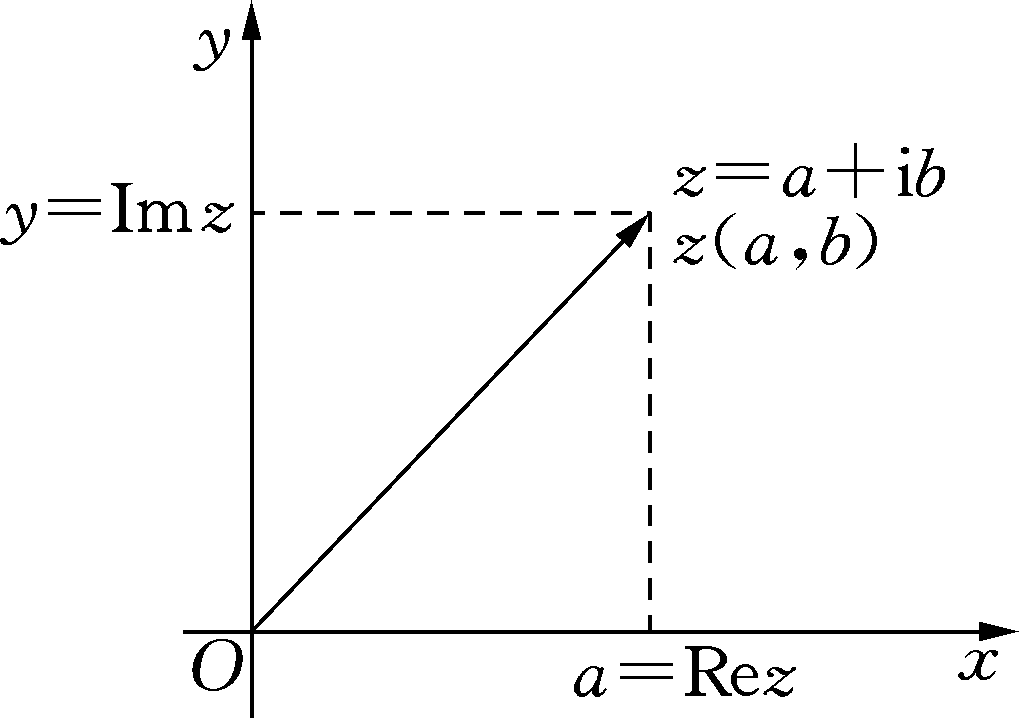
\includegraphics[keepaspectratio,alt={图1.1 复平面与共轭复数}]{figures/01-复数和复平面/fig-p03-c08450d4.png}}
\caption{图1.1 复平面与共轭复数}
\end{figure}

\subsection{1.1.3 复数的模}\label{ux590dux6570ux7684ux6a21}

在复平面上，复数 \(z=a+ib\) 还可用由原点 \(O\) 引向点 \(z\) 的向量
\(\overrightarrow{Oz}\) 表示。该向量的长度称为复数 \(z\)
的\textbf{模}，记作 \(|z|\)（或 \(r\)）：

\[
|z| = r = \sqrt{a^2+b^2} \ge 0 .
\]

模与实部、虚部满足

\[
|\operatorname{Re} z| \le |z| \le |\operatorname{Re} z| + |\operatorname{Im} z|,
\qquad
|\operatorname{Im} z| \le |z| \le |\operatorname{Re} z| + |\operatorname{Im} z| .
\]

\subsection{1.1.4
复数的四则运算}\label{ux590dux6570ux7684ux56dbux5219ux8fd0ux7b97}

设 \(z_1=a+ib\)，\(z_2=c+id\)。

\textbf{加法}

\[
z_1+z_2 = (a+c)+i(b+d).
\]

\textbf{减法}

\[
z_1-z_2 = (a-c)+i(b-d).
\]

\textbf{乘法}

\[
z_1 z_2 = (a+ib)(c+id) = (ac-bd)+i(ad+bc),
\qquad
z^2 = z\cdot z .
\]

\textbf{除法}

\[
\frac{z_1}{z_2}
= \frac{a+ib}{c+id}
= \frac{(a+ib)(c-id)}{(c+id)(c-id)}
= \frac{ac+bd}{c^2+d^2} + i\,\frac{bc-ad}{c^2+d^2},\qquad z_2\neq 0 .
\]

\begin{figure}
\centering
\pandocbounded{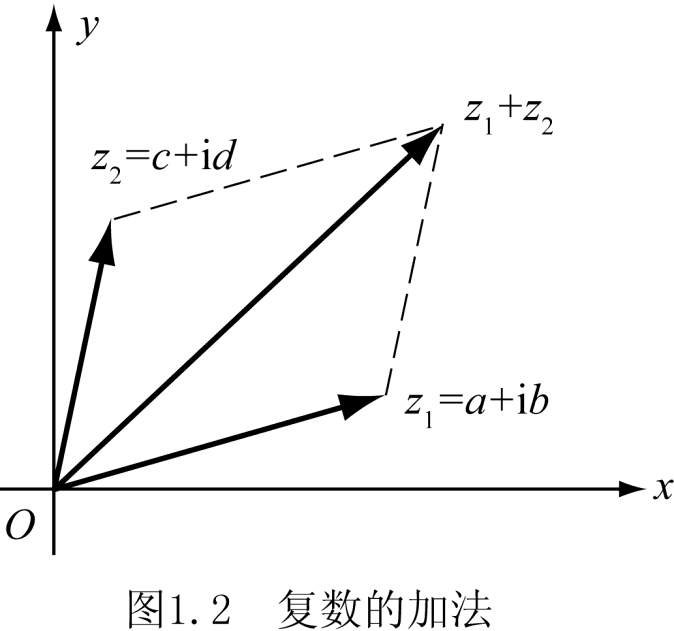
\includegraphics[keepaspectratio,alt={图1.2 复数的加法}]{figures/01-复数和复平面/fig-p04-37af5db3.png}}
\caption{图1.2 复数的加法}
\end{figure}

\subsection{1.1.5
模与共轭复数的性质}\label{ux6a21ux4e0eux5171ux8f6dux590dux6570ux7684ux6027ux8d28}

设 \(z,w \in \mathbb{C}\)，\(w\neq 0\)，则

\[
\begin{aligned}
&(1)\ \operatorname{Re} z = \frac{z+\bar z}{2},\qquad
\operatorname{Im} z = \frac{z-\bar z}{2i};\\[2pt]
&(2)\ \overline{z\pm w} = \bar z \pm \bar w,\qquad
\overline{zw} = \bar z\,\bar w,\qquad
\overline{\left(\frac{z}{w}\right)} = \frac{\bar z}{\bar w};\\[2pt]
&(3)\ z\bar z = |z|^2,\qquad
(4)\ \overline{\bar z} = z,\qquad
(5)\ z+\bar z = 2\operatorname{Re} z,\quad z-\bar z = 2i\operatorname{Im} z .
\end{aligned}
\]

\subsection{1.1.6
复数的三角表示与指数形式}\label{ux590dux6570ux7684ux4e09ux89d2ux8868ux793aux4e0eux6307ux6570ux5f62ux5f0f}

设复平面 \(\mathbb{C}\) 上不为零的点 \(z=x+iy\)，取极坐标

\[
x = r\cos\theta,\qquad y = r\sin\theta,\qquad r=|z| .
\]

\(\theta\) 是正实轴与从原点 \(O\) 到 \(z\) 的射线的夹角，称为复数 \(z\)
的\textbf{辐角}，记作 \(\theta=\operatorname{Arg}z\)。满足

\[
-\pi < \theta \le \pi
\]

的辐角称为 \(\operatorname{Arg}z\) 的\textbf{主值}，记作
\(\theta=\arg z\)，于是

\[
\operatorname{Arg} z = \arg z + 2k\pi,\quad k=0,\pm1,\pm2,\ldots .
\]

复数 \(z\) 有\textbf{三角表示}与\textbf{指数表示}：

\[
z = r(\cos\theta+i\sin\theta)
\qquad\text{与}\qquad
z = re^{i\theta}.
\]

\begin{figure}
\centering
\pandocbounded{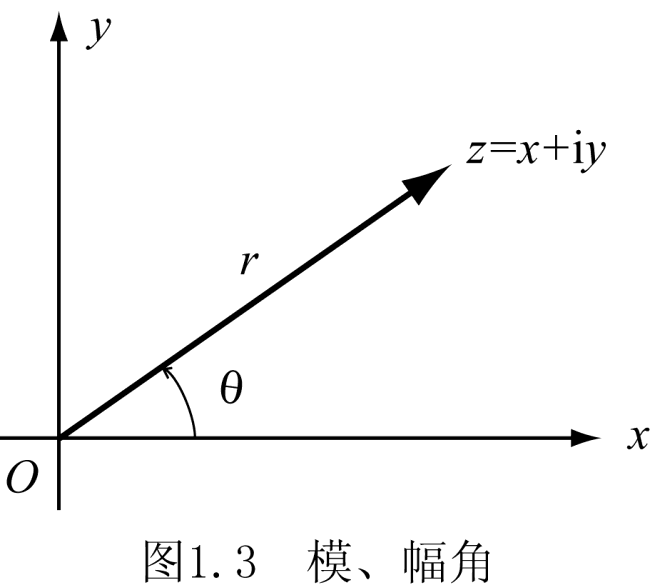
\includegraphics[keepaspectratio,alt={图1.3 极坐标下的复数}]{figures/01-复数和复平面/fig-p06-19f16d72.png}}
\caption{图1.3 极坐标下的复数}
\end{figure}

\textbf{例 1.1} 求 \(\operatorname{Arg}(-3-4i)\)。

\textbf{解} \((-3,-4)\) 位于第三象限，

\[
\arg(-3-4i) = \arctan\frac{4}{3}-\pi,
\]

所以

\[
\operatorname{Arg}(-3-4i)
= \arg(-3-4i)+2k\pi
= \arctan\frac{4}{3} + (2k-1)\pi,
\qquad k=0,\pm1,\pm2,\ldots .
\]

\textbf{例 1.2} 计算 \(z=e^{i\pi}\)。

\textbf{解}

\[
e^{i\pi} = \cos\pi + i\sin\pi = -1 .
\]

\textbf{例 1.3} 把 \(\sqrt3+i\) 表示成三角形式和指数形式。

\textbf{解}
\(r=|\sqrt3+i|=\sqrt{3+1}=2\)，\(\cos\theta=\sqrt3/2\)，点在第一象限，故
\(\theta=\arg(\sqrt3+i)=\pi/6\)，从而

\[
\sqrt3+i = 2\left(\cos\frac{\pi}{6}+i\sin\frac{\pi}{6}\right) = 2e^{i\pi/6}.
\]

\subsection{1.1.7
复数乘除法的几何意义}\label{ux590dux6570ux4e58ux9664ux6cd5ux7684ux51e0ux4f55ux610fux4e49}

设

\[
z_1 = r_1(\cos\theta_1+i\sin\theta_1),\qquad
z_2 = r_2(\cos\theta_2+i\sin\theta_2),
\]

利用三角恒等式可得

\[
\begin{aligned}
z_1z_2
&= r_1r_2\bigl[(\cos\theta_1\cos\theta_2-\sin\theta_1\sin\theta_2)
+i(\sin\theta_1\cos\theta_2+\cos\theta_1\sin\theta_2)\bigr]\\[2pt]
&= r_1r_2\bigl[\cos(\theta_1+\theta_2)+i\sin(\theta_1+\theta_2)\bigr],
\end{aligned}
\]

即

\[
|z_1z_2| = r_1r_2 = |z_1|\,|z_2|,
\qquad
\operatorname{Arg}(z_1z_2) = \operatorname{Arg}z_1+\operatorname{Arg}z_2 .
\]

\textbf{两个复数相乘：积的模等于各复数模的积，积的辐角等于两复数辐角的和。}

类似地，

\[
\left|\frac{z_1}{z_2}\right| = \frac{|z_1|}{|z_2|},
\qquad
\operatorname{Arg}\frac{z_1}{z_2} = \operatorname{Arg}z_1 - \operatorname{Arg}z_2 .
\]

\begin{figure}
\centering
\pandocbounded{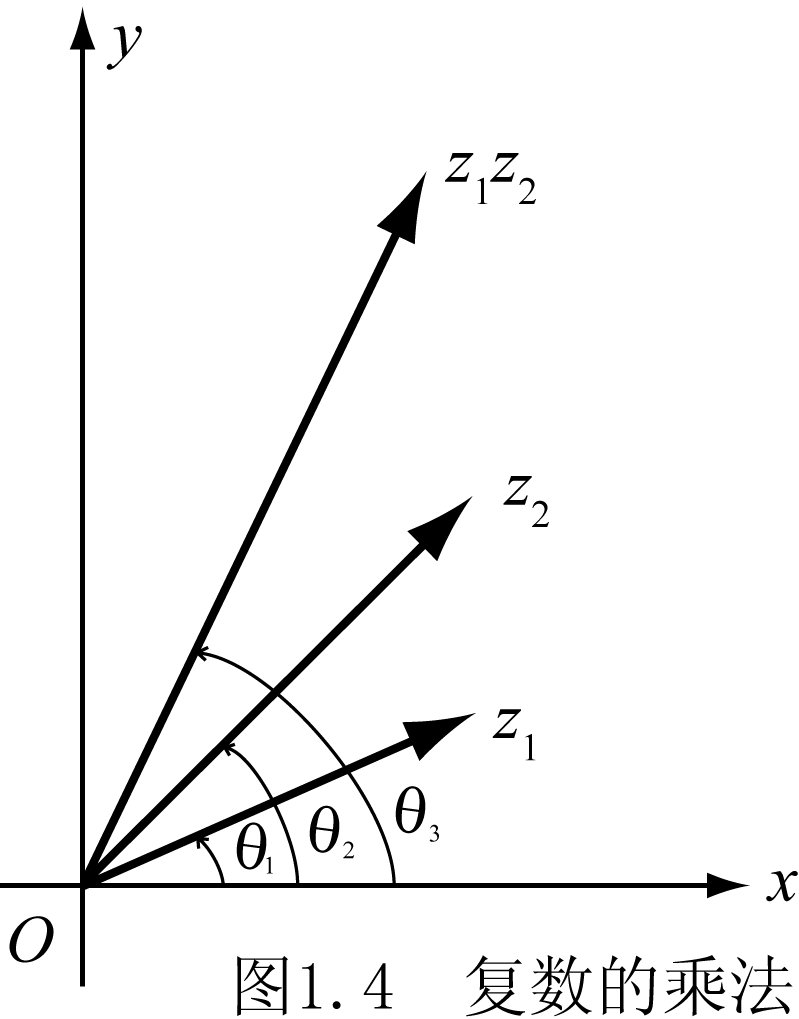
\includegraphics[keepaspectratio,alt={图1.4 复数的乘法}]{figures/01-复数和复平面/fig-p09-23c42b74.png}}
\caption{图1.4 复数的乘法}
\end{figure}

\subsection{1.1.8
复数的乘方与开方}\label{ux590dux6570ux7684ux4e58ux65b9ux4e0eux5f00ux65b9}

\textbf{乘方} 设 \(z=re^{i\theta}\)，则

\[
z^n = \left(re^{i\theta}\right)^n = r^n e^{in\theta}
= r^n(\cos n\theta+i\sin n\theta),
\qquad
|z^n| = |z|^n .
\]

当 \(r=1\) 时，得到 \textbf{棣莫弗（de Moivre）公式}：

\[
(\cos\theta+i\sin\theta)^n = \cos n\theta + i\sin n\theta .
\]

\textbf{开方} 设 \(z=re^{i\theta}\) 是已知复数，\(n\) 为正整数，满足方程

\[
\omega^n = z
\]

的全体复数 \(\omega\) 称为 \(z\) 的 \textbf{\(n\) 次方根}，记作
\(\omega=\sqrt[n]{z}\)。

设 \(\omega=\rho e^{i\varphi}\)，由
\(\rho^n e^{in\varphi}=re^{i\theta}\) 得

\[
\rho = \sqrt[n]{r},\qquad
\varphi = \frac{\theta+2k\pi}{n},\quad k=0,1,\ldots,n-1,
\]

所以

\[
\sqrt[n]{z} = \omega_k
= \sqrt[n]{r}\,e^{i\frac{\theta+2k\pi}{n}},
\qquad k=0,1,2,\ldots,n-1 .
\]

复数的 \(n\) 次方根共有 \(n\) 个：它们的模都等于该复数模的 \(n\)
次算术根，辐角分别等于该复数辐角与 \(0,1,\ldots,n-1\) 倍 \(2\pi\) 之和的
\(n\) 分之一。

\begin{figure}
\centering
\pandocbounded{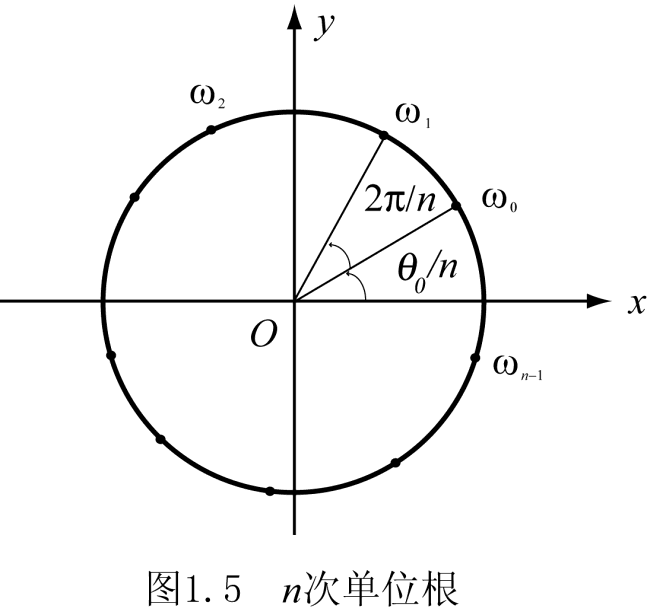
\includegraphics[keepaspectratio,alt={图1.5 n 次方根}]{figures/01-复数和复平面/fig-p12-42098742.png}}
\caption{图1.5 n 次方根}
\end{figure}

\textbf{例 1.4} 求 \(1-i\) 的立方根。

\textbf{解} 先写指数形式：

\[
1-i = \sqrt2\,e^{i7\pi/4},
\]

则

\[
\sqrt[3]{1-i}
= 2^{1/6}e^{i\frac{7\pi/4+2k\pi}{3}}
= 2^{1/6}e^{i\left(\frac{7\pi}{12}+\frac{2k\pi}{3}\right)},
\qquad k=0,1,2 .
\]

即三个立方根为

\[
2^{1/6}e^{i7\pi/12},\qquad
2^{1/6}e^{i5\pi/4},\qquad
2^{1/6}e^{i23\pi/12}.
\]

\textbf{例 1.5} 计算 \(n\) 次单位根。

\textbf{解} \(1=e^{i0}\)，故 \(n\) 次单位根为

\[
1,\quad e^{i\frac{2\pi}{n}},\quad e^{i\frac{4\pi}{n}},\quad \ldots,\quad
e^{i\frac{2(n-1)\pi}{n}} .
\]

立方单位根为

\[
1,\qquad \frac{-1+i\sqrt3}{2},\qquad \frac{-1-i\sqrt3}{2}.
\]

\subsection{常见错误与注意点}\label{ux5e38ux89c1ux9519ux8befux4e0eux6ce8ux610fux70b9}

\begin{enumerate}
\def\labelenumi{\arabic{enumi}.}
\tightlist
\item
  \textbf{辐角是多值的}：\(\operatorname{Arg}z\) 与 \(\arg z\)
  不可混用；写 \(\operatorname{Arg}z\) 时务必补 \(2k\pi\)。
\item
  \textbf{开方记号的约定}：\(\sqrt[n]{z}\) 表示 \(n\)
  个值；实数范围内``根号''的单值约定在复数范围内不再成立。
\item
  \textbf{分母不为零}：作除法 \(z_1/z_2\) 时，必须先说明 \(z_2\neq 0\)。
\item
  \textbf{点 \((a,b)\) vs 向量
  \(\overrightarrow{Oz}\)}：复平面中同一个复数既可看作点，也可看作向量，两者都常用。
\end{enumerate}

\subsection{本节小结}\label{ux672cux8282ux5c0fux7ed3}

\begin{itemize}
\tightlist
\item
  复数 \(z=a+ib\)：实部/虚部、共轭、模、辐角；
\item
  运算：加减乘除、乘方、开方；
\item
  几何意义：乘 = 模相乘 + 辐角相加；除 = 模相除 + 辐角相减；
\item
  工具：三角形式 \(z=r(\cos\theta+i\sin\theta)\) 与指数形式
  \(z=re^{i\theta}\)。
\end{itemize}

\section{1.2 复平面点集}\label{ux590dux5e73ux9762ux70b9ux96c6}

\begin{quote}
本节目标：掌握复平面中的邻域、内点、开集、边界、区域、曲线、连通性等基础概念，会用集合语言描述平面图形。
重点：区域的定义、简单闭曲线、单连通与多连通区域。
难点：直线与半平面的复数表示。
\end{quote}

\subsection{1.2.1
平面点集的几个概念}\label{ux5e73ux9762ux70b9ux96c6ux7684ux51e0ux4e2aux6982ux5ff5}

\textbf{（1）邻域} 集合

\[
D(z_0,\delta) = \{\, z : |z-z_0|<\delta\,\},\qquad \delta>0
\]

称为 \(z_0\) 的 \(\delta\) \textbf{邻域}；而去心邻域为

\[
D(z_0,\delta)\setminus\{z_0\} = \{\, z : 0<|z-z_0|<\delta\,\}.
\]

\textbf{（2）内点、开集} 若点集 \(E\) 的点 \(z_0\) 存在一个邻域
\(D(z_0,\delta)\subset E\)，则称 \(z_0\) 为 \(E\)
的一个\textbf{内点}；若 \(E\) 中的点全为内点，则称 \(E\)
为\textbf{开集}。

\textbf{（3）边界点、边界} 若点 \(z_0\) 的任意邻域内既有属于 \(E\)
的点、又有不属于 \(E\) 的点，则称 \(z_0\) 为 \(E\)
的\textbf{边界点}；\(E\) 的所有边界点组成的集合称为 \(E\)
的\textbf{边界}，记作 \(\partial E\)。

\textbf{（4）区域} 若 \(E\) 内任何两点都可用包含在 \(E\)
内的一条折线连接起来，则称 \(E\)
为\textbf{连通集}。\textbf{连通的开集称为区域}。区域 \(D\) 与其边界
\(\partial D\) 的并集称为\textbf{闭区域}，记为 \(\bar D\)。

\textbf{（5）有界区域} 若存在正数 \(M\)，使得对一切 \(z\in E\) 有
\(|z|\le M\)，则称 \(E\)
为\textbf{有界集}；有界的区域称为\textbf{有界区域}。

\subsection{1.2.2
简单曲线与光滑曲线}\label{ux7b80ux5355ux66f2ux7ebfux4e0eux5149ux6ed1ux66f2ux7ebf}

设 \(x(t)\) 与 \(y(t)\) 是实变量 \(t\) 的两个实函数，在闭区间
\([\alpha,\beta]\) 上连续，则方程组

\[
\begin{cases}
x = x(t),\\
y = y(t),
\end{cases}
\qquad t\in[\alpha,\beta]
\]

或复值函数

\[
z(t) = x(t)+iy(t)
\]

确定的集合称为复平面上的一条\textbf{曲线}，上述方程称为曲线的\textbf{参数方程}。

点 \(A=z(\alpha)\) 与 \(B=z(\beta)\) 分别称为曲线的起点和终点。若当
\(t_1\neq t_2\)（\(t_1,t_2\in[\alpha,\beta]\)）时，\(z(t_1)\neq z(t_2)\)，则称曲线为\textbf{简单曲线}（\textbf{约当
Jordan 曲线}）。若
\(z(\alpha)=z(\beta)\)，则简单曲线称为\textbf{简单闭曲线}。

\textbf{定理 1.1（约当定理）}
一条简单闭曲线把平面分成两个不相交的区域，以该曲线为公共边界。其中一个是有界的，称为曲线的\textbf{内部}；另一个是无界的，称为曲线的\textbf{外部}。

若曲线 \(\Gamma\) 在 \([\alpha,\beta]\) 上 \(x'(t)\)、\(y'(t)\)
存在、连续且不同时为零，则称 \(\Gamma\)
为\textbf{光滑曲线}；由有限条光滑曲线连接而成的连续曲线称为\textbf{分段光滑曲线}。

\subsection{1.2.3
单连通区域与多连通区域}\label{ux5355ux8fdeux901aux533aux57dfux4e0eux591aux8fdeux901aux533aux57df}

\textbf{（7）单连通区域} 设 \(D\) 为复平面上的区域，若 \(D\)
内任意简单闭曲线的内部仍属于 \(D\)，则称 \(D\)
为\textbf{单连通区域}；否则称为\textbf{多连通区域}。

\begin{quote}
直观理解：单连通区域``没有洞''；多连通区域``有洞''（如圆环域）。
\end{quote}

\subsection{1.2.4
直线与半平面}\label{ux76f4ux7ebfux4e0eux534aux5e73ux9762}

设 \(L\) 表示 \(\mathbb{C}\) 中的直线，\(a\) 是 \(L\) 上的任一点，\(b\)
为它的方向向量，则

\[
L = \{\, z : z = a+tb,\ t\in(-\infty,+\infty)\,\}.
\]

对 \(L\) 上的 \(z\)，有

\[
\operatorname{Im}\frac{z-a}{b} = 0 .
\]

由不等式可以定义两个半平面：

\[
L:\ \operatorname{Im}\frac{z-a}{b} = 0,
\qquad
H_0:\ \operatorname{Im}\frac{z-a}{b} > 0,
\qquad
K_0:\ \operatorname{Im}\frac{z-a}{b} < 0 .
\]

为方便，假定 \(|b|=1\) 且 \(a=0\)。令
\(b=e^{i\beta}\)，\(z=re^{i\theta}\)，则

\[
\frac{z}{b} = re^{i(\theta-\beta)},
\]

于是 \(z\in H_0\) 当且仅当 \(\operatorname{Im}\frac{z}{b}>0\)，即

\[
\sin(\theta-\beta)>0
\quad\Longleftrightarrow\quad
\beta<\theta<\beta+\pi .
\]

若``按 \(b\) 的方向沿 \(L\) 前进''，则 \(H_0\) 是位于 \(L\)
\textbf{左边}的半平面；由平移可得

\[
H_a = \{\, w : w=a+h,\ h\in H_0\,\} = \left\{\,z : \operatorname{Im}\frac{z-a}{b}>0\,\right\}
\]

是位于 \(L\) 左边的半平面，而

\[
K_a = \left\{\,z : \operatorname{Im}\frac{z-a}{b}<0\,\right\}
\]

是位于 \(L\) 右边的半平面。

\subsection{常见错误与注意点}\label{ux5e38ux89c1ux9519ux8befux4e0eux6ce8ux610fux70b9-1}

\begin{enumerate}
\def\labelenumi{\arabic{enumi}.}
\tightlist
\item
  ``连通的开集是区域''是标准定义；不要漏掉``开集''这一条件。
\item
  边界点不要求属于集合本身：闭区域 \(\bar D=D\cup\partial D\) 包含边界。
\item
  简单曲线可以自交？不可以；简单曲线要求不同的参数对应不同的点。
\item
  半平面的判别式 \(\operatorname{Im}\frac{z-a}{b}\) 的正负与方向向量
  \(b\) 的选择有关。
\end{enumerate}

\subsection{本节小结}\label{ux672cux8282ux5c0fux7ed3-1}

\begin{itemize}
\tightlist
\item
  邻域、内点、开集、边界、区域、闭区域、有界区域；
\item
  曲线、简单曲线、简单闭曲线、光滑曲线、分段光滑曲线；
\item
  约当定理：简单闭曲线划分内部与外部；
\item
  单连通/多连通区域；
\item
  直线与半平面：\(\operatorname{Im}\frac{z-a}{b}\gtrless 0\)。
\end{itemize}

\section{1.3
扩充复平面及其球面表示}\label{ux6269ux5145ux590dux5e73ux9762ux53caux5176ux7403ux9762ux8868ux793a}

\begin{quote}
本节目标：理解无穷远点 \(\infty\)
的引入方式、扩充复平面的运算约定以及球面（黎曼球面）表示。
重点：扩充复平面 \(\mathbb{C}_\infty\)；无穷远点的球面模型。
难点：为什么无穷远点只有一个；哪些运算不规定意义。
\end{quote}

\subsection{1.3.1
扩充复平面的运算约定}\label{ux6269ux5145ux590dux5e73ux9762ux7684ux8fd0ux7b97ux7ea6ux5b9a}

设 \(a\) 是异于 \(\infty\) 的一个复数，规定：

\[
\begin{aligned}
&(1)\ a\neq\infty \ \Rightarrow\ a\pm\infty = \infty\pm a = \infty;\\[2pt]
&(2)\ a\neq 0 \ \Rightarrow\ a\cdot\infty = \infty\cdot a = \infty;\\[2pt]
&(3)\ a\neq\infty \ \Rightarrow\ \frac{a}{\infty}=0,\qquad
a\neq 0 \ \Rightarrow\ \frac{\infty}{a}=\infty .
\end{aligned}
\]

\(\infty\)
的实部、虚部、辐角都无意义。为了避免与算术定律矛盾，对下列式子\textbf{不规定意义}：

\[
\infty\pm\infty,\qquad \infty\cdot 0,\qquad 0\cdot\infty,\qquad \frac{0}{\infty},\qquad \frac{\infty}{\infty},\qquad \frac{\infty}{0}.
\]

\subsection{1.3.2 扩充复平面}\label{ux6269ux5145ux590dux5e73ux9762}

设想平面上有一个``理想点''与 \(\infty\)
对应，称为\textbf{无穷远点}。复平面加上
\(\infty\)，称为\textbf{扩充复平面}：

\[
\mathbb{C}_\infty = \mathbb{C}\cup\{\infty\}.
\]

为使运算法则合理，规定\textbf{扩充复平面上只有一个无穷远点}。

\subsection{1.3.3
球面表示（黎曼球面）}\label{ux7403ux9762ux8868ux793aux9eceux66fcux7403ux9762}

记 \(\mathbb{R}^3\) 中的单位球面为

\[
S = \{(x_1,x_2,x_3): x_1^2+x_2^2+x_3^2=1\},
\qquad N=(0,0,1)\ \text{为北极点}.
\]

把复平面 \(\mathbb{C}\) 等同于 \(\mathbb{R}^3\) 中的点集

\[
\{(x_1,x_2,0): x_1,x_2\in\mathbb{R}\}.
\]

对复平面内任意一点 \(z\)，用直线将 \(z\) 与北极点 \(N\)
相连，该直线与球面 \(S\) 恰交于一点
\(Z\neq N\)。这个对应给出复平面到``去北极点的球面''的一一映射，称为\textbf{球面投影（stereographic
projection）}。

\begin{itemize}
\tightlist
\item
  若 \(|z|>1\)，则 \(Z\) 位于北半球面上；
\item
  若 \(|z|<1\)，则 \(Z\) 位于南半球面上；
\item
  若 \(|z|=1\)，则 \(Z=z\)；
\item
  当 \(|z|\to\infty\) 时，\(Z\to N\)。
\end{itemize}

于是\textbf{扩充复平面 \(\mathbb{C}_\infty\) 与整个球面 \(S\)（含北极点
\(N\)）一一对应}；北极点 \(N\) 正好对应无穷远点
\(\infty\)。这一模型称为\textbf{黎曼球面}。

\subsection{常见错误与注意点}\label{ux5e38ux89c1ux9519ux8befux4e0eux6ce8ux610fux70b9-2}

\begin{enumerate}
\def\labelenumi{\arabic{enumi}.}
\tightlist
\item
  \(\infty\)
  只有一个：复平面不是``四面八方无穷远''，而是``一个无穷远点''。
\item
  不能把 \(\infty\)
  当成普通复数参与四则运算；\(\infty\pm\infty\)、\(\infty\cdot 0\)
  等均不定义。
\item
  球面投影中，\(|z|\) 越大越接近北极，但不等于``正无穷''有多个方向。
\end{enumerate}

\subsection{本节小结}\label{ux672cux8282ux5c0fux7ed3-2}

\begin{itemize}
\tightlist
\item
  \(\mathbb{C}_\infty=\mathbb{C}\cup\{\infty\}\)；
\item
  无穷远点的运算约定与禁用式；
\item
  黎曼球面：复平面去掉一点（北极点）与球面同胚，\(z\to\infty\)
  对应北极点。
\end{itemize}

\section{第1章
本章小结与教学建议}\label{ux7b2c1ux7ae0-ux672cux7ae0ux5c0fux7ed3ux4e0eux6559ux5b66ux5efaux8bae}

\subsection{知识框架}\label{ux77e5ux8bc6ux6846ux67b6}

\begin{enumerate}
\def\labelenumi{\arabic{enumi}.}
\tightlist
\item
  复数：概念、相等、共轭、模、辐角（主值）、三角形式、指数形式；
\item
  运算：加减乘除、乘方（棣莫弗公式）、开方（n 个 n 次方根）；
\item
  几何：复平面上的点/向量表示，乘除法的模与辐角规律；
\item
  点集语言：邻域、内点、开集、边界、区域、闭区域、有界、曲线、单连通；
\item
  扩充复平面：\(\mathbb{C}_\infty = \mathbb{C}\cup\{\infty\}\)，黎曼球面模型。
\end{enumerate}

\subsection{教学建议}\label{ux6559ux5b66ux5efaux8bae}

\begin{itemize}
\tightlist
\item
  第1节宜慢讲：学生的困惑主要在``辐角的多值性''和``\(z\)
  既是点又是向量''；
\item
  乘除法的几何意义建议配合图形（复平面上的向量加法和乘法图）讲解；
\item
  开方一节可与后续``解析函数的多值性''呼应；
\item
  点集概念是第2、3章的基础，建议把``区域''与``单连通''作为重点，多举例（圆盘、圆环、去心圆盘、半平面）；
\item
  球面表示可作为选讲内容，帮助理解 \(\infty\)。
\end{itemize}

\subsection{常见考点提示}\label{ux5e38ux89c1ux8003ux70b9ux63d0ux793a}

\begin{itemize}
\tightlist
\item
  已知 \(z\)，求
  \(\operatorname{Re}z,\operatorname{Im}z,|z|,\bar z,\operatorname{Arg}z\)；
\item
  将复数化为三角/指数形式；
\item
  求 \(n\) 次方根、\(n\) 次单位根；
\item
  判断平面图形（圆、圆环、角域、半平面等）并写出集合表达式；
\item
  判断区域是否单连通。
\end{itemize}

\newpage

\chaptercover{2}{解析函数}
%% 由 build/emit_tex.py 生成（生成物，勿手改）；定制请放 user_style.tex / user_meta.yaml
\chapter{第 2 章 ·
解析函数}\label{ux7b2c-2-ux7ae0-ux89e3ux6790ux51fdux6570}

\section{§2.1
复变函数的概念、极限与连续性}\label{ux590dux53d8ux51fdux6570ux7684ux6982ux5ff5ux6781ux9650ux4e0eux8fdeux7eedux6027}

\begin{quote}
\textbf{本节目标}：掌握复变函数的概念、几何意义（映射）、反函数；理解复变函数极限的
\(\varepsilon\)-\(\delta\)
定义及其与二元实函数极限的联系；掌握复变函数连续的概念与判定。
\textbf{本节重点}：复变函数作为两个复平面上点集间的映射；极限与连续的概念；用实部/虚部函数研究极限与连续性。
\textbf{本节难点}：极限存在的充要条件（与二元实函数极限的等价性）；\(\arg z\)
的连续性（负实轴上的间断）。
\end{quote}

\subsection{2.1.1
复变函数的概念}\label{ux590dux53d8ux51fdux6570ux7684ux6982ux5ff5}

\textbf{定义 2.1} 设 \(E\) 为一复数集。若对 \(E\) 中每一个复数
\(z=x+iy\)，按照某种法则 \(f\) 有确定的一个或几个复数 \(w=u+iv\)
与之对应，那么称复变数 \(w\) 是复变数 \(z\)
的函数（简称\textbf{复变函数}），记作

\[
w=f(z).
\]

通常也称 \(w=f(z)\) 为定义在 \(E\) 上的复变函数，其中 \(E\)
称为\textbf{定义域}，\(E\) 中所有 \(z\) 对应的一切 \(w\)
值构成的集合称为 \(f(z)\) 的\textbf{值域}，记作 \(f(E)\) 或 \(G\)。

\begin{itemize}
\tightlist
\item
  若 \(z\) 的一个值对应着 \(w\) 的一个值，则称复变函数 \(f(z)\)
  是\textbf{单值}的；
\item
  若 \(z\) 的一个值对应着 \(w\) 的两个或两个以上的值，则称复变函数
  \(f(z)\) 是\textbf{多值}的。
\end{itemize}

\subsubsection{实部与虚部}\label{ux5b9eux90e8ux4e0eux865aux90e8}

复数 \(z=x+iy\) 与 \(w=u+iv\) 分别对应实数对 \((x,y)\) 和
\((u,v)\)。对于函数 \(w=f(z)\)，\(u\)、\(v\) 为 \(x\)、\(y\)
的二元实函数 \(u(x,y)\) 和 \(v(x,y)\)，所以 \(w=f(z)\) 又常写成

\[
w=f(z)=u(x,y)+iv(x,y).
\]

\textbf{例（\(w=z^2+1\)）} 令 \(z=x+iy\)，\(w=u+iv\)，那么

\[
w=u+iv=(x+iy)^2+1=x^2-y^2+1+2xyi,
\]

\(w=z^2+1\) 对应于两个实函数

\[
u=x^2-y^2+1,\qquad v=2xy.
\]

\subsubsection{复变函数的映射（几何）意义}\label{ux590dux53d8ux51fdux6570ux7684ux6620ux5c04ux51e0ux4f55ux610fux4e49}

对于复变函数 \(w=f(z)\) 即
\(u+iv=f(x+iy)\)，可以理解为两个复平面上的点集之间的映射。具体地说，复变函数
\(w=f(z)\) 给出了 \(z\) 平面上的点集 \(E\) 到 \(w\) 平面上的点集
\(f(E)\)（或 \(G\)）之间的一个对应关系：

\[
\forall z\in E \rightarrow w=f(z)\in G .
\]

其中 \(w\) 称为 \(z\) 的\textbf{像}，\(z\) 称为 \(w\) 的\textbf{原像}。

\begin{figure}
\centering
\pandocbounded{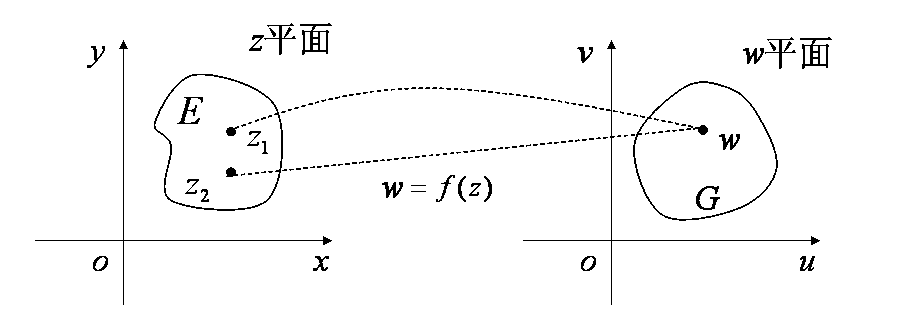
\includegraphics[keepaspectratio,alt={图2.1 复变函数的映射}]{figures/02-解析函数/fig-p03-a37f4956.png}}
\caption{图2.1 复变函数的映射}
\end{figure}

\subsubsection{反函数}\label{ux53cdux51fdux6570}

设函数 \(w=f(z)\) 定义在 \(E\) 上，值域为 \(G\)。若对于 \(G\) 中的任一点
\(w\)，在 \(E\) 中存在一个或几个点 \(z\) 与之对应，则在 \(G\)
上确定了一个单值或多值函数，记作 \(z=f^{-1}(w)\)，称为函数 \(w=f(z)\)
的\textbf{反函数}。

\textbf{例 2.1} 函数 \(\displaystyle w=\frac{1}{z}\) 将 \(z\)
平面上的直线 \(x=1\) 变成 \(w\) 平面上的何种曲线？

\textbf{解} 令 \(z=x+iy\)，\(w=u+iv\)，则

\[
w=u+iv=\frac{1}{z}=\frac{1}{x+iy}=\frac{x-iy}{x^2+y^2},
\]

故

\[
u=\frac{x}{x^2+y^2},\qquad v=-\frac{y}{x^2+y^2}.
\]

\(z\) 平面上的直线 \(x=1\) 对应于 \(w\) 平面上的曲线

\[
u=\frac{1}{1+y^2},\qquad v=-\frac{y}{1+y^2}.
\]

于是

\[
u^2+v^2
=\frac{1}{(1+y^2)^2}+\frac{y^2}{(1+y^2)^2}
=\frac{1}{1+y^2}=u,
\]

即

\[
\left(u-\frac{1}{2}\right)^2+v^2=\frac{1}{4}.
\]

所以直线 \(x=1\) 被映射为 \(w\) 平面上以 \(\left(\dfrac{1}{2},0\right)\)
为圆心、\(\dfrac{1}{2}\) 为半径的圆。

\begin{figure}
\centering
\pandocbounded{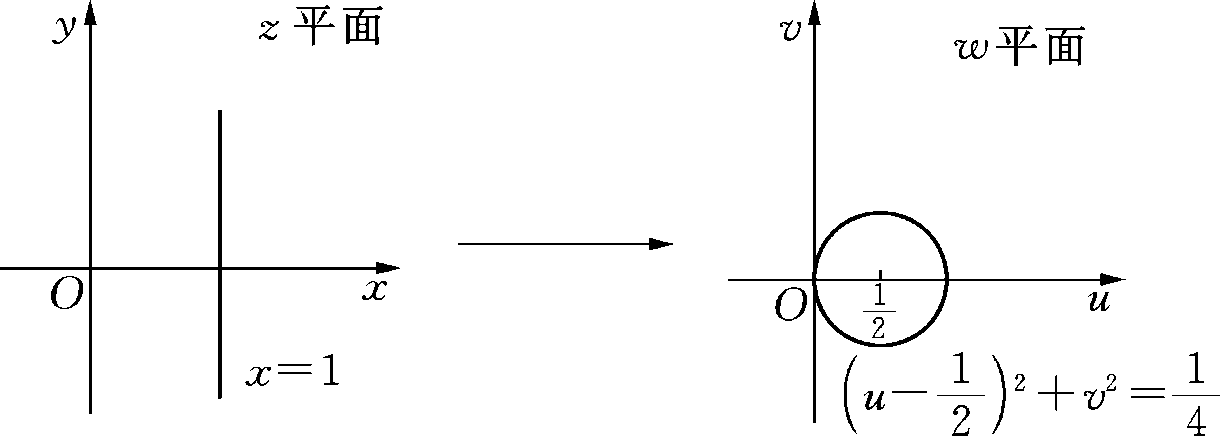
\includegraphics[keepaspectratio,alt={图2.2 例2.1 直线 x=1 的像}]{figures/02-解析函数/fig-p04-7f4c02e9.png}}
\caption{图2.2 例2.1 直线 x=1 的像}
\end{figure}

\subsection{2.1.2
复变函数的极限}\label{ux590dux53d8ux51fdux6570ux7684ux6781ux9650}

\textbf{定义 2.2} 设函数 \(w=f(z)\) 定义在 \(z_0\) 的去心邻域
\(0<|z-z_0|<r\) 内。若存在常数 \(A\)，对于任意给定的
\(\varepsilon>0\)，都存在一正数 \(\delta\)（\(0<\delta\le r\)），使得当
\(0<|z-z_0|<\delta\) 时，有

\[
|f(z)-A|<\varepsilon,
\]

则称函数 \(f(z)\) 当 \(z\to z_0\) 时的极限存在，常数 \(A\)
为其极限值，记作

\[
\lim_{z\to z_0}f(z)=A
\qquad\text{或}\qquad
f(z)\to A\ (z\to z_0).
\]

\textbf{几何意义} 当变点 \(z\) 进入 \(z_0\)
的充分小的去心邻域时，它的像点 \(f(z)\) 就落入 \(A\)
的一个预先给定的邻域内。

\begin{quote}
定义中 \(z\to z_0\) 的方式是任意的：\(z\) 在 \(z_0\)
的去心邻域内沿任何曲线以任何方式趋于 \(z_0\) 时，\(f(z)\)
都要趋向于同一个常数 \(A\)。
\end{quote}

\begin{figure}
\centering
\pandocbounded{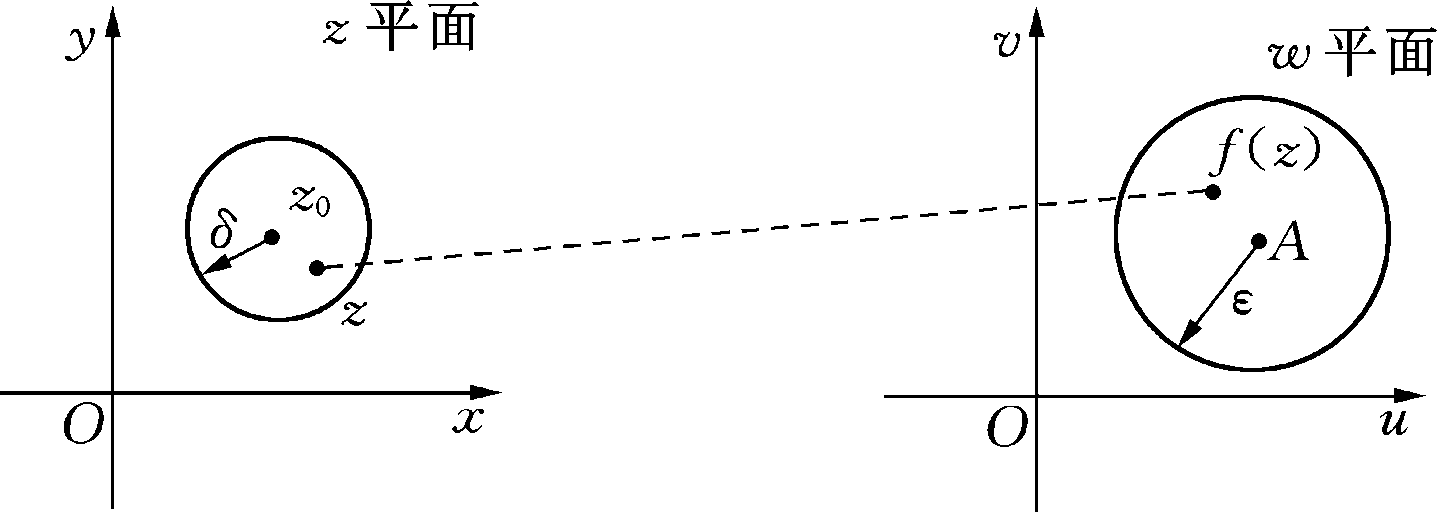
\includegraphics[keepaspectratio,alt={图2.3 极限的几何意义}]{figures/02-解析函数/fig-p06-bc429569.png}}
\caption{图2.3 极限的几何意义}
\end{figure}

\textbf{定理 2.1} 设
\(f(z)=u(x,y)+iv(x,y)\)，\(z_0=x_0+iy_0\)，\(A=a+ib\)，则

\[
\lim_{z\to z_0}f(z)=A
\iff
\lim_{(x,y)\to(x_0,y_0)}u(x,y)=a,\quad
\lim_{(x,y)\to(x_0,y_0)}v(x,y)=b .
\]

\textbf{证明要点}

\begin{itemize}
\tightlist
\item
  \textbf{必要性}：设 \(\lim_{z\to z_0}f(z)=A\)，即对任意
  \(\varepsilon>0\)，存在 \(\delta>0\)，当
\end{itemize}

\[
0<|z-z_0|=\sqrt{(x-x_0)^2+(y-y_0)^2}<\delta
\]

时，有

\[
|f(z)-A|=\sqrt{(u-a)^2+(v-b)^2}<\varepsilon .
\]

由于
\(|u-a|\le\sqrt{(u-a)^2+(v-b)^2}\)，\(|v-b|\le\sqrt{(u-a)^2+(v-b)^2}\)，故
\(|u-a|<\varepsilon\)、\(|v-b|<\varepsilon\)，从而两个实函数极限成立。

\begin{itemize}
\tightlist
\item
  \textbf{充分性}：设两个实函数极限成立，则当
  \(\sqrt{(x-x_0)^2+(y-y_0)^2}<\delta\) 时，有
  \(|u-a|<\frac{\varepsilon}{2}\)，\(|v-b|<\frac{\varepsilon}{2}\)，所以
\end{itemize}

\[
|f(z)-A|=|(u-a)+i(v-b)|\le|u-a|+|v-b|<\varepsilon ,
\]

即 \(\lim_{z\to z_0}f(z)=A\)。

\textbf{定理 2.2（极限运算法则）} 若

\[
\lim_{z\to z_0}f(z)=A,\qquad \lim_{z\to z_0}g(z)=B,
\]

则

\[
(1)\ \lim_{z\to z_0}\bigl(f(z)\pm g(z)\bigr)=A\pm B;\qquad
(2)\ \lim_{z\to z_0}f(z)\cdot g(z)=AB;
\]

\[
(3)\ \lim_{z\to z_0}\frac{f(z)}{g(z)}=\frac{A}{B}\quad (B\neq 0).
\]

\textbf{例 2.2}
判断下列函数在原点处的极限是否存在，若存在，试求出极限值：

\[
(1)\ f(z)=\frac{z\operatorname{Re}(z)}{|z|};\qquad
(2)\ f(z)=\frac{\operatorname{Re}(z^2)}{|z|^2}.
\]

\textbf{解}

\textbf{(1) 方法一} 因为

\[
|f(z)|=\left|z\frac{\operatorname{Re}(z)}{z}\right|\le |z|,
\]

所以对任意 \(\varepsilon>0\)，取 \(\delta=\varepsilon\)，当
\(0<|z|<\delta\) 时，总有

\[
|f(z)-0|=|f(z)|\le|z|<\varepsilon .
\]

根据极限定义，\(\lim_{z\to0}f(z)=0\)。

\textbf{(1) 方法二} 设 \(z=x+iy\)，则

\[
f(z)=\frac{(x+iy)x}{\sqrt{x^2+y^2}}
=\frac{x^2}{\sqrt{x^2+y^2}}+i\frac{xy}{\sqrt{x^2+y^2}},
\]

故

\[
u(x,y)=\frac{x^2}{\sqrt{x^2+y^2}},\qquad
v(x,y)=\frac{xy}{\sqrt{x^2+y^2}},
\]

且

\[
\lim_{(x,y)\to(0,0)}u=0,\qquad \lim_{(x,y)\to(0,0)}v=0 .
\]

由定理 2.1，得 \(\lim_{z\to0}f(z)=0\)。

\textbf{(2) 方法一} 设 \(z=x+iy\)，则

\[
z^2=x^2-y^2+2xyi,\qquad |z|^2=x^2+y^2,
\]

故

\[
f(z)=\frac{\operatorname{Re}(z^2)}{|z|^2}=\frac{x^2-y^2}{x^2+y^2},\qquad
u(x,y)=\frac{x^2-y^2}{x^2+y^2},\quad v(x,y)=0 .
\]

让 \(z\) 沿直线 \(y=kx\) 趋向于 \(0\)，有

\[
\lim_{(x,y)\to(0,0)}u(x,y)=\lim_{x\to0}\frac{x^2-k^2x^2}{x^2+k^2x^2}
=\frac{1-k^2}{1+k^2}.
\]

极限随 \(k\) 变化而不同，所以 \(\lim_{z\to0}f(z)\) 不存在。

\textbf{(2) 方法二} 设 \(z=re^{i\theta}\)，则

\[
f(z)=\frac{r^2\cos 2\theta}{r^2}=\cos 2\theta .
\]

让 \(z\) 沿不同射线 \(\arg z=\theta\) 趋向于 \(0\) 时，\(f(z)\)
趋向于不同的值，所以极限不存在。

\subsection{2.1.3
复变函数的连续性}\label{ux590dux53d8ux51fdux6570ux7684ux8fdeux7eedux6027}

\textbf{定义 2.3} 若

\[
\lim_{z\to z_0}f(z)=f(z_0),
\]

则说函数 \(f(z)\) 在点 \(z_0\) 处连续。如果函数 \(f(z)\) 在区域 \(D\)
内每一点都连续，那么称函数 \(f(z)\) 在区域 \(D\) 内连续。

\textbf{定理 2.3} 若 \(f(z)\)、\(g(z)\) 在点 \(z_0\)
连续，则其和、差、积、商（要求分母不为零）在点 \(z_0\) 处连续。特别地：

\begin{itemize}
\tightlist
\item
  \begin{enumerate}
  \def\labelenumi{(\arabic{enumi})}
  \tightlist
  \item
    多项式 \(\displaystyle w=a_0z^n+a_1z^{n-1}+\cdots+a_{n-1}z+a_n\)
    在整个复平面上连续；
  \end{enumerate}
\item
  \begin{enumerate}
  \def\labelenumi{(\arabic{enumi})}
  \setcounter{enumi}{1}
  \tightlist
  \item
    任何一个有理分式函数
    \(\displaystyle w=\frac{a_0z^n+a_1z^{n-1}+\cdots+a_{n-1}z+a_n}{b_0z^m+b_1z^{m-1}+\cdots+b_{m-1}z+b_m}\)
    在复平面上除去使分母为零的点外处处连续。
  \end{enumerate}
\end{itemize}

\textbf{定理 2.4} 若函数 \(h=g(z)\) 在点 \(z_0\) 连续，函数
\(\varphi=f(h)\) 在 \(h_0=g(z_0)\) 连续，则复合函数 \(\varphi=f(g(z))\)
在 \(z_0\) 处连续。

\textbf{定理 2.5} 设函数

\[
f(z)=u(x,y)+iv(x,y),\qquad z_0=x_0+iy_0,
\]

则 \(f(z)\) 在点 \(z_0\) 连续的充分必要条件是 \(u(x,y)\)、\(v(x,y)\)
均在点 \((x_0,y_0)\) 处连续。

\textbf{例 2.3} 讨论函数 \(\arg z\) 的连续性。

\textbf{解}

\begin{itemize}
\tightlist
\item
  当 \(z=0\) 时，\(\arg z\) 无定义，因而不连续。
\item
  当 \(z_0\) 为负实轴上的点，即 \(z_0=x_0<0\) 时：
\end{itemize}

\[
\lim_{y\to0^-,\,z\to z_0}\arg z=\lim_{y\to0^-,\,x\to x_0}\left(\arctan\frac{y}{x}-\pi\right)=-\pi,
\]

\[
\lim_{y\to0^+,\,z\to z_0}\arg z=\lim_{y\to0^+,\,x\to x_0}\left(\arctan\frac{y}{x}+\pi\right)=\pi,
\]

左右极限不等，故 \(\arg z\) 在负实轴上不连续。

\begin{itemize}
\tightlist
\item
  若 \(z_0=x_0+iy_0\) 不是原点也不是负实轴及虚轴上的点，设
  \(x_0\neq 0\)，则
\end{itemize}

\[
\arg z=
\begin{cases}
\arctan(y/x),\\
\arctan(y/x)\pm\pi,
\end{cases}
\]

且

\[
\lim_{z\to z_0}\arg z
=\lim_{(x,y)\to(x_0,y_0)}
\begin{cases}
\arctan(y/x),\\
\arctan(y/x)\pm\pi
\end{cases}
=
\begin{cases}
\arctan(y_0/x_0),\\
\arctan(y_0/x_0)\pm\pi
\end{cases}
=\arg z_0 .
\]

故 \(\lim_{z\to z_0}\arg z=\arg z_0\)，即 \(\arg z\)
在除去原点和负实轴及虚轴的复平面上连续。

\begin{itemize}
\tightlist
\item
  当 \(z_0\) 为正、负虚轴上的点 \(z_0=iy_0\)（\(y_0\neq 0\)）时，
\end{itemize}

\[
\lim_{z\to z_0}\arg z=\pm\frac{\pi}{2}=\arg z_0,
\]

故 \(\arg z\) 在虚轴上也连续。

因此 \(\arg z\) 在复平面上除了原点和负实轴外连续。

\textbf{补充（连续函数的有界性）} 设 \(\overline D\)
为复平面上的有界闭区域，函数 \(w=f(z)\) 在 \(\overline D\)
上连续，则函数 \(f(z)\) 在 \(\overline D\) 上有界，即存在常数
\(M\)，使对于 \(\forall z\in\overline D\)，都有
\(|f(z)|\le M\)。在闭曲线或包含曲线端点在内的曲线段上连续的函数 \(f(z)\)
在曲线上有界，即 \(|f(z)|\le M\)。

\subsection{常见错误与注意点}\label{ux5e38ux89c1ux9519ux8befux4e0eux6ce8ux610fux70b9-3}

\begin{enumerate}
\def\labelenumi{\arabic{enumi}.}
\tightlist
\item
  \textbf{极限定义中 \(z\to z_0\) 具有任意性}：\(z\) 沿任何路径趋于
  \(z_0\) 都必须趋向同一常数
  \(A\)。仅沿个别路径（如直线）极限存在不能说明极限存在；反之，沿两条路径得到不同值则极限一定不存在。
\item
  \textbf{\(\operatorname{Re}(z)\)、\(\operatorname{Im}(z)\)、\(\bar z\)、\(|z|\)
  常常不是``好''函数}：判断其极限、可导性时，常需借助实部/虚部或两条路径验证。
\item
  \textbf{\(\arg z\) 的连续性}：\(\arg z\)
  在原点无定义，在负实轴处左右极限不等，故负实轴是间断线；实轴、虚轴其余点连续。
\item
  \textbf{复变函数的极限}：先化为 \(u(x,y)\)、\(v(x,y)\)
  两个二元实函数极限，再借助定理 2.1 判断，往往更简便。
\end{enumerate}

\subsection{本节小结}\label{ux672cux8282ux5c0fux7ed3-3}

\begin{itemize}
\tightlist
\item
  复变函数 \(w=f(z)=u(x,y)+iv(x,y)\)：定义域 \(E\)、值域
  \(f(E)=G\)、映射、像与原像、单值/多值、反函数。
\item
  复变函数的极限：\(\varepsilon\)-\(\delta\)
  定义；\(\lim_{z\to z_0}f(z)=A \iff\) 实部、虚部同时收敛。
\item
  极限运算法则：和差积商。
\item
  连续性：逐点连续、区域连续；和差积商连续；复合连续；\(u,v\) 同时连续
  \(\iff f\) 连续。
\item
  典型结论：\(\arg z\)
  在除去原点和负实轴外连续；连续函数在有界闭区域上有界。
\end{itemize}

\section{§2.2
解析函数的概念}\label{ux89e3ux6790ux51fdux6570ux7684ux6982ux5ff5}

\begin{quote}
\textbf{本节目标}：掌握复变函数导数的定义，会用定义求简单函数的导数；理解``可导''与``解析''的联系与区别；掌握常用求导法则；会用定义判断函数的可导性与解析性，会求函数的奇点。
\textbf{本节重点}：导数的极限定义；求导法则；解析函数与奇点的概念。
\textbf{本节难点}：可导与解析的区别；用两条路径判断可导性；\(f(z)=z\operatorname{Re}(z)\)、\(\bar z\)
等的可导性。
\end{quote}

\subsection{2.2.1
复变函数的导数}\label{ux590dux53d8ux51fdux6570ux7684ux5bfcux6570}

\textbf{定义 2.4（导数的定义）} 设函数 \(w=f(z)\) 定义在 \(z\)
平面上区域 \(D\) 内，点
\(z_0\)、\(z_0+\Delta z\in D\)，\(\Delta w=f(z_0+\Delta z)-f(z_0)\)，若极限

\[
\lim_{\Delta z\to0}\frac{\Delta w}{\Delta z}
=\lim_{\Delta z\to0}\frac{f(z_0+\Delta z)-f(z_0)}{\Delta z}
\]

存在，则称函数 \(f(z)\) 在 \(z_0\) 可导，这个极限值称为 \(f(z)\) 在
\(z_0\) 的导数，记作

\[
f'(z_0)=\left.\frac{\mathrm{d}f(z)}{\mathrm{d}z}\right|_{z=z_0}
=\left.\frac{\mathrm{d}w}{\mathrm{d}z}\right|_{z=z_0}
=\lim_{\Delta z\to0}\frac{f(z_0+\Delta z)-f(z_0)}{\Delta z}.
\]

若函数 \(f(z)\) 在区域 \(D\) 内每一点都可导，则称函数 \(f(z)\) 在区域
\(D\) 内可导。

\begin{quote}
\textbf{注意}：复变函数的自变量与增量都是复数，\(\Delta z\to0\)
的方式是任意的（可在复平面内沿任意曲线趋于 \(0\)）。
\end{quote}

\textbf{例 2.4} 求函数 \(f(z)=z^n\)（\(n\) 为正整数）的导数。

\textbf{解}

\[
\begin{aligned}
\frac{\mathrm{d}f(z)}{\mathrm{d}z}
&=\lim_{\Delta z\to0}\frac{(z+\Delta z)^n-z^n}{\Delta z}\\
&=\lim_{\Delta z\to0}\left(C_n^1z^{n-1}+C_n^2z^{n-2}\Delta z+\cdots+C_n^{n-1}z\Delta z^{n-2}+C_n^n\Delta z^{n-1}\right)\\
&=C_n^1z^{n-1}=nz^{n-1}.
\end{aligned}
\]

故

\[
f'(z)=nz^{n-1}.
\]

这说明 \(z^n\)（\(n\) 为正整数）在整个 \(z\) 平面上处处可导。

\textbf{例 2.5} 考察函数 \(f(z)=\dfrac{1}{z}\) 在整个 \(z\)
平面上的可导性。

\textbf{解} 当 \(z\neq 0\) 时，

\[
\begin{aligned}
\lim_{\Delta z\to0}\frac{f(z+\Delta z)-f(z)}{\Delta z}
&=\lim_{\Delta z\to0}\frac{\dfrac{1}{z+\Delta z}-\dfrac{1}{z}}{\Delta z}
=\lim_{\Delta z\to0}\frac{-1}{z^2+z\Delta z}\\
&=-\frac{1}{z^2},
\end{aligned}
\]

即

\[
f'(z)=-\frac{1}{z^2}\quad (z\neq 0).
\]

所以函数在整个 \(z\) 平面上除去原点外处处可导。

\textbf{例 2.6} 研究函数 \(f(z)=\bar z\) 在整个 \(z\) 平面上的可导性。

\textbf{解} 令 \(z=x+iy\)，\(\Delta z=\Delta x+i\Delta y\)，则

\[
\lim_{\Delta z\to0}\frac{f(z+\Delta z)-f(z)}{\Delta z}
=\lim_{\Delta z\to0}\frac{\overline{z+\Delta z}-\bar z}{\Delta z}
=\lim_{\Delta z\to0}\frac{\overline{\Delta z}}{\Delta z}
=\lim_{\Delta z\to0}\frac{\Delta x-i\Delta y}{\Delta x+i\Delta y}.
\]

让 \(z+\Delta z\) 沿着平行于 \(x\) 轴的直线趋于 \(z\)，此时
\(\Delta y=0\)：

\[
\lim_{\Delta z\to0}\frac{\Delta x-i\Delta y}{\Delta x+i\Delta y}
=\lim_{\Delta x\to0}\frac{\Delta x}{\Delta x}=1 .
\]

让 \(z+\Delta z\) 沿着平行于 \(y\) 轴的直线趋于 \(z\)，此时
\(\Delta x=0\)：

\[
\lim_{\Delta z\to0}\frac{\Delta x-i\Delta y}{\Delta x+i\Delta y}
=\lim_{\Delta y\to0}\frac{-i\Delta y}{i\Delta y}=-1 .
\]

两条路径极限不同，故函数在整个 \(z\) 平面上处处不可导。

\subsubsection{可导必连续}\label{ux53efux5bfcux5fc5ux8fdeux7eed}

若函数 \(f(z)\) 在点 \(z_0\) 可导，按导数定义，用极限语言表达：对任意
\(\varepsilon>0\)，必定存在 \(\delta>0\)，使得当 \(0<|\Delta z|<\delta\)
时，有

\[
\left|\frac{f(z_0+\Delta z)-f(z_0)}{\Delta z}-f'(z_0)\right|<\varepsilon .
\]

令

\[
\alpha(\Delta z)=\frac{f(z_0+\Delta z)-f(z_0)}{\Delta z}-f'(z_0),
\]

则 \(|\alpha(\Delta z)|<\varepsilon\)，于是
\(\lim_{\Delta z\to0}\alpha(\Delta z)=0\)。又因为

\[
f(z_0+\Delta z)-f(z_0)=f'(z_0)\Delta z+\alpha(\Delta z)\Delta z,
\]

所以

\[
\lim_{\Delta z\to0}\left(f(z_0+\Delta z)-f(z_0)\right)=0,
\]

即 \(f(z)\) 在 \(z_0\) 连续。\textbf{（可导必然连续，但连续未必可导。）}

\subsubsection{常用的求导公式与法则}\label{ux5e38ux7528ux7684ux6c42ux5bfcux516cux5f0fux4e0eux6cd5ux5219}

设 \(C\) 为复常数，\(n\) 为正整数，\(f(z)\)、\(g(z)\) 可导：

\[
(1)\ (C)'=0;
\]

\[
(2)\ (z^n)'=nz^{n-1};
\]

\[
(3)\ \bigl(f(z)\pm g(z)\bigr)'=f'(z)\pm g'(z);
\]

\[
(4)\ \bigl(f(z)g(z)\bigr)'=f'(z)g(z)+f(z)g'(z);
\]

\[
(5)\ \left(\frac{f(z)}{g(z)}\right)'=\frac{f'(z)g(z)-f(z)g'(z)}{g^2(z)}\quad (g(z)\neq 0);
\]

\[
(6)\ \bigl(f(g(z))\bigr)'=f'(w)g'(z),\qquad w=g(z);
\]

\[
(7)\ \text{若 }w=f(z)\text{ 与 }z=h(w)\text{ 互为反函数，且 }h'(w)\neq 0,\text{ 则 }f'(z)=\frac{1}{h'(w)}.
\]

\begin{quote}
\textbf{公式疑难提醒}：课件中商法则一处写作分子为
\(f'(z)g(z)+f(z)g'(z)\)（即乘积法则形式）。这里按数学上正确的商法则写成
\(f'(z)g(z)-f(z)g'(z)\)，请以减号为准。
\end{quote}

\subsection{2.2.2
解析函数的概念}\label{ux89e3ux6790ux51fdux6570ux7684ux6982ux5ff5-1}

\textbf{定义 2.5} 若函数 \(f(z)\) 在点 \(z_0\) 及 \(z_0\)
的邻域内处处可导，则称函数 \(f(z)\) 在点 \(z_0\) \textbf{解析}。若函数
\(f(z)\) 在区域 \(D\) 内每一点都解析，则称函数 \(f(z)\) 在区域 \(D\)
内解析，或称 \(f(z)\) 是 \(D\) 内的解析函数。

若 \(f(z)\) 在点 \(z_0\) 不解析，但在 \(z_0\) 的任一邻域内总有 \(f(z)\)
的解析点，则称 \(z_0\) 为 \(f(z)\) 的\textbf{奇点}。

\textbf{例 2.7} 研究函数 \(f(z)=z\operatorname{Re}(z)\) 的解析性。

\textbf{解} 设 \(z=x+iy\)，\(z_0=x_0+iy_0\)。当 \(z_0\neq 0\) 时，

\[
\lim_{z\to z_0}\frac{\Delta w}{\Delta z}
=\lim_{z\to z_0}\frac{z\operatorname{Re}(z)-z_0\operatorname{Re}(z_0)}{z-z_0}.
\]

添项化简：

\[
\begin{aligned}
&\lim_{z\to z_0}\frac{z\operatorname{Re}(z)-z_0\operatorname{Re}(z_0)}{z-z_0}\\
&=\lim_{z\to z_0}\left(\frac{z\operatorname{Re}(z)-z_0\operatorname{Re}(z)}{z-z_0}
+\frac{z_0\operatorname{Re}(z)-z_0\operatorname{Re}(z_0)}{z-z_0}\right)\\
&=\lim_{z\to z_0}\left(x+z_0\frac{x-x_0}{z-z_0}\right).
\end{aligned}
\]

令 \(x=x_0\), \(y\to y_0\)，则

\[
\lim_{(x,y)\to(x_0,y_0)}\frac{\Delta w}{\Delta z}=x_0 .
\]

令 \(y=y_0\), \(x\to x_0\)，则

\[
\lim_{(x,y)\to(x_0,y_0)}\frac{\Delta w}{\Delta z}=x_0+iy_0 .
\]

两者不同（当 \(z_0\neq0\) 时），故 \(f(z)=z\operatorname{Re}(z)\) 当
\(z\neq0\) 时不可导。

当 \(z_0=0\) 时，

\[
\lim_{z\to0}\frac{\Delta w}{\Delta z}
=\lim_{z\to0}\frac{z\operatorname{Re}(z)}{z}
=\lim_{z\to0}\operatorname{Re}(z)=0 .
\]

故函数仅在 \(z=0\) 处导数存在，它在 \(z\) 平面上处处不解析。

\textbf{例 2.8} 研究分式线性函数

\[
w=\frac{az+b}{cz+d}
\]

的解析性，式中 \(a,b,c,d\) 为复常数，且 \(ad-bc\neq 0\)。

\textbf{解} 由导数的运算法则，除了使得分母为零的点 \(z=-d/c\)
外，这个函数在复平面上处处可导。因此，除了点 \(z=-d/c\)
外，它在复平面上处处解析，且

\[
w'=\frac{a(cz+d)-c(az+b)}{(cz+d)^2}=\frac{ad-bc}{(cz+d)^2}.
\]

\textbf{定理 2.6}

\begin{itemize}
\tightlist
\item
  \begin{enumerate}
  \def\labelenumi{(\arabic{enumi})}
  \tightlist
  \item
    在区域 \(D\) 内解析的两个函数 \(f(z)\) 和
    \(g(z)\)，其和、差、积、商（要求分母不为零）在区域 \(D\) 内解析。
  \end{enumerate}
\item
  \begin{enumerate}
  \def\labelenumi{(\arabic{enumi})}
  \setcounter{enumi}{1}
  \tightlist
  \item
    设函数 \(h=g(z)\) 在 \(z\) 平面上的区域 \(D\) 内解析，函数
    \(\varphi=f(h)\) 在 \(h\) 平面上的区域 \(D^*\) 内解析。若对于 \(D\)
    内每一点 \(z\)，\(g(z)\) 的对应值 \(h\) 落在 \(D^*\) 内，则复合函数
    \(\varphi=f(g(z))\) 在区域 \(D\) 内解析。
  \end{enumerate}
\end{itemize}

\subsection{常见错误与注意点}\label{ux5e38ux89c1ux9519ux8befux4e0eux6ce8ux610fux70b9-4}

\begin{enumerate}
\def\labelenumi{\arabic{enumi}.}
\tightlist
\item
  \textbf{可导与解析不同}：在一点可导不一定在该点解析（解析要求在该点及其邻域内处处可导）；在区域
  \(D\) 内可导等价于在 \(D\) 内解析。
\item
  \textbf{\(\Delta z\to0\) 的任意性}：复变函数求导时 \(\Delta z\)
  必须能以任意方式趋于 \(0\)，因此仅沿实轴或虚轴验证不够。
\item
  \textbf{商法则}：注意分子应为
  \(f'(z)g(z)-f(z)g'(z)\)，不要与乘积法则混淆。
\item
  \textbf{奇点}：如 \(f(z)=z\operatorname{Re}(z)\) 仅在 \(z=0\)
  可导，\(z=0\) 是奇点（其余点不可导也不解析）。
\end{enumerate}

\subsection{本节小结}\label{ux672cux8282ux5c0fux7ed3-4}

\begin{itemize}
\tightlist
\item
  导数：\(\displaystyle f'(z_0)=\lim_{\Delta z\to0}\frac{f(z_0+\Delta z)-f(z_0)}{\Delta z}\)；可导
  \(\Rightarrow\) 连续。
\item
  常用求导公式：\(\left(z^n\right)'=nz^{n-1}\)、\(\left(\frac{1}{z}\right)'=-\frac{1}{z^2}\)、和差积商、复合、反函数。
\item
  解析：在点及邻域处处可导；在区域 \(D\)
  内处处解析；解析函数和差积商（分母非零）仍解析；复合解析。
\item
  典型反例：\(\bar z\) 处处不可导；\(z\operatorname{Re}(z)\) 仅在
  \(z=0\) 可导、处处不解析；\(\frac{az+b}{cz+d}\) 除 \(z=-d/c\) 外解析。
\end{itemize}

\section{§2.3
函数可导与解析的充要条件}\label{ux51fdux6570ux53efux5bfcux4e0eux89e3ux6790ux7684ux5145ux8981ux6761ux4ef6}

\begin{quote}
\textbf{本节目标}：掌握柯西-黎曼（C-R）方程；理解复变函数可导（解析）的充要条件；能利用
C-R 方程判断函数的可导性、解析性，并求出导数。 \textbf{本节重点}：C-R
方程及其使用；定理 2.7 的证明思路；函数导数公式的四种形式。
\textbf{本节难点}：可导的充要条件中``可微 + C-R
方程''的直观理解；证明中高阶无穷小量、复合函数极限的处理。
\end{quote}

\subsection{2.3.1
柯西-黎曼方程}\label{ux67efux897f-ux9eceux66fcux65b9ux7a0b}

\textbf{定义 2.6} 对于二元实函数 \(u(x,y)\) 和 \(v(x,y)\)，方程

\[
\frac{\partial u}{\partial x}=\frac{\partial v}{\partial y},\qquad
\frac{\partial u}{\partial y}=-\frac{\partial v}{\partial x}
\]

称为\textbf{柯西-黎曼方程}（简记为 \textbf{C-R 方程}）。

\subsection{2.3.2
可导的充要条件}\label{ux53efux5bfcux7684ux5145ux8981ux6761ux4ef6}

\textbf{定理 2.7} 设函数 \(f(z)=u(x,y)+iv(x,y)\) 在区域 \(D\)
内有定义，则 \(f(z)\) 在区域 \(D\) 内一点 \(z=x+iy\) 可导的充要条件是：

\[
(1)\ u(x,y),v(x,y)\text{ 在点 }(x,y)\text{ 可微};\qquad
(2)\ u(x,y),v(x,y)\text{ 在点 }(x,y)\text{ 满足 C-R 方程}.
\]

\textbf{证明}

\textbf{先证必要性。} 设 \(f(z)\) 在区域 \(D\) 内一点 \(z=x+iy\)
可导，由可导的定义有

\[
\Delta w=f'(z)\Delta z+\alpha(\Delta z)\Delta z,\qquad \alpha(\Delta z)\to0\ (\Delta z\to0).
\]

令

\[
\Delta w=\Delta u+i\Delta v,\qquad \Delta z=\Delta x+i\Delta y,\qquad f'(z)=\alpha+i\beta,
\]

则

\[
\Delta u+i\Delta v=(\alpha+i\beta)(\Delta x+i\Delta y)+\alpha(\Delta z)\Delta z .
\]

再令

\[
\varepsilon_1=\operatorname{Re}\bigl(\alpha(\Delta z)\Delta z\bigr),\qquad
\varepsilon_2=\operatorname{Im}\bigl(\alpha(\Delta z)\Delta z\bigr),
\]

则 \(\varepsilon_1,\varepsilon_2\) 都是关于
\(\sqrt{\Delta x^2+\Delta y^2}\) 的高阶无穷小量，并且

\[
\Delta u=\alpha\Delta x-\beta\Delta y+\varepsilon_1,\qquad
\Delta v=\beta\Delta x+\alpha\Delta y+\varepsilon_2 .
\]

根据二元实函数微分的定义，\(u(x,y)\) 与 \(v(x,y)\) 在点 \((x,y)\)
可微，并且有

\[
\alpha=\frac{\partial u}{\partial x}=\frac{\partial v}{\partial y},\qquad
\beta=-\frac{\partial u}{\partial y}=\frac{\partial v}{\partial x},
\]

这正是 C-R 方程。

\textbf{再证充分性。} 已知 \(u(x,y)\) 和 \(v(x,y)\) 在点 \((x,y)\)
可微，即有

\[
\Delta u=\frac{\partial u}{\partial x}\Delta x+\frac{\partial u}{\partial y}\Delta y+\varepsilon_1,\qquad
\Delta v=\frac{\partial v}{\partial x}\Delta x+\frac{\partial v}{\partial y}\Delta y+\varepsilon_2,
\]

其中 \(\varepsilon_1,\varepsilon_2\) 都是关于
\(\sqrt{\Delta x^2+\Delta y^2}\) 的高阶无穷小量，于是

\[
\begin{aligned}
\Delta w
&=\bigl(u(x+\Delta x,y+\Delta y)-u(x,y)\bigr)+i\bigl(v(x+\Delta x,y+\Delta y)-v(x,y)\bigr)\\
&=\Delta u+i\Delta v,
\end{aligned}
\]

所以

\[
\frac{\Delta w}{\Delta z}
=\frac{\Delta u+i\Delta v}{\Delta x+i\Delta y}
=\frac{\left(\dfrac{\partial u}{\partial x}\Delta x+\dfrac{\partial u}{\partial y}\Delta y\right)+
i\left(\dfrac{\partial v}{\partial x}\Delta x+\dfrac{\partial v}{\partial y}\Delta y\right)}
{\Delta x+i\Delta y}+\varepsilon,
\]

其中

\[
\varepsilon=\frac{\varepsilon_1+i\varepsilon_2}{\Delta x+i\Delta y},\qquad
|\varepsilon|\le\frac{|\varepsilon_1|+|\varepsilon_2|}{\sqrt{\Delta x^2+\Delta y^2}}\to0 .
\]

由于 \(u,v\) 满足 C-R 方程，分子可整理为

\[
\left(\frac{\partial u}{\partial x}+i\frac{\partial v}{\partial x}\right)(\Delta x+i\Delta y),
\]

故

\[
\lim_{\Delta z\to0}\frac{\Delta w}{\Delta z}
=\frac{\partial u}{\partial x}+i\frac{\partial v}{\partial x}.
\]

即 \(f(z)=u+iv\) 在点 \(z=x+iy\) 可导。\(\qquad\square\)

\subsubsection{函数导数公式的四种形式}\label{ux51fdux6570ux5bfcux6570ux516cux5f0fux7684ux56dbux79cdux5f62ux5f0f}

\[
f'(z)=\frac{\partial u}{\partial x}+i\frac{\partial v}{\partial x}
=\frac{\partial v}{\partial y}-i\frac{\partial u}{\partial y}
=\frac{\partial u}{\partial x}-i\frac{\partial u}{\partial y}
=\frac{\partial v}{\partial y}+i\frac{\partial v}{\partial x}.
\]

\subsection{2.3.3
解析的充要条件}\label{ux89e3ux6790ux7684ux5145ux8981ux6761ux4ef6}

\textbf{定理 2.8} 函数 \(f(z)=u(x,y)+iv(x,y)\) 在区域 \(D\)
内解析的充要条件是：

\[
(1)\ u(x,y),v(x,y)\text{ 在 }D\text{ 内可微};\qquad
(2)\ u(x,y),v(x,y)\text{ 在 }D\text{ 内满足 C-R 方程}.
\]

\textbf{推论 2.1} 若 \(u(x,y)\) 与 \(v(x,y)\) 的一阶偏导在点
\((x,y)\)（或区域 \(D\) 内）存在而且连续，并满足 C-R 方程，则 \(f(z)\)
在点 \((x,y)\) 可导（或在区域 \(D\) 内解析）。

\subsection{2.3.4 例题}\label{ux4f8bux9898}

\textbf{例 2.9} 讨论下列函数的可导性与解析性：

\[
(1)\ f(z)=\operatorname{Im}(z);\qquad (2)\ f(z)=|z|^2z .
\]

\textbf{解}

\textbf{(1)} 设 \(z=x+iy\)，则 \(f(z)=\operatorname{Im}(z)=y\)，故

\[
u(x,y)=y,\qquad v(x,y)=0,
\]

且

\[
\frac{\partial u}{\partial x}=0,\quad
\frac{\partial u}{\partial y}=1,\quad
\frac{\partial v}{\partial x}=0,\quad
\frac{\partial v}{\partial y}=0 .
\]

\(u,v\) 在复平面上可微，但不满足 C-R 方程，所以
\(f(z)=\operatorname{Im}(z)\) 在复平面上处处不可导、处处不解析。

\textbf{(2)} 设 \(z=x+iy\)，则

\[
f(z)=(x^2+y^2)x+i(x^2+y^2)y .
\]

故

\[
u(x,y)=(x^2+y^2)x,\qquad v(x,y)=(x^2+y^2)y,
\]

\[
\frac{\partial u}{\partial x}=3x^2+y^2,\quad
\frac{\partial u}{\partial y}=2xy,\quad
\frac{\partial v}{\partial x}=2xy,\quad
\frac{\partial v}{\partial y}=x^2+3y^2 .
\]

C-R 方程要求

\[
3x^2+y^2=x^2+3y^2,\qquad 2xy=-2xy,
\]

即 \(x^2=y^2\) 且 \(xy=0\)，只能 \((x,y)=(0,0)\)。所以 \(f(z)=|z|^2z\)
仅在点 \((0,0)\) 处可导，处处不解析。

\textbf{例 2.10} 试证函数 \(f(z)=e^x(\cos y+i\sin y)\)
在复平面上解析，且 \(f'(z)=f(z)\)。

\textbf{证明} 令
\(u(x,y)=e^x\cos y\)，\(v(x,y)=e^x\sin y\)，它们在复平面上可微，且

\[
\frac{\partial u}{\partial x}=e^x\cos y,\quad
\frac{\partial u}{\partial y}=-e^x\sin y,\quad
\frac{\partial v}{\partial x}=e^x\sin y,\quad
\frac{\partial v}{\partial y}=e^x\cos y .
\]

\(\partial u/\partial x=\partial v/\partial y\)、\(\partial u/\partial y=-\partial v/\partial x\)
在复平面上每一点都成立，所以 \(f(z)\) 在复平面上解析。而

\[
f'(z)=\frac{\partial u}{\partial x}+i\frac{\partial v}{\partial x}
=e^x\cos y+ie^x\sin y=f(z).
\]

即 \(f'(z)=f(z)\)。\(\qquad\square\)

\subsection{常见错误与注意点}\label{ux5e38ux89c1ux9519ux8befux4e0eux6ce8ux610fux70b9-5}

\begin{enumerate}
\def\labelenumi{\arabic{enumi}.}
\tightlist
\item
  \textbf{C-R 方程不是充分条件}：仅满足 C-R 方程不足以推出可导；还要
  \(u,v\)
  可微（或其一阶偏导存在且连续才可用推论）。经典反例：\(f(z)=\operatorname{Re}(z)\)、\(|z|^2z\)
  等在个别点满足 C-R 方程但不解析。
\item
  \textbf{易错符号}：C-R 方程的第二式是
  \(\partial u/\partial y=-\partial v/\partial x\)，负号不可遗漏。
\item
  \textbf{求导四形式}：\(f'(z)=u_x+iv_x=v_y-iu_y=u_x-iu_y=v_y+iv_x\)，全部由
  C-R 方程导出，应熟练互换。
\item
  \textbf{局部与整体}：一点可导（满足 C-R
  在某点）不一定在区域解析；解析要求区域内每点可导。
\end{enumerate}

\subsection{本节小结}\label{ux672cux8282ux5c0fux7ed3-5}

\begin{itemize}
\tightlist
\item
  C-R
  方程：\(\partial u/\partial x=\partial v/\partial y\)，\(\partial u/\partial y=-\partial v/\partial x\)。
\item
  可导充要条件：\(u,v\) 可微 + C-R 方程（定理 2.7）。
\item
  解析充要条件：\(u,v\) 在 \(D\) 内可微 + 在 \(D\) 内满足 C-R 方程（定理
  2.8）。
\item
  推论：一阶偏导连续 + C-R 方程 \(\Rightarrow\) 可导（解析）。
\item
  例题结论：\(\operatorname{Im}(z)\) 处处不可导；\(|z|^2z\) 仅在 \(0\)
  处可导；\(e^x(\cos y+i\sin y)\) 处处解析且 \(f'=f\)。
\end{itemize}

\section{§2.4 初等函数}\label{ux521dux7b49ux51fdux6570}

\begin{quote}
\textbf{本节目标}：掌握复指数函数、对数函数、幂函数、三角函数、反三角函数及双曲函数（与反双曲函数）的定义与主要性质；能熟练求初等函数的值（含多值函数主值分支），并理解其解析性与周期性。
\textbf{本节重点}：复指数函数 \(e^z\) 的性质与 \(2\pi i\)
周期性；对数函数 \(\mathrm{Ln}z\) 的多值性、主值 \(\ln z\)
及其解析性；一般幂函数 \(z^a\)
的多值性；三角与双曲函数的定义、恒等式、无界性。
\textbf{本节难点}：多值函数（对数、幂、反三角）主值分支的选取；\(\mathrm{Ln}(z^n)=n\mathrm{Ln}z\)
不再成立的原因；反三角、反双曲函数用对数表示。
\end{quote}

\subsection{2.4.1 指数函数}\label{ux6307ux6570ux51fdux6570}

\textbf{定义 2.7} 对于复变数 \(z=x+iy\)，定义\textbf{指数函数}为

\[
e^z=e^{x+iy}=e^x(\cos y+i\sin y).
\]

\(e^z\) 又用记号 \(\exp(z)\) 表示。

\textbf{复指数函数 \(e^z\) 的性质：}

\[
\begin{aligned}
&(1)\ |e^z|=e^x=e^{\operatorname{Re}(z)}>0,\qquad
\operatorname{Arg}(e^z)=y+2k\pi=\operatorname{Im}(z)+2k\pi;\\
&(2)\ \text{在复平面上 }e^z\neq 0;\\
&(3)\ \text{当 }\operatorname{Im}(z)=y=0\text{ 时，}e^z=e^x;\\
&(4)\ \text{当 }\operatorname{Re}(z)=x=0\text{ 时，}e^z=e^{iy}=\cos y+i\sin y,\ \text{此为欧拉公式};\\
&(5)\ e^z\text{ 在 }z\text{ 平面上处处解析，且 }(e^z)'=e^z.
\end{aligned}
\]

\[
(6)\ \text{加法定理成立：}\quad
e^{z_1}e^{z_2}=e^{z_1+z_2},\qquad
\frac{e^{z_1}}{e^{z_2}}=e^{z_1-z_2}.
\]

设 \(z_1=x_1+iy_1\)，\(z_2=x_2+iy_2\)，则

\[
\begin{aligned}
e^{z_1}e^{z_2}
&=e^{x_1}(\cos y_1+i\sin y_1)e^{x_2}(\cos y_2+i\sin y_2)\\
&=e^{x_1+x_2}\bigl(\cos(y_1+y_2)+i\sin(y_1+y_2)\bigr)\\
&=e^{(x_1+x_2)+i(y_1+y_2)}=e^{z_1+z_2}.
\end{aligned}
\]

\[
(7)\ e^z\text{ 是以 }2\pi i\text{ 为基本周期的周期函数：}\quad
e^{z+2k\pi i}=e^z\cdot e^{2k\pi i}=e^z(\cos 2k\pi+i\sin 2k\pi)=e^z.
\]

\[
(8)\ \lim_{z\to\infty}e^z\text{ 不存在，即 }e^\infty\text{ 无意义}.
\]

\subsection{2.4.2 对数函数}\label{ux5bf9ux6570ux51fdux6570}

\textbf{定义 2.8} 规定对数函数是指数函数的反函数，即若

\[
e^w=z\quad (z\neq 0),
\]

则称函数 \(w=f(z)\) 为 \(z\) 的对数函数，记作 \(w=\mathrm{Ln}z\)。

设 \(w=u+iv\)，则

\[
e^{u+iv}=e^u e^{iv}=|z|e^{i\operatorname{Arg}z},
\]

于是

\[
u=\ln|z|,\qquad v=\operatorname{Arg}z,\qquad
w=u+iv=\ln|z|+i\operatorname{Arg}z\triangleq\mathrm{Ln}z .
\]

即

\[
w=\mathrm{Ln}z=\ln z+2k\pi i=\ln|z|+i\arg z+2k\pi i,\qquad k=0,\pm1,\pm2,\ldots .
\]

\textbf{例 2.11}

\[
\mathrm{Ln}3=\ln 3+2k\pi i\ (k=0,\pm1,\pm2,\ldots);
\]

\[
\ln(-1)=\ln 1+i\pi=i\pi;
\]

\[
\mathrm{Ln}(-1)=\ln1+i\pi+2k\pi i=(2k+1)\pi i\quad(k=0,\pm1,\pm2,\ldots).
\]

\textbf{复对数函数的性质}

\[
\mathrm{Ln}(z_1z_2)=\mathrm{Ln}z_1+\mathrm{Ln}z_2,\qquad
\mathrm{Ln}\left(\frac{z_1}{z_2}\right)=\mathrm{Ln}z_1-\mathrm{Ln}z_2,\quad z_1,z_2\neq 0 .
\]

\begin{quote}
对于等式左边的多值函数的任一个值，等式右边的两个多值函数一定各有一个适当的值与之对应，使等式成立，反之亦然。也就是说，等式两端可能取值的函数值的全体是相同的。
\end{quote}

验证（以乘积为例）：

\[
\begin{aligned}
\mathrm{Ln}(z_1z_2)
&=\ln|z_1z_2|+i\operatorname{Arg}(z_1z_2)\\
&=\ln|z_1|+\ln|z_2|+i(\operatorname{Arg}z_1+\operatorname{Arg}z_2)\\
&=\mathrm{Ln}z_1+\mathrm{Ln}z_2 .
\end{aligned}
\]

\begin{quote}
\textbf{重要提醒}：等式 \(\mathrm{Ln}(z^n)=n\mathrm{Ln}z\) 以及
\(\mathrm{Ln}\sqrt[n]{z}=\frac{1}{n}\mathrm{Ln}z\) 不再成立，其中
\(n\ge2\) 为正整数。
\end{quote}

\textbf{（举例说明，\(n=2\)）} 设
\(z=re^{i\theta}\)，\(-\dfrac{\pi}{2}<\theta<\dfrac{\pi}{2}\)，则

\[
2\mathrm{Ln}z=2\mathrm{Ln}\left(re^{i\theta}\right)=2\ln r+i(2\theta+4k\pi),\qquad k=0,\pm1,\pm2,\ldots,
\]

\[
\mathrm{Ln}z^2=\mathrm{Ln}\left(r^2e^{i2\theta}\right)=2\ln r+i(2\theta+2m\pi),\qquad m=0,\pm1,\pm2,\ldots .
\]

可见 \(2\mathrm{Ln}z\) 与 \(\mathrm{Ln}z^2\)
的实部相等，但虚部的取值不完全相同；\(2\mathrm{Ln}z\) 可能取值只是
\(\mathrm{Ln}z^2\) 可能取值的一部分，所以
\(\mathrm{Ln}(z^n)=n\mathrm{Ln}z\) 不成立。

\textbf{对数函数的解析性} 对数函数 \(w=\mathrm{Ln}z\) 的主值分支
\(\ln z=\ln|z|+i\arg z\)，其实部 \(\ln|z|\)
在复平面上除去原点外都是连续的，虚部 \(\arg z\) 在负实轴和原点不连续。

因为 \(z=e^w\) 在区域 \(-\pi<\arg z<\pi\) 内的反函数 \(w=\ln z\)
是单值的，所以由反函数的求导法则，有

\[
\frac{\mathrm{d}\ln z}{\mathrm{d}z}
=\frac{1}{\dfrac{\mathrm{d}z}{\mathrm{d}w}}
=\frac{1}{\dfrac{\mathrm{d}e^w}{\mathrm{d}w}}
=\frac{1}{e^w}=\frac{1}{z}.
\]

\(\ln z\)
在复平面上除去原点和负实轴外处处解析。同理可知，\(\mathrm{Ln}z\)
的各个分支在复平面上除去原点和负实轴外也是处处解析的。

\subsection{2.4.3 幂函数}\label{ux5e42ux51fdux6570}

\textbf{定义 2.9} 函数

\[
w=z^a=e^{a\mathrm{Ln}z}\quad (z\neq 0,\ a\text{为复常数})
\]

称为 \(z\) 的一般幂函数。

\begin{itemize}
\tightlist
\item
  若 \(a\) 为正整数 \(n\)，\(w=z^n\)；
\item
  当 \(a\) 为分数 \(\dfrac{1}{n}\)（\(n\)
  为正整数）时，\(w=z^{1/n}=\sqrt[n]{z}\) 即为通常的幂函数。
\end{itemize}

\[
z^n=e^{n\mathrm{Ln}z}=e^{n(\ln|z|+i\arg z+2k\pi i)}=e^{n\ln z},
\]

它是复平面内的单值解析函数。

\[
\sqrt[n]{z}=e^{\frac{1}{n}(\ln|z|+i\arg z+2k\pi i)}
=e^{\frac{\ln|z|}{n}+i\left(\frac{\arg z}{n}+\frac{2k\pi}{n}\right)},
\qquad k=0,1,2,\ldots,n-1 .
\]

对于每个确定的 \(k\)，上式函数对应着 \(z^{1/n}\)
的一个分支。函数的各个分支在除去原点和负实轴的复平面上也是解析的，并且具有相同的导数。

对于一般的幂函数
\(w=z^a\)，它也是多值函数，并且其各个分支在除去原点和负实轴的复平面上也是解析的。

若一般的幂函数 \(w=z^a\) 的底数 \(z\) 为一确定复常数
\(b\)（\(b\neq0\)），则 \(b^a=e^{a\mathrm{Ln}b}\)
称为\textbf{乘幂}。由于
\(\mathrm{Ln}b=\ln|b|+i\arg b+2k\pi i\)，所以乘幂 \(b^a\) 也是多值的。

\textbf{例 2.12} 求下列各数的实部和虚部：

\[
(1)\ i^i;\qquad (2)\ (-2)^{\sqrt2};\qquad (3)\ (1+i)^{1-i}.
\]

\textbf{解}

\textbf{(1)}

\[
i^i=\exp(i\mathrm{Ln}i)=\exp\left(i\left(\ln1+i\left(\frac{\pi}{2}+2k\pi\right)\right)\right)
=\exp\left(-\left(\frac{\pi}{2}+2k\pi\right)\right),
\]

\[
\operatorname{Re}(i^i)=\exp\left(-\left(\frac{\pi}{2}+2k\pi\right)\right),\qquad
\operatorname{Im}(i^i)=0,\qquad k=0,\pm1,\ldots .
\]

\textbf{(2)}

\[
\begin{aligned}
(-2)^{\sqrt2}
&=\exp\left(\sqrt2\,\mathrm{Ln}(-2)\right)
=\exp\left(\sqrt2\,(\ln2+i(\pi+2k\pi))\right)\\
&=\exp\left(\sqrt2\,(\ln2+i(2k+1)\pi)\right)\\
&=2^{\sqrt2}\left(\cos\bigl(\sqrt2(2k+1)\pi\bigr)+i\sin\bigl(\sqrt2(2k+1)\pi\bigr)\right),
\end{aligned}
\]

\[
\operatorname{Re}(-2)^{\sqrt2}=2^{\sqrt2}\cos\bigl(\sqrt2(2k+1)\pi\bigr),\qquad
\operatorname{Im}(-2)^{\sqrt2}=2^{\sqrt2}\sin\bigl(\sqrt2(2k+1)\pi\bigr),
\]

\[
k=0,\pm1,\pm2,\ldots .
\]

\textbf{(3)}

\[
\begin{aligned}
(1+i)^{1-i}
&=\exp\bigl((1-i)\mathrm{Ln}(1+i)\bigr)
=\exp\left((1-i)\left(\ln\sqrt2+i\left(\frac{\pi}{4}+2k\pi\right)\right)\right)\\
&=\exp\left(\left(\ln\sqrt2+\frac{\pi}{4}+2k\pi\right)
+i\left(\frac{\pi}{4}+2k\pi-\ln\sqrt2\right)\right)\\
&=\sqrt2\exp\left(\frac{\pi}{4}+2k\pi\right)
\left(\cos\left(\frac{\pi}{4}-\ln\sqrt2\right)+i\sin\left(\frac{\pi}{4}-\ln\sqrt2\right)\right),
\end{aligned}
\]

\[
\operatorname{Re}(1+i)^{1-i}
=\sqrt2\exp\left(\frac{\pi}{4}+2k\pi\right)\cos\left(\frac{\pi}{4}-\ln\sqrt2\right),
\]

\[
\operatorname{Im}(1+i)^{1-i}
=\sqrt2\exp\left(\frac{\pi}{4}+2k\pi\right)\sin\left(\frac{\pi}{4}-\ln\sqrt2\right),
\qquad k=0,\pm1,\ldots .
\]

\subsection{2.4.4
三角函数与反三角函数}\label{ux4e09ux89d2ux51fdux6570ux4e0eux53cdux4e09ux89d2ux51fdux6570}

\subsubsection{背景（从实变量到复变量）}\label{ux80ccux666fux4eceux5b9eux53d8ux91cfux5230ux590dux53d8ux91cf}

由欧拉公式

\[
e^{iy}=\cos y+i\sin y,\qquad e^{-iy}=\cos y-i\sin y,
\]

得

\[
\sin y=\frac{e^{iy}-e^{-iy}}{2i},\qquad \cos y=\frac{e^{iy}+e^{-iy}}{2}.
\]

\textbf{定义 2.10} 规定

\[
\sin z=\frac{e^{iz}-e^{-iz}}{2i},\qquad \cos z=\frac{e^{iz}+e^{-iz}}{2},
\]

分别称为 \(z\) 的\textbf{正弦函数}与\textbf{余弦函数}。

\textbf{性质：}

\[
\begin{aligned}
&(1)\ \text{周期性：}\sin z\text{ 与 }\cos z\text{ 是以 }2\pi\text{ 为基本周期的周期函数}.\\
&\sin(z+2\pi)=\frac{e^{i(z+2\pi)}-e^{-i(z+2\pi)}}{2i}
=\frac{e^{iz+2\pi i}-e^{-iz-2\pi i}}{2i}
=\frac{e^{iz}-e^{-iz}}{2i}=\sin z.\\
&(2)\ \text{奇偶性：}\sin z\text{ 为奇函数，}\cos z\text{ 为偶函数}.\\
&\sin(-z)=\frac{e^{-iz}-e^{iz}}{2i}=-\sin z,\qquad
\cos(-z)=\frac{e^{-iz}+e^{iz}}{2}=\cos z.\\
&(3)\ \text{欧拉公式在复数域中 }e^{iz}=\cos z+i\sin z\text{ 也成立}.\\
&(4)\ \text{三角恒等式成立：}\\
&\sin(z_1\pm z_2)=\sin z_1\cos z_2\pm\cos z_1\sin z_2,\\
&\cos(z_1\pm z_2)=\cos z_1\cos z_2\mp\sin z_1\sin z_2,\\
&\sin^2 z+\cos^2 z=1,\qquad \sin 2z=2\sin z\cos z,\qquad
\cos 2z=\cos^2 z-\sin^2 z.
\end{aligned}
\]

\[
\begin{aligned}
&(5)\ \text{解析性：}\sin z\text{ 与 }\cos z\text{ 在平面上处处解析，且}\\
&(\sin z)'=\cos z,\qquad (\cos z)'=-\sin z.\\
&(\sin z)'=\left(\frac{e^{iz}-e^{-iz}}{2i}\right)'
=\frac{ie^{iz}+ie^{-iz}}{2i}
=\frac{e^{iz}+e^{-iz}}{2}=\cos z.
\end{aligned}
\]

\[
\begin{aligned}
&(6)\ \text{无界性：复变函数 }\sin z,\cos z\text{ 在复平面上是无界函数}.\\
&\text{取 }z=iy\ (y>0),\qquad
\cos(iy)=\frac{e^{i(iy)}+e^{-i(iy)}}{2}
=\frac{e^{-y}+e^{y}}{2}>\frac{e^y}{2}.
\end{aligned}
\]

只要 \(y\) 充分大，\(\cos(iy)\) 就可以大于一个预先给定的正数。（这与实
\(\cos y\) 的有界性不同。）

\textbf{其它三角函数定义如下：}

\[
\tan z=\frac{\sin z}{\cos z},\qquad
\cot z=\frac{\cos z}{\sin z},\qquad
\sec z=\frac{1}{\cos z},\qquad
\csc z=\frac{1}{\sin z}.
\]

\textbf{例 2.13} 求函数 \(\cos z\) 在 \(z=1+i\) 的值。

\textbf{解}

\[
\begin{aligned}
\cos(1+i)
&=\frac{1}{2}\left(e^{i(1+i)}+e^{-i(1+i)}\right)\\
&=\frac{1}{2}\left(e^{-1}(\cos1+i\sin1)+e(\cos1-i\sin1)\right)\\
&=\frac{1}{2}\left((e^{-1}+e)\cos1+i(e^{-1}-e)\sin1\right).
\end{aligned}
\]

\subsubsection{反三角函数}\label{ux53cdux4e09ux89d2ux51fdux6570}

三角函数可以用指数函数表示。由于对数函数是指数函数的反函数，所以反三角函数作为三角函数的反函数可以用对数表示。

由 \(z=\sin w\)：

\[
z=\frac{e^{iw}-e^{-iw}}{2i}
\Longrightarrow\quad e^{iw}-2iz\,e^{-iw}-1...\quad
\Longrightarrow\quad e^{2iw}-2iz\,e^{iw}-1=0 .
\]

解出

\[
e^{iw}=iz+\sqrt{1-z^2},
\]

于是

\[
iw=\mathrm{Ln}\left(iz+\sqrt{1-z^2}\right),
\qquad
w=\frac{1}{i}\mathrm{Ln}\left(iz+\sqrt{1-z^2}\right)
=-i\,\mathrm{Ln}\left(iz+\sqrt{1-z^2}\right).
\]

定义\textbf{反正弦函数}为

\[
w=\operatorname{Arcsin}z=-i\,\mathrm{Ln}\left(iz+\sqrt{1-z^2}\right).
\]

类似地：

\[
\operatorname{Arccos}z=-i\,\mathrm{Ln}\left(z+\sqrt{z^2-1}\right),
\]

\[
\operatorname{Arctan}z=-\frac{i}{2}\mathrm{Ln}\frac{1+iz}{1-iz},
\]

\[
\operatorname{Arccot}z=\frac{i}{2}\mathrm{Ln}\frac{z-i}{z+i}.
\]

\textbf{例 2.14} 求函数 \(\operatorname{Arcsin}z\) 在 \(z=5\) 的值。

\textbf{解}

\[
\begin{aligned}
\operatorname{Arcsin}5
&=-i\,\mathrm{Ln}\bigl(5i\pm2\sqrt6\,i\bigr)
=-i\,\mathrm{Ln}\bigl((5\pm2\sqrt6)i\bigr)\\
&=-i\left(\ln(5\pm2\sqrt6)+\frac{\pi}{2}i+2k\pi i\right)\\
&=\frac{\pi}{2}-i\ln(5\pm2\sqrt6)+2k\pi\\
&=\left(\frac{1}{2}+2k\right)\pi-i\ln(5\pm2\sqrt6),\qquad k=0,\pm1,\pm2,\ldots .
\end{aligned}
\]

\begin{quote}
说明：\((5+2\sqrt6)\) 与 \((5-2\sqrt6)\)
均为正数，故两个分支都给出；课件主要给出 \(+\) 号分支，即
\(\left(\frac{1}{2}+2k\right)\pi-i\ln(5+2\sqrt6)\)。
\end{quote}

\textbf{例 2.15} 求函数 \(\operatorname{Arctan}z\) 在 \(z=2+3i\) 的值。

\textbf{解}

\[
\begin{aligned}
\operatorname{Arctan}(2+3i)
&=-\frac{i}{2}\mathrm{Ln}\frac{1+i(2+3i)}{1-i(2+3i)}
=-\frac{i}{2}\mathrm{Ln}\frac{-3+i}{5}\\
&=-\frac{i}{2}\left(\ln\sqrt{\frac{2}{5}}+i\left(\pi-\arctan\frac{1}{3}+2k\pi\right)\right)\\
&=\left(k+\frac{1}{2}\right)\pi-\frac{1}{2}\arctan\frac{1}{3}-\frac{i}{4}\ln\frac{2}{5},\qquad k=0,\pm1,\pm2,\ldots .
\end{aligned}
\]

\subsection{2.4.5
双曲函数与反双曲函数}\label{ux53ccux66f2ux51fdux6570ux4e0eux53cdux53ccux66f2ux51fdux6570}

\textbf{定义 2.11} 规定

\[
\operatorname{sh}z=\frac{e^z-e^{-z}}{2},\qquad
\operatorname{ch}z=\frac{e^z+e^{-z}}{2},
\]

并分别称它们为\textbf{双曲正弦函数}与\textbf{双曲余弦函数}。

\textbf{性质：}

\[
\begin{aligned}
&(1)\ \text{周期性：}\operatorname{sh}z\text{ 和 }\operatorname{ch}z\text{ 都是以 }2\pi i\text{ 为基本周期的周期函数}.\\
&\operatorname{sh}(z+2\pi i)=\frac{e^{z+2\pi i}-e^{-(z+2\pi i)}}{2}
=\frac{e^ze^{2\pi i}-e^{-z}e^{-2\pi i}}{2}
=\frac{e^z-e^{-z}}{2}=\operatorname{sh}z.\\
&(2)\ \text{奇偶性：}\operatorname{sh}z\text{ 为奇函数，}\operatorname{ch}z\text{ 为偶函数}.\\
&(3)\ \text{解析性：}\operatorname{sh}z\text{ 和 }\operatorname{ch}z\text{ 在复平面上处处解析，且有}\\
&(\operatorname{sh}z)'=\operatorname{ch}z,\qquad (\operatorname{ch}z)'=\operatorname{sh}z.\\
&(\operatorname{sh}z)'=\left(\frac{e^z-e^{-z}}{2}\right)'=\frac{e^z+e^{-z}}{2}=\operatorname{ch}z.\\
&(4)\ \operatorname{sh}z,\operatorname{ch}z\text{ 与 }\sin z,\cos z\text{ 有如下关系：}\\
&\sin iy=i\operatorname{sh}y,\qquad \operatorname{sh}iy=i\sin y,\\
&\cos iy=\operatorname{ch}y,\qquad \operatorname{ch}iy=\cos y.
\end{aligned}
\]

\textbf{反双曲正弦函数}

\[
\operatorname{Arcsh}z=\mathrm{Ln}\left(z+\sqrt{z^2+1}\right).
\]

\textbf{反双曲余弦函数}

\[
\operatorname{Arcch}z=\mathrm{Ln}\left(z+\sqrt{z^2-1}\right).
\]

\subsection{常见错误与注意点}\label{ux5e38ux89c1ux9519ux8befux4e0eux6ce8ux610fux70b9-6}

\begin{enumerate}
\def\labelenumi{\arabic{enumi}.}
\tightlist
\item
  \textbf{\(e^z\) 无界性 vs
  处处非零}：\(|e^z|=e^{\operatorname{Re}(z)}>0\)，故 \(e^z\neq0\)；同时
  \(e^z\) 是 \(2\pi i\) 周期函数，\(\lim_{z\to\infty}e^z\) 不存在。
\item
  \textbf{对数函数多值}：\(\mathrm{Ln}z=\ln|z|+i\arg z+2k\pi i\)，脱离
  \(k\) 只写一个值会出错；主值 \(\ln z\) 取 \(\arg z\in(-\pi,\pi]\)。
\item
  \textbf{\(\mathrm{Ln}(z^n)\neq n\mathrm{Ln}z\)}：等式仅对主值或适当选取分支的情形才可能成立；一般
  \(n\ge2\) 时不再成立。
\item
  \textbf{幂函数多值}：\(z^a=e^{a\mathrm{Ln}z}\)（\(a\)
  非整数）一般为多值；当 \(a\) 为整数时为单值解析。\(b^a\) 也因
  \(\mathrm{Ln}b\) 的多值性而多值。
\item
  \textbf{\(sin z,cos z\) 无界}：与实变量不同，复变量下
  \(\cos(iy)=(e^y+e^{-y})/2\) 无界。
\item
  \textbf{反三角/反双曲是多值函数}：\(\operatorname{Arcsin}z=-i\mathrm{Ln}(iz+\sqrt{1-z^2})\)
  等均含 \(\mathrm{Ln}\)，结果带 \(2k\pi i\)
  或分支；对具体点求值时要说明 \(k\in\mathbb{Z}\)。
\end{enumerate}

\subsection{本节小结}\label{ux672cux8282ux5c0fux7ed3-6}

\begin{itemize}
\tightlist
\item
  指数函数 \(e^z=e^x(\cos y+i\sin y)\)：模、辐角、周期性
  \(2\pi i\)、解析、加法定理。
\item
  对数函数 \(\mathrm{Ln}z=\ln|z|+i\arg z+2k\pi i\)：主值
  \(\ln z\)，多值，在除去原点和负实轴外解析，\((\ln z)'=1/z\)。
\item
  幂函数
  \(z^a=e^{a\mathrm{Ln}z}\)：整数次幂单值，分数/一般复数次幂多值，分支解析。
\item
  三角函数：\(\sin z,\cos z\) 由复指数定义，\(2\pi\)
  周期、处处解析、无界、恒等式、欧拉公式
  \(e^{iz}=\cos z+i\sin z\)；反三角用对数值表示。
\item
  双曲函数：\(\operatorname{sh}z,\operatorname{ch}z\) 定义、\(2\pi i\)
  周期、偶奇性、解析且
  \(\operatorname{sh}'=\operatorname{ch}\)，\(\operatorname{ch}'=\operatorname{sh}\)；与三角函数的虚变量关系；反双曲用对数表示。
\end{itemize}

\newpage

\chaptercover{3}{复变函数的积分}
%% 由 build/emit_tex.py 生成（生成物，勿手改）；定制请放 user_style.tex / user_meta.yaml
\chapter{第 3 章 ·
复变函数的积分}\label{ux7b2c-3-ux7ae0-ux590dux53d8ux51fdux6570ux7684ux79efux5206}

\section{3.1
复变函数积分的概念}\label{ux590dux53d8ux51fdux6570ux79efux5206ux7684ux6982ux5ff5}

\begin{quote}
本节目标：理解有向曲线的正向与负向约定，掌握复变函数积分的定义与四个基本性质，会用参数方程法（以及化归为两个实第二类曲线积分）计算复变函数积分。
重点：复变函数积分的定义、性质 3.1--3.4、定理 3.1 与参数方程法、典型积分
\(\int_C z^2dz\)、\(\int_C\operatorname{Im}(z)dz\)、\(\oint_C d z/(z-z_0)^{n+1}\)。
难点：积分的存在性定义（极限与分法、取点无关）；积分不等式 \(ML\)
估计；非解析函数积分与路径有关。
\end{quote}

\subsection{3.1.1
有向曲线与复变函数积分的定义}\label{ux6709ux5411ux66f2ux7ebfux4e0eux590dux53d8ux51fdux6570ux79efux5206ux7684ux5b9aux4e49}

设平面上光滑或分段光滑曲线 \(C\) 的两个端点为 \(A\) 和 \(B\)。\(C\)
可能有两个方向：从点 \(A\) 到点 \(B\) 和从点 \(B\) 到点
\(A\)。若规定其中一个方向（例如从点 \(A\) 到点 \(B\)
的方向）为正方向，则称 \(C\) 为\textbf{有向曲线}。此时称点 \(A\) 为曲线
\(C\) 的\textbf{起点}，点 \(B\) 为曲线 \(C\)
的\textbf{终点}。若正方向指从起点到终点的方向，那么从终点 \(B\) 到起点
\(A\) 的方向则称为曲线 \(C\) 的\textbf{负方向}，记作 \(C^-\)。

\textbf{定义 3.1} 设 \(C\) 为一条光滑或分段光滑的有向曲线，其中 \(A\)
为起点，\(B\) 为终点，函数 \(f(z)\) 在曲线 \(C\) 上有定义。现沿着 \(C\)
按从点 \(A\) 到点 \(B\) 的方向，在 \(C\) 上依次任取分点

\[
A=z_0,z_1,\dots,z_{n-1},z_n=B,
\]

将曲线 \(C\) 划分成 \(n\) 个小弧段 \(z_{k-1}z_k\)。在每个小弧段
\(z_{k-1}z_k\)（\(k=1,2,\dots,n\)）上任取一点 \(\zeta_k\)，并作和式

\[
S_n=\sum_{k=1}^{n}f(\zeta_k)\Delta z_k,\qquad \Delta z_k=z_k-z_{k-1}.
\]

记 \(\lambda\) 为 \(n\) 个小弧段长度中的最大值。当 \(\lambda\)
趋向于零时，若不论对曲线 \(C\) 的分法及点 \(\zeta_k\)
的取法如何，\(S_n\) 的极限存在，则称函数 \(f(z)\) 沿曲线 \(C\)
\textbf{可积}，并称这个极限值为函数 \(f(z)\) 沿曲线 \(C\) 的积分，记作

\[
\int_C f(z)\,dz=\lim_{\lambda\to 0}\sum_{k=1}^{n}f(\zeta_k)\Delta z_k .
\]

\(f(z)\) 称为\textbf{被积函数}，\(f(z)\,dz\) 称为\textbf{被积表达式}。

\begin{figure}
\centering
\pandocbounded{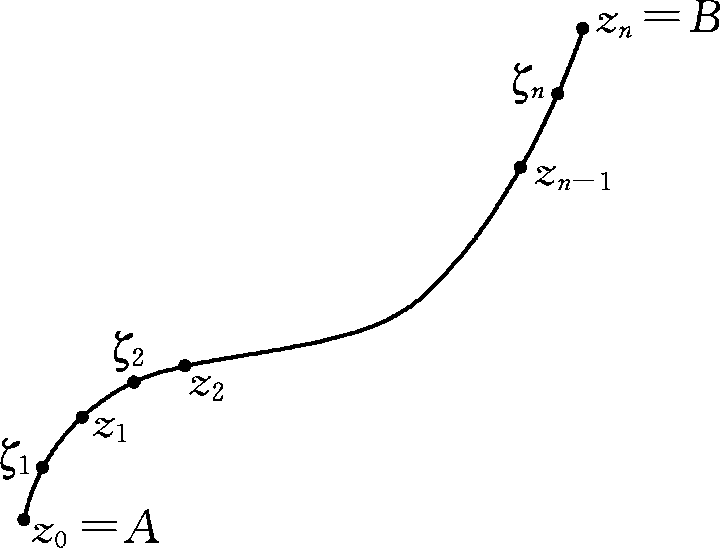
\includegraphics[keepaspectratio,alt={图3.1 曲线 C 的划分与积分和 S\_n}]{figures/03-复变函数的积分/fig-p03-6054f883.png}}
\caption{图3.1 曲线 \(C\) 的划分与积分和 \(S_n\)}
\end{figure}

\subsection{3.1.2
闭曲线上的积分与正方向}\label{ux95edux66f2ux7ebfux4e0aux7684ux79efux5206ux4e0eux6b63ux65b9ux5411}

若 \(C\) 为闭曲线，\(C\) 的正方向指的是：当点沿着曲线 \(C\)
按所选定取积分的方向运动时，\(C\) 所围区域始终在它的左侧。这时函数
\(f(z)\) 沿曲线 \(C\) 的积分记作

\[
\oint_C f(z)\,dz .
\]

\subsection{3.1.3
复变函数积分的性质}\label{ux590dux53d8ux51fdux6570ux79efux5206ux7684ux6027ux8d28}

\textbf{性质 3.1（方向性）} 若函数 \(f(z)\) 沿曲线 \(C\) 可积，则

\[
\int_C f(z)\,dz=-\int_{C^-} f(z)\,dz .
\]

\textbf{性质 3.2（线性性）} 若函数 \(f(z)\) 和 \(g(z)\) 沿曲线 \(C\)
可积，则

\[
\int_C\big[\alpha f(z)+\beta g(z)\big]\,dz
=\alpha\int_C f(z)\,dz+\beta\int_C g(z)\,dz,
\]

其中 \(\alpha,\beta\) 为任意常数。

\textbf{性质 3.3（对积分路径的可加性）} 若函数 \(f(z)\) 沿曲线 \(C\)
可积，曲线 \(C\) 由曲线段 \(C_1,C_2,\dots,C_n\) 依次首尾相接而成，则

\[
\int_C f(z)\,dz=\int_{C_1}f(z)\,dz+\int_{C_2}f(z)\,dz+\cdots+\int_{C_n}f(z)\,dz .
\]

\textbf{性质 3.4（积分不等式）} 若函数 \(f(z)\) 沿曲线 \(C\) 可积，且对
\(\forall z\in C\) 满足 \(|f(z)|\le M\)，曲线 \(C\) 的长度为 \(L\)，则

\[
\left|\int_C f(z)\,dz\right|\le\int_C |f(z)|\,ds\le ML,
\]

其中 \(ds=|dz|=\sqrt{dx^2+dy^2}\) 为曲线 \(C\) 的\textbf{弧微分}。

\textbf{证明要点} 记 \(\Delta s_k\) 为 \(z_{k-1}\) 与 \(z_k\)
之间的弧长，则

\[
\left|\sum_{k=1}^{n}f(\zeta_k)\Delta z_k\right|
\le\sum_{k=1}^{n}|f(\zeta_k)|\,|\Delta z_k|
\le\sum_{k=1}^{n}|f(\zeta_k)|\,\Delta s_k .
\]

令 \(\lambda\to 0\)，两端取极限得

\[
\left|\int_C f(z)\,dz\right|\le\int_C |f(z)|\,ds .
\]

又

\[
\sum_{k=1}^{n}|f(\zeta_k)|\,\Delta s_k\le M\sum_{k=1}^{n}\Delta s_k=ML,
\]

故

\[
\left|\int_C f(z)\,dz\right|\le\int_C |f(z)|\,ds\le ML .
\]

\subsection{3.1.4
复变函数积分的基本计算方法}\label{ux590dux53d8ux51fdux6570ux79efux5206ux7684ux57faux672cux8ba1ux7b97ux65b9ux6cd5}

\textbf{定理 3.1} 若函数 \(f(z)=u(x,y)+iv(x,y)\) 沿曲线 \(C\) 连续，则
\(f(z)\) 沿 \(C\) 可积，且

\[
\int_C f(z)\,dz=\int_C u\,dx-v\,dy+i\int_C v\,dx+u\,dy .
\]

\textbf{证明要点} 记 \(z_k=x_k+iy_k\)，\(\zeta_k=\xi_k+i\eta_k\)，则

\[
\Delta x_k=x_k-x_{k-1},\qquad \Delta y_k=y_k-y_{k-1},\qquad \Delta z_k=\Delta x_k+i\Delta y_k .
\]

于是

\[
\begin{aligned}
\sum_{k=1}^{n}f(\zeta_k)\Delta z_k
&=\sum_{k=1}^{n}\bigl(u(\xi_k,\eta_k)+iv(\xi_k,\eta_k)\bigr)(\Delta x_k+i\Delta y_k)\\
&=\sum_{k=1}^{n}\bigl[u(\xi_k,\eta_k)\Delta x_k-v(\xi_k,\eta_k)\Delta y_k\bigr]
+i\sum_{k=1}^{n}\bigl[v(\xi_k,\eta_k)\Delta x_k+u(\xi_k,\eta_k)\Delta y_k\bigr].
\end{aligned}
\]

已知 \(f(z)\) 沿 \(C\) 连续，所以必有 \(u,v\) 都沿 \(C\)
连续，于是这两个第二类曲线积分都存在，因此积分存在，且

\[
\int_C f(z)\,dz=\int_C u\,dx-v\,dy+i\int_C v\,dx+u\,dy .
\]

\textbf{参数方程法} 设 \(C\) 为一光滑或分段光滑曲线，其参数方程为

\[
z=z(t)=x(t)+iy(t)\quad(a\le t\le b),
\]

参数 \(t=a\) 时对应曲线 \(C\) 的起点，\(t=b\) 时对应曲线 \(C\) 的终点。

设 \(f(z)\) 沿曲线 \(C\) 连续，则

\[
f\bigl(z(t)\bigr)=u\bigl(x(t),y(t)\bigr)+iv\bigl(x(t),y(t)\bigr)=u(t)+iv(t),
\]

且

\[
\int_C f(z)\,dz=\int_a^b f\bigl(z(t)\bigr)z'(t)\,dt .
\]

其中

\[
\operatorname{Re}\bigl(f(z(t))z'(t)\bigr)=u(t)x'(t)-v(t)y'(t),
\]

\[
\operatorname{Im}\bigl(f(z(t))z'(t)\bigr)=u(t)y'(t)+v(t)x'(t).
\]

\subsection{3.1.5 典型例题}\label{ux5178ux578bux4f8bux9898}

\textbf{例 3.1} 分别沿下列路径计算积分 \(\int_C z^2\,dz\) 和
\(\int_C\operatorname{Im}(z)\,dz\)：

\begin{enumerate}
\def\labelenumi{\arabic{enumi}.}
\tightlist
\item
  \(C\) 为从原点 \((0,0)\) 到 \((1,1)\) 的直线段；
\item
  \(C\) 为从原点 \((0,0)\) 到 \((1,0)\) 再到 \((1,1)\) 的直线段。
\end{enumerate}

\textbf{解} (1) \(C\) 的参数方程为 \(z=(1+i)t\)，\(t\) 从 \(0\) 到
\(1\)，于是

\[
\int_C z^2\,dz
=\int_0^1\bigl[(1+i)t\bigr]^2 d\bigl((1+i)t\bigr)
=\int_0^1 (1+i)\bigl((1+i)t\bigr)^2dt
=(1+i)^3\int_0^1 t^2dt
=\frac{(1+i)^3}{3}.
\]

同时

\[
\int_C\operatorname{Im}(z)\,dz=\int_0^1 t\,d\bigl((1+i)t\bigr)=(1+i)\int_0^1 t\,dt=\frac{1+i}{2}.
\]

\begin{enumerate}
\def\labelenumi{(\arabic{enumi})}
\setcounter{enumi}{1}
\tightlist
\item
  把从 \((0,0)\) 到 \((1,0)\) 和从 \((1,0)\) 到 \((1,1)\)
  的两直线段分别记为 \(C_1\) 和 \(C_2\)。\(C_1\) 的参数方程为
  \(y=0\)，\(x\) 从 \(0\) 到 \(1\)；\(C_2\) 的参数方程为 \(x=1\)，\(y\)
  从 \(0\) 到 \(1\)。于是
\end{enumerate}

\[
\begin{aligned}
\int_C z^2\,dz
&=\int_{C_1}z^2\,dz+\int_{C_2}z^2\,dz
=\int_0^1 x^2\,dx+\int_0^1(1+iy)^2\,d(1+iy)\\
&=\frac{x^3}{3}\Big|_0^1+i\left(y-\frac{y^3}{3}+iy^2\right)\Big|_0^1
=\frac13+i-\frac{i}{3}-1=\frac{2i-2}{3}=\frac{(1+i)^3}{3},
\end{aligned}
\]

且

\[
\int_C\operatorname{Im}(z)\,dz=\int_0^1 0\,dx+\int_0^1 y\,d(1+iy)=\frac{i}{2}.
\]

\begin{quote}
说明：\(\int_C z^2dz\) 沿两条路径的值相同（因为 \(z^2\)
在复平面解析，积分与路径无关），而 \(\int_C\operatorname{Im}(z)dz\)
沿两条路径的值不同，说明非解析函数的积分一般与路径有关。
\end{quote}

\textbf{例 3.2} 计算积分 \(\oint_C \dfrac{\bar z}{z}\,dz\)，其中 \(C\)
为图 3.2 所示半圆环区域的正向边界。

\begin{figure}
\centering
\pandocbounded{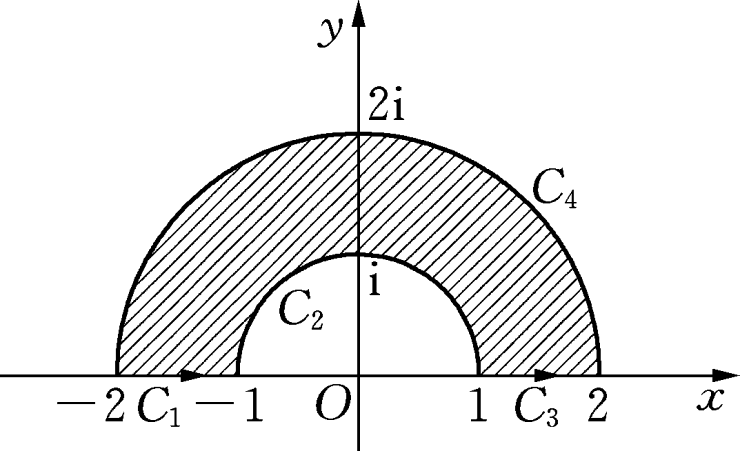
\includegraphics[keepaspectratio,alt={图3.2 半圆环区域及其正向边界}]{figures/03-复变函数的积分/fig-p12-3b3622a3.png}}
\caption{图3.2 半圆环区域及其正向边界}
\end{figure}

\textbf{解}
积分路径可分为四段：\(C_1:z=t\ (-2\le t\le -1)\)；\(C_2:z=e^{i\theta}\)（\(\theta\)
从 \(\pi\) 到
\(0\)）；\(C_3:z=t\ (1\le t\le 2)\)；\(C_4:z=2e^{i\theta}\)（\(\theta\)
从 \(0\) 到 \(\pi\)）。于是

\[
\begin{aligned}
\oint_C\frac{\bar z}{z}\,dz
&=\int_{C_1}\frac{\bar z}{z}\,dz+\int_{C_2}\frac{\bar z}{z}\,dz+\int_{C_3}\frac{\bar z}{z}\,dz+\int_{C_4}\frac{\bar z}{z}\,dz\\
&=\int_{-2}^{-1}\frac{t}{t}\,dt+\int_{\pi}^{0}\frac{e^{i\theta}}{e^{-i\theta}}\,i e^{i\theta}\,d\theta
+\int_{1}^{2}\frac{t}{t}\,dt+\int_{0}^{\pi}\frac{2e^{i\theta}}{2e^{-i\theta}}\,2i e^{i\theta}\,d\theta\\
&=1+\frac23+1-\frac43=\frac43 .
\end{aligned}
\]

\begin{quote}
注：幻灯片对两条圆弧的代入写作
\(\dfrac{e^{i\theta}}{e^{-i\theta}}\)，这对应的是
\(\dfrac{z}{\bar z}\)；若严格按题面 \(\dfrac{\bar z}{z}\)
计算，两条圆弧分别得 \(-2\) 与 \(4\)，总值为
\(4\)。此处按幻灯片原式与结果 \(4/3\) 转写，请以教材/课堂为准。
\end{quote}

\textbf{例 3.3} 计算积分 \(\oint_C\dfrac{dz}{(z-z_0)^{n+1}}\)，其中
\(C\) 为以 \(z_0\) 为中心、\(r\) 为半径的正向圆周，\(n\) 为整数。

\textbf{解} 曲线 \(C\) 的方程为
\(z=z_0+re^{i\theta}\ (0\le\theta\le2\pi)\)，于是

\[
I=\oint_C\frac{dz}{(z-z_0)^{n+1}}
=\int_0^{2\pi}\frac{i r e^{i\theta}d\theta}{r^{n+1}e^{i(n+1)\theta}}
=\int_0^{2\pi}\frac{i}{r^n e^{in\theta}}d\theta
=\frac{i}{r^n}\int_0^{2\pi}e^{-in\theta}d\theta .
\]

当 \(n=0\) 时，

\[
I=i\int_0^{2\pi}d\theta=2\pi i ;
\]

当 \(n\neq0\) 时，

\[
I=\frac{i}{r^n}\int_0^{2\pi}(\cos n\theta-i\sin n\theta)\,d\theta=0 .
\]

因此

\[
\oint_{|z-z_0|=r}\frac{dz}{(z-z_0)^{n+1}}
=\begin{cases}2\pi i, & n=0,\\ 0, & n\neq0.\end{cases}
\]

\begin{figure}
\centering
\pandocbounded{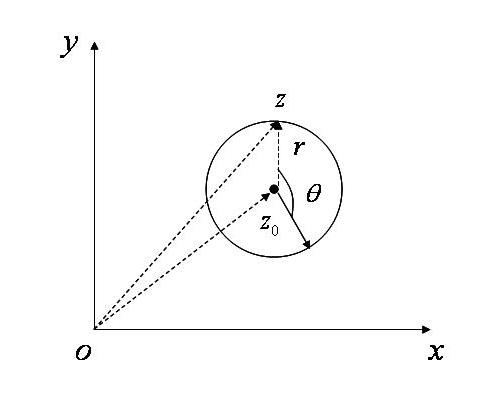
\includegraphics[keepaspectratio,alt={图3.3 以 z\_0 为圆心的正向圆周}]{figures/03-复变函数的积分/fig-p13-8809ed0a.jpg}}
\caption{图3.3 以 \(z_0\) 为圆心的正向圆周}
\end{figure}

\subsection{常见错误与注意点}\label{ux5e38ux89c1ux9519ux8befux4e0eux6ce8ux610fux70b9-7}

\begin{enumerate}
\def\labelenumi{\arabic{enumi}.}
\tightlist
\item
  \textbf{方向约定}：\(\int_C=-\int_{C^-}\)；闭曲线的正向是使其所围区域始终位于左侧的方向（通常取逆时针）。
\item
  \textbf{积分不等式}：左端是``积分模''的不等式，右端用弧长作估计，\(ds=|dz|\)，最终有
  \(ML\)；不要遗漏``总长度 \(L\)''这一因子。
\item
  \textbf{\(\operatorname{Im}(z)\) 的积分}：\(\operatorname{Im}(z)\)
  不是解析函数，其积分一般与路径有关，不能像解析函数那样随意换路径。
\item
  \textbf{例 3.2 的记号}：幻灯片解法的圆弧代入写的是
  \(\dfrac{z}{\bar z}\)（即
  \(\dfrac{e^{i\theta}}{e^{-i\theta}}\)），与题面 \(\dfrac{\bar z}{z}\)
  不一致，注意区分两者的积分值。
\end{enumerate}

\subsection{本节小结}\label{ux672cux8282ux5c0fux7ed3-7}

\begin{itemize}
\tightlist
\item
  \textbf{定义}：\(\int_C f(z)dz=\lim\limits_{\lambda\to0}\sum_{k}f(\zeta_k)\Delta z_k\)，其中
  \(\Delta z_k=z_k-z_{k-1}\)。
\item
  \textbf{性质}：方向性、线性性、路径可加性、积分不等式（\(ML\) 估计）。
\item
  \textbf{计算方法}：化归为两个第二类曲线积分，或参数方程法
  \(\int_C f(z)dz=\int_a^b f(z(t))z'(t)dt\)。
\item
  \textbf{重要结果}：\(\oint_{|z-z_0|=r}\dfrac{dz}{(z-z_0)^{n+1}}=\begin{cases}2\pi i,& n=0,\\0,& n\ne0.\end{cases}\)
\end{itemize}

\section{3.2
柯西-古萨定理及其推广}\label{ux67efux897f-ux53e4ux8428ux5b9aux7406ux53caux5176ux63a8ux5e7f}

\begin{quote}
本节目标：理解并掌握柯西-古萨定理及其推论，理解单连通域内``积分与路径无关''的本质，掌握原函数、变上限函数与牛顿-莱布尼茨型公式，并能运用复合闭路定理处理多连通区域上有奇点时的积分。
重点：柯西-古萨定理（\(\oint_C f(z)dz=0\)）、推论 3.1/3.2、原函数与定理
3.3/3.4、复合闭路定理（定理 3.5）及应用。
难点：格林公式与柯西-黎曼方程在证明中的作用；多连通区域与复闭路；奇点与复合闭路选取。
\end{quote}

\subsection{3.2.1
柯西-古萨（Cauchy-Goursat）定理}\label{ux67efux897f-ux53e4ux8428cauchy-goursatux5b9aux7406}

假设函数 \(f(z)=u+iv\) 在单连通域 \(D\) 内处处解析，\(f'(z)\) 在 \(D\)
内连续，\(u,v\) 对 \(x,y\) 的偏导数在 \(D\) 内连续。设 \(z=x+iy\)，\(C\)
为 \(D\) 内任一条简单闭曲线。由定理 3.1 有

\[
\int_C f(z)\,dz=\int_C u\,dx-v\,dy+i\int_C v\,dx+u\,dy .
\]

记 \(G\) 为 \(C\) 所围区域，由格林（Green）公式有

\[
\int_C u\,dx-v\,dy=\iint_G\left(-\frac{\partial v}{\partial x}-\frac{\partial u}{\partial y}\right)dxdy .
\]

由于 \(f(z)=u+iv\) 在 \(D\) 内解析，所以 \(u,v\) 在 \(D\)
内处处满足柯西-黎曼方程，即

\[
\frac{\partial u}{\partial x}=\frac{\partial v}{\partial y},\qquad \frac{\partial v}{\partial x}=-\frac{\partial u}{\partial y}.
\]

因此

\[
\int_C u\,dx-v\,dy=\int_C v\,dx-u\,dy=0,
\]

从而

\[
\oint_C f(z)\,dz=0 .
\]

\textbf{定理 3.2（柯西-古萨定理）} 若函数 \(f(z)\) 是单连通域 \(D\)
内的解析函数，则 \(f(z)\) 沿 \(D\) 内任一条闭曲线 \(C\) 的积分为零，即

\[
\oint_C f(z)\,dz=0 .
\]

任意一条闭曲线都可以看成是由有限多条简单闭曲线衔接而成的。

\begin{figure}
\centering
\pandocbounded{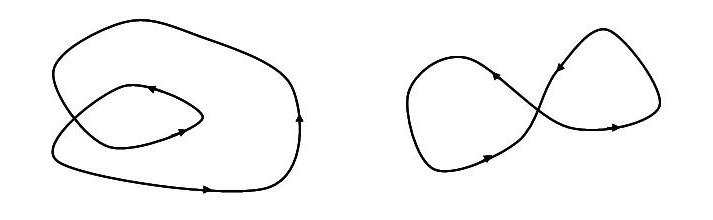
\includegraphics[keepaspectratio,alt={图3.4 闭曲线分解为有限多条简单闭曲线}]{figures/03-复变函数的积分/fig-p15-c94f538e.jpg}}
\caption{图3.4 闭曲线分解为有限多条简单闭曲线}
\end{figure}

\subsection{3.2.2
柯西-古萨定理的推论}\label{ux67efux897f-ux53e4ux8428ux5b9aux7406ux7684ux63a8ux8bba}

\textbf{推论 3.1} 设 \(C\) 为 \(z\) 平面上的一条闭曲线，它围成单连通域
\(D\)，若函数 \(f(z)\) 在 \(\bar D=D\cup C\) 上解析，则

\[
\oint_C f(z)\,dz=0 .
\]

\textbf{推论 3.2} 设函数 \(f(z)\) 在单连通域 \(D\) 解析，则 \(f(z)\) 在
\(D\) 内积分与路径无关。即积分 \(\int_C f(z)dz\) 不依赖于连接起点
\(z_0\) 与终点 \(z_1\) 的曲线 \(C\)，而只与 \(z_0\)、\(z_1\)
的位置有关。

\textbf{证明要点} 设 \(C_1\) 和 \(C_2\) 为 \(D\) 内连接 \(z_0\) 与
\(z_1\) 的任意两条曲线。显然 \(C_1\) 与 \(C_2^-\) 连接成 \(D\)
内一条闭曲线 \(C\)。由柯西-古萨定理

\[
\int_{C_1}f(z)\,dz+\int_{C_2^-}f(z)\,dz=\oint_C f(z)\,dz=0 .
\]

故

\[
\int_{C_1}f(z)\,dz=\int_{C_2}f(z)\,dz .
\]

\begin{figure}
\centering
\pandocbounded{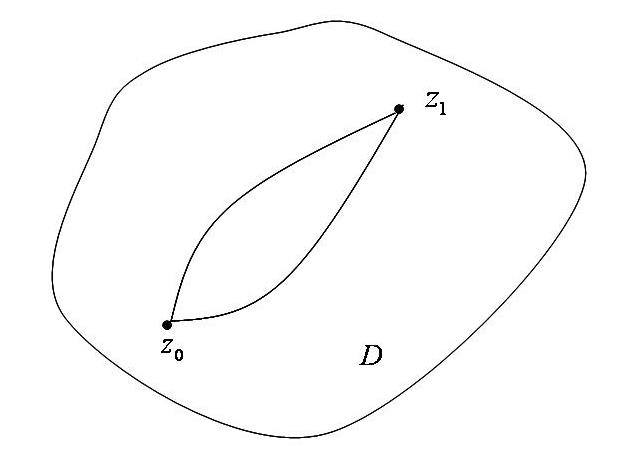
\includegraphics[keepaspectratio,alt={图3.5 积分与路径无关}]{figures/03-复变函数的积分/fig-p16-23ad9722.jpg}}
\caption{图3.5 积分与路径无关}
\end{figure}

\subsection{3.2.3 原函数}\label{ux539fux51fdux6570}

函数 \(f(z)\) 沿曲线 \(C_1\) 和 \(C_2\) 的积分又可以表示为

\[
\int_{C_1}f(z)\,dz=\int_{C_2}f(z)\,dz=\int_{z_0}^{z_1}f(z)\,dz .
\]

固定下限 \(z_0\)，让上限 \(z_1\) 在区域 \(D\) 内变动，并令
\(z_1=z\)，则确定了一个关于上限 \(z\) 的单值函数

\[
F(z)=\int_{z_0}^{z}f(\zeta)\,d\zeta .
\]

并称 \(F(z)\) 为定义在区域 \(D\)
内的\textbf{积分上限函数}或\textbf{变上限函数}。

\textbf{定理 3.3} 若函数 \(f(z)\) 在单连通域 \(D\) 内解析，则函数
\(F(z)\) 必在 \(D\) 内解析，且 \(F'(z)=f(z)\)。

\textbf{证明要点} 若 \(D\) 内任取一点 \(z\)，以 \(z\) 为中心作一个含于
\(D\) 内的小圆 \(B\)，在 \(B\) 内取点
\(z+\Delta z\)（\(\Delta z\neq0\)）。由积分与路径无关，

\[
F(z+\Delta z)-F(z)=\int_{z_0}^{z+\Delta z}f(\zeta)\,d\zeta-\int_{z_0}^{z}f(\zeta)\,d\zeta=\int_{z}^{z+\Delta z}f(\zeta)\,d\zeta .
\]

而 \(f(z)\) 是与积分变量 \(\zeta\) 无关的值，故

\[
\int_{z}^{z+\Delta z}f(z)\,d\zeta=f(z)\int_{z}^{z+\Delta z}d\zeta=f(z)\Delta z .
\]

于是

\[
\frac{F(z+\Delta z)-F(z)}{\Delta z}-f(z)
=\frac{1}{\Delta z}\int_{z}^{z+\Delta z}\bigl(f(\zeta)-f(z)\bigr)d\zeta .
\]

又 \(f(z)\) 在 \(D\) 内解析，显然 \(f(z)\) 在 \(D\)
内连续。所以对于任给的 \(\varepsilon>0\)，必存在 \(\delta>0\)，使得当
\(|\zeta-z|<\delta\)（且 \(\zeta\) 落在圆 \(B\) 内），即当
\(|\Delta z|<\delta\) 时，总有 \(|f(\zeta)-f(z)|<\varepsilon\)，从而

\[
\left|\frac{F(z+\Delta z)-F(z)}{\Delta z}-f(z)\right|
\le\frac{1}{|\Delta z|}\int_{z}^{z+\Delta z}|f(\zeta)-f(z)|\,d\zeta
\le\frac{1}{|\Delta z|}\varepsilon|\Delta z|=\varepsilon .
\]

故

\[
\lim_{\Delta z\to0}\frac{F(z+\Delta z)-F(z)}{\Delta z}=f(z),\qquad F'(z)=f(z) .
\]

\begin{figure}
\centering
\pandocbounded{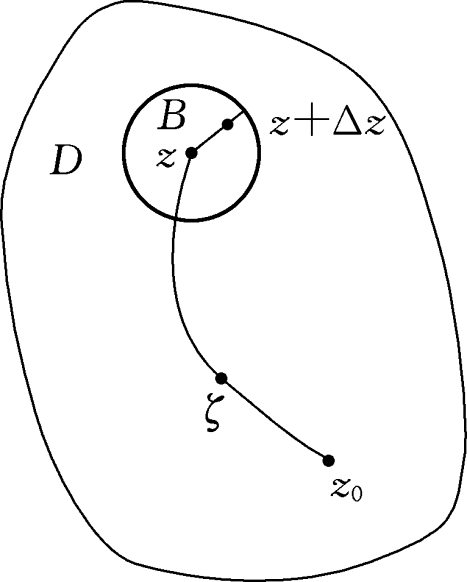
\includegraphics[keepaspectratio,alt={图3.6 定理3.3证明中的小圆 B}]{figures/03-复变函数的积分/fig-p18-e9084205.png}}
\caption{图3.6 定理3.3证明中的小圆 \(B\)}
\end{figure}

\textbf{定义 3.2} 若在区域 \(D\) 内，\(\varphi(z)\) 的导数等于
\(f(z)\)，则称 \(\varphi(z)\) 为 \(f(z)\) 在 \(D\)
内的\textbf{原函数}。变上限函数

\[
F(z)=\int_{z_0}^{z}f(\zeta)\,d\zeta
\]

为 \(f(z)\) 的一个原函数。那么函数 \(f(z)\) 的全体原函数可以表示为

\[
\varphi(z)=F(z)+C,
\]

其中 \(C\) 为任意常数。

\textbf{定理 3.4} 若函数 \(f(z)\) 在单连通域 \(D\)
内处处解析，\(\varphi(z)\) 为 \(f(z)\) 的一个原函数，则

\[
\int_{z_0}^{z_1}f(z)\,dz=\varphi(z_1)-\varphi(z_0)=\varphi(z)\Big|_{z_0}^{z_1},
\]

其中 \(z_0\)、\(z_1\) 为 \(D\) 内的点。

\textbf{证明要点} \(F(z)=\int_{z_0}^{z}f(\zeta)\,d\zeta\) 为 \(f(z)\)
的一个原函数，故

\[
F(z)=\int_{z_0}^{z}f(\zeta)\,d\zeta=\varphi(z)+C .
\]

当 \(z=z_0\) 时，根据柯西-古萨定理可知

\[
\int_{z_0}^{z_0}f(\zeta)\,d\zeta=\varphi(z_0)-\varphi(z_0)=0 .
\]

于是 \(C=-\varphi(z_0)\)，故

\[
\int_{z_0}^{z_1}f(z)\,dz=\varphi(z_1)-\varphi(z_0) .
\]

\textbf{例 3.4} 求积分 \(\displaystyle\int_0^{\pi i/2}\sin 2z\,dz\)
的值。

\textbf{解} 因为 \(\sin 2z\) 在复平面上解析，所以积分与路径无关。

\[
\int_0^{\pi i/2}\sin 2z\,dz
=-\frac12\cos 2z\Big|_0^{\pi i/2}
=-\frac12(\cos\pi i-\cos0)
=-\frac12\left(\frac{e^{-\pi}+e^{\pi}}{2}-1\right)
=\frac12-\frac{e^{-\pi}+e^{\pi}}{4}.
\]

\textbf{例 3.5} 求积分 \(\displaystyle\int_0^i(z-1)e^{-z}\,dz\) 的值。

\textbf{解} 因为 \((z-1)e^{-z}\) 在复平面上解析，所以积分与路径无关。

\[
\int_0^i(z-1)e^{-z}\,dz=\int_0^i ze^{-z}\,dz-\int_0^i e^{-z}\,dz .
\]

上式右边第一个积分采用分部积分法，第二个积分可用凑微分法：

\[
\int_0^i(z-1)e^{-z}\,dz
=-ze^{-z}\Big|_0^i+\int_0^i e^{-z}\,dz-\int_0^i e^{-z}\,dz
=-ie^{-i}=-\sin1-i\cos1 .
\]

\subsection{3.2.4
复合闭路定理}\label{ux590dux5408ux95edux8defux5b9aux7406}

设有 \(n+1\) 条简单闭曲线 \(C_0,C_1,C_2,\dots,C_n\)，其中
\(C_1,C_2,\dots,C_n\) 互不相交也互不包含，并且都含于 \(C_0\) 的内部。这
\(n+1\) 条曲线围成了一个多连通区域 \(D\)，\(D\) 的边界 \(C\)
称作\textbf{复闭路}，它的正向为 \(C_0\)
取逆时针方向，其它曲线都取顺时针方向。因此复闭路记作

\[
C=C_0+C_1^-+C_2^-+\cdots+C_n^- .
\]

\textbf{定理 3.5} 若 \(f(z)\) 在复闭路
\(C=C_0+C_1^-+C_2^-+\cdots+C_n^-\) 及其所围成的多连通区域内解析，则

\[
\oint_{C_0}f(z)\,dz=\oint_{C_1}f(z)\,dz+\oint_{C_2}f(z)\,dz+\cdots+\oint_{C_n}f(z)\,dz ,
\]

也就是

\[
\oint_C f(z)\,dz=0 .
\]

\textbf{证明要点} 做辅助线 \(l_1,l_2,l_3\) 将 \(C_0\)、\(C_1\) 及
\(C_2\) 连接起来，从而把多连通区域 \(D\) 划分为两个单连通区域 \(D_1\) 及
\(D_2\)，并分别用 \(\Gamma_1\) 及 \(\Gamma_2\)
表示这两个区域的边界。由柯西-古萨定理

\[
\oint_{\Gamma_1}f(z)\,dz=0,\qquad \oint_{\Gamma_2}f(z)\,dz=0 .
\]

两式相加，辅助线上的积分正负相抵，得

\[
\oint_{C_0}f(z)\,dz-\oint_{C_1}f(z)\,dz-\oint_{C_2}f(z)\,dz=0,
\]

故

\[
\oint_{C_0}f(z)\,dz=\oint_{C_1}f(z)\,dz+\oint_{C_2}f(z)\,dz .
\]

\begin{figure}
\centering
\pandocbounded{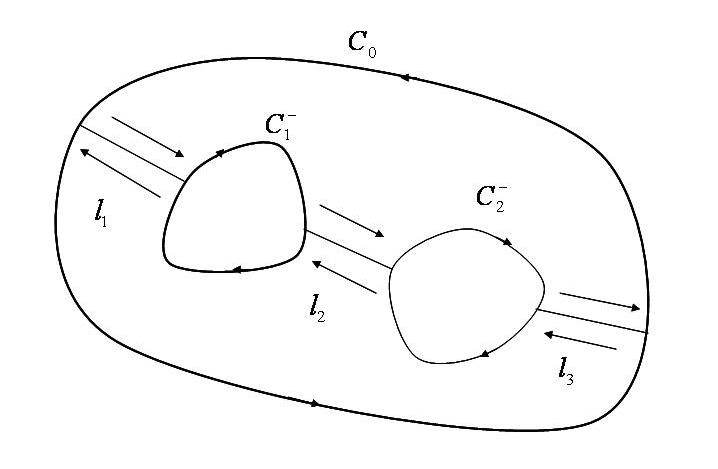
\includegraphics[keepaspectratio,alt={图3.7 复合闭路定理的证明}]{figures/03-复变函数的积分/fig-p25-f1470cb5.jpg}}
\caption{图3.7 复合闭路定理的证明}
\end{figure}

\textbf{例 3.6} 计算 \(\oint_C\dfrac{dz}{z^2+z}\) 的值，\(C\) 为包含圆周
\(|z|=1\) 在内的任何正向简单闭曲线。

\textbf{解} 显然 \(z=0\) 和 \(z=-1\) 是函数 \(\dfrac{1}{z^2+z}\)
的两个奇点。由于 \(C\) 为包含圆周 \(|z|=1\)
在内的任何正向简单闭曲线，因此也包含了这两个奇点。在 \(C\)
的内部作两个互不包含、互不相交的正向圆周 \(C_1\) 和 \(C_2\)，其中
\(C_1\) 的内部只包含奇点 \(z=-1\)，\(C_2\) 的内部只包含奇点
\(z=0\)。函数 \(\dfrac{1}{z^2+z}\) 在由 \(C\)、\(C_1\)、\(C_2\)
所围成的多连通域内解析，由复合闭路定理及例 3.3，

\[
\begin{aligned}
\oint_C\frac{dz}{z^2+z}
&=\oint_{C_1}\frac{dz}{z^2+z}+\oint_{C_2}\frac{dz}{z^2+z}\\
&=\oint_{C_1}\left(\frac{1}{z}-\frac{1}{z+1}\right)dz
+\oint_{C_2}\left(\frac{1}{z}-\frac{1}{z+1}\right)dz\\
&=0-2\pi i+2\pi i-0=0 .
\end{aligned}
\]

\subsection{常见错误与注意点}\label{ux5e38ux89c1ux9519ux8befux4e0eux6ce8ux610fux70b9-8}

\begin{enumerate}
\def\labelenumi{\arabic{enumi}.}
\tightlist
\item
  \textbf{单连通域是前提}：\(f(z)\) 必须是单连通域 \(D\)
  内的解析函数，才能保证
  \(\oint_C f(z)dz=0\)；若闭曲线内部有奇点，不能直接用柯西-古萨定理。
\item
  \textbf{方向}：复合闭路中外边界 \(C_0\) 取逆时针，内边界 \(C_i\)
  取顺时针；符号不能写反。
\item
  \textbf{原函数存在性}：只有在单连通域内解析的函数才处处有原函数；在非单连通域内变上限函数可能不解析（多值）。
\item
  \textbf{牛顿-莱布尼茨公式}：\(\int_{z_0}^{z_1}f(z)dz=\varphi(z_1)-\varphi(z_0)\)
  的前提是 \(f\) 在单连通域内解析且 \(\varphi\) 是其一原函数。
\item
  \textbf{例 3.6}：要先把 \(\dfrac{1}{z^2+z}\) 拆成
  \(\dfrac1z-\dfrac1{z+1}\)，再分别对每个奇点使用例 3.3 的结论。
\end{enumerate}

\subsection{本节小结}\label{ux672cux8282ux5c0fux7ed3-8}

\begin{itemize}
\tightlist
\item
  \textbf{柯西-古萨定理}：单连通域内解析函数沿闭曲线积分为零。
\item
  \textbf{推论}：\(f\) 在 \(\bar D=D\cup C\) 上解析
  \(\Rightarrow\oint_C fdz=0\)；单连通域内积分与路径无关。
\item
  \textbf{原函数}：变上限函数 \(F(z)=\int_{z_0}^z f(\zeta)d\zeta\)
  解析且 \(F'(z)=f(z)\)；一般原函数 \(\varphi(z)=F(z)+C\)。
\item
  \textbf{定理 3.4}：\(\int_{z_0}^{z_1}fdz=\varphi(z_1)-\varphi(z_0)\)。
\item
  \textbf{复合闭路定理}：多连通区域上
  \(\oint_{C_0}fdz=\sum\oint_{C_i}fdz\)（内边界取顺时针）。
\end{itemize}

\section{3.3
柯西积分公式及其推论}\label{ux67efux897fux79efux5206ux516cux5f0fux53caux5176ux63a8ux8bba}

\begin{quote}
本节目标：掌握柯西积分公式及其证明思想，理解解析函数的高阶导数公式与解析函数无穷次可导的性质，能灵活运用柯西积分公式与高阶导数公式计算闭路积分；了解平均值定理。
重点：柯西积分公式、高阶导数公式、定理
3.8/3.9，及其在计算闭路积分中的应用（例 3.7--3.10）。
难点：柯西积分公式的证明（复合闭路、\(r\to0\)
估计）；高阶导数公式中的``导数阶数''与``极点阶数''匹配；含多个奇点时的拆分。
\end{quote}

\subsection{3.3.1
柯西（Cauchy）积分公式}\label{ux67efux897fcauchyux79efux5206ux516cux5f0f}

\textbf{定理 3.6} 若 \(f(z)\) 是区域 \(D\) 内的解析函数，\(C\) 为 \(D\)
内的简单闭曲线，\(C\) 所围内部全含于 \(D\) 内，\(z\) 为 \(C\)
内部任一点，则

\[
f(z)=\frac{1}{2\pi i}\oint_C\frac{f(\zeta)}{\zeta-z}\,d\zeta,
\]

其中积分沿曲线 \(C\) 的正向。上式称为\textbf{柯西积分公式}。

\textbf{证明要点} 取定 \(C\) 内部一点 \(z\)。因为 \(f(z)\) 在 \(D\)
内解析，所以 \(f(z)\) 在点 \(z\) 连续，即对任给的
\(\forall\varepsilon>0\)，必存在 \(\delta>0\)，当 \(|\zeta-z|<\delta\)
时，有 \(|f(\zeta)-f(z)|<\varepsilon\)。

令

\[
F(\zeta)=\frac{f(\zeta)}{\zeta-z},
\]

则 \(F(\zeta)\) 在 \(D\) 内除去点 \(z\) 外处处解析。现以 \(z\)
为中心、\(r\) 为半径作圆周

\[
B:|\zeta-z|=r,
\]

使圆 \(B\) 的内部及边界全含于 \(C\) 的内部。由复合闭路定理有

\[
\oint_C\frac{f(\zeta)}{\zeta-z}\,d\zeta=\oint_B\frac{f(\zeta)}{\zeta-z}\,d\zeta .
\]

令 \(r\to0\)，只需证明

\[
\oint_B\frac{f(\zeta)}{\zeta-z}\,d\zeta\to2\pi i f(z) .
\]

因为

\[
\oint_B\frac{1}{\zeta-z}\,d\zeta=2\pi i ,
\]

而 \(f(z)\) 与 \(\zeta\) 无关，于是

\[
\begin{aligned}
\left|\oint_B\frac{f(\zeta)}{\zeta-z}\,d\zeta-2\pi i f(z)\right|
&=\left|\oint_B\frac{f(\zeta)-f(z)}{\zeta-z}\,d\zeta\right|\\
&\le\oint_B\frac{|f(\zeta)-f(z)|}{|\zeta-z|}\,|d\zeta|
\le\oint_B\frac{\varepsilon}{r}\,ds
=\frac{\varepsilon}{r}\cdot2\pi r=2\pi\varepsilon .
\end{aligned}
\]

当 \(r\to0\)（从而
\(\zeta\to z\)）时，\(2\pi\varepsilon\to0\)，故柯西积分公式成立。

\begin{figure}
\centering
\pandocbounded{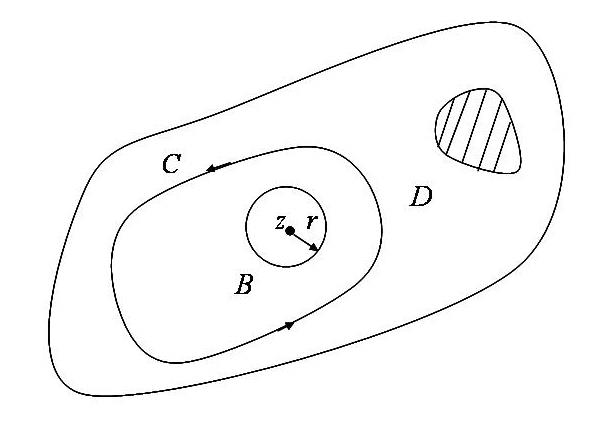
\includegraphics[keepaspectratio,alt={图3.8 柯西积分公式证明中的圆周 B}]{figures/03-复变函数的积分/fig-p28-7facc483.jpg}}
\caption{图3.8 柯西积分公式证明中的圆周 \(B\)}
\end{figure}

\textbf{平均值定理} 若函数 \(f(z)\) 在曲线 \(C\) 上恒为常数
\(K\)，\(z_0\) 为 \(C\) 内部任一点，则由柯西积分公式

\[
f(z)=\frac{1}{2\pi i}\oint_C\frac{f(\zeta)}{\zeta-z_0}\,d\zeta
=\frac{K}{2\pi i}\oint_C\frac{1}{\zeta-z_0}\,d\zeta
=\frac{K}{2\pi i}\cdot2\pi i=K,
\]

即 \(f(z)\) 在曲线 \(C\) 的内部也恒为常数 \(K\)。

若 \(C\) 为圆周 \(|\zeta-z_0|=R\)，即

\[
\zeta=z_0+Re^{i\theta}\quad(0\le\theta\le2\pi),
\]

则 \(d\zeta=iRe^{i\theta}d\theta\)，从而

\[
f(z_0)=\frac{1}{2\pi i}\oint_C\frac{f(\zeta)}{\zeta-z_0}\,d\zeta
=\frac{1}{2\pi}\int_0^{2\pi}f(z_0+Re^{i\theta})\,d\theta .
\]

\textbf{解析函数在圆心 \(z_0\)
处的值等于它在圆周上的平均值，这就是解析函数的平均值定理。}

若 \(f(z)\) 在简单闭曲线 \(C\) 所围成的区域内解析，且在 \(C\)
上连续，则柯西积分公式仍然成立。柯西积分公式可以改写成

\[
\oint_C\frac{f(\zeta)}{\zeta-z}\,d\zeta=2\pi i f(z) .
\]

\subsection{3.3.2
柯西积分公式的应用}\label{ux67efux897fux79efux5206ux516cux5f0fux7684ux5e94ux7528}

\textbf{例 3.7} 计算积分 \(\oint_{|z|=2}\dfrac{z^2+1}{z}\,dz\) 的值。

\textbf{解} 因为 \(z^2+1\) 在 \(|z|=2\) 内解析，

\[
\oint_{|z|=2}\frac{z^2+1}{z}\,dz
=2\pi i\cdot(z^2+1)\big|_{z=0}=2\pi i .
\]

\textbf{例 3.8} 计算积分
\(\oint_C\dfrac{\sin\frac{\pi z}{6}}{z^2-1}\,dz\) 的值，其中 \(C\) 为：

\begin{enumerate}
\def\labelenumi{\arabic{enumi}.}
\tightlist
\item
  \(|z-\frac32|=1\)；
\item
  \(|z+\frac32|=1\)；
\item
  \(|z|=3\)。
\end{enumerate}

\textbf{解} (1) 被积函数 \(\dfrac{\sin\frac{\pi z}{6}}{z+1}\) 在
\(|z-\frac32|=1\) 的内部解析，故

\[
\oint_C\frac{\sin\frac{\pi z}{6}}{z^2-1}\,dz
=\oint_C\frac{\sin\frac{\pi z}{6}}{z+1}\cdot\frac{1}{z-1}\,dz
=2\pi i\left(\frac{\sin\frac{\pi z}{6}}{z+1}\right)\Big|_{z=1}
=2\pi i\cdot\frac14=\frac{\pi i}{2}.
\]

\begin{enumerate}
\def\labelenumi{(\arabic{enumi})}
\setcounter{enumi}{1}
\tightlist
\item
  被积函数 \(\dfrac{\sin\frac{\pi z}{6}}{z-1}\) 在 \(|z+\frac32|=1\)
  的内部解析，故
\end{enumerate}

\[
\oint_C\frac{\sin\frac{\pi z}{6}}{z^2-1}\,dz
=\oint_C\frac{\sin\frac{\pi z}{6}}{z-1}\cdot\frac{1}{z+1}\,dz
=2\pi i\left(\frac{\sin\frac{\pi z}{6}}{z-1}\right)\Big|_{z=-1}
=2\pi i\cdot\frac14=\frac{\pi i}{2}.
\]

\begin{enumerate}
\def\labelenumi{(\arabic{enumi})}
\setcounter{enumi}{2}
\tightlist
\item
  被积函数在 \(|z|=3\) 的内部有两个奇点 \(z=1\) 和 \(z=-1\)。在 \(C\)
  的内部作两个互不包含、互不相交的正向圆周 \(C_1\) 和 \(C_2\)，其中
  \(C_1\) 的内部只包含奇点 \(z=1\)，\(C_2\) 的内部只包含奇点
  \(z=-1\)。由复合闭路定理及柯西积分公式，
\end{enumerate}

\[
\oint_C\frac{\sin\frac{\pi z}{6}}{z^2-1}\,dz
=\oint_{C_1}\frac{\sin\frac{\pi z}{6}}{z^2-1}\,dz+\oint_{C_2}\frac{\sin\frac{\pi z}{6}}{z^2-1}\,dz
=\frac{\pi i}{2}+\frac{\pi i}{2}=\pi i .
\]

\subsection{3.3.3
高阶导数公式}\label{ux9ad8ux9636ux5bfcux6570ux516cux5f0f}

\textbf{定理 3.7} 定义在区域 \(D\) 的解析函数 \(f(z)\) 有各阶导数，且有

\[
f^{(n)}(z)=\frac{n!}{2\pi i}\oint_C\frac{f(\zeta)}{(\zeta-z)^{n+1}}\,d\zeta\quad(n=1,2,\cdots),
\]

其中 \(C\) 为区域 \(D\) 内围绕 \(z\) 的任何一条简单闭曲线，积分沿曲线
\(C\) 的正向。

\textbf{定理 3.8} 若 \(f(z)\) 为定义在区域 \(D\) 内的解析函数，则在
\(D\)
内其各阶导数都存在并且解析。换句话说，\textbf{解析函数的导数也是解析函数}。

\textbf{定理 3.9} 函数 \(f(z)=u(x,y)+iv(x,y)\) 在区域 \(D\)
内解析的充要条件是：

\begin{enumerate}
\def\labelenumi{\arabic{enumi}.}
\tightlist
\item
  \(u_x,u_y,v_x,v_y\) 在 \(D\) 内连续；
\item
  \(u(x,y),v(x,y)\) 在 \(D\) 内满足柯西-黎曼方程
\end{enumerate}

\[
\frac{\partial u}{\partial x}=\frac{\partial v}{\partial y},\qquad \frac{\partial u}{\partial y}=-\frac{\partial v}{\partial x}.
\]

\textbf{例 3.9} 求积分
\(\oint_C\dfrac{e^z}{\left(z-\dfrac{\pi i}{2}\right)^2}\,dz\) 的值，其中
\(C\) 为 \(x^2+y^2=6y\)。

\textbf{解} 被积函数在 \(C\) 的内部有一个奇点
\(z=\dfrac{\pi i}{2}\)。由高阶导数公式（\(n=1\)），

\[
\oint_C\frac{e^z}{\left(z-\frac{\pi i}{2}\right)^2}\,dz
=2\pi i\left(e^z\right)'\Big|_{z=\pi i/2}
=2\pi i\,e^{\pi i/2}=2\pi i\cdot i=-2\pi .
\]

\textbf{例 3.10} 求积分 \(\oint_C\dfrac{\cos\pi z}{z^3(z-1)^2}\,dz\)
的值，其中 \(C\) 为 \(|z|=2\)。

\textbf{解} 被积函数在 \(C\) 的内部有两个奇点 \(z=0\) 和
\(z=1\)。作两条互不相交且互不包含的闭曲线 \(C_1\) 和
\(C_2\)，分别包围奇点 \(z=0\) 和 \(z=1\)，且两曲线所围区域全含于 \(C\)
的内部。由复合闭路定理和高阶导数公式，

\[
\begin{aligned}
\oint_C\frac{\cos\pi z}{z^3(z-1)^2}\,dz
&=\oint_{C_1}\frac{\cos\pi z}{(z-1)^2}\cdot\frac{1}{z^3}\,dz
+\oint_{C_2}\frac{\cos\pi z}{z^3}\cdot\frac{1}{(z-1)^2}\,dz\\
&=\frac{2\pi i}{2!}\left(\frac{\cos\pi z}{(z-1)^2}\right)''\Big|_{z=0}
+2\pi i\left(\frac{\cos\pi z}{z^3}\right)'\Big|_{z=1}\\
&=(6-\pi^2)\pi i+6\pi i=(12-\pi^2)\pi i .
\end{aligned}
\]

\begin{quote}
说明：幻灯片把第二个导数项记作
\(\left(\dfrac{\cos\pi z}{z^3}\right)'\Big|_{z=0}+2\pi i\cdot3\)，此处按``\(C_2\)
包围 \(z=1\)''的正确理解写为
\(\left(\dfrac{\cos\pi z}{z^3}\right)'\Big|_{z=1}=3\)，从而第二项为
\(2\pi i\cdot3=6\pi i\)。请以正确的求导与求值位置为准。
\end{quote}

\subsection{常见错误与注意点}\label{ux5e38ux89c1ux9519ux8befux4e0eux6ce8ux610fux70b9-9}

\begin{enumerate}
\def\labelenumi{\arabic{enumi}.}
\tightlist
\item
  \textbf{柯西积分公式}：只对``被积函数在 \(C\) 内部解析、\(z\) 在 \(C\)
  内部''的情形使用；要把积分写成 \(\dfrac{f(\zeta)}{\zeta-z}\)
  的形式，其中 \(f(z)\) 在 \(C\) 内部解析。
\item
  \textbf{高阶导数公式}：\(f^{(n)}(z)=\dfrac{n!}{2\pi i}\oint\dfrac{f(\zeta)}{(\zeta-z)^{n+1}}d\zeta\)，注意分母的阶数
  \(n+1\) 与 \(n!\) 的对应；\(n\) 是导数阶数。
\item
  \textbf{例 3.8/3.10}：圆内有多个孤立奇点时，要先``挖孔''作
  \(C_i\)，再用复合闭路分解，最后对每个 \(C_i\)
  用柯西积分公式或高阶导数公式。
\item
  \textbf{证明中的 \(2\pi\varepsilon\)}：幻灯片最后一行写作 \(2\pi i\)
  应为 \(2\pi\varepsilon\)（随 \(r\to0\) 而趋于
  \(0\)），此处已按正确数学含义书写。
\item
  \textbf{\(\sin\frac{\pi z}{6}\) 在 \(z=\pm1\)
  的值}：\(\sin\frac{\pi}{6}=\frac12\)，因此两个单圆积分都等于
  \(\frac{\pi i}{2}\)。
\end{enumerate}

\subsection{本节小结}\label{ux672cux8282ux5c0fux7ed3-9}

\begin{itemize}
\tightlist
\item
  \textbf{柯西积分公式}：\(f(z)=\dfrac{1}{2\pi i}\oint_C\dfrac{f(\zeta)}{\zeta-z}d\zeta\)，等价式
  \(\oint_C\dfrac{f(\zeta)}{\zeta-z}d\zeta=2\pi i f(z)\)。
\item
  \textbf{平均值定理}：解析函数在圆心处的值等于它在圆周上的平均值。
\item
  \textbf{高阶导数公式}：\(f^{(n)}(z)=\dfrac{n!}{2\pi i}\oint_C\dfrac{f(\zeta)}{(\zeta-z)^{n+1}}d\zeta\)，由此得出解析函数无穷次可导且导数仍解析。
\item
  \textbf{解析充要条件}：\(u_x,u_y,v_x,v_y\) 连续且满足柯西-黎曼方程。
\item
  \textbf{应用}：含孤立奇点的闭路积分可通过挖孔 + 柯西积分公式 /
  高阶导数公式计算。
\end{itemize}

\section{3.4
解析函数与调和函数的关系}\label{ux89e3ux6790ux51fdux6570ux4e0eux8c03ux548cux51fdux6570ux7684ux5173ux7cfb}

\begin{quote}
本节目标：理解调和函数与共轭调和函数的概念，掌握``解析函数的实部与虚部都是调和函数''这一结论，并会使用偏积分法、线积分法与不定积分法求已知实部（或虚部）的解析函数及其共轭调和函数。
重点：定义 3.3、定理
3.10、共轭调和函数，以及三种求法（偏积分法、线积分法、不定积分法）。
难点：由柯西-黎曼方程推出调和性；灵活选用恰当方法并把结果整理成解析函数
\(f(z)\) 的表达式。
\end{quote}

\subsection{3.4.1
调和函数与解析函数}\label{ux8c03ux548cux51fdux6570ux4e0eux89e3ux6790ux51fdux6570}

\textbf{定义 3.3} 在区域 \(D\)
内具有二阶连续偏导数并且满足\textbf{拉普拉斯方程}

\[
\frac{\partial^2\varphi}{\partial x^2}+\frac{\partial^2\varphi}{\partial y^2}=0
\]

的二元实函数 \(\varphi(x,y)\) 称为在 \(D\) 内的\textbf{调和函数}。

\textbf{定理 3.10} 任何在区域 \(D\) 内解析的函数
\(f(z)=u(x,y)+iv(x,y)\)，它的实部 \(u(x,y)\) 和虚部 \(v(x,y)\) 都是
\(D\) 内的调和函数。

\textbf{证明要点} 由柯西-黎曼方程有

\[
\frac{\partial u}{\partial x}=\frac{\partial v}{\partial y},\qquad
\frac{\partial u}{\partial y}=-\frac{\partial v}{\partial x}.
\]

对第一式两边关于 \(x\) 求偏导、第二式两边关于 \(y\) 求偏导，得

\[
\frac{\partial^2 u}{\partial x^2}=\frac{\partial^2 v}{\partial y\partial x},\qquad
\frac{\partial^2 u}{\partial y^2}=-\frac{\partial^2 v}{\partial x\partial y}.
\]

由于 \(u(x,y)\) 与 \(v(x,y)\) 具有任意阶连续偏导，所以

\[
\frac{\partial^2 v}{\partial y\partial x}=\frac{\partial^2 v}{\partial x\partial y}.
\]

故

\[
\frac{\partial^2 u}{\partial x^2}+\frac{\partial^2 u}{\partial y^2}=0 .
\]

同理可证

\[
\frac{\partial^2 v}{\partial x^2}+\frac{\partial^2 v}{\partial y^2}=0 .
\]

即 \(u(x,y)\) 与 \(v(x,y)\) 都是调和函数。

\begin{quote}
注：幻灯片第 36 页把第一组柯西-黎曼方程误写为含 \(\varphi\)
的等式，此处按标准柯西-黎曼方程书写。
\end{quote}

使 \(u(x,y)+iv(x,y)\) 在区域 \(D\) 内构成解析函数的调和函数 \(v(x,y)\)
称为 \(u(x,y)\) 的\textbf{共轭调和函数}。或者说，在区域 \(D\)
内满足柯西-黎曼方程

\[
u_x=v_y,\qquad v_x=-u_y
\]

的两个调和函数 \(u\) 和 \(v\) 中，\(v\) 称为 \(u\) 的共轭调和函数。

\subsection{3.4.2
求共轭调和函数的三种方法}\label{ux6c42ux5171ux8f6dux8c03ux548cux51fdux6570ux7684ux4e09ux79cdux65b9ux6cd5}

\subsubsection{3.4.2.1 偏积分法}\label{ux504fux79efux5206ux6cd5}

利用柯西-黎曼方程先求得 \(v\) 对 \(y\) 的偏导 \(v_y=u_x\)，此式关于
\(y\) 积分得

\[
v=\int\frac{\partial u}{\partial x}\,dy+g(x).
\]

然后两边对 \(x\) 求偏导，由 \(v_x=-u_y\)，于是有

\[
-u_y=\frac{\partial}{\partial x}\int\frac{\partial u}{\partial x}\,dy+g'(x).
\]

从而

\[
g(x)=\int\left(-\frac{\partial u}{\partial y}-\frac{\partial}{\partial x}\int\frac{\partial u}{\partial x}\,dy\right)dx+C,
\]

故

\[
v=\int\frac{\partial u}{\partial x}\,dy+\int\left(-\frac{\partial u}{\partial y}-\frac{\partial}{\partial x}\int\frac{\partial u}{\partial x}\,dy\right)dx+C .
\]

\subsubsection{3.4.2.2 线积分法}\label{ux7ebfux79efux5206ux6cd5}

利用柯西-黎曼方程有

\[
dv=v_x dx+v_y dy=-u_y dx+u_x dy .
\]

于是

\[
v=\int_{(x_0,y_0)}^{(x,y)}\bigl(-u_y dx+u_x dy\bigr)+C .
\]

该积分与积分路径无关，因此可选取简单路径（如折线）进行计算，其中
\((x_0,y_0)\) 为区域 \(D\) 中的点。

\subsubsection{3.4.2.3 不定积分法}\label{ux4e0dux5b9aux79efux5206ux6cd5}

根据柯西-黎曼方程及解析函数的导数公式有

\[
f'(z)=u_x+iv_x=u_x-iu_y .
\]

将 \(u_x-iu_y\) 表示成 \(z\) 的函数 \(h(z)\)，于是

\[
f(z)=\int h(z)\,dz+C .
\]

\subsection{3.4.3 典型例题}\label{ux5178ux578bux4f8bux9898-1}

\textbf{例 3.11} 已知
\(u(x,y)=2(x-1)y\)，\(f(2)=-\mathrm{i}\)，求其共轭调和函数，并写出
\(f(z)\) 的形式。

\textbf{解} 由柯西-黎曼方程，有 \(v_y=u_x=2y\)。此式两边关于 \(y\)
积分：

\[
v=\int\frac{\partial u}{\partial x}\,dy+g(x)=y^2+g(x).
\]

于是 \(v_x=g'(x)\)。又由 \(v_x=-u_y=2(1-x)\)，

\[
g(x)=\int2(1-x)\,dx=2x-x^2+C .
\]

故

\[
v=y^2-x^2+2x+C .
\]

因此

\[
f(z)=2(x-1)y+i\bigl(y^2-x^2+2x+C\bigr).
\]

由条件 \(f(2)=-\mathrm{i}\)，得 \(C=-1\)，于是

\[
\begin{aligned}
f(z)&=2(x-1)y+i\bigl(y^2-x^2+2x-1\bigr)\\
&=-i(x^2-y^2+2ixy-2(x+iy)+1)\\
&=-i(z-1)^2 .
\end{aligned}
\]

\textbf{（线积分法说明）} 仍用例 3.11：\(u_x=2y\)，\(u_y=2x-2\)。取
\((x_0,y_0)=(0,0)\)，路径为从 \((0,0)\) 到 \((x,0)\) 的直线段，再从
\((x,0)\) 到 \((x,y)\) 的直线段，则

\[
\begin{aligned}
v&=\int_{(0,0)}^{(x,y)}(-u_y dx+u_x dy)+C\\
&=\int_0^x(2-2x)\,dx+\int_0^y2y\,dy+C
=2x-x^2+y^2+C .
\end{aligned}
\]

\textbf{（不定积分法说明）} 同样对 \(u_x=2y\)，\(u_y=2x-2\)，有

\[
f'(z)=u_x-iu_y=2y-i(2x-2)=-2i(x+iy-1)=-2i(z-1),
\]

故

\[
f(z)=\int-2i(z-1)\,dz+C=-iz^2+2iz+C .
\]

由条件 \(f(2)=-\mathrm{i}\)，得 \(C=-\mathrm{i}\)，故

\[
f(z)=-i(z-1)^2 .
\]

\subsection{常见错误与注意点}\label{ux5e38ux89c1ux9519ux8befux4e0eux6ce8ux610fux70b9-10}

\begin{enumerate}
\def\labelenumi{\arabic{enumi}.}
\tightlist
\item
  \textbf{调和性验证}：只有二阶偏导连续且满足拉普拉斯方程
  \(\varphi_{xx}+\varphi_{yy}=0\)
  的实函数才是调和函数；不能把``解析的实部/虚部''反过来理解为任意调和函数都能构成解析函数（还须满足柯西-黎曼方程）。
\item
  \textbf{共轭调和函数的方向}：\(v\) 是 \(u\) 的共轭调和函数，要求
  \(u_x=v_y,\ v_x=-u_y\)；\(u\) 与 \(v\) 的顺序不能颠倒。
\item
  \textbf{偏积分法}：对 \(y\) 积分得到的``常数''是 \(x\) 的函数
  \(g(x)\)，不要漏掉；最后再代入 \(v_x=-u_y\) 求 \(g(x)\)。
\item
  \textbf{确定常数 \(C\)}：题目若有 \(f(z_0)=w_0\) 的条件，用来定
  \(C\)；无此条件时结果含任意常数。
\item
  \textbf{幻灯片笔误}：第 36 页证明中的柯西-黎曼方程写成含
  \(\varphi\)，第 40 页``用例 3.1 说明''应为``用例 3.11 说明''，第 41
  页``还是用例 3.1 说明''应为``还是用例 3.11
  说明''；本节已按正确写法转写。
\end{enumerate}

\subsection{本节小结}\label{ux672cux8282ux5c0fux7ed3-10}

\begin{itemize}
\tightlist
\item
  \textbf{调和函数}：满足 \(\varphi_{xx}+\varphi_{yy}=0\)
  的二阶连续可导实函数。
\item
  \textbf{定理}：解析函数 \(f=u+iv\) 的实部与虚部都是调和函数；反之，若
  \(u,v\) 满足柯西-黎曼方程则 \(u+iv\) 解析。
\item
  \textbf{共轭调和函数}：\(v\) 是 \(u\) 的共轭调和函数
  \(\iff u_x=v_y,\ v_x=-u_y\)。
\item
  \textbf{三种求法}：偏积分法（先对 \(y\) 积分再定
  \(g(x)\)）、线积分法（与路径无关、取折线）、不定积分法（\(f'(z)=u_x-iu_y\)
  后积分）。
\item
  \textbf{例题模式}：\(u=2(x-1)y,\ f(2)=-i\Rightarrow v=y^2-x^2+2x-1,\ f(z)=-i(z-1)^2\)。
\end{itemize}

\newpage

\chaptercover{4}{解析函数的级数表示法}
%% 由 build/emit_tex.py 生成（生成物，勿手改）；定制请放 user_style.tex / user_meta.yaml
\chapter{第 4 章 ·
解析函数的级数表示法}\label{ux7b2c-4-ux7ae0-ux89e3ux6790ux51fdux6570ux7684ux7ea7ux6570ux8868ux793aux6cd5}

\section{4.1 复数项级数}\label{ux590dux6570ux9879ux7ea7ux6570}

\begin{quote}
本节目标：把实数项级数的极限、收敛、绝对收敛与条件收敛等概念平移到复数域，建立复数列极限与复级数收敛的判定方法。
重点：复数列极限与实、虚部分别收敛的等价关系；复级数收敛的充要条件与必要条件；绝对收敛与条件收敛。
难点：把复级数的收敛性归结为两个实级数；\(\sum a_n\) 收敛与
\(\sum |a_n|\) 收敛的区分。
\end{quote}

对应幻灯片：第 2--10 页。

\subsection{4.1.1
复数列和复数列的极限}\label{ux590dux6570ux5217ux548cux590dux6570ux5217ux7684ux6781ux9650}

\textbf{定义 4.1} 设 \(\{a_n\}(n=1,2,\cdots)\) 为一复数列，其中

\[
a_n=\alpha_n+\mathrm{i}\beta_n,
\]

\(a=\alpha+\mathrm{i}\beta\) 为一确定的复数。如果对任意的正数
\(\varepsilon\)，存在正整数 \(N\)，使得当 \(n>N\) 时，有

\[
|a_n-a|<\varepsilon
\]

成立，则称 \(a\) 为复数列 \(\{a_n\}\) 当 \(n\to\infty\) 时的极限，记作

\[
\lim_{n\to\infty} a_n=a,
\]

并称复数列 \(\{a_n\}\) 收敛于 \(a\)。

\textbf{定理 4.1} 复数列 \(\{a_n\}\) 收敛于 \(a\) 的充分必要条件是

\[
\lim_{n\to\infty}\alpha_n=\alpha,\qquad \lim_{n\to\infty}\beta_n=\beta .
\]

\textbf{证明要点}

\begin{itemize}
\tightlist
\item
  必要性：若 \(\lim a_n=a\)，则对 \(\varepsilon>0\)，存在正整数
  \(N\)，使当 \(n>N\) 时 \(|a_n-a|<\varepsilon\)。从而
\end{itemize}

\[
|\alpha_n-\alpha|\le|a_n-a|<\varepsilon,
\]

故 \(\lim\alpha_n=\alpha\)；同理有 \(\lim\beta_n=\beta\)。

\begin{itemize}
\tightlist
\item
  充分性：若 \(\lim\alpha_n=\alpha\)，\(\lim\beta_n=\beta\)，对
  \(\varepsilon>0\)，存在正整数 \(N\)，使当 \(n>N\) 时
\end{itemize}

\[
|\alpha_n-\alpha|<\frac{\varepsilon}{2},\qquad |\beta_n-\beta|<\frac{\varepsilon}{2},
\]

于是

\[
|a_n-a|\le|\alpha_n-\alpha|+|\beta_n-\beta|<\varepsilon,
\]

故 \(\lim a_n=a\)。

\(\square\)

\subsection{4.1.2 复级数}\label{ux590dux7ea7ux6570}

设 \(\{a_n\}\) 为一复数列，表达式

\[
\sum_{n=1}^{\infty}a_n=a_1+a_2+\cdots+a_n+\cdots
\]

称为复数域上的无穷级数，简称复级数或级数。记该级数的前 \(n\) 项部分和为

\[
s_n=a_1+a_2+\cdots+a_n=\sum_{i=1}^{n}a_i,\qquad (n=1,2,\cdots),
\]

\(\{s_n\}\) 称为该级数的部分和数列。

\textbf{定义 4.2} 若级数 \(\displaystyle\sum_{n=1}^{\infty}a_n\)
对应的部分和数列 \(\{s_n\}\) 收敛于常数 \(s\)，即

\[
\lim_{n\to\infty}s_n=s,
\]

那么 \(\displaystyle\sum_{n=1}^{\infty}a_n\) 称为收敛的级数，数 \(s\)
叫做该级数的和，记为

\[
\sum_{n=1}^{\infty}a_n=s.
\]

若 \(\lim s_n\) 不存在，则称该级数为发散的级数。

\textbf{定理 4.2} 复级数 \(\displaystyle\sum_{n=1}^{\infty}a_n\) 收敛于
\(s\) 的充要条件是实级数 \(\displaystyle\sum_{n=1}^{\infty}\alpha_n\) 和
\(\displaystyle\sum_{n=1}^{\infty}\beta_n\) 分别收敛于 \(\delta\) 和
\(\tau\)，其中

\[
s=\delta+\mathrm{i}\tau,\qquad a_n=\alpha_n+\mathrm{i}\beta_n\ (n=1,2,\cdots).
\]

\textbf{证明要点}

\[
s_n=a_1+a_2+\cdots+a_n=(\alpha_1+\alpha_2+\cdots+\alpha_n)+\mathrm{i}(\beta_1+\beta_2+\cdots+\beta_n)=\delta_n+\mathrm{i}\tau_n,
\]

其中

\[
\delta_n=\sum_{i=1}^{n}\alpha_i,\qquad \tau_n=\sum_{i=1}^{n}\beta_i ,
\]

它们分别为实级数 \(\sum\alpha_i\) 和 \(\sum\beta_i\)（即
\(\sum\alpha_n\)、\(\sum\beta_n\)）的部分和。

由定义 4.2 及定理 4.1 知，\(s_n\) 收敛于 \(s\) 的充要条件是
\(\{\delta_n\}\) 和 \(\{\tau_n\}\) 分别收敛于 \(\delta\) 和
\(\tau\)，从而定理得证。\(\square\)

\textbf{定理 4.3} 复级数 \(\displaystyle\sum_{n=1}^{\infty}a_n\)
收敛的必要条件是

\[
\lim_{n\to\infty}a_n=0 .
\]

\textbf{证明要点} 级数 \(\sum a_n\) 收敛的充要条件是实级数
\(\sum\alpha_n\) 和 \(\sum\beta_n\)
均收敛。实级数收敛的必要条件是其通项的极限为零，即

\[
\lim_{n\to\infty}\alpha_n=0,\qquad \lim_{n\to\infty}\beta_n=0,
\]

从而得到

\[
\lim_{n\to\infty}a_n=0 .
\]

\(\square\)

\textbf{定义 4.3} 对于复级数 \(\displaystyle\sum_{n=1}^{\infty}a_n\)：

\begin{itemize}
\tightlist
\item
  若 \(\displaystyle\sum_{n=1}^{\infty}|a_n|\)
  收敛，则称级数\textbf{绝对收敛}；
\item
  若 \(\displaystyle\sum_{n=1}^{\infty}|a_n|\) 发散，而
  \(\displaystyle\sum_{n=1}^{\infty}a_n\)
  收敛，则称级数\textbf{条件收敛}。
\end{itemize}

\textbf{定理 4.4} 如果级数 \(\displaystyle\sum_{n=1}^{\infty}a_n\)
绝对收敛，则 \(\displaystyle\sum_{n=1}^{\infty}a_n\) 也收敛，且不等式

\[
\left|\sum_{n=1}^{\infty}a_n\right|\le\sum_{n=1}^{\infty}|a_n|
\]

成立。

\textbf{证明要点} 记 \(a_n=\alpha_n+\mathrm{i}\beta_n\)，则

\[
\sum_{n=1}^{\infty}|a_n|=\sum_{n=1}^{\infty}\sqrt{\alpha_n^2+\beta_n^2}.
\]

由于

\[
|\alpha_n|\le\sqrt{\alpha_n^2+\beta_n^2},\qquad |\beta_n|\le\sqrt{\alpha_n^2+\beta_n^2},
\]

所以实级数 \(\sum\alpha_n\) 和 \(\sum\beta_n\) 均收敛，于是 \(\sum a_n\)
收敛。再由部分和取极限并结合三角不等式即得上述不等式。\(\square\)

\textbf{推论 4.1} 设
\(a_n=\alpha_n+\mathrm{i}\beta_n\ (n=1,2,\cdots)\)。则级数
\(\displaystyle\sum_{n=1}^{\infty}a_n\) 绝对收敛的充要条件是级数
\(\displaystyle\sum_{n=1}^{\infty}\alpha_n\) 和
\(\displaystyle\sum_{n=1}^{\infty}\beta_n\) 都绝对收敛。

\subsection{4.1.3 例题}\label{ux4f8bux9898-1}

\textbf{例 4.1} 下列级数是否收敛？是否绝对收敛？

\[
(1)\ \sum_{n=1}^{\infty}\frac{(3\mathrm{i})^n}{n!};\qquad
(2)\ \sum_{n=1}^{\infty}\left(1+\frac{1}{n}\right)\mathrm{e}^{\mathrm{i}\pi/n};\qquad
(3)\ \sum_{n=1}^{\infty}\left[\frac{(-1)^n}{n}+\frac{1}{3^n}\mathrm{i}\right].
\]

\textbf{解}

\textbf{(1)}
\(\left|\dfrac{(3\mathrm{i})^n}{n!}\right|=\dfrac{3^n}{n!}\)。由正项级数的比值判别法知
\(\displaystyle\sum_{n=1}^{\infty}\frac{3^n}{n!}\)
收敛，故原级数为绝对收敛。

\textbf{(2)} 由欧拉公式，

\[
\left(1+\frac{1}{n}\right)\mathrm{e}^{\mathrm{i}\pi/n}=\left(1+\frac{1}{n}\right)\cos\frac{\pi}{n}+\mathrm{i}\left(1+\frac{1}{n}\right)\sin\frac{\pi}{n}.
\]

而

\[
\lim_{n\to\infty}\left(1+\frac{1}{n}\right)\cos\frac{\pi}{n}=1,\qquad
\lim_{n\to\infty}\left(1+\frac{1}{n}\right)\sin\frac{\pi}{n}=0,
\]

所以

\[
\lim_{n\to\infty}\left(1+\frac{1}{n}\right)\mathrm{e}^{\mathrm{i}\pi/n}=1\neq 0 .
\]

故级数
\(\displaystyle\sum_{n=1}^{\infty}\left(1+\frac{1}{n}\right)\mathrm{e}^{\mathrm{i}\pi/n}\)
发散。

\textbf{(3)} 因为 \(\displaystyle\sum_{n=1}^{\infty}\frac{(-1)^n}{n}\)
收敛（且为条件收敛），\(\displaystyle\sum_{n=1}^{\infty}\frac{1}{3^n}\)
也收敛，故原级数收敛。但
\(\displaystyle\sum_{n=1}^{\infty}\left|\frac{(-1)^n}{n}\right|=\sum_{n=1}^{\infty}\frac{1}{n}\)
发散，故原级数为条件收敛。

\subsection{常见错误与注意点}\label{ux5e38ux89c1ux9519ux8befux4e0eux6ce8ux610fux70b9-11}

\begin{itemize}
\tightlist
\item
  不要把``\(\sum a_n\) 收敛''与``\(\sum|a_n|\)
  收敛''混为一谈：前者收敛只能说明通项趋于零，不能保证绝对收敛；\(\sum|a_n|\)
  收敛才保证 \(\sum a_n\) 收敛。
\item
  定理 4.3 只是必要条件：\(\lim a_n=0\) 不能推出 \(\sum a_n\) 收敛。
\item
  判断复级数敛散时，优先把 \(a_n\) 拆成实部 \(\alpha_n\) 与虚部
  \(\beta_n\)，转化为两个实级数来处理。
\item
  例 4.1(2) 属于``通项不趋于零''的情形，是最常用的发散判定。
\end{itemize}

\subsection{本节小结}\label{ux672cux8282ux5c0fux7ed3-11}

\begin{itemize}
\tightlist
\item
  复数列收敛 \(\iff\) 实部、虚部分别收敛（定理
  4.1），从而可用实数极限理论处理复数列。
\item
  复级数由部分和数列 \(\{s_n\}\) 的敛散定义（定义 4.2）；其收敛 \(\iff\)
  实、虚部两个实级数分别收敛（定理 4.2）。
\item
  通项趋于零是复级数收敛的必要条件（定理 4.3）。
\item
  绝对收敛 \(\Rightarrow\) 收敛，且 \(|\sum a_n|\le\sum|a_n|\)（定理
  4.4）；\(\sum a_n\) 绝对收敛 \(\iff\) \(\sum\alpha_n\) 与
  \(\sum\beta_n\) 都绝对收敛（推论 4.1）。
\end{itemize}

\section{4.2 幂级数}\label{ux5e42ux7ea7ux6570}

\begin{quote}
本节目标：掌握幂级数的概念、收敛域（收敛半径、收敛圆）、收敛半径的比值法与根值法，以及幂级数在收敛圆内的解析性（逐项求导、逐项积分）。
重点：收敛半径的两种求法（定理
4.6、4.7）；幂级数在收敛圆内解析、可逐项求导与逐项积分的性质。
难点：收敛半径的意义、\(|z|=R\)
边界上的敛散性、两个幂级数``运算后半径不小于
\(\min\{R_1,R_2\}\)''的理解；幂级数乘法（Cauchy 乘积）的收敛范围。
\end{quote}

对应幻灯片：第 11--24 页。

\subsection{4.2.1
幂级数的概念}\label{ux5e42ux7ea7ux6570ux7684ux6982ux5ff5}

\textbf{幂级数}是指形如

\[
\sum_{n=0}^{\infty} a_n(z-z_0)^n=a_0+a_1(z-z_0)+a_2(z-z_0)^2+\cdots+a_n(z-z_0)^n+\cdots
\]

的表达式，它的一般项是幂函数 \(a_n(z-z_0)^n\)，这里
\(a_n\ (n=0,1,\cdots)\) 和 \(z_0\) 是复常数，而 \(z\) 为复变数。

给定 \(z\) 的一个确定值 \(z_1\)，则

\[
\sum_{n=0}^{\infty}a_n(z_1-z_0)^n=a_0+a_1(z_1-z_0)+a_2(z_1-z_0)^2+\cdots
\]

为复数项级数。若该复数项级数收敛，则称幂级数在 \(z_1\) 处收敛，\(z_1\)
称为幂级数的一个收敛点；否则称为发散点。

若 \(D\) 为幂级数所有收敛点的集合，则级数在 \(D\) 上的和确定一个函数
\(s(z)\)：

\[
s(z)=\sum_{n=0}^{\infty}a_n z^n=a_0+a_1 z+a_2 z^2+\cdots+a_n z^n+\cdots,
\]

称 \(s(z)\) 为幂级数的\textbf{和函数}。特别地，假定
\(z_0=0\)，幂级数成为

\[
\sum_{n=0}^{\infty}a_n z^n=a_0+a_1 z+a_2 z^2+\cdots+a_n z^n+\cdots .
\]

\subsection{4.2.2
收敛半径和收敛圆}\label{ux6536ux655bux534aux5f84ux548cux6536ux655bux5706}

\textbf{定理 4.5} 如果幂级数 \(\displaystyle\sum_{n=0}^{\infty}a_n z^n\)
在 \(z=z_1(\neq 0)\) 处收敛，则对于满足 \(|z|<|z_1|\) 的
\(z\)，级数必绝对收敛；如果在 \(z=z_2\) 处级数发散，则对于 \(|z|>|z_2|\)
的 \(z\)，级数必发散。

\textbf{证明要点} 由于 \(\sum a_n z_1^n\) 级数收敛，有
\(\lim_{n\to\infty}a_n z_1^n=0\)，因而存在正数 \(M\)，使对所有的 \(n\)
成立 \(|a_n z_1^n|<M\)。

如果 \(|z|<|z_1|\)，那么 \(\left|\dfrac{z}{z_1}\right|=q<1\)，而

\[
|a_n z^n|=|a_n z_1^n|\cdot\left|\frac{z}{z_1}\right|^n<Mq^n .
\]

由于 \(\sum Mq^n\) 是公比小于 \(1\) 的等比数列，故收敛，于是
\(\sum|a_n z^n|\) 收敛，从而级数 \(\sum a_n z^n\) 绝对收敛。

对``在 \(z_2\) 发散''的情形，用反证法：若存在 \(|z|>|z_2|\)
使级数收敛，则由已证部分会推出在 \(z_2\) 处也收敛，矛盾。\(\square\)

幂级数 \(\displaystyle\sum_{n=0}^{\infty}a_n z^n\) 的收敛情况只有三种：

\begin{enumerate}
\def\labelenumi{\arabic{enumi}.}
\tightlist
\item
  除 \(z=0\) 外，级数处处发散；
\item
  对于所有 \(z\) 级数都收敛，级数在复平面内处处绝对收敛；
\item
  存在一个正实数 \(R\)，使级数在 \(|z|<R\) 中收敛，在 \(|z|>R\) 中发散。
\end{enumerate}

该正实数 \(R\) 称为级数的\textbf{收敛半径}，以原点为中心、半径为 \(R\)
的圆盘称为级数的\textbf{收敛圆}。对幂级数
\(\displaystyle\sum_{n=0}^{\infty}a_n(z-z_0)^n\) 来说，它的收敛圆是以
\(z_0\) 为中心的圆盘 \(|z-z_0|<R\)。

\begin{figure}
\centering
\pandocbounded{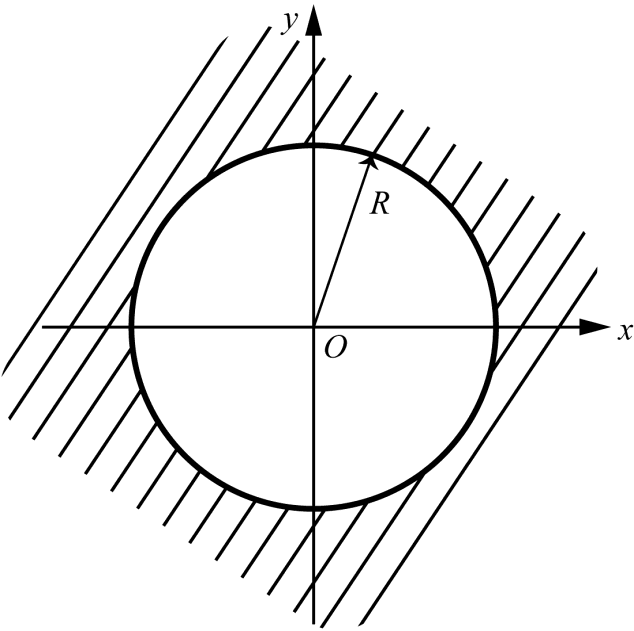
\includegraphics[keepaspectratio,alt={图4.1 幂级数的收敛圆}]{figures/04-解析函数的级数表示法/fig-p14-02b5ec75.png}}
\caption{图4.1 幂级数的收敛圆}
\end{figure}

\textbf{例 4.2} 讨论幂级数

\[
\sum_{n=0}^{\infty}z^n=1+z+z^2+\cdots+z^n+\cdots
\]

的收敛范围与和函数。

\textbf{解} 级数的部分和为

\[
s_n(z)=
\begin{cases}
\dfrac{1-z^n}{1-z}, & z\neq 1,\\[4pt]
n, & z=1.
\end{cases}
\]

该级数的收敛半径为 \(1\)，收敛圆为 \(|z|<1\)，且级数在圆周 \(|z|=1\)
上处处发散。于是

\[
\lim_{n\to\infty}s_n(z)=
\begin{cases}
\dfrac{1}{1-z}, & |z|<1,\\[4pt]
\text{发散}, & |z|\ge 1.
\end{cases}
\]

即和函数 \(s(z)=\dfrac{1}{1-z}\ (|z|<1)\)。

\subsection{4.2.3
收敛半径的求法}\label{ux6536ux655bux534aux5f84ux7684ux6c42ux6cd5}

\textbf{定理 4.6} 若 \(\displaystyle\sum_{n=0}^{\infty}a_n z^n\)
的系数满足

\[
\lim_{n\to\infty}\left|\frac{a_{n+1}}{a_n}\right|=\rho ,
\]

则

\begin{enumerate}
\def\labelenumi{\arabic{enumi}.}
\tightlist
\item
  当 \(0<\rho<+\infty\) 时，\(R=\dfrac{1}{\rho}\)；
\item
  当 \(\rho=0\) 时，\(R=+\infty\)（处处收敛）；
\item
  当 \(\rho=+\infty\) 时，\(R=0\)（仅有一个收敛点 \(z=0\)）。
\end{enumerate}

\textbf{证明要点} 考虑正项级数

\[
\sum_{n=0}^{\infty}|a_n z^n|=|a_0|+|a_1 z|+\cdots+|a_n z^n|+\cdots,
\]

其相邻项之比

\[
\lim_{n\to\infty}\left|\frac{a_{n+1}z^{n+1}}{a_n z^n}\right|=\rho|z| .
\]

\begin{itemize}
\tightlist
\item
  若 \(0<\rho<+\infty\)，由正项级数的比值判别法知，当 \(\rho|z|<1\)（即
  \(|z|<\frac{1}{\rho}\)）时 \(\sum|a_n z^n|\) 收敛，从而
  \(\sum a_n z^n\) 收敛；当 \(\rho|z|>1\)（即 \(|z|>\frac{1}{\rho}\)）时
  \(\lim\left|\frac{a_{n+1}z^{n+1}}{a_n z^n}\right|>1\)，故当 \(n\)
  充分大时 \(|a_{n+1}z^{n+1}|\ge|a_n z^n|\)，所以当 \(n\to\infty\)
  时一般项 \(a_n z^n\) 不能趋于零，级数发散。故收敛半径
  \(R=\frac{1}{\rho}\)。
\item
  若 \(\rho=0\)，则 \(\rho|z|<1\) 对任何 \(z\) 成立，故对任何 \(z\) 级数
  \(\sum|a_n z^n|\) 收敛（即处处绝对收敛），收敛半径 \(R=+\infty\)。
\item
  若 \(\rho=+\infty\)，对任意 \(z\neq 0\)，当 \(n\) 充分大时必有
  \(|a_{n+1}z^{n+1}|\ge|a_n z^n|\)，由此得 \(\sum a_n z^n\)
  发散，故收敛半径 \(R=0\)。\(\square\)
\end{itemize}

\textbf{定理 4.7} 若幂级数 \(\displaystyle\sum_{n=0}^{\infty}a_n z^n\)
的系数满足

\[
\lim_{n\to\infty}\sqrt[n]{|a_n|}=\rho ,
\]

则

\begin{enumerate}
\def\labelenumi{\arabic{enumi}.}
\tightlist
\item
  当 \(0<\rho<+\infty\) 时，\(R=\dfrac{1}{\rho}\)；
\item
  当 \(\rho=0\) 时，\(R=+\infty\)；
\item
  当 \(\rho=+\infty\) 时，\(R=0\)。
\end{enumerate}

\subsection{4.2.4
幂级数的运算及性质}\label{ux5e42ux7ea7ux6570ux7684ux8fd0ux7b97ux53caux6027ux8d28}

\textbf{性质 4.1} 若幂级数 \(\displaystyle\sum_{n=0}^{\infty}a_n z^n\)
和 \(\displaystyle\sum_{n=0}^{\infty}b_n z^n\) 的收敛半径分别为 \(R_1\)
和 \(R_2\)，则幂级数 \(\displaystyle\sum_{n=0}^{\infty}(a_n\pm b_n)z^n\)
的收敛半径不小于

\[
R=\min\{R_1,R_2\},
\]

且在 \(|z|<R\) 内有

\[
\sum_{n=0}^{\infty}a_n z^n\pm\sum_{n=0}^{\infty}b_n z^n=\sum_{n=0}^{\infty}(a_n\pm b_n)z^n .
\]

\textbf{性质 4.2} 若幂级数 \(\displaystyle\sum_{n=0}^{\infty}a_n z^n\)
和 \(\displaystyle\sum_{n=0}^{\infty}b_n z^n\) 的收敛半径分别为 \(R_1\)
和 \(R_2\)，则幂级数（Cauchy 乘积）

\[
a_0b_0+(a_0b_1+a_1b_0)z+(a_0b_2+a_1b_1+a_2b_0)z^2+\cdots+\left(\sum_{i=0}^{n}a_i b_{n-i}\right)z^n+\cdots
\]

的收敛半径不小于 \(R=\min\{R_1,R_2\}\)，且在 \(|z|<R\) 内有

\[
\left(\sum_{n=0}^{\infty}a_n z^n\right)\cdot\left(\sum_{n=0}^{\infty}b_n z^n\right)=\sum_{n=0}^{\infty}\left(\sum_{i=0}^{n}a_i b_{n-i}\right)z^n .
\]

\textbf{例 4.3} 设有幂级数 \(\displaystyle\sum_{n=0}^{\infty}z^n\) 与
\(\displaystyle\sum_{n=0}^{\infty}\frac{1}{1+a^n}z^n\)（\(0<a<1\)），求

\[
\sum_{n=0}^{\infty}\left(1-\frac{1}{1+a^n}\right)z^n=\sum_{n=0}^{\infty}\frac{a^n}{1+a^n}z^n
\]

的收敛半径。

\textbf{解} \(\displaystyle\sum_{n=0}^{\infty}z^n\) 和
\(\displaystyle\sum_{n=0}^{\infty}\frac{1}{1+a^n}z^n\) 的收敛半径都为
\(1\)，而

\[
\sum_{n=0}^{\infty}\frac{a^n}{1+a^n}z^n
\]

的收敛半径为 \(\dfrac{1}{a}\ (>1)\)。但等式

\[
\sum_{n=0}^{\infty}z^n-\sum_{n=0}^{\infty}\frac{1}{1+a^n}z^n=\sum_{n=0}^{\infty}\left(1-\frac{1}{1+a^n}\right)z^n
\]

成立的范围仍为 \(|z|<1\)。当 \(1\le|z|<\frac{1}{a}\)
时，等式左边的两个级数都不收敛，所以等式没有意义。

\subsection{4.2.5
幂级数的解析性（逐项求导与逐项积分）}\label{ux5e42ux7ea7ux6570ux7684ux89e3ux6790ux6027ux9010ux9879ux6c42ux5bfcux4e0eux9010ux9879ux79efux5206}

\textbf{定理 4.8} 设幂级数
\(\displaystyle\sum_{n=0}^{\infty}a_n(z-z_0)^n\) 的收敛半径为
\(R\)，那么

\begin{enumerate}
\def\labelenumi{\arabic{enumi}.}
\tightlist
\item
  它的和函数 \(\displaystyle f(z)=\sum_{n=0}^{\infty}a_n(z-z_0)^n\)
  在收敛圆 \(|z-z_0|<R\) 内是解析函数；
\item
  \(f(z)\) 的导数可通过对其幂级数逐项求导得到，即
\end{enumerate}

\[
f'(z)=\sum_{n=0}^{\infty}n a_n(z-z_0)^{n-1}\qquad (|z-z_0|<R);
\]

\begin{enumerate}
\def\labelenumi{\arabic{enumi}.}
\setcounter{enumi}{2}
\tightlist
\item
  \(f(z)\) 在 \(|z-z_0|<R\) 内可以逐项积分，即
\end{enumerate}

\[
\int_C f(z)\,\mathrm{d}z=\sum_{n=0}^{\infty}a_n\int_C(z-z_0)^n\,\mathrm{d}z,
\]

其中 \(C\) 为 \(|z-z_0|<R\) 内的曲线。

\textbf{例 4.4} 求出下列幂级数的和函数。

\[
(1)\ \sum_{n=1}^{\infty}(2^n-1)z^{n-1};\qquad
(2)\ \sum_{n=0}^{\infty}(n+1)z^n .
\]

\textbf{解}

\textbf{(1)}
\(\displaystyle\lim_{n\to\infty}\left|\frac{a_{n+1}}{a_n}\right|=\lim_{n\to\infty}\frac{|2^{n+1}-1|}{|2^n-1|}=2\)，故收敛半径为
\(R=\dfrac{1}{2}\)。同样 \(\sum_{n=1}^{\infty}2^n z^{n-1}\) 和
\(\sum_{n=1}^{\infty}z^{n-1}\) 的收敛半径分别为 \(R_1=\dfrac{1}{2}\) 和
\(R_2=1\)。

当 \(|z|<\dfrac{1}{2}\) 时，

\[
\sum_{n=1}^{\infty}(2^n-1)z^{n-1}=\sum_{n=1}^{\infty}2^n z^{n-1}-\sum_{n=1}^{\infty}z^{n-1}
=2\sum_{n=1}^{\infty}(2z)^{n-1}-\sum_{n=1}^{\infty}z^{n-1}
\]

\[
=2\cdot\frac{1}{1-2z}-\frac{1}{1-z}=\frac{1}{(1-2z)(1-z)} .
\]

\textbf{(2)}
\(\displaystyle\lim_{n\to\infty}\left|\frac{a_{n+1}}{a_n}\right|=\lim_{n\to\infty}\frac{n+2}{n+1}=1\)，故收敛半径为
\(R=1\)。

在 \(|z|<1\) 内取一条连接 \(0\) 和 \(z\) 的简单曲线
\(C\)，由逐项积分性质，得

\[
\int_0^z\sum_{n=0}^{\infty}(n+1)w^n\,\mathrm{d}w=\sum_{n=0}^{\infty}\int_0^z(n+1)w^n\,\mathrm{d}w=\sum_{n=0}^{\infty}z^{n+1}=\frac{z}{1-z},\qquad |z|<1 .
\]

再对两边求导，得

\[
\sum_{n=0}^{\infty}(n+1)z^n=\left(\frac{z}{1-z}\right)'=\frac{1}{(1-z)^2},\qquad |z|<1 .
\]

\subsection{常见错误与注意点}\label{ux5e38ux89c1ux9519ux8befux4e0eux6ce8ux610fux70b9-12}

\begin{itemize}
\tightlist
\item
  收敛半径只保证 \(|z|<R\) 内收敛；边界 \(|z|=R\)
  上的点可能收敛、也可能发散，必须另行判断。
\item
  定理 4.6、4.7 中 \(\rho\) 是\textbf{非负实数}，不要漏掉
  \(\rho=0\)、\(\rho=+\infty\) 两种极限情形。
\item
  幂级数做加减、乘法后，收敛半径只保证``不小于
  \(\min\{R_1,R_2\}\)''，实际半径可能更大（见例
  4.3），但在两个原级数都不收敛的区域内，用``和/差''表示的等式不成立。
\item
  逐项求导、逐项积分都在收敛圆内（开圆盘）进行，不能越过收敛圆周。
\end{itemize}

\subsection{本节小结}\label{ux672cux8282ux5c0fux7ed3-12}

\begin{itemize}
\tightlist
\item
  幂级数 \(\sum a_n(z-z_0)^n\) 的收敛域是以 \(z_0\)
  为中心的圆盘（或全平面、仅一点），边界敛散不定（§4.2.2）。
\item
  收敛半径可由比值法 \(\rho=\lim|a_{n+1}/a_n|\) 或根值法
  \(\rho=\lim\sqrt[n]{|a_n|}\) 求得，\(R=1/\rho\)（定理 4.6、4.7）。
\item
  两幂级数之和、积在 \(|z|<\min\{R_1,R_2\}\)
  上成立，且和/积级数的半径不小于该值（性质 4.1、4.2）。
\item
  收敛圆内和函数解析，可逐项求导、逐项积分（定理
  4.8），这是求幂级数和函数及泰勒展开的基础。
\end{itemize}

\section{4.3
解析函数的泰勒展开}\label{ux89e3ux6790ux51fdux6570ux7684ux6cf0ux52d2ux5c55ux5f00}

\begin{quote}
本节目标：理解解析函数在圆盘内可展开成幂级数（泰勒级数）这一基本定理，掌握展开式的唯一性、解析与有泰勒展式的等价关系、零点及其阶数判定，并牢记常用初等函数的泰勒展开式。
重点：泰勒定理（定理 4.9）及其思想；展开式唯一性；零点的阶数（\(m\)
阶零点）；\(\mathrm{e}^z\)、\(\cos z\)、\(\sin z\) 的展开。
难点：泰勒定理证明中柯西积分公式与几何级数展开、余项估计的思想；零点阶数与导数条件（性质
4.4）。
\end{quote}

对应幻灯片：第 25--32 页。

\subsection{4.3.1 泰勒定理}\label{ux6cf0ux52d2ux5b9aux7406}

\textbf{定理 4.9} 设 \(K\) 表示以 \(z_0\) 为中心、半径为 \(r\)
的一个圆，\(f(z)\) 在 \(K\) 内解析，则 \(f(z)\) 可以在 \(K\)
内展开成幂级数，即

\[
f(z)=\sum_{n=0}^{\infty}\frac{f^{(n)}(z_0)}{n!}(z-z_0)^n,\qquad z\in K .
\]

并称它为 \(f(z)\) 在 \(z_0\) 的泰勒（Taylor）展开式，上式右端的级数称为
\(f(z)\) 的泰勒级数。

\begin{figure}
\centering
\pandocbounded{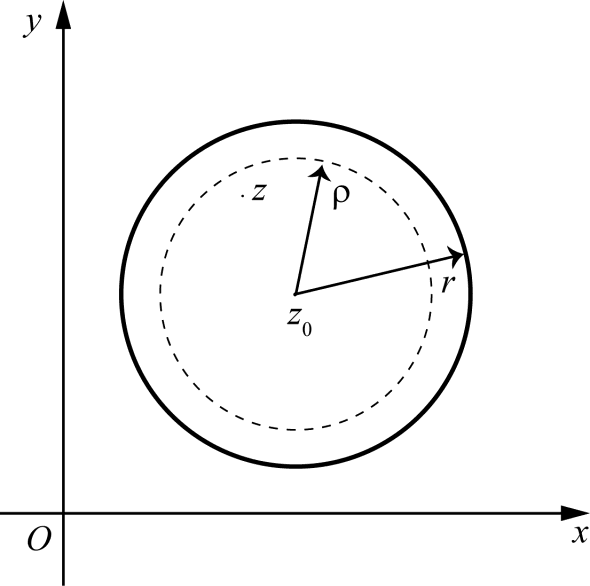
\includegraphics[keepaspectratio,alt={图4.2 泰勒展开的证明示意}]{figures/04-解析函数的级数表示法/fig-p25-54aa3acd.png}}
\caption{图4.2 泰勒展开的证明示意}
\end{figure}

\textbf{证明要点}

\begin{enumerate}
\def\labelenumi{\arabic{enumi}.}
\tightlist
\item
  任意取定 \(z\in K\)，再取正数 \(\rho\)，使 \(\rho<r\)，且
  \(|z-z_0|<\rho\)，即圆 \(|\zeta-z_0|=\rho\) 在 \(K\)
  内。根据柯西积分公式，得
\end{enumerate}

\[
f(z)=\frac{1}{2\pi\mathrm{i}}\oint_{|\zeta-z_0|=\rho}\frac{f(\zeta)}{\zeta-z}\,\mathrm{d}\zeta .
\]

\begin{enumerate}
\def\labelenumi{\arabic{enumi}.}
\setcounter{enumi}{1}
\tightlist
\item
  把 \(\dfrac{1}{\zeta-z}\) 按 \(|z-z_0|<|\zeta-z_0|\) 展开成几何级数：
\end{enumerate}

\[
\frac{1}{\zeta-z}=\frac{1}{\zeta-z_0}\cdot\frac{1}{1-\dfrac{z-z_0}{\zeta-z_0}}=\frac{1}{\zeta-z_0}\sum_{n=0}^{\infty}\left(\frac{z-z_0}{\zeta-z_0}\right)^n .
\]

代入柯西公式，并与积分号交换，得

\[
f(z)=\sum_{n=0}^{N-1}\frac{f^{(n)}(z_0)}{n!}(z-z_0)^n+R_N(z),
\]

其中

\[
R_N(z)=\frac{1}{2\pi\mathrm{i}}\oint_{|\zeta-z_0|=\rho}\left(\sum_{n=N}^{\infty}\frac{f(\zeta)}{(\zeta-z_0)^{n+1}}(z-z_0)^n\right)\mathrm{d}\zeta .
\]

\begin{enumerate}
\def\labelenumi{\arabic{enumi}.}
\setcounter{enumi}{2}
\tightlist
\item
  对给定的 \(z\)，证明 \(\lim_{N\to\infty}R_N(z)=0\)。令
\end{enumerate}

\[
q=\left|\frac{z-z_0}{\zeta-z_0}\right|=\frac{|z-z_0|}{\rho},
\]

则 \(0\le q<1\)。由于 \(f(\zeta)\) 在 \(|\zeta-z_0|=\rho\)
上连续，故有界，即存在 \(M>0\)，使 \(|f(\zeta)|\le M\)。于是

\[
|R_N(z)|\le\frac{1}{2\pi}\oint\left(\sum_{n=N}^{\infty}\frac{|f(\zeta)|}{|\zeta-z_0|}\cdot\left|\frac{z-z_0}{\zeta-z_0}\right|^n\right)|\mathrm{d}\zeta|
\le\frac{1}{2\pi}\sum_{n=N}^{\infty}\frac{M}{\rho}q^n\cdot 2\pi\rho=\frac{Mq^N}{1-q}\to 0 .
\]

\begin{enumerate}
\def\labelenumi{\arabic{enumi}.}
\setcounter{enumi}{3}
\tightlist
\item
  令 \(N\to\infty\)，得
\end{enumerate}

\[
f(z)=\sum_{n=0}^{\infty}\frac{f^{(n)}(z_0)}{n!}(z-z_0)^n .
\]

由 \(z\) 的任意性，故上式在 \(K\) 内成立。\(\square\)

\textbf{展开式的唯一性} 假设另有展开式

\[
f(z)=\sum_{n=0}^{\infty}a_n(z-z_0)^n .
\]

逐项求 \(k\) 阶导数，得

\[
f^{(k)}(z)=\sum_{n=k}^{\infty}n(n-1)\cdots(n-k+1)a_n(z-z_0)^{n-k}.
\]

令 \(z=z_0\)，即得 \(f^{(k)}(z_0)=k!\,a_k\)，所以有公式

\[
a_n=\frac{f^{(n)}(z_0)}{n!},\qquad n=0,1,2,\cdots .
\]

因此泰勒展开式是唯一的。

\subsection{4.3.2
解析性与泰勒展式、零点}\label{ux89e3ux6790ux6027ux4e0eux6cf0ux52d2ux5c55ux5f0fux96f6ux70b9}

\textbf{定理 4.10} \(f(z)\) 在 \(z_0\) 处解析的充要条件是 \(f(z)\) 在
\(z_0\) 的邻域内有泰勒展式。

设 \(f(z)\) 在 \(z_0\) 处解析且 \(f(z_0)=0\)，则称 \(z_0\) 为 \(f(z)\)
的零点。

\textbf{性质 4.3} \(z_0\) 为 \(f(z)\) 的零点的充要条件是 \(f(z)\) 在
\(z_0\) 的邻域内可以表示为

\[
f(z)=(z-z_0)^m g(z),
\]

其中 \(m\) 为某一正整数，\(g(z)\) 在 \(z_0\) 处解析且
\(g(z_0)\neq 0\)。此时称 \(z_0\) 是 \(f(z)\) 的 \(m\) 阶零点。

\textbf{性质 4.4} \(z_0\) 为 \(f(z)\) 的 \(m\) 阶零点的充要条件是

\[
f^{(n)}(z_0)=0\quad(n=0,1,\cdots,m-1),
\]

但有

\[
f^{(m)}(z_0)\neq 0 .
\]

\textbf{性质 4.5} 设 \(z_0\) 为 \(f(z)\) 的零点，且 \(f(z)\) 在 \(z_0\)
处任意阶导数都为零，即

\[
f^{(n)}(z_0)=0\quad(n=0,1,2,\cdots),
\]

则存在 \(\delta>0\)，使 \(f(z)\) 在 \(|z-z_0|<\delta\) 内恒等于零。

一个不恒为零的解析函数的零点是孤立的。

\subsection{4.3.3
常用的初等函数的泰勒展开式}\label{ux5e38ux7528ux7684ux521dux7b49ux51fdux6570ux7684ux6cf0ux52d2ux5c55ux5f00ux5f0f}

\[
\mathrm{e}^z=1+z+\cdots+\frac{z^n}{n!}+\cdots,\qquad |z|<\infty .
\]

\[
\cos z=\sum_{n=0}^{\infty}(-1)^n\frac{z^{2n}}{(2n)!}
=1-\frac{z^2}{2!}+\frac{z^4}{4!}-+\cdots+(-1)^n\frac{z^{2n}}{(2n)!}+\cdots,\qquad |z|<\infty .
\]

\[
\sin z=\sum_{n=0}^{\infty}(-1)^n\frac{z^{2n+1}}{(2n+1)!}
=z-\frac{z^3}{3!}+\frac{z^5}{5!}-+\cdots+(-1)^n\frac{z^{2n+1}}{(2n+1)!}+\cdots,\qquad |z|<\infty .
\]

\subsection{4.3.4 例题}\label{ux4f8bux9898-2}

\textbf{例 4.5} 把函数 \(\dfrac{1}{(1+z)^2}\) 展开成 \(z-1\) 的幂级数。

\textbf{解}

\[
\frac{1}{(1+z)^2}=\frac{1}{4}\cdot\frac{1}{\left(1+\dfrac{z-1}{2}\right)^2}=\frac{1}{4}\cdot\frac{1}{(1+\zeta)^2}\qquad\left(\zeta=\frac{z-1}{2}\right).
\]

先写出

\[
\frac{1}{1+\zeta}=1-\zeta+\zeta^2-\cdots+(-1)^n\zeta^n+\cdots,\qquad|\zeta|<1 .
\]

两端求导得

\[
\frac{1}{(1+\zeta)^2}=1-2\zeta+3\zeta^2-4\zeta^3+\cdots+(-1)^{n-1}n\zeta^{n-1}+\cdots,\qquad|\zeta|<1 .
\]

代入 \(\zeta=\dfrac{z-1}{2}\)，得

\[
\frac{1}{(1+z)^2}=\frac{1}{4}\left(1-2\cdot\frac{z-1}{2}+3\left(\frac{z-1}{2}\right)^2-\cdots+(-1)^{n-1}n\left(\frac{z-1}{2}\right)^{n-1}+\cdots\right)
\]

\[
=\sum_{n=1}^{\infty}(-1)^{n-1}\frac{n}{2^{n+1}}(z-1)^{n-1},\qquad |z-1|<2 .
\]

\subsection{常见错误与注意点}\label{ux5e38ux89c1ux9519ux8befux4e0eux6ce8ux610fux70b9-13}

\begin{itemize}
\tightlist
\item
  泰勒级数是``圆盘内''的展开；在边界圆周上不能保证展开式收敛或与函数相等。
\item
  展开式唯一：无论用什么方法得到的幂级数，其系数必为
  \(f^{(n)}(z_0)/n!\)。
\item
  \(\cos z\) 展开式中只含偶次幂、\(\sin z\)
  只含奇次幂，且符号交替；展开式中不得混入错误幂次（如把 \(\cos z\)
  写成含 \(z^5\) 项即错）。
\item
  零点阶数判定：\(z_0\) 为 \(m\) 阶零点
  \(\iff f(z_0)=\cdots=f^{(m-1)}(z_0)=0\) 且
  \(f^{(m)}(z_0)\neq 0\)；注意``直到前一阶导数为零、阶导数不为零''。
\item
  不恒为零的解析函数的零点是孤立的，这一点在后续洛朗展开与孤立奇点中很重要。
\end{itemize}

\subsection{本节小结}\label{ux672cux8282ux5c0fux7ed3-13}

\begin{itemize}
\tightlist
\item
  圆盘内解析 \(\Rightarrow\) 可展开为收敛的泰勒级数（定理
  4.9），且展开式唯一。
\item
  证明的核心是柯西积分公式 + 几何级数展开 + 余项趋于零（\(q<1\)）。
\item
  泰勒级数存在 \(\iff\) 函数在该点解析（定理 4.10）。
\item
  零点的阶数可由 \(f(z)=(z-z_0)^m g(z)\) 或导数条件（性质
  4.3、4.4）判定。
\item
  常用的 \(\mathrm{e}^z\)、\(\cos z\)、\(\sin z\)
  展开式必须熟练记忆并会用于``换元''展开（见例 4.5）。
\end{itemize}

\section{4.4
解析函数的洛朗展开}\label{ux89e3ux6790ux51fdux6570ux7684ux6d1bux6717ux5c55ux5f00}

\begin{quote}
本节目标：理解洛朗级数（双向级数）及其收敛域------圆环，掌握洛朗定理（在圆环内解析可展开、且唯一），并会用部分分式法在给定圆环内求函数的洛朗展开。
重点：正幂级数与负幂级数的收敛域合成圆环；洛朗定理；给定圆环内的洛朗展开（例
4.6、4.7）。
难点：负幂级数的收敛域（\(|z-z_0|>r\)）理解；在不同圆环内展开式不同；洛朗展开唯一性指``在给定圆环内''唯一。
\end{quote}

对应幻灯片：第 33--42 页。

\subsection{\texorpdfstring{4.4.1 洛朗级数（\(z-z_0\)
的双向级数）}{4.4.1 洛朗级数（z-z\_0 的双向级数）}}\label{ux6d1bux6717ux7ea7ux6570z-z_0-ux7684ux53ccux5411ux7ea7ux6570}

考虑级数

\[
\sum_{n=-\infty}^{\infty}a_n(z-z_0)^n=\cdots+a_{-n}(z-z_0)^{-n}+\cdots+a_{-1}(z-z_0)^{-1}+a_0+a_1(z-z_0)+\cdots+a_n(z-z_0)^n+\cdots,
\]

其中 \(z_0\) 和 \(a_n\ (n=0,\pm1,\pm2,\cdots)\) 为常数，\(z\) 为变量。

把它分成两部分：

\begin{itemize}
\tightlist
\item
  \(z-z_0\) 的\textbf{正幂级数}：
\end{itemize}

\[
\sum_{n=0}^{\infty}a_n(z-z_0)^n=a_0+a_1(z-z_0)+a_2(z-z_0)^2+\cdots+a_n(z-z_0)^n+\cdots;
\]

\begin{itemize}
\tightlist
\item
  \(z-z_0\) 的\textbf{负幂级数}：
\end{itemize}

\[
\sum_{n=1}^{\infty}a_{-n}(z-z_0)^{-n}=a_{-1}(z-z_0)^{-1}+a_{-2}(z-z_0)^{-2}+\cdots+a_{-n}(z-z_0)^{-n}+\cdots .
\]

\subsection{4.4.2 收敛域：圆环}\label{ux6536ux655bux57dfux5706ux73af}

如果在 \(z=z_1\) 处，\(z-z_0\) 的正幂级数和 \(z-z_0\)
的负幂级数都收敛，就称 \(z_1\) 为级数
\(\displaystyle\sum_{n=-\infty}^{\infty}a_n(z-z_0)^n\)
的一个收敛点；不是收敛点的点就称为该级数的发散点。

\(z-z_0\) 的正幂级数，它的收敛范围是圆盘 \(|z-z_0|<R\)，且 \(|z-z_0|>R\)
时级数发散。

\(z-z_0\) 的负幂级数

\[
\sum_{n=1}^{\infty}a_{-n}(z-z_0)^{-n}=\sum_{n=1}^{\infty}a_{-n}\zeta^n\qquad\left(\zeta=\frac{1}{z-z_0}\right),
\]

它的收敛半径为 \(\rho\)，则当 \(|\zeta|<\rho\) 时收敛、\(|\zeta|>\rho\)
时发散。记 \(r=\dfrac{1}{\rho}\)，于是负幂级数当 \(|z-z_0|>r\)
时收敛，而 \(|z-z_0|<r\) 时发散。

因此 \(\displaystyle\sum_{n=-\infty}^{\infty}a_n(z-z_0)^n\)
的收敛集合取决于 \(r\) 和 \(R\)。

\begin{enumerate}
\def\labelenumi{\arabic{enumi}.}
\tightlist
\item
  若
  \(r>R\)，此时正幂级数和负幂级数没有公共的收敛范围，故级数在复平面上处处发散。
\item
  若 \(r<R\)，此时正幂级数和负幂级数的公共收敛范围是圆环
  \(r<|z-z_0|<R\)，所以级数在这个圆环内收敛，而在其外部发散。在其边界
  \(|z-z_0|=r\) 和 \(|z-z_0|=R\) 上级数可能有收敛点，也可能有发散点。
\item
  若 \(r=R\)，此时级数在 \(|z-z_0|=R\) 以外的点处处发散，而在
  \(|z-z_0|=R\) 上的点无法直接断定其收敛性，要根据具体情况而定。
\end{enumerate}

\begin{figure}
\centering
\pandocbounded{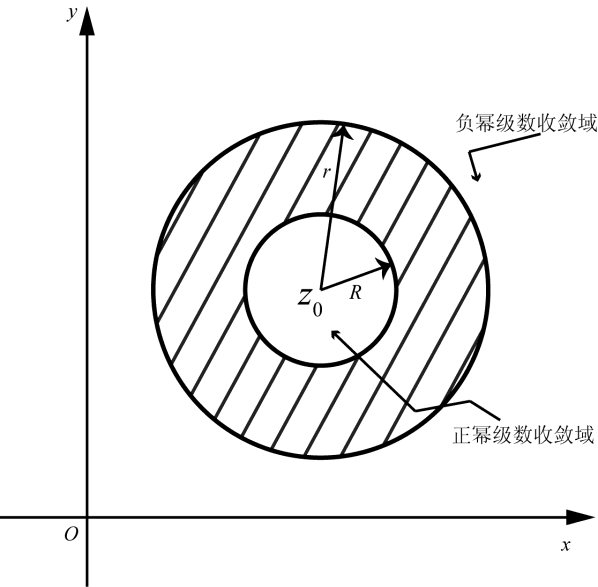
\includegraphics[keepaspectratio,alt={图4.3 洛朗级数：r\textgreater R 时正、负幂级数无公共收敛域}]{figures/04-解析函数的级数表示法/fig-p35-7df0dd55.png}}
\caption{图4.3 洛朗级数：\(r>R\) 时正、负幂级数无公共收敛域}
\end{figure}

\begin{figure}
\centering
\pandocbounded{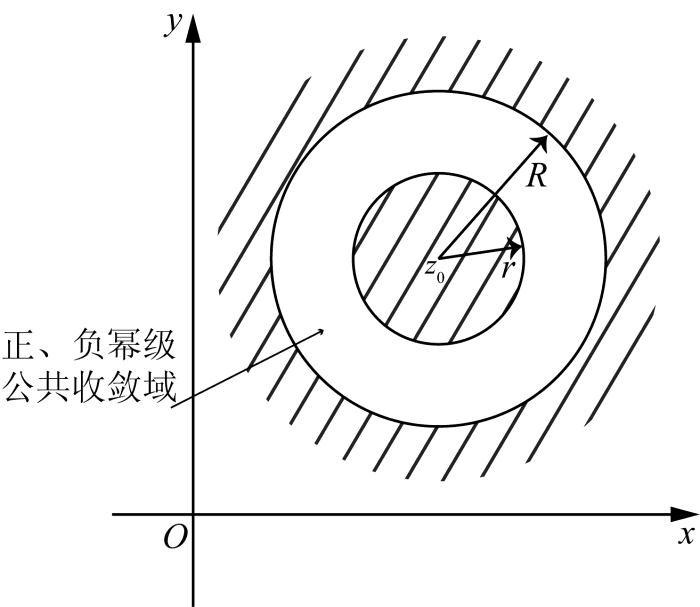
\includegraphics[keepaspectratio,alt={图4.4 洛朗级数：r\textless R 时收敛圆环}]{figures/04-解析函数的级数表示法/fig-p35-e4a70a30.png}}
\caption{图4.4 洛朗级数：\(r<R\) 时收敛圆环}
\end{figure}

\textbf{定理 4.11} 级数
\(\displaystyle\sum_{n=-\infty}^{\infty}a_n(z-z_0)^n\)
在其收敛圆环内的和函数是解析的，而且可以逐项积分和逐项求导数。

\textbf{例 4.6} 讨论级数

\[
\sum_{n=1}^{\infty}\frac{a^n}{z^n}+\sum_{n=0}^{\infty}\frac{z^n}{b^n}
\]

的收敛集，并求和函数，其中 \(a\) 与 \(b\) 为复常数。

\textbf{解} 分别讨论负幂级数和正幂级数。

\textbf{负幂级数}
\(\displaystyle\sum_{n=1}^{\infty}\left(\frac{a}{z}\right)^n\)：当
\(\left|\dfrac{a}{z}\right|<1\)，即 \(|z|>|a|\) 时收敛，且和函数为

\[
\frac{a}{z-a}.
\]

\textbf{正幂级数}
\(\displaystyle\sum_{n=0}^{\infty}\left(\frac{z}{b}\right)^n\)：当
\(\left|\dfrac{z}{b}\right|<1\)，即 \(|z|<|b|\) 时收敛，且和函数为

\[
\frac{b}{b-z}.
\]

（注：正幂级数收敛条件是 \(|z|<|b|\)，这样才能与负幂级数合成圆环
\(|a|<|z|<|b|\)。）

\begin{itemize}
\tightlist
\item
  当 \(|a|<|b|\) 时，原级数收敛且收敛圆环为 \(|a|<|z|<|b|\)，和函数为
\end{itemize}

\[
\frac{a}{z-a}+\frac{b}{b-z}=\frac{(a-b)z}{(a-z)(b-z)} .
\]

\begin{itemize}
\tightlist
\item
  当 \(|a|>|b|\)
  时，负幂级数和正幂级数的收敛域没有公共点，故原级数发散。
\end{itemize}

在圆环 \(|a|<|z|<|b|\) 内解析的函数 \(\dfrac{(a-b)z}{(a-z)(b-z)}\)
可以展开为级数：

\[
\frac{(a-b)z}{(a-z)(b-z)}=\sum_{n=1}^{\infty}\frac{a^n}{z^n}+\sum_{n=0}^{\infty}\frac{z^n}{b^n}.
\]

\subsection{4.4.3 洛朗定理}\label{ux6d1bux6717ux5b9aux7406}

\textbf{定理 4.12} 设 \(f(z)\) 在圆环 \(r<|z-z_0|<R\) 内解析，那么

\[
f(z)=\sum_{n=-\infty}^{\infty}a_n(z-z_0)^n,\qquad r<|z-z_0|<R,
\]

其中

\[
a_n=\frac{1}{2\pi\mathrm{i}}\oint_C\frac{f(\zeta)}{(\zeta-z_0)^{n+1}}\,\mathrm{d}\zeta,\qquad n=0,\pm1,\pm2,\cdots,
\]

这里 \(C\) 为圆环 \(r<|z-z_0|<R\) 内任何一条绕 \(z_0\)
的正向简单闭曲线，且 \(f(z)\) 的表达式是唯一的。

\(f(z)=\displaystyle\sum_{n=-\infty}^{\infty}a_n(z-z_0)^n\ (r<|z-z_0|<R)\)
称为函数 \(f(z)\) 在以 \(z_0\) 为中心的圆环 \(r<|z-z_0|<R\)
内的\textbf{洛朗（Laurent）展开式}。它的右端称为在此圆环内的洛朗级数。

\begin{figure}
\centering
\pandocbounded{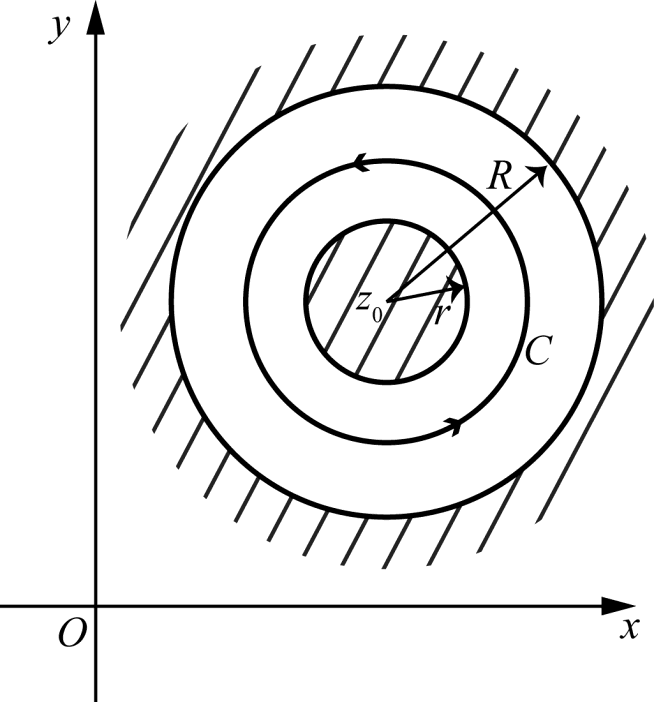
\includegraphics[keepaspectratio,alt={图4.5 洛朗展开的圆环与积分曲线 C}]{figures/04-解析函数的级数表示法/fig-p38-74ee3c5a.png}}
\caption{图4.5 洛朗展开的圆环与积分曲线 \(C\)}
\end{figure}

\textbf{洛朗展开式的唯一性}
所谓洛朗展开式的唯一性，是指函数在某一个给定的圆环的洛朗展开式是唯一的。

\subsection{4.4.4
求洛朗展开的例题}\label{ux6c42ux6d1bux6717ux5c55ux5f00ux7684ux4f8bux9898}

\textbf{例 4.7} 求函数 \(\displaystyle f(z)=\frac{1}{(z-1)(z-2)}\)
在下列圆环内的洛朗级数。

\[
(1)\ 0<|z|<1;\qquad
(2)\ 1<|z|<2;\qquad
(3)\ 2<|z|<+\infty;
\]

\[
(4)\ 0<|z-1|<1;\qquad
(5)\ 1<|z-1|<+\infty .
\]

\textbf{解} 将函数表示成部分分式，有

\[
f(z)=\frac{1}{1-z}-\frac{1}{2-z}.
\]

\textbf{(1)} 在 \(0<|z|<1\) 内，由于 \(|z|<1\)，因此
\(\left|\dfrac{z}{2}\right|<1\)，故

\[
\frac{1}{1-z}=1+z+z^2+\cdots+z^n+\cdots,
\]

\[
\frac{1}{2-z}=\frac{1}{2}\cdot\frac{1}{1-z/2}=\frac{1}{2}\left(1+\frac{z}{2}+\frac{z^2}{4}+\cdots+\frac{z^n}{2^n}+\cdots\right).
\]

于是

\[
f(z)=\left(1+z+z^2+\cdots\right)-\frac{1}{2}\left(1+\frac{z}{2}+\frac{z^2}{4}+\cdots\right)=\sum_{n=0}^{\infty}\left(1-\frac{1}{2^{n+1}}\right)z^n
=\frac{1}{2}+\frac{3}{4}z+\frac{7}{8}z^2+\cdots .
\]

\textbf{(2)} 在 \(1<|z|<2\)
内，\(\left|\dfrac{1}{z}\right|<1\)、\(\left|\dfrac{z}{2}\right|<1\)，故

\[
f(z)=\frac{1}{1-z}-\frac{1}{2-z}=-\frac{1}{z}\cdot\frac{1}{1-1/z}-\frac{1}{2}\cdot\frac{1}{1-z/2}
\]

\[
=-\frac{1}{z}\left(1+\frac{1}{z}+\frac{1}{z^2}+\cdots\right)-\frac{1}{2}\left(1+\frac{z}{2}+\frac{z^2}{4}+\cdots\right)
=-\sum_{n=1}^{\infty}\frac{1}{z^n}-\sum_{n=0}^{\infty}\frac{z^n}{2^{n+1}} .
\]

\textbf{(3)} 在 \(2<|z|<+\infty\)
内，\(\left|\dfrac{1}{z}\right|<1\)、\(\left|\dfrac{2}{z}\right|<1\)，故

\[
f(z)=\frac{1}{1-z}-\frac{1}{2-z}=-\frac{1}{z}\cdot\frac{1}{1-1/z}+\frac{1}{z}\cdot\frac{1}{1-2/z}
\]

\[
=-\frac{1}{z}\left(1+\frac{1}{z}+\frac{1}{z^2}+\cdots\right)+\frac{1}{z}\left(1+\frac{2}{z}+\frac{4}{z^2}+\cdots\right)
=\frac{1}{z^2}+\frac{3}{z^3}+\frac{7}{z^4}+\cdots .
\]

\textbf{(4)} 在 \(0<|z-1|<1\) 内，有

\[
f(z)=\frac{1}{z-2}-\frac{1}{z-1}=-\frac{1}{1-(z-1)}-\frac{1}{z-1}
=-\sum_{n=0}^{\infty}(z-1)^n-\frac{1}{z-1} .
\]

即

\[
f(z)=-\frac{1}{z-1}-1-(z-1)-(z-1)^2-\cdots-(z-1)^n-\cdots .
\]

\textbf{(5)} 在 \(1<|z-1|<+\infty\)
内，\(\left|\dfrac{1}{z-1}\right|<1\)，故

\[
f(z)=\frac{1}{(z-1)-1}-\frac{1}{z-1}=\frac{1}{z-1}\cdot\frac{1}{1-1/(z-1)}-\frac{1}{z-1},
\]

\[
=\frac{1}{z-1}+\frac{1}{(z-1)^2}+\cdots+\frac{1}{(z-1)^n}+\cdots-\frac{1}{z-1}
=\frac{1}{(1-z)^2}+\frac{1}{(z-1)^3}+\cdots+\frac{1}{(z-1)^n}+\cdots .
\]

更简洁地，

\[
f(z)=\sum_{n=2}^{\infty}\frac{1}{(z-1)^n}\qquad(1<|z-1|<\infty).
\]

\subsection{常见错误与注意点}\label{ux5e38ux89c1ux9519ux8befux4e0eux6ce8ux610fux70b9-14}

\begin{itemize}
\tightlist
\item
  洛朗展开的\textbf{收敛域是圆环} \(r<|z-z_0|<R\)，其中 \(r\)
  由负幂级数确定（\(|z-z_0|>r\)），\(R\)
  由正幂级数确定（\(|z-z_0|<R\)）。不要把负幂级数的收敛域也写成圆盘。
\item
  同一个函数在不同的圆环内，洛朗展开式不同；唯一性是指``在给定的某一个圆环内''唯一。
\item
  求洛朗展开一般先做部分分式，再在\textbf{指定的}圆环内选择合适的形式展开：缺项要补
  \(1\)，且必须保证展开所用公比绝对值小于 \(1\)（例 4.7 中分别以
  \(\frac{z}{2}\)、\(\frac{1}{z}\)、\(\frac{2}{z}\)、\(\frac{1}{z-1}\)
  等为公比）。
\item
  例 4.6 中正幂级数 \(\sum(z/b)^n\) 的收敛条件是
  \(|z|<|b|\)（幻灯片上``\(|z|>|b|\)''为笔误），它与负幂级数的
  \(|z|>|a|\) 合成圆环 \(|a|<|z|<|b|\)。
\end{itemize}

\subsection{本节小结}\label{ux672cux8282ux5c0fux7ed3-14}

\begin{itemize}
\tightlist
\item
  洛朗级数是``正幂级数 + 负幂级数''的双向级数，其收敛域一般是圆环
  \(r<|z-z_0|<R\)（还可能是空集、圆盘、圆内去心等退化情形）。
\item
  圆环内解析函数必有洛朗展开，且唯一（定理
  4.12）；系数由围道积分给出，实际求法常用部分分式 + 几何级数。
\item
  圆环内和函数解析，可逐项求导、逐项积分（定理 4.11）。
\item
  洛朗展开是研究孤立奇点分类（§4.5）的直接工具：负幂项的多少决定奇点类型。
\end{itemize}

\section{4.5 孤立奇点}\label{ux5b64ux7acbux5947ux70b9}

\begin{quote}
本节目标：掌握孤立奇点的定义，并能依据洛朗展开式中负幂项的有无与多少，把孤立奇点分成可去奇点、极点、本性奇点三类；掌握极点与零点的关系、本性奇点的刻画（定理
4.14），并会讨论无穷远点的奇点性质。
重点：三类孤立奇点的洛朗级数判别；\(m\) 阶极点与 \(1/f(z)\) 的 \(m\)
阶零点的关系；无穷远点的奇点分类。
难点：负幂项``多少个''与奇点类型的对应；无穷远点作变换 \(z=1/t\)
后的奇点归属；例 4.8 中零极点阶数与可去奇点的判断。
\end{quote}

对应幻灯片：第 43--50 页。

\subsection{4.5.1
孤立奇点的定义与分类}\label{ux5b64ux7acbux5947ux70b9ux7684ux5b9aux4e49ux4e0eux5206ux7c7b}

\textbf{定义 4.4} 若 \(z=z_0\) 为函数 \(f(z)\)
的一个奇点，且存在一个去心邻域 \(0<|z-z_0|<\delta\)，\(f(z)\)
在其中处处解析，则称 \(z_0\) 为 \(f(z)\) 的\textbf{孤立奇点}。

设 \(z_0\) 为 \(f(z)\) 的一个孤立奇点，因为在 \(0<|z-z_0|<\delta\)
中解析，\(f(z)\) 可展开成 \(z-z_0\) 的洛朗级数，即

\[
f(z)=\sum_{n=0}^{\infty}a_n(z-z_0)^n+\sum_{n=1}^{\infty}a_{-n}(z-z_0)^{-n}.
\]

根据洛朗级数中负幂项的情况，把孤立奇点分成三类：

\begin{enumerate}
\def\labelenumi{\arabic{enumi}.}
\tightlist
\item
  级数中不出现负幂项，此时称点 \(z_0\) 为 \(f(z)\) 的\textbf{可去奇点}；
\item
  级数中只含有有限个负幂项，则点 \(z_0\) 称为 \(f(z)\) 的\textbf{极点}；
\item
  级数中含有无穷多个负幂项，点 \(z_0\) 称为 \(f(z)\)
  的\textbf{本性奇点}。
\end{enumerate}

\subsection{4.5.2 可去奇点}\label{ux53efux53bbux5947ux70b9}

\(f(z)\) 在 \(0<|z-z_0|<\delta\) 内的洛朗级数实际为一个幂级数

\[
a_0+a_1(z-z_0)+a_2(z-z_0)^2+\cdots+a_n(z-z_0)^n+\cdots .
\]

这个幂级数在圆盘 \(|z-z_0|<\delta\) 内是收敛的，其和函数为

\[
F(z)=
\begin{cases}
a_0, & z=z_0,\\[4pt]
f(z), & 0<|z-z_0|<\delta .
\end{cases}
\]

\(F(z)\) 在 \(|z-z_0|<\delta\) 内解析。所以不论 \(f(z)\) 原来在 \(z_0\)
是否有定义，我们用 \(F(z)\) 来代替 \(f(z)\)，或令
\(f(z_0)=a_0\)，这样就把奇点除去了。由于这个原因，所以 \(z_0\)
称为可去奇点。

\subsection{4.5.3 极点}\label{ux6781ux70b9}

设 \(z=z_0\) 为函数 \(f(z)\) 的极点。若 \(f(z)\) 在 \(0<|z-z_0|<\delta\)
内洛朗展开式为

\[
f(z)=\frac{a_{-m}}{(z-z_0)^m}+\cdots+\frac{a_{-1}}{z-z_0}+\sum_{n=0}^{\infty}a_n(z-z_0)^n,\qquad(m\ge 1,\ a_{-m}\neq 0),
\]

则称 \(z_0\) 为 \(f(z)\) 的 \(m\) 阶极点。

此时可写成

\[
f(z)=\frac{1}{(z-z_0)^m}\varphi(z),
\]

其中

\[
\varphi(z)=a_{-m}+a_{-m+1}(z-z_0)+a_{-m+2}(z-z_0)^2+\cdots+a_{-1}(z-z_0)^{m-1}+\sum_{n=0}^{\infty}a_n(z-z_0)^{n+m},
\]

\(\varphi(z)\) 在 \(|z-z_0|<\delta\) 内解析且
\(\varphi(z_0)=a_{-m}\neq 0\)。反之，若有在 \(|z-z_0|<\delta\)
内解析且在 \(z_0\) 处函数值不为零的函数
\(\varphi\)，使得上面这种洛朗展开式成立，则容易看出 \(z_0\) 为 \(f(z)\)
的 \(m\) 阶极点。

\textbf{定理 4.13} 如果 \(z_0\) 是 \(f(z)\) 的 \(m\) 阶极点，那么
\(z_0\) 就是 \(\dfrac{1}{f(z)}\) 的 \(m\) 阶零点。反过来也成立。

\subsection{4.5.4 本性奇点}\label{ux672cux6027ux5947ux70b9}

\textbf{定理 4.14（Weierstrass 定理）} 如果 \(z_0\) 为 \(f(z)\)
的本性奇点，那么对于任意给定的复数 \(A\)，总可以找到一个趋于 \(z_0\)
的数列 \(\{z_n\}\)，使得

\[
\lim_{n\to\infty}f(z_n)=A .
\]

\(f(z)\) 的孤立奇点 \(z_0\) 的邻域中，按可去奇点、极点、本性奇点的顺次有

\[
(1)\ \lim_{z\to z_0}f(z)=\text{有限数};
\]

\[
(2)\ \lim_{z\to z_0}f(z)=\infty;
\]

\[
(3)\ \lim_{z\to z_0}f(z)\ \text{不存在}.
\]

\subsection{4.5.5
函数在无穷远点的性质}\label{ux51fdux6570ux5728ux65e0ux7a77ux8fdcux70b9ux7684ux6027ux8d28}

如果函数 \(f(z)\) 是在无穷远点 \(z=\infty\) 的去心邻域 \(R<|z|<\infty\)
内解析，那么称点 \(\infty\) 为 \(f(z)\) 的孤立奇点。

作变换 \(\displaystyle z=\frac{1}{t}\)，记
\(\displaystyle g(t)=f\left(\frac{1}{t}\right)\)，则 \(g(t)\) 在
\(0<|t|<\frac{1}{R}\) 中解析，即 \(t=0\) 是 \(g(t)\) 的孤立奇点。

如果 \(t=0\) 是 \(g(t)\) 的可去奇点、\(m\)
阶极点或是本性奇点，那么就称点 \(z=\infty\) 是 \(f(z)\)
的可去奇点、\(m\) 阶极点或本性奇点。

因为 \(g(t)\) 在原点的邻域内有洛朗展式：

\[
g(t)=\sum_{n=-\infty}^{\infty}a_n t^n,\qquad 0<|t|<\frac{1}{R},
\]

所以 \(f(z)\) 在 \(R<|z|<\infty\) 中有下面的洛朗展式

\[
f(z)=\sum_{n=-\infty}^{\infty}b_n z^n,\qquad R<|z|<\infty,
\]

其中

\[
b_n=a_{-n}\ (n=0,\pm1,\pm2,\cdots),\qquad
b_n=\frac{1}{2\pi\mathrm{i}}\oint_C\frac{f(\zeta)}{\zeta^{n+1}}\,\mathrm{d}\zeta,\qquad n=0,\pm1,\pm2,\cdots,
\]

其中 \(C\) 为圆环域 \(R<|z|<\infty\) 内绕原点的任何一条正向简单闭曲线。

在级数
\(f(z)=\displaystyle\sum_{n=-\infty}^{\infty}b_n z^n\ (R<|z|<\infty)\)
中：

\begin{enumerate}
\def\labelenumi{\arabic{enumi}.}
\tightlist
\item
  不含正幂项 \(\iff\) \(\infty\) 为可去奇点 \(\iff\)
  \(\lim_{z\to\infty}f(z)\) 存在；
\item
  含有有限多个正幂项，且 \(z^m\) 为最高正幂 \(\iff\) \(\infty\) 为 \(m\)
  阶极点 \(\iff\) \(\lim_{z\to\infty}f(z)=\infty\)；
\item
  含有无穷多正幂项 \(\iff\) \(\infty\) 为本性奇点 \(\iff\)
  \(\lim_{z\to\infty}f(z)\) 不存在。
\end{enumerate}

\subsection{4.5.6 例题}\label{ux4f8bux9898-3}

\textbf{例 4.8} 函数
\(\displaystyle f(z)=\frac{(\mathrm{e}^z-1)(z-2)^4}{(\sin\pi z)^4}\)
在扩充的复平面上有无奇点？是什么类型？若是极点，求出其阶。

\textbf{解} 函数有奇点 \(0,\pm1,\pm2,\cdots\) 和
\(\infty\)。这是因为函数在这些点无定义，所以是奇点。

\textbf{(1)} \(z=0\) 是 \(\sin\pi z\) 的一阶零点，从而是
\((\sin\pi z)^4\) 的四阶零点；但它又是分子 \(\mathrm{e}^z-1\)
的一阶零点（因为 \(\mathrm{e}^z-1\) 在 \(z=0\) 处为零且导数
\(\mathrm{e}^0=1\neq 0\)），故 \(z=0\) 是函数的三阶极点（\(4-1=3\)）。

\textbf{(2)} 同 (1)，\(\pm1,-2,\pm3,\pm4,\cdots\) 是函数的四阶极点（对
\(k\neq 0,2\)，分子 \((\mathrm{e}^k-1)(k-2)^4\neq 0\)，而
\((\sin\pi k)^4\) 为四阶零点）。

\textbf{(3)} \(z=2\) 是可去奇点。

\[
\lim_{z\to2}f(z)=\lim_{z\to2}(\mathrm{e}^z-1)\cdot\lim_{z\to2}\left(\frac{z-2}{\sin\pi z}\right)^4
=(\mathrm{e}^2-1)\cdot\frac{1}{\pi^4}.
\]

因为
\(\lim_{z\to2}\dfrac{z-2}{\sin\pi z}=\dfrac{1}{\pi\cos 2\pi}=\dfrac{1}{\pi}\)，所以极限为有限数，故
\(z=2\) 为可去奇点。

\textbf{(4)} 考察 \(\infty\)：令 \(z=1/t\)，则

\[
f\left(\frac{1}{t}\right)=\frac{(\mathrm{e}^{1/t}-1)(1-2t)^4}{t^4\left(\sin\dfrac{\pi}{t}\right)^4}.
\]

所以 \(t=0\) 及 \(t_n=\dfrac{1}{n}\ (n=1,2,\cdots)\) 均为上式的奇点。当
\(n\to\infty\) 时，\(t_n\to0\)，所以 \(t=0\) 不是 \(f(1/t)\)
的孤立奇点，也就是说 \(z=\infty\) 不是 \(f(z)\) 的孤立奇点。

\subsection{常见错误与注意点}\label{ux5e38ux89c1ux9519ux8befux4e0eux6ce8ux610fux70b9-15}

\begin{itemize}
\tightlist
\item
  判断奇点类型必须\textbf{先看洛朗展开式中负幂项}：无负幂项（可去）、有限个负幂项（极点）、无穷多个负幂项（本性奇点）。
\item
  ``\(m\) 阶零点''与``\(m\) 阶极点''互为倒数的关系（定理
  4.13）非常常用：分子零点阶数与分母零点阶数相减即得极点阶数（例 4.8）。
\item
  若分子、分母在同一零点处都有零点，要相抵（如 \(z=2\)：分子 \((z-2)^4\)
  四阶零点与分母 \((\sin\pi z)^4\) 四阶零点抵消，成为可去奇点）。
\item
  无穷远点必须先作变换 \(z=1/t\) 化为原点 \(t=0\) 研究；并根据 \(g(t)\)
  的洛朗级数（即 \(f(z)\) 的级数中\textbf{正幂项}）来判别。
\item
  记法：对无穷远点，正幂项（\(z^n,\ n>0\)）的多少对应 \(\infty\)
  的奇点类型，与有限孤立奇点看负幂项正好对偶。
\end{itemize}

\subsection{本节小结}\label{ux672cux8282ux5c0fux7ed3-15}

\begin{itemize}
\tightlist
\item
  孤立奇点由去心邻域内解析定义（定义 4.4），其洛朗级数负幂项决定类型。
\item
  可去奇点：无负幂项，可通过补充定义值 \(f(z_0)=a_0\) 使函数解析。
\item
  \(m\) 阶极点：负幂项最高为 \((z-z_0)^{-m}\)，等价于
  \(f(z)=\dfrac{\varphi(z)}{(z-z_0)^m}\)，\(\varphi(z_0)\neq 0\)；且
  \(z_0\) 是 \(1/f(z)\) 的 \(m\) 阶零点（定理 4.13）。
\item
  本性奇点：无穷多个负幂项；由定理 4.14，其极限不存在（且值在 \(z_0\)
  附近任意接近任何复数 \(A\)）。
\item
  无穷远点的奇点性质通过 \(z=1/t\) 转化为原点奇点研究；正幂项决定
  \(\infty\) 的类型（§4.5.5）。
\end{itemize}

\newpage

\chaptercover{5}{留数理论及其应用}
%% 由 build/emit_tex.py 生成（生成物，勿手改）；定制请放 user_style.tex / user_meta.yaml
\chapter{第 5 章 ·
留数理论及其应用}\label{ux7b2c-5-ux7ae0-ux7559ux6570ux7406ux8bbaux53caux5176ux5e94ux7528}

\section{5.1 留数}\label{ux7559ux6570}

\begin{quote}
\textbf{本节目标}：理解留数的定义与几何意义，掌握留数定理及其证明，熟练运用极点的留数计算公式以及``商函数''留数公式，并了解无穷远点留数的概念与``全体奇点留数之和为零''的定理。
\textbf{重点}：留数的定义、留数定理、极点留数的计算（\(m\) 阶极点公式与
\(P(z)/Q(z)\) 公式）。
\textbf{难点}：无穷远点的留数概念，以及用洛朗展开求 \(a_{-1}\) 的技巧。
\end{quote}

\subsection{5.1.1 留数的定义}\label{ux7559ux6570ux7684ux5b9aux4e49}

设 \(z_0\) 是 \(f(z)\)
的\textbf{孤立奇点}。那么，对于解析圆环(去心邻域)内包含 \(z_0\)
的正向简单闭曲线 \(C\)，积分

\[
\oint_C f(\zeta)\,\mathrm d\zeta
\]

只与 \(f(z)\) 和 \(z_0\) 有关，而与 \(C\)
的选择无关；但该积分值不一定为零。

\(f(z)\) 在 \(z_0\) 的去心邻域内可展开成\textbf{洛朗级数}：

\[
f(z)=\sum_{n=-\infty}^{\infty}a_n\,(z-z_0)^{n},
\]

其中

\[
a_n=\frac{1}{2\pi\mathrm i}\oint_C\frac{f(\zeta)}{(\zeta-z_0)^{n+1}}\,\mathrm d\zeta,\qquad n=0,\pm1,\pm2,\ldots
\]

特别地，当 \(n=-1\) 时，

\[
a_{-1}=\frac{1}{2\pi\mathrm i}\oint_C f(\zeta)\,\mathrm d\zeta .
\]

\textbf{定义 5.1（留数）} 把 \(f(z)\) 在 \(z_0\) 处的洛朗级数中
\((z-z_0)^{-1}\) 项的系数 \(a_{-1}\) 称为 \(f(z)\) 在孤立奇点 \(z_0\)
处的\textbf{留数}，记作

\[
\operatorname{Res}\bigl[f(z),z_0\bigr]=a_{-1},
\]

即

\[
\operatorname{Res}\bigl[f(z),z_0\bigr]
=\frac{1}{2\pi\mathrm i}\oint_C f(z)\,\mathrm dz .
\]

\textbf{例 5.1} 求下列积分的值，其中 \(C\) 为包含 \(z=0\)
的简单正向闭曲线：

\[
(1)\ \oint_C z^{-3}\cos z\,\mathrm dz;\qquad
(2)\ \oint_C \mathrm e^{\frac{1}{z^{2}}}\,\mathrm dz .
\]

\textbf{解} （1）令 \(f(z)=z^{-3}\cos z\)，则 \(z=0\) 为 \(f(z)\)
的孤立奇点。由

\[
\cos z=1-\frac{z^{2}}{2!}+\frac{z^{4}}{4!}-\frac{z^{6}}{6!}+\cdots,\qquad |z|<\infty,
\]

得

\[
f(z)=\frac{1}{z^{3}}-\frac{1}{2}\cdot\frac{1}{z}+\frac{z}{4!}-\frac{z^{3}}{6!}+\cdots,\qquad 0<|z|<\infty .
\]

所以 \(\operatorname{Res}\bigl[f(z),0\bigr]=-\dfrac12\)，从而

\[
\oint_C z^{-3}\cos z\,\mathrm dz=-\pi\mathrm i .
\]

（2）令 \(f(z)=\mathrm e^{1/z^{2}}\)，则 \(z=0\) 为 \(f(z)\)
的孤立奇点。由

\[
\mathrm e^{\zeta}=1+\frac{\zeta}{1!}+\frac{\zeta^{2}}{2!}+\cdots+\frac{\zeta^{n}}{n!}+\cdots,\qquad |\zeta|<\infty,
\]

以 \(\zeta=\dfrac{1}{z^{2}}\) 代入，得

\[
f(z)=1+\frac{1}{1!}\cdot\frac{1}{z^{2}}+\frac{1}{2!}\cdot\frac{1}{z^{4}}+\cdots+\frac{1}{n!}\cdot\frac{1}{z^{2n}}+\cdots,\qquad 0<|z|<\infty .
\]

此展开式中不含 \((z-0)^{-1}\) 项，所以
\(\operatorname{Res}\bigl[f(z),0\bigr]=0\)，于是

\[
\oint_C \mathrm e^{1/z^{2}}\,\mathrm dz=0 .
\]

\subsection{5.1.2 留数定理}\label{ux7559ux6570ux5b9aux7406}

\textbf{定理 5.1（留数定理）} 设函数 \(f(z)\) 在区域 \(D\)
内除有有限个孤立奇点 \(z_1,z_2,\ldots,z_n\) 外处处解析，\(C\) 是 \(D\)
内包围这些奇点的一条正向简单闭曲线，那么

\[
\oint_C f(z)\,\mathrm dz
=2\pi\mathrm i\sum_{k=1}^{n}\operatorname{Res}\bigl[f(z),z_k\bigr].
\]

\begin{figure}
\centering
\pandocbounded{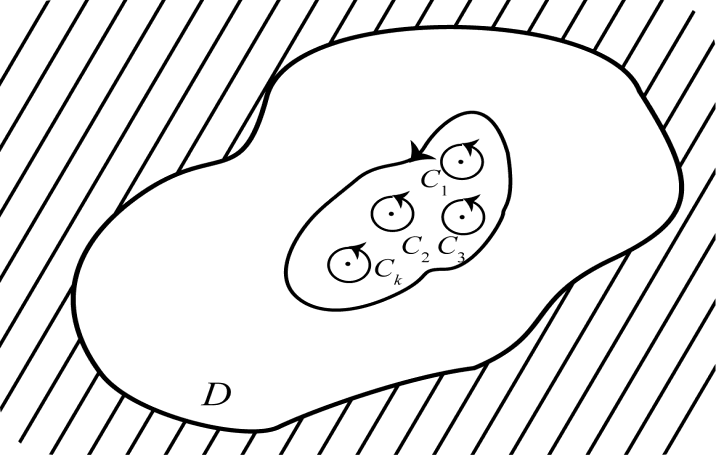
\includegraphics[keepaspectratio,alt={图5.1 留数定理：包围奇点的复合闭路}]{figures/05-留数理论及其应用/fig-p06-5116eeae.png}}
\caption{图5.1 留数定理：包围奇点的复合闭路}
\end{figure}

\textbf{证明要点} 以 \(z_k\) 为圆心，作完全含在 \(C\)
内且互不相交的正向小圆

\[
C_k:\ |z-z_k|=\delta_k,\qquad (k=1,2,\ldots,n).
\]

由复合闭路上的柯西积分定理，有

\[
\oint_C f(z)\,\mathrm dz
=\oint_{C_1} f(z)\,\mathrm dz
+\oint_{C_2} f(z)\,\mathrm dz
+\cdots+\oint_{C_n} f(z)\,\mathrm dz .
\]

但由留数的定义，

\[
\oint_{C_k} f(z)\,\mathrm dz=2\pi\mathrm i\operatorname{Res}\bigl[f(z),z_k\bigr],\qquad k=1,2,\ldots,n,
\]

故

\[
\oint_C f(z)\,\mathrm dz
=2\pi\mathrm i\sum_{k=1}^{n}\operatorname{Res}\bigl[f(z),z_k\bigr].
\]

\subsection{5.1.3
留数的计算方法}\label{ux7559ux6570ux7684ux8ba1ux7b97ux65b9ux6cd5}

\subsubsection{\texorpdfstring{(1) \(m\)
阶极点的留数公式}{(1) m 阶极点的留数公式}}\label{m-ux9636ux6781ux70b9ux7684ux7559ux6570ux516cux5f0f}

\textbf{公式 5.1} 如果 \(z_0\) 为 \(f(z)\) 的 \(m\) 阶极点，那么

\[
\operatorname{Res}\bigl[f(z),z_0\bigr]
=\frac{1}{(m-1)!}\lim_{z\to z_0}\frac{\mathrm d^{\,m-1}}{\mathrm d z^{\,m-1}}
\Bigl\{(z-z_0)^{m}\,f(z)\Bigr\}.
\]

\textbf{证明要点} 因为 \(z_0\) 是 \(f(z)\) 的 \(m\) 阶极点，故在 \(z_0\)
的邻域中有

\[
f(z)=\frac{g(z)}{(z-z_0)^{m}},
\]

其中 \(g(z)\) 在 \(z_0\) 处解析，且 \(g(z_0)\neq0\)。于是

\[
f(z)=\frac{1}{(z-z_0)^{m}}\sum_{n=0}^{\infty}\frac{g^{(n)}(z_0)}{n!}(z-z_0)^{n}
=\sum_{n=0}^{\infty}\frac{g^{(n)}(z_0)}{n!}(z-z_0)^{n-m}.
\]

其中 \((z-z_0)^{-1}\) 项的系数为（令 \(n-m=-1\)，即 \(n=m-1\)）

\[
\frac{g^{(m-1)}(z_0)}{(m-1)!}.
\]

又 \(g(z)=(z-z_0)^{m}f(z)\)，因而得到

\[
\frac{g^{(m-1)}(z_0)}{(m-1)!}
=\frac{1}{(m-1)!}\lim_{z\to z_0}\frac{\mathrm d^{\,m-1}}{\mathrm d z^{\,m-1}}
\Bigl\{(z-z_0)^{m}\,f(z)\Bigr\}.
\]

\subsubsection{(2)
一阶极点的留数公式}\label{ux4e00ux9636ux6781ux70b9ux7684ux7559ux6570ux516cux5f0f}

若 \(z_0\) 是 \(f(z)\) 的一阶极点，则由上式取 \(m=1\)，得

\[
\operatorname{Res}\bigl[f(z),z_0\bigr]
=\lim_{z\to z_0}(z-z_0)\,f(z).
\]

\subsubsection{(3)
商函数的留数公式}\label{ux5546ux51fdux6570ux7684ux7559ux6570ux516cux5f0f}

\textbf{公式 5.2} 设 \(f(z)=\dfrac{P(z)}{Q(z)}\)，\(P(z),Q(z)\) 在
\(z_0\) 处都是解析的。如果

\[
P(z_0)\neq0,\qquad Q(z_0)=0,\qquad Q'(z_0)\neq0,
\]

那么 \(z_0\) 是 \(f(z)\) 的一阶极点，因此有

\[
\operatorname{Res}\bigl[f(z),z_0\bigr]=\frac{P(z_0)}{Q'(z_0)}.
\]

\textbf{证明要点} 因 \(Q(z_0)=0\) 且 \(Q'(z_0)\neq0\)，所以 \(z_0\) 为
\(Q(z)\) 的一级零点，从而

\[
\frac{1}{Q(z)}=\frac{1}{z-z_0}\,\varphi(z),
\]

其中 \(\varphi(z)\) 在 \(z_0\) 处解析且 \(\varphi(z_0)\neq0\)。于是

\[
f(z)=\frac{1}{z-z_0}\,\varphi(z)\,P(z),
\]

且 \(\varphi(z_0)P(z_0)\neq0\)，故 \(z_0\) 为 \(f(z)\) 的一阶极点。于是

\[
\begin{aligned}
\operatorname{Res}\bigl[f(z),z_0\bigr]
&=\lim_{z\to z_0}(z-z_0)f(z)
=\lim_{z\to z_0}(z-z_0)\frac{P(z)}{Q(z)}\\
&=\lim_{z\to z_0}\frac{P(z)}{\dfrac{Q(z)-Q(z_0)}{z-z_0}}
=\frac{P(z_0)}{Q'(z_0)}.
\end{aligned}
\]

\textbf{例 5.2} 求 \(f(z)=\dfrac{5z-2}{z(z-1)^{2}}\) 分别在 \(z=0\) 和
\(z=1\) 的留数。

\textbf{解} \(z=0\) 是 \(f(z)\) 的一阶极点，故

\[
\operatorname{Res}\bigl[f(z),0\bigr]
=\lim_{z\to0}z\,f(z)
=\lim_{z\to0}\frac{5z-2}{(z-1)^{2}}=-2 .
\]

\(z=1\) 是 \(f(z)\) 的二阶极点，得

\[
\begin{aligned}
\operatorname{Res}\bigl[f(z),1\bigr]
&=\lim_{z\to1}\frac{\mathrm d}{\mathrm dz}\Bigl\{(z-1)^{2}f(z)\Bigr\}
=\lim_{z\to1}\frac{\mathrm d}{\mathrm dz}\left\{\frac{5z-2}{z}\right\}\\
&=\lim_{z\to1}\frac{5z-(5z-2)}{z^{2}}
=\lim_{z\to1}\frac{2}{z^{2}}=2 .
\end{aligned}
\]

\textbf{例 5.3} 计算 \(f(z)=\dfrac{\mathrm e^{z}}{\sin z}\) 在 \(z=0\)
处的留数。

\textbf{解} 取 \(P(z)=\mathrm e^{z}\)，\(Q(z)=\sin z\)，于是

\[
P(0)=1,\qquad Q(0)=0,\qquad Q'(0)=1,
\]

故

\[
\operatorname{Res}\bigl[f(z),0\bigr]=\frac{P(0)}{Q'(0)}=1 .
\]

\textbf{例 5.4} 计算 \(f(z)=\dfrac{z-\sin z}{z^{6}}\) 在 \(z=0\)
处的留数。

\textbf{解} 因为

\[
\begin{aligned}
\frac{z-\sin z}{z^{6}}
&=\frac{1}{z^{6}}\left[z-\left(z-\frac{1}{3!}z^{3}+\frac{1}{5!}z^{5}-\cdots\right)\right]\\
&=\frac{1}{3!}\cdot\frac{1}{z^{3}}-\frac{1}{5!}\cdot\frac{1}{z}+\cdots,
\end{aligned}
\]

所以

\[
\operatorname{Res}\left[\frac{z-\sin z}{z^{6}}\,,\,z_0\right]=a_{-1}=-\frac{1}{5!}.
\]

\textbf{例 5.5} 计算积分

\[
\oint_C \frac{z}{(z^{2}-1)^{2}(z^{2}+1)}\,\mathrm dz,
\]

这里 \(C:\ |z-1|=\sqrt3\)，取正向。

\textbf{解} 令

\[
f(z)=\frac{z}{(z^{2}-1)^{2}(z^{2}+1)},
\]

则 \(z_1=\mathrm i\)、\(z_2=-\mathrm i\) 为 \(f(z)\)
的两个一阶极点，\(z_3=1\)、\(z_4=-1\) 为 \(f(z)\) 的两个二阶极点。其中
\(z_1,z_2,z_3\) 位于 \(C\) 的内部（\(z_4=-1\) 在 \(C\) 外）。

由留数定理，

\[
\oint_C f(z)\,\mathrm dz=2\pi\mathrm i\sum_{k=1}^{3}\operatorname{Res}\bigl[f(z),z_k\bigr].
\]

计算得

\[
\operatorname{Res}\bigl[f(z),\mathrm i\bigr]
=\lim_{z\to\mathrm i}(z-\mathrm i)f(z)
=\lim_{z\to\mathrm i}\frac{z}{(z^{2}-1)^{2}(z+\mathrm i)}
=\frac{1}{8},
\]

\[
\operatorname{Res}\bigl[f(z),-\mathrm i\bigr]=\frac{1}{8},
\]

\[
\begin{aligned}
\operatorname{Res}\bigl[f(z),1\bigr]
&=\lim_{z\to1}\frac{\mathrm d}{\mathrm dz}\Bigl\{(z-1)^{2}f(z)\Bigr\}
=\lim_{z\to1}\frac{\mathrm d}{\mathrm dz}\left\{\frac{z}{(z+1)^{2}(z^{2}+1)}\right\}\\
&=\lim_{z\to1}\frac{-3z^{3}-z^{2}-z+1}{(z+1)^{3}(z^{2}+1)^{2}}
=-\frac{1}{8}.
\end{aligned}
\]

于是

\[
\oint_C f(z)\,\mathrm dz
=2\pi\mathrm i\left(\frac{1}{8}+\frac{1}{8}-\frac{1}{8}\right)
=\frac{\pi\mathrm i}{4}.
\]

\begin{quote}
\textbf{注} 这里 \(z_3=1\) 是二阶极点，其留数等于函数
\(\dfrac{z}{(z+1)^{2}(z^{2}+1)}\) 在 \(z=1\) 处的导数，结果为
\(-\dfrac18\)（容易误算为 \(+\dfrac18\)）。
\end{quote}

\subsection{5.1.4
在无穷远点的留数}\label{ux5728ux65e0ux7a77ux8fdcux70b9ux7684ux7559ux6570}

设函数 \(f(z)\) 在圆环域 \(R<|z|<\infty\) 内解析，\(C\)
为这圆环域内绕原点的任何一条简单闭曲线，那么称 \(f(z)\) 沿 \(C\)
的\textbf{负向}积分值

\[
\frac{1}{2\pi\mathrm i}\oint_{C^{-}}f(z)\,\mathrm dz
\]

为 \(f(z)\) 在点 \(\infty\) 的\textbf{留数}，记作

\[
\operatorname{Res}\bigl[f(z),\infty\bigr]
=\frac{1}{2\pi\mathrm i}\oint_{C^{-}}f(z)\,\mathrm dz
=\frac{1}{2\pi\mathrm i}\oint_{C}f(z)\,\mathrm dz
=-b_{-1},
\]

其中 \(b_{-1}\) 是 \(f(z)\) 在 \(\infty\) 点的去心邻域 \(R<|z|<\infty\)
内的洛朗展开式中 \(z^{-1}\) 的系数。

\textbf{一句话结论}：\(f(z)\) 在点 \(\infty\) 的留数，等于它在
\(\infty\) 点的去心邻域 \(R<|z|<\infty\) 内的洛朗展开式中 \(z^{-1}\)
的系数的相反数。

\textbf{定理 5.2} 如果函数 \(f(z)\)
在扩充的复平面内只有有限个孤立奇点，那么 \(f(z)\) 在所有奇点（包括
\(\infty\) 点）的留数之和为零：

\[
\operatorname{Res}\bigl[f(z),\infty\bigr]+\sum_{k=1}^{n}\operatorname{Res}\bigl[f(z),z_k\bigr]=0 .
\]

\textbf{证明要点} 取 \(r\) 充分大，使 \(f(z)\) 的有限个孤立奇点
\(z_k\ (k=1,2,\ldots,n)\) 都在 \(|z|<r\) 中。由留数定理，得

\[
\oint_{|z|<r}f(z)\,\mathrm dz
=2\pi\mathrm i\sum_{k=1}^{n}\operatorname{Res}\bigl[f(z),z_k\bigr],
\]

其中积分取圆周的正向。由无穷远点留数的定义，

\[
\operatorname{Res}\bigl[f(z),\infty\bigr]=-\oint_{|z|<r}f(z)\,\mathrm dz,
\]

于是就有

\[
\operatorname{Res}\bigl[f(z),\infty\bigr]+\sum_{k=1}^{n}\operatorname{Res}\bigl[f(z),z_k\bigr]=0 .
\]

\textbf{例 5.6} 判定 \(z=\infty\) 是函数 \(f(z)=\dfrac{2z}{3+z^{2}}\)
的什么奇点？并求 \(f(z)\) 在 \(\infty\) 点的留数。

\textbf{解} 因为

\[
\lim_{z\to\infty}f(z)=0,
\]

所以 \(\infty\) 点是\textbf{可去奇点}。\(f(z)\) 在复平面内仅有
\(\sqrt3\,\mathrm i\) 和 \(-\sqrt3\,\mathrm i\) 两个一阶极点：

\[
\operatorname{Res}\bigl[f(z),\sqrt3\mathrm i\bigr]
=\lim_{z\to\sqrt3\mathrm i}\frac{2z}{z+\sqrt3\mathrm i}=1,
\]

\[
\operatorname{Res}\bigl[f(z),-\sqrt3\mathrm i\bigr]
=\lim_{z\to-\sqrt3\mathrm i}\frac{2z}{z-\sqrt3\mathrm i}=1.
\]

由定理 5.2，

\[
\begin{aligned}
\operatorname{Res}\bigl[f(z),\infty\bigr]
&=-\operatorname{Res}\bigl[f(z),\sqrt3\mathrm i\bigr]-\operatorname{Res}\bigl[f(z),-\sqrt3\mathrm i\bigr]\\
&=-1-1=-2 .
\end{aligned}
\]

\subsection{常见错误与注意点}\label{ux5e38ux89c1ux9519ux8befux4e0eux6ce8ux610fux70b9-12}

\begin{enumerate}
\def\labelenumi{\arabic{enumi}.}
\tightlist
\item
  \textbf{留数只对孤立奇点有意义}。若 \(z_0\)
  不是孤立奇点（如本性奇点的聚点、非孤立奇点），不能直接写
  \(\operatorname{Res}[f,z_0]\)。
\item
  \textbf{\(m\) 阶极点公式别忘了 \((m-1)!\)}。很多同学把分母写成
  \(m!\)，导致结果差一个因子 \(m\)。
\item
  \textbf{二阶极点的留数需取导数}。例如例 5.5 中
  \(\operatorname{Res}[f,1]\) 是 \(\dfrac{z}{(z+1)^2(z^2+1)}\) 在
  \(z=1\) 的导数，而不是该点的函数值；要先约去
  \((z-1)^2\)，再求导、再取极限。
\item
  \textbf{无穷远点留数的符号}。\(\operatorname{Res}[f,\infty]\)
  等于洛朗展开中 \(z^{-1}\) 系数 \(b_{-1}\)
  的\textbf{相反数}，符号极易漏掉。
\item
  \textbf{用洛朗展开求 \(a_{-1}\) 时，要抓住``被积函数展开式里
  \((z-z_0)^{-1}\) 项的系数''}，不要与其它项混淆；例 5.1(2) 中
  \(e^{1/z^2}\) 的展开不含 \(z^{-1}\) 项，故留数为 \(0\)。
\end{enumerate}

\subsection{本节小结}\label{ux672cux8282ux5c0fux7ed3-12}

\begin{itemize}
\tightlist
\item
  留数 \(a_{-1}\) 刻画了 \(f\) 在孤立奇点邻域内``\(\frac{1}{z-z_0}\)
  分量''的大小，且
  \(\operatorname{Res}[f,z_0]=\frac{1}{2\pi\mathrm i}\oint_C f\,\mathrm dz\)。
\item
  \textbf{留数定理}
  把闭曲线上的复积分化为有限个孤立奇点留数之和：\(\oint_C f\,\mathrm dz=2\pi\mathrm i\sum_k\operatorname{Res}[f,z_k]\)。
\item
  计算留数的常用工具：

  \begin{itemize}
  \tightlist
  \item
    洛朗展开（求 \(a_{-1}\)）；
  \item
    \(m\) 阶极点公式
    \(\dfrac{1}{(m-1)!}\lim\dfrac{\mathrm d^{m-1}}{\mathrm dz^{m-1}}\{(z-z_0)^mf(z)\}\)；
  \item
    一阶极点 \(\lim(z-z_0)f(z)\)；
  \item
    商函数 \(\dfrac{P(z)}{Q(z)}\) 的一阶极点
    \(\dfrac{P(z_0)}{Q'(z_0)}\)。
  \end{itemize}
\item
  无穷远点留数满足 \(\operatorname{Res}[f,\infty]=-b_{-1}\)，且当 \(f\)
  在扩充平面上只有有限个孤立奇点时，全体奇点（含 \(\infty\)）留数之和为
  \(0\)。
\end{itemize}

\section{5.2
留数在积分计算上的应用}\label{ux7559ux6570ux5728ux79efux5206ux8ba1ux7b97ux4e0aux7684ux5e94ux7528}

\begin{quote}
\textbf{本节目标}：掌握用留数计算三类常见实定积分（有理函数无穷积分、含
\(e^{\alpha \mathrm i x}\) 的积分、三角有理式
\(R(\sin\theta,\cos\theta)\)
的周期积分）的方法，并能用留数计算若干特殊定积分（\(\sin x/x\)、Fresnel
积分）。
\textbf{重点}：把实积分化为闭路复积分并利用留数定理求值；合理选取积分周线与验证``圆弧上积分趋于零''。
\textbf{难点}：积分周线的构造（半圆、带小圆弧的``避点周线''、扇形周线），以及
Jordan 不等式用来估计圆弧积分。
\end{quote}

\subsection{\texorpdfstring{5.2.1 形如
\(\displaystyle\int_{-\infty}^{+\infty}R(x)\,\mathrm dx\)
的积分}{5.2.1 形如 \textbackslash displaystyle\textbackslash int\_\{-\textbackslash infty\}\^{}\{+\textbackslash infty\}R(x)\textbackslash,\textbackslash mathrm dx 的积分}}\label{ux5f62ux5982-displaystyleint_-inftyinftyrxmathrm-dx-ux7684ux79efux5206}

设

\[
R(x)=\frac{P(x)}{Q(x)}
\]

为有理函数，其中

\[
P(x)=x^{m}+a_1x^{m-1}+\cdots+a_m,\qquad
Q(x)=x^{n}+b_1x^{n-1}+\cdots+b_n,
\]

\(P(x),Q(x)\) 为两个既约实多项式，\(Q(x)\) 没有实零点，且 \(n-m\ge2\)。

把 \(x\) 换成复变量 \(z\)，得到复函数

\[
R(z)=\frac{P(z)}{Q(z)},
\]

则除 \(Q(z)\) 的有限个零点外，\(R(z)\) 处处解析。

\begin{figure}
\centering
\pandocbounded{\includegraphics[keepaspectratio,alt={图5.2 半圆周线：{[}-r,r{]} 与上半圆弧 C\_r}]{figures/05-留数理论及其应用/fig-p18-fe74c3b0.png}}
\caption{图5.2 半圆周线：\([-r,r]\) 与上半圆弧 \(C_r\)}
\end{figure}

取积分周线 \(C_r\) 为 \(x\) 轴上 \([-r,r]\) 与上半平面圆弧 \(C_r\)
所围成的闭路。由留数定理，得

\[
\int_{-r}^{r}R(x)\,\mathrm dx+\int_{C_r}R(z)\,\mathrm dz
=2\pi\mathrm i\sum_{k=1}^{s}\operatorname{Res}\bigl[R(z),z_k\bigr],
\]

其中 \(z_k\ (k=1,2,\ldots,s)\) 是 \(R(z)\) 在上半平面内的孤立奇点。当
\(r\) 充分大时，右端的值与 \(r\) 无关。

为求 \(r\to\infty\) 时的极限，先估计圆弧上的积分。由

\[
|R(z)|=\frac{1}{|z|^{n-m}}\cdot\frac{\bigl|1+a_1z^{-1}+\cdots+a_mz^{-m}\bigr|}{\bigl|1+b_1z^{-1}+\cdots+b_nz^{-n}\bigr|}
\le\frac{1}{|z|^{n-m}}\cdot\frac{1+|a_1z^{-1}|+\cdots+|a_mz^{-m}|}{1-|b_1z^{-1}|-\cdots-|b_nz^{-n}|},
\]

故存在常数 \(M\)，当 \(|z|\) 充分大时，有

\[
|R(z)|\le\frac{M}{|z|^{n-m}}\le\frac{M}{|z|^{2}}.
\]

令 \(z=r\mathrm e^{\mathrm i\theta}\)，于是

\[
\Bigl|\int_{C_r}R(z)\,\mathrm dz\Bigr|
\le\int_{0}^{\pi}\frac{M}{r^{2}}\,r\,\mathrm d\theta
=\frac{\pi M}{r}\to0\quad(r\to\infty).
\]

令 \(r\to\infty\)，得

\[
\boxed{\displaystyle\int_{-\infty}^{+\infty}R(x)\,\mathrm dx
=2\pi\mathrm i\sum_{k=1}^{s}\operatorname{Res}\bigl[R(z),z_k\bigr]},
\]

其中 \(z_k\) 为 \(R(z)\) 在上半平面内的孤立奇点。

\textbf{例 5.7} 计算积分

\[
\int_{-\infty}^{+\infty}\frac{x^{2}-x+2}{x^{4}+10x^{2}+9}\,\mathrm dx .
\]

\textbf{解} 记

\[
R(z)=\frac{z^{2}-z+2}{z^{4}+10z^{2}+9},
\]

则 \(R(z)\) 在上半平面内有 \(2\) 个一阶极点 \(z_1=\mathrm i\) 和
\(z_2=3\mathrm i\)。

\[
\operatorname{Res}\bigl[R(z),\mathrm i\bigr]=\frac{-1-\mathrm i}{16},\qquad
\operatorname{Res}\bigl[R(z),3\mathrm i\bigr]=\frac{3-7\mathrm i}{48}.
\]

于是

\[
\begin{aligned}
\int_{-\infty}^{+\infty}\frac{x^{2}-x+2}{x^{4}+10x^{2}+9}\,\mathrm dx
&=2\pi\mathrm i\left(\frac{-1-\mathrm i}{16}+\frac{3-7\mathrm i}{48}\right)\\
&=2\pi\mathrm i\cdot\frac{-5\mathrm i}{24}
=\frac{5}{12}\pi .
\end{aligned}
\]

\textbf{例 5.8} 计算积分

\[
\int_{0}^{+\infty}\frac{x^{2}}{1+x^{4}}\,\mathrm dx .
\]

\textbf{解} \(R(x)=\dfrac{x^{2}}{1+x^{4}}\) 为偶函数，故

\[
\int_{0}^{+\infty}\frac{x^{2}}{1+x^{4}}\,\mathrm dx
=\frac12\int_{-\infty}^{+\infty}\frac{x^{2}}{1+x^{4}}\,\mathrm dx .
\]

\(R(z)=\dfrac{z^{2}}{1+z^{4}}\)
的分母高于分子两次，在实轴上无奇点，在上半平面上有两个一阶极点

\[
z_1=\frac{\sqrt2}{2}(1+\mathrm i),\qquad
z_2=\frac{\sqrt2}{2}(-1+\mathrm i),
\]

其留数为

\[
\operatorname{Res}\bigl[R(z),z_1\bigr]=\frac{1-\mathrm i}{4\sqrt2},\qquad
\operatorname{Res}\bigl[R(z),z_2\bigr]=-\frac{1+\mathrm i}{4\sqrt2}.
\]

（幻灯片把这两个留数分别写成 \(\dfrac{1+\mathrm i}{4\sqrt2\,\mathrm i}\)
与 \(\dfrac{1-\mathrm i}{4\sqrt2\,\mathrm i}\)，二者等价。）于是

\[
\begin{aligned}
\int_{-\infty}^{+\infty}\frac{x^{2}}{1+x^{4}}\,\mathrm dx
&=2\pi\mathrm i\left(-\frac{2\mathrm i}{4\sqrt2}\right)
=\frac{\pi}{\sqrt2}=\frac{\sqrt2}{2}\pi,\\
\int_{0}^{+\infty}\frac{x^{2}}{1+x^{4}}\,\mathrm dx
&=\frac12\cdot\frac{\sqrt2}{2}\pi=\frac{\sqrt2}{4}\pi .
\end{aligned}
\]

\subsection{\texorpdfstring{5.2.2 形如
\(\displaystyle\int_{-\infty}^{+\infty}R(x)\mathrm e^{\alpha\mathrm i x}\,\mathrm dx\ (\alpha>0)\)
的积分}{5.2.2 形如 \textbackslash displaystyle\textbackslash int\_\{-\textbackslash infty\}\^{}\{+\textbackslash infty\}R(x)\textbackslash mathrm e\^{}\{\textbackslash alpha\textbackslash mathrm i x\}\textbackslash,\textbackslash mathrm dx\textbackslash{} (\textbackslash alpha\textgreater0) 的积分}}\label{ux5f62ux5982-displaystyleint_-inftyinftyrxmathrm-ealphamathrm-i-xmathrm-dx-alpha0-ux7684ux79efux5206}

设 \(R(x)\) 是实轴上连续的有理函数，而分母的次数 \(n\)
至少要比分子的次数 \(m\) 高一次（\(n-m\ge1\)），且 \(R\)
在实轴上无奇点。取积分曲线 \(C_r\)（\([-r,r]\) 与上半圆弧 \(C_r\)），当
\(r\) 充分大时，使 \(z_k\ (k=1,2,\ldots,s)\) 全落在曲线 \(C_r\) 与
\([-r,r]\) 所围成的区域内。

\begin{figure}
\centering
\pandocbounded{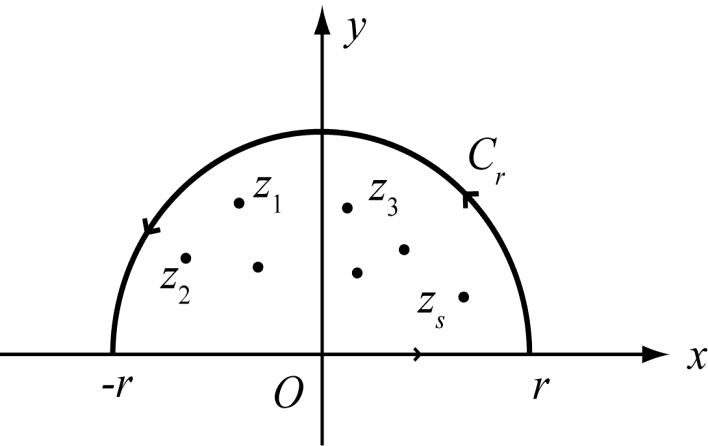
\includegraphics[keepaspectratio,alt={图5.3 上半圆周线及其中的极点}]{figures/05-留数理论及其应用/fig-p22-fe74c3b0.png}}
\caption{图5.3 上半圆周线及其中的极点}
\end{figure}

由留数定理，

\[
\int_{-r}^{r}R(x)\mathrm e^{\alpha\mathrm i x}\,\mathrm dx
+\int_{C_r}R(z)\mathrm e^{\alpha\mathrm i z}\,\mathrm dz
=2\pi\mathrm i\sum_{k=1}^{s}\operatorname{Res}\bigl[R(z)\mathrm e^{\alpha\mathrm i z},z_k\bigr].
\]

又 \(n-m\ge1\)，故当 \(|z|\) 充分大时，有

\[
|R(z)|\le\frac{M}{|z|}.
\]

因此

\[
\begin{aligned}
\Bigl|\int_{C_r}R(z)\mathrm e^{\alpha\mathrm i z}\,\mathrm dz\Bigr|
&=\Bigl|\int_{0}^{\pi}R(r\mathrm e^{\mathrm i\theta})\mathrm e^{\alpha\mathrm i r\mathrm e^{\mathrm i\theta}}\cdot \mathrm i r\mathrm e^{\mathrm i\theta}\,\mathrm d\theta\Bigr|\\
&\le M\int_{0}^{\pi}\mathrm e^{-\alpha r\sin\theta}\,\mathrm d\theta
=2M\int_{0}^{\pi/2}\mathrm e^{-\alpha r\sin\theta}\,\mathrm d\theta .
\end{aligned}
\]

当 \(0\le\theta\le\dfrac{\pi}{2}\)
时，\(\sin\theta\ge\dfrac{2\theta}{\pi}\)（Jordan 不等式），所以有

\[
\Bigl|\int_{C_r}R(z)\mathrm e^{\alpha\mathrm i z}\,\mathrm dz\Bigr|
\le2M\int_{0}^{\pi/2}\mathrm e^{-\alpha r\frac{2\theta}{\pi}}\,\mathrm d\theta
=\frac{M\pi}{\alpha r}\,\bigl(1-\mathrm e^{-\alpha r}\bigr)\to0\quad(r\to\infty).
\]

\begin{quote}
\textbf{注} 幻灯片此处写为
\(\dfrac{M\pi}{2r}(1-\mathrm e^{-\alpha r})\)，漏掉了分母中的
\(\alpha\)。按 Jordan 不等式严格计算应为
\(\dfrac{M\pi}{\alpha r}(1-\mathrm e^{-\alpha r})\)。
\end{quote}

当 \(r\to\infty\)
时，\(\displaystyle\int_{C_r}R(z)\mathrm e^{\alpha\mathrm i z}\,\mathrm dz\to0\)，得

\[
\boxed{\displaystyle\int_{-\infty}^{+\infty}R(x)\mathrm e^{\alpha\mathrm i x}\,\mathrm dx
=2\pi\mathrm i\sum_{k=1}^{s}\operatorname{Res}\bigl[R(z)\mathrm e^{\alpha\mathrm i z},z_k\bigr]} .
\]

分开实、虚部，即

\[
\int_{-\infty}^{+\infty}R(x)\cos\alpha x\,\mathrm dx
+\mathrm i\int_{-\infty}^{+\infty}R(x)\sin\alpha x\,\mathrm dx
=2\pi\mathrm i\sum_{k=1}^{s}\operatorname{Res}\bigl[R(z)\mathrm e^{\alpha\mathrm i z},z_k\bigr].
\]

\textbf{例 5.9} 求积分

\[
\int_{-\infty}^{+\infty}\frac{\cos x}{x^{2}+4x+5}\,\mathrm dx .
\]

\textbf{解} 设

\[
R(z)=\frac{1}{z^{2}+4z+5},
\]

则 \(R(z)\) 的分母高于分子二次，实轴上无奇点，上半平面只有一个一阶极点
\(z=-2+\mathrm i\)。于是

\[
\begin{aligned}
\int_{-\infty}^{+\infty}\frac{\mathrm e^{\mathrm i x}}{x^{2}+4x+5}\,\mathrm dx
&=2\pi\mathrm i\operatorname{Res}\bigl[R(z)\mathrm e^{\mathrm i z},-2+\mathrm i\bigr]\\
&=2\pi\mathrm i\lim_{z\to-2+\mathrm i}\bigl(z-(-2+\mathrm i)\bigr)R(z)\mathrm e^{\mathrm i z}\\
&=2\pi\mathrm i\lim_{z\to-2+\mathrm i}\frac{\mathrm e^{\mathrm i z}}{z+2+\mathrm i}
=2\pi\mathrm i\cdot\frac{\mathrm e^{-1-2\mathrm i}}{2\mathrm i}
=\pi\mathrm e^{-1-2\mathrm i},\\
\int_{-\infty}^{+\infty}\frac{\cos x}{x^{2}+4x+5}\,\mathrm dx
&=\operatorname{Re}\bigl[\pi\mathrm e^{-1-2\mathrm i}\bigr]
=\pi\mathrm e^{-1}\cos 2 .
\end{aligned}
\]

\subsection{\texorpdfstring{5.2.3 特殊定积分举例
I：\(\displaystyle\int_{0}^{+\infty}\frac{\sin x}{x}\,\mathrm dx\)}{5.2.3 特殊定积分举例 I：\textbackslash displaystyle\textbackslash int\_\{0\}\^{}\{+\textbackslash infty\}\textbackslash frac\{\textbackslash sin x\}\{x\}\textbackslash,\textbackslash mathrm dx}}\label{ux7279ux6b8aux5b9aux79efux5206ux4e3eux4f8b-idisplaystyleint_0inftyfracsin-xxmathrm-dx}

\textbf{例 5.10} 计算积分
\(\displaystyle\int_{0}^{+\infty}\frac{\sin x}{x}\,\mathrm dx\) 的值。

\textbf{解} 取函数

\[
f(z)=\frac{\mathrm e^{\mathrm i z}}{z},
\]

并取周线如图：上半平面大圆弧 \(C_R\)、小圆弧 \(C_r\)（绕过原点
\(z=0\)）及实轴上的两段之和。

\begin{figure}
\centering
\pandocbounded{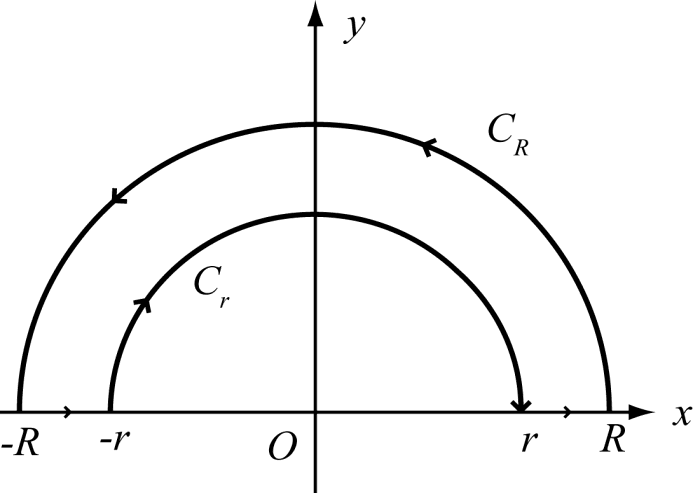
\includegraphics[keepaspectratio,alt={图5.4 避开原点的半圆周线}]{figures/05-留数理论及其应用/fig-p26-9e5100a0.png}}
\caption{图5.4 避开原点的半圆周线}
\end{figure}

在此周线中 \(f(z)\) 是解析的（\(z=0\)
已被小圆弧绕开），由柯西积分定理，得

\[
\int_{-R}^{-r}\frac{\mathrm e^{\mathrm i x}}{x}\,\mathrm dx
+\int_{C_r}\frac{\mathrm e^{\mathrm i z}}{z}\,\mathrm dz
+\int_{r}^{R}\frac{\mathrm e^{\mathrm i x}}{x}\,\mathrm dx
+\int_{C_R}\frac{\mathrm e^{\mathrm i z}}{z}\,\mathrm dz
=0 .
\]

令 \(x=-t\)，则有

\[
\int_{-R}^{-r}\frac{\mathrm e^{\mathrm i x}}{x}\,\mathrm dx
=-\int_{r}^{R}\frac{\mathrm e^{-\mathrm i t}}{t}\,\mathrm dt
=-\int_{r}^{R}\frac{\mathrm e^{-\mathrm i x}}{x}\,\mathrm dx .
\]

所以

\[
\int_{r}^{R}\frac{\mathrm e^{\mathrm i x}-\mathrm e^{-\mathrm i x}}{x}\,\mathrm dx
+\int_{C_R}\frac{\mathrm e^{\mathrm i z}}{z}\,\mathrm dz
+\int_{C_r}\frac{\mathrm e^{\mathrm i z}}{z}\,\mathrm dz
=0,
\]

即

\[
2\mathrm i\int_{r}^{R}\frac{\sin x}{x}\,\mathrm dx
+\int_{C_R}\frac{\mathrm e^{\mathrm i z}}{z}\,\mathrm dz
+\int_{C_r}\frac{\mathrm e^{\mathrm i z}}{z}\,\mathrm dz
=0 .
\]

由于

\[
\Bigl|\int_{C_R}\frac{\mathrm e^{\mathrm i z}}{z}\,\mathrm dz\Bigr|
\le\int_{0}^{\pi}\frac{\bigl|\mathrm e^{\mathrm i R\mathrm e^{\mathrm i\theta}}\bigr|}{R}\cdot R\,\mathrm d\theta
=\int_{0}^{\pi}\mathrm e^{-R\sin\theta}\,\mathrm d\theta
=2\int_{0}^{\pi/2}\mathrm e^{-R\sin\theta}\,\mathrm d\theta
\le\frac{\pi}{R}\bigl(1-\mathrm e^{-R}\bigr),
\]

故

\[
\lim_{R\to\infty}\int_{C_R}\frac{\mathrm e^{\mathrm i z}}{z}\,\mathrm dz=0 .
\]

又因为

\[
\frac{\mathrm e^{\mathrm i z}}{z}
=\frac{1}{z}+\mathrm i-\frac{z}{2!}+\cdots+\mathrm i^{n}\frac{z^{n-1}}{n!}+\cdots
=\frac{1}{z}+\varphi(z),
\]

其中 \(\varphi(z)\) 在 \(z=0\) 处解析，且
\(\varphi(0)=\mathrm i\)。因此当 \(|z|\) 充分小时，可设
\(|\varphi(z)|\le2\)。由于

\[
\int_{C_r}\frac{\mathrm e^{\mathrm i z}}{z}\,\mathrm dz
=\int_{C_r}\frac{\mathrm dz}{z}+\int_{C_r}\varphi(z)\,\mathrm dz,
\]

而

\[
\int_{C_r}\frac{\mathrm dz}{z}
=\int_{\pi}^{0}\frac{\mathrm i r\mathrm e^{\mathrm i\theta}}{r\mathrm e^{\mathrm i\theta}}\,\mathrm d\theta
=-\mathrm i\pi,
\qquad
\Bigl|\int_{C_r}\varphi(z)\,\mathrm dz\Bigr|\le2\pi r\to0,
\]

故有

\[
\lim_{r\to0}\int_{C_r}\frac{\mathrm e^{\mathrm i z}}{z}\,\mathrm dz=-\pi\mathrm i .
\]

令 \(R\to\infty\)，\(r\to0\)，则有

\[
2\mathrm i\int_{0}^{+\infty}\frac{\sin x}{x}\,\mathrm dx-\pi\mathrm i=0,
\]

即

\[
\boxed{\displaystyle\int_{0}^{+\infty}\frac{\sin x}{x}\,\mathrm dx=\frac{\pi}{2}} .
\]

\subsection{\texorpdfstring{5.2.4 形如
\(\displaystyle\int_{0}^{2\pi}R(\sin\theta,\cos\theta)\,\mathrm d\theta\)
的积分}{5.2.4 形如 \textbackslash displaystyle\textbackslash int\_\{0\}\^{}\{2\textbackslash pi\}R(\textbackslash sin\textbackslash theta,\textbackslash cos\textbackslash theta)\textbackslash,\textbackslash mathrm d\textbackslash theta 的积分}}\label{ux5f62ux5982-displaystyleint_02pirsinthetacosthetamathrm-dtheta-ux7684ux79efux5206}

设 \(R(x,y)\) 是两个变量 \(x,y\) 的有理函数。令
\(z=\mathrm e^{\mathrm i\theta}\)，那么

\[
\sin\theta=\frac{1}{2\mathrm i}\bigl(\mathrm e^{\mathrm i\theta}-\mathrm e^{-\mathrm i\theta}\bigr)
=\frac{1}{2\mathrm i}\Bigl(z-\frac{1}{z}\Bigr)
=\frac{z^{2}-1}{2\mathrm i z},
\]

\[
\cos\theta=\frac{1}{2}\bigl(\mathrm e^{\mathrm i\theta}+\mathrm e^{-\mathrm i\theta}\bigr)
=\frac{1}{2}\Bigl(z+\frac{1}{z}\Bigr)
=\frac{z^{2}+1}{2z},
\]

\[
\mathrm d\theta=\frac{\mathrm dz}{\mathrm i z}.
\]

从而原积分化为沿正向单位圆周的积分：

\[
\int_{0}^{2\pi}R(\cos\theta,\sin\theta)\,\mathrm d\theta
=\oint_{|z|=1}R\left(\frac{z^{2}+1}{2z},\frac{z^{2}-1}{2\mathrm i z}\right)\frac{\mathrm dz}{\mathrm i z}
=\oint_{|z|=1}f(z)\,\mathrm dz,
\]

其中 \(f(z)\) 为 \(z\) 的有理函数，且在单位圆周 \(|z|=1\) 上分母不为零。

\textbf{例 5.11} 计算积分

\[
\int_{0}^{2\pi}\cos^{4}4\theta\,\mathrm d\theta .
\]

\textbf{解} 令
\(z=\mathrm e^{\mathrm i\theta}\ (0\le\theta\le2\pi)\)，则

\[
\cos4\theta=\frac{z^{4}+z^{-4}}{2}=\frac{z^{8}+1}{2z^{4}},
\]

所以

\[
\begin{aligned}
\int_{0}^{2\pi}\cos^{4}4\theta\,\mathrm d\theta
&=\oint_{|z|=1}\left(\frac{z^{4}+z^{-4}}{2}\right)^{4}\frac{\mathrm dz}{\mathrm i z}
=\frac{1}{\mathrm i}\oint_{|z|=1}\frac{(z^{8}+1)^{4}}{16z^{17}}\,\mathrm dz .
\end{aligned}
\]

在 \(0<|z|<1\) 内，被积函数的洛朗展开式为

\[
\frac{(z^{8}+1)^{4}}{16z^{17}}
=\frac{1}{16}z^{-17}+\frac{1}{4}z^{-9}+\frac{3}{8}z^{-1}+\cdots.
\]

所以
\(operatorname{Res}\Bigl[\dfrac{(z^{8}+1)^{4}}{16z^{17}},0\Bigr]=\dfrac38\)，从而

\[
\int_{0}^{2\pi}\cos^{4}4\theta\,\mathrm d\theta
=\frac{1}{\mathrm i}\left\{2\pi\mathrm i\cdot\frac{3}{8}\right\}
=\frac{3}{4}\pi .
\]

\subsection{5.2.5 特殊定积分举例 II：Fresnel
积分}\label{ux7279ux6b8aux5b9aux79efux5206ux4e3eux4f8b-iifresnel-ux79efux5206}

由于留数是与闭曲线上的复积分相联系的，因此利用留数来计算定积分需要有两个主要的转化过程：

\begin{enumerate}
\def\labelenumi{\arabic{enumi}.}
\tightlist
\item
  将定积分的\textbf{被积函数}转化为复函数；
\item
  将定积分的\textbf{积分区间}转化为复积分的闭路曲线。
\end{enumerate}

下面用此方法计算积分

\[
\int_{0}^{\infty}\cos x^{2}\,\mathrm dx,\qquad
\int_{0}^{\infty}\sin x^{2}\,\mathrm dx .
\]

应取函数
\(f(z)=\mathrm e^{\mathrm i z^{2}}\)，取积分周线如图（扇形周线：\(OA\)
为实轴上 \(0\le x\le r\)，\(AB\) 为以原点为圆心、半径 \(r\)、辐角从
\(0\) 到 \(\pi/4\) 的圆弧，\(BO\) 为辐角 \(\pi/4\) 的径向线段）。

\begin{figure}
\centering
\pandocbounded{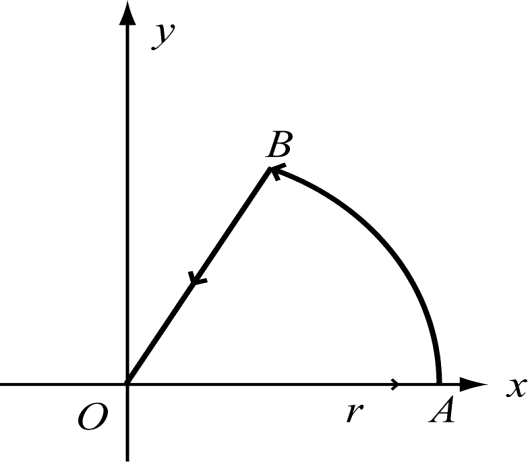
\includegraphics[keepaspectratio,alt={图5.5 计算 Fresnel 积分的扇形周线}]{figures/05-留数理论及其应用/fig-p31-29254dd8.png}}
\caption{图5.5 计算 Fresnel 积分的扇形周线}
\end{figure}

因为 \(f(z)\) 在闭周线内解析，由柯西积分定理，有

\[
\int_{OA}\mathrm e^{\mathrm i z^{2}}\,\mathrm dz
+\int_{AB}\mathrm e^{\mathrm i z^{2}}\,\mathrm dz
+\int_{BO}\mathrm e^{\mathrm i z^{2}}\,\mathrm dz
=0 .
\]

（1）当 \(z\) 在 \(OA\) 上时，\(z=x,\ 0\le x\le r\)，

\[
\int_{OA}\mathrm e^{\mathrm i z^{2}}\,\mathrm dz=\int_{0}^{r}\mathrm e^{\mathrm i x^{2}}\,\mathrm dx .
\]

（2）当 \(z\) 在 \(AB\)
上时，\(z=r\mathrm e^{\mathrm i\theta},\ 0\le\theta\le\dfrac{\pi}{4}\)，此时
\(\sin2\theta\ge\dfrac{4}{\pi}\theta\)，所以

\[
\bigl|\mathrm e^{\mathrm i z^{2}}\bigr|=\mathrm e^{-r^{2}\sin2\theta}\le\mathrm e^{-\frac{4}{\pi}r^{2}\theta},
\]

\[
\Bigl|\int_{AB}\mathrm e^{\mathrm i z^{2}}\,\mathrm dz\Bigr|
\le\int_{0}^{\pi/4}\mathrm e^{-\frac{4}{\pi}r^{2}\theta}\cdot r\,\mathrm d\theta
=\frac{\pi}{4r}\bigl(1-\mathrm e^{-r^{2}}\bigr)\to0\quad(r\to\infty).
\]

（3）当 \(z\) 在 \(BO\)
上时，\(z=x\mathrm e^{\mathrm i\pi/4},\ 0\le x\le r\)，则

\[
\int_{BO}\mathrm e^{\mathrm i z^{2}}\,\mathrm dz
=\int_{r}^{0}\mathrm e^{\mathrm i x^{2}\mathrm e^{\mathrm i\pi/2}}\cdot\mathrm e^{\mathrm i\pi/4}\,\mathrm dx
=-\mathrm e^{\mathrm i\pi/4}\int_{0}^{r}\mathrm e^{-x^{2}}\,\mathrm dx .
\]

令 \(r\to\infty\)，得

\[
\int_{0}^{\infty}\mathrm e^{\mathrm i x^{2}}\,\mathrm dx
+0-\mathrm e^{\mathrm i\pi/4}\int_{0}^{\infty}\mathrm e^{-x^{2}}\,\mathrm dx=0 .
\]

又

\[
\int_{0}^{\infty}\mathrm e^{-x^{2}}\,\mathrm dx=\frac{\sqrt\pi}{2},
\]

因此

\[
\int_{0}^{\infty}\mathrm e^{\mathrm i x^{2}}\,\mathrm dx
=\mathrm e^{\mathrm i\pi/4}\int_{0}^{\infty}\mathrm e^{-x^{2}}\,\mathrm dx
=\mathrm e^{\mathrm i\pi/4}\cdot\frac{\sqrt\pi}{2}.
\]

上式两边分别取实部和虚部，即得

\[
\boxed{\displaystyle\int_{0}^{\infty}\cos x^{2}\,\mathrm dx
=\int_{0}^{\infty}\sin x^{2}\,\mathrm dx
=\frac{1}{2}\sqrt{\frac{\pi}{2}}
=\frac{\sqrt{2\pi}}{4}} .
\]

\begin{quote}
\textbf{注} 幻灯片最后一行为
\(\dfrac12\cdot\dfrac{\sqrt\pi}{2}=\dfrac{\sqrt\pi}{4}\)，这是笔误。正确的应为
\(\dfrac12\sqrt{\dfrac{\pi}{2}}=\dfrac{\sqrt{2\pi}}{4}\)。
\end{quote}

\subsection{常见错误与注意点}\label{ux5e38ux89c1ux9519ux8befux4e0eux6ce8ux610fux70b9-13}

\begin{enumerate}
\def\labelenumi{\arabic{enumi}.}
\tightlist
\item
  \textbf{用 \(\int R(x)\mathrm dx\) 公式前必须验证
  \(n-m\ge2\)}。若只差一次，圆弧积分不一定为 \(0\)，此时要用含
  \(\mathrm e^{\alpha\mathrm i x}\) 的公式（\(n-m\ge1\)）。
\item
  \textbf{只取上半平面的极点}。留数求和只对 \(C_r\)
  内部的极点进行；实轴上的极点需另作处理（一般用小圆弧绕过）。
\item
  \textbf{Jordan 不等式}：当 \(0\le\theta\le\pi/2\) 时
  \(\sin\theta\ge\dfrac{2\theta}{\pi}\)。估算
  \(\displaystyle\int_0^{\pi/2}\mathrm e^{-\alpha r\sin\theta}\mathrm d\theta\)
  时，结果应为
  \(\dfrac{M\pi}{\alpha r}(1-\mathrm e^{-\alpha r})\)；幻灯片写成了
  \(\dfrac{M\pi}{2r}(1-\mathrm e^{-\alpha r})\)，漏掉了 \(\alpha\)。
\item
  \textbf{含 \(\mathrm e^{\alpha\mathrm i x}\)
  的积分常分开实、虚部求值}。例如例 5.9
  中，\(\int\cos x/(x^2+4x+5)\mathrm dx=\operatorname{Re}[\pi\mathrm e^{-1-2\mathrm i}]=\pi\mathrm e^{-1}\cos2\)，不要忘记取实部。
\item
  \textbf{例 5.8
  的乘子``\(2\pi\mathrm i\)''不要写成``\(2\pi\)''}。幻灯片写
  \(2\pi\left(\cdots\right)\) 是漏了 \(\mathrm i\)；严格应为
  \(2\pi\mathrm i\sum\operatorname{Res}\)。另外，幻灯片把这两个留数写成
  \(\dfrac{1+\mathrm i}{4\sqrt2\,\mathrm i}\) 与
  \(\dfrac{1-\mathrm i}{4\sqrt2\,\mathrm i}\)，等价于
  \(\dfrac{1-\mathrm i}{4\sqrt2}\) 与
  \(-\dfrac{1+\mathrm i}{4\sqrt2}\)。
\item
  \textbf{\(\sin x/x\) 的周线要避开原点}。因为 \(z=0\)
  是被积函数的可去奇点，周线必须用小圆弧绕开，且小圆弧积分
  \(\to-\pi\mathrm i\)。\(\lim_{r\to0}\int_{C_r}\mathrm e^{\mathrm i z}/z\,\mathrm dz=-\pi\mathrm i\)
  的符号很关键。
\item
  \textbf{Fresnel
  积分结果}：\(\int_0^\infty\cos x^2\mathrm dx=\int_0^\infty\sin x^2\mathrm dx=\dfrac12\sqrt{\dfrac{\pi}{2}}=\dfrac{\sqrt{2\pi}}{4}\)。不要把幻灯片中的
  \(\dfrac{\sqrt\pi}{4}\) 当成正确结果。
\end{enumerate}

\subsection{本节小结}\label{ux672cux8282ux5c0fux7ed3-13}

\begin{itemize}
\tightlist
\item
  \textbf{无理函数无穷积分}
  \(\int_{-\infty}^{\infty}R(x)\mathrm dx\)（\(n-m\ge2\)，\(Q\)
  无实零点）：取上半平面半圆，\(R\) 在圆弧上为
  \(O(|z|^{-2})\)，故圆弧积分趋于 \(0\)，结果是
  \(2\pi\mathrm i\sum\operatorname{Res}[R,z_k]\)（\(z_k\) 在上半平面）。
\item
  \textbf{含 \(\mathrm e^{\alpha\mathrm i x}\)
  的积分}（\(\alpha>0\)，\(n-m\ge1\)）：用 Jordan 不等式估计圆弧，结果
  \(2\pi\mathrm i\sum\operatorname{Res}[R\mathrm e^{\alpha\mathrm i z},z_k]\)；\(\alpha i\)
  的实部为负保证上半圆弧被``压''到 \(0\)。
\item
  \textbf{三角有理式周期积分}
  \(\int_0^{2\pi}R(\sin\theta,\cos\theta)\mathrm d\theta\)：令
  \(z=\mathrm e^{\mathrm i\theta}\)，化为单位圆周上的复积分
  \(\oint_{|z|=1}f(z)\mathrm dz\)。
\item
  \textbf{特殊定积分}：\(\int_0^\infty\frac{\sin x}{x}\mathrm dx=\frac{\pi}{2}\)；\(\int_0^\infty\cos x^2\mathrm dx=\int_0^\infty\sin x^2\mathrm dx=\frac{\sqrt{2\pi}}{4}\)。
\item
  核心思想：\textbf{用留数定理计算实定积分时，关键是``选对周线、让非待求部分趋于零、把待求部分与留数联系起来''}。
\end{itemize}

\newpage

\chaptercover{6}{共形映射}
%% 由 build/emit_tex.py 生成（生成物，勿手改）；定制请放 user_style.tex / user_meta.yaml
\chapter{第 6 章 ·
共形映射}\label{ux7b2c-6-ux7ae0-ux5171ux5f62ux6620ux5c04}

\section{6.1 分式线性变换}\label{ux5206ux5f0fux7ebfux6027ux53d8ux6362}

\begin{quote}
本节目标：理解分式线性变换的定义及其``保广义圆、保交比、保角''等基本性质，掌握由三个对应点唯一确定分式线性变换的方法，并能把单位圆、上半平面、角域等简单区域互相映射。
重点：分式线性变换的定义与分解；保广义圆定理；交比不变性；单位圆与上半平面互映。
难点：无穷远点的处理；广义圆（圆与直线）的统一；交比的符号与使用；判断像曲线是圆还是直线。
\end{quote}

\subsection{6.1.1
分式线性变换的定义}\label{ux5206ux5f0fux7ebfux6027ux53d8ux6362ux7684ux5b9aux4e49}

\textbf{定义 6.1} 形如

\[
w = \frac{az+b}{cz+d},\qquad a,b,c,d \in \mathbb{C},\quad ad-bc \neq 0
\]

的函数称为\textbf{分式线性变换}（又称\textbf{双线性变换}或
\textbf{Möbius 变换}），其中 \(z\) 与 \(w\) 都在扩充复平面

\[
\mathbb{C}_{\infty} = \mathbb{C}\cup\{\infty\}
\]

上取值。常数矩阵

\[
\begin{pmatrix} a & b \\ c & d \end{pmatrix}
\]

称为该变换的\textbf{矩阵}，它与原矩阵相差一个非零常数因子时对应同一个变换。

几点说明：

\begin{itemize}
\tightlist
\item
  当 \(c=0\)
  时，\(w=\dfrac{a}{d}z+\dfrac{b}{d}\)，是通常的\textbf{线性（整线性）变换}，即平移、旋转与伸缩的复合。
\item
  当 \(c\neq 0\) 时，分母为零的点 \(z=-\dfrac{d}{c}\) 映为无穷远点
  \(\infty\)；而 \(z=\infty\) 则映为 \(w=\dfrac{a}{c}\)。
\item
  由于
  \(ad-bc\neq 0\)，分式线性变换在扩充复平面上是\textbf{一一对应（双射）}，因而是单叶的：它把
  \(\mathbb{C}_{\infty}\) 整个地且双方单值地映为自身。
\end{itemize}

\textbf{定义 6.2} 在扩充复平面 \(\mathbb{C}_{\infty}\)
上，\textbf{圆}与\textbf{直线}统称为\textbf{广义圆}（也称``圆周''）。这是因为直线可以看成通过无穷远点
\(\infty\) 的``半径为无穷大的圆''。

\begin{quote}
配图：建议绘制一条不经原点的直线与一个不经过原点的圆，再分别画出
\(w=1/z\) 后的像，直观展示``直线映圆、圆映圆''的保广义圆性。
\end{quote}

\subsection{6.1.2
分式线性变换的分解}\label{ux5206ux5f0fux7ebfux6027ux53d8ux6362ux7684ux5206ux89e3}

\textbf{性质 6.1} 任一非恒等的分式线性变换
\(w=\dfrac{az+b}{cz+d}\)（\(ad-bc\neq 0\)）都可分解为下列三类简单变换的复合：

\begin{enumerate}
\def\labelenumi{\arabic{enumi}.}
\tightlist
\item
  \textbf{平移}：\(w=z+b\)；
\item
  \textbf{旋转与伸缩（相似变换）}：\(w=az\)，\(a\neq 0\)；
\item
  \textbf{反演}：\(w=\dfrac{1}{z}\)。
\end{enumerate}

具体地，当 \(c\neq 0\) 时，

\[
w = \frac{az+b}{cz+d}
= \frac{a}{c} + \frac{bc-ad}{c}\cdot\frac{1}{cz+d}.
\]

若令
\(w_1=cz+d\)（相似变换），\(w_2=\dfrac{1}{w_1}\)（反演），\(w_3=\dfrac{bc-ad}{c}w_2+\dfrac{a}{c}\)（伸缩加平移），则
\(w=w_3\)。

\textbf{结论}
研究分式线性变换的几何性质，只需研究平移、旋转伸缩与反演这三种基本变换；这也为下述保广义圆性提供了证明思路。

\subsection{6.1.3 保广义圆性}\label{ux4fddux5e7fux4e49ux5706ux6027}

\textbf{定理 6.1（保广义圆性）} 分式线性变换把 \(\mathbb{C}_{\infty}\)
上的广义圆映为广义圆。即：圆或直线经分式线性变换后仍是圆或直线。并且它把圆（或直线）的内部（或一侧半平面）映为像圆（或直线）的内部或外部（或另一侧半平面）。

\textbf{证明思路} 平移与旋转伸缩显然把广义圆映为广义圆。因此只需证明反演
\(w=1/z\) 保持广义圆。任取一个广义圆，其方程可写成

\[
A z\bar z + \bar B z + B \bar z + C = 0,\qquad A,C \in \mathbb{R},
\]

其中 \(A=0\) 时表示直线，\(A\neq 0\) 时表示圆。令
\(z=\dfrac{1}{w}\)，代入并乘以 \(w\bar w\)，得

\[
A + \bar B \bar w + B w + C w\bar w = 0,
\]

仍是同类型的广义圆方程，故 \(w=1/z\) 保广义圆。由性质 6.1
的分解，任一非恒等分式线性变换都保广义圆。\(\square\)

\textbf{重要判别}
一条直线经过分式线性变换后，何时仍为直线、何时变为圆？原则是：\textbf{若原直线（或圆）经过极点
\(z=-d/c\)，则像为直线；否则像为圆}。更一般地，广义圆像的类型取决于极点是否落在该广义圆上。

\subsection{6.1.4
交比及其不变性}\label{ux4ea4ux6bd4ux53caux5176ux4e0dux53d8ux6027}

\textbf{定义 6.3（交比）} 设 \(z_1,z_2,z_3,z_4\)
是扩充复平面上四个互异的点，称

\[
(z_1,z_2;z_3,z_4)
= \frac{z_1-z_3}{z_1-z_4}\Big/\frac{z_2-z_3}{z_2-z_4}
= \frac{(z_1-z_3)(z_2-z_4)}{(z_1-z_4)(z_2-z_3)}
\]

为这四个点的\textbf{交比}。若其中有无穷远点，则按下列极限理解：

\[
(\infty, z_2; z_3, z_4)=\frac{z_2-z_4}{z_2-z_3},\qquad
(z_1, \infty; z_3, z_4)=\frac{z_1-z_3}{z_1-z_4}.
\]

\textbf{定理 6.2（交比不变性）} 设 \(w=L(z)\)
是一个分式线性变换，\(z_j\)（\(j=1,2,3,4\)）为四个点，\(w_j=L(z_j)\)，则

\[
(w_1,w_2;w_3,w_4) = (z_1,z_2;z_3,z_4).
\]

即\textbf{交比是分式线性变换下的不变量}。

\textbf{证明思路} 由性质 6.1，只需对平移、旋转伸缩和反演 \(w=1/z\)
逐一验证交比不变；直接代入交比定义即可。\(\square\)

\textbf{性质 6.2（四点共圆的判据）} \(z_1,z_2,z_3,z_4\) 在
\(\mathbb{C}_{\infty}\) 上共圆或共线的充要条件是：它们的交比
\((z_1,z_2;z_3,z_4)\) 为实数。

\textbf{说明}
因为存在唯一的分式线性变换把前三点映为实轴上的三点，而交比不变；实轴上（共线）四点的交比为实数；反之亦然。这一判据是处理``四点共圆''类问题的重要工具。

\subsection{6.1.5
由三对对应点确定变换}\label{ux7531ux4e09ux5bf9ux5bf9ux5e94ux70b9ux786eux5b9aux53d8ux6362}

\textbf{定理 6.3} 在扩充复平面上任意给定三个互异的点 \(z_1,z_2,z_3\)
与三个互异的点 \(w_1,w_2,w_3\)，存在\textbf{唯一}的分式线性变换
\(w=L(z)\)，使得

\[
L(z_1)=w_1,\qquad L(z_2)=w_2,\qquad L(z_3)=w_3 .
\]

并且该变换可由交比相等直接写出：

\[
\frac{w-w_1}{w-w_2}\cdot\frac{w_3-w_2}{w_3-w_1}
=
\frac{z-z_1}{z-z_2}\cdot\frac{z_3-z_2}{z_3-z_1}.
\]

若某点为无穷远点，则把含有该点的因子按``消去''处理（例如含 \(\infty\)
的差项省略或取极限）。

\textbf{证明思路} 上式右端是 \(z\) 的分式线性函数，且在
\(z=z_1,z_2,z_3\) 时分别取 \(0,\infty,1\)，从而左端的 \(w\) 分别在
\(w_1,w_2,w_3\) 处取相应值；由解的唯一性即得。\(\square\)

\textbf{推论}
分式线性变换把由三点确定的广义圆映为由对应三点确定的广义圆。

\subsection{6.1.6
单位圆与上半平面之间的映射}\label{ux5355ux4f4dux5706ux4e0eux4e0aux534aux5e73ux9762ux4e4bux95f4ux7684ux6620ux5c04}

以下两个映射是本章最常用的``标准区域互映''：

\textbf{上半平面到单位圆盘：}

\[
w = \frac{z-i}{z+i}
\]

把 \(\operatorname{Im}z>0\) 共形地映为 \(|w|<1\)，把实轴映为单位圆，且
\(z=i\) 映为 \(w=0\)。

\textbf{单位圆盘到上半平面：}

\[
w = i\frac{1+z}{1-z}
\]

把 \(|z|<1\) 共形地映为 \(\operatorname{Im}w>0\)，把单位圆映为实轴，且
\(z=0\) 映为 \(w=i\)。

\begin{quote}
配图：建议在上半平面画一条水平直线（表示实轴）与半径为 1
的圆，分别用箭头表示 \(w=(z-i)/(z+i)\) 与 \(w=i(1+z)/(1-z)\)
的对应关系。
\end{quote}

\subsection{6.1.7 典型例题}\label{ux5178ux578bux4f8bux9898-2}

\textbf{例 6.1} 求分式线性变换 \(w=L(z)\)，使
\(L(0)=\infty\)，\(L(1)=i\)，\(L(\infty)=0\)。

\textbf{解} 利用定理 6.3。取
\(z_1=0,w_1=\infty\)；\(z_2=1,w_2=i\)；\(z_3=\infty,w_3=0\)。由交比相等

\[
(w,\infty;i,0)=(z,0;1,\infty),
\]

其中左端（因含 \(\infty\)，令 \(z_2\to\infty\) 取极限）为
\(\dfrac{w-i}{w}\)，右端（令 \(z_4\to\infty\) 取极限）为
\(\dfrac{z-1}{0-1}=1-z\)。于是

\[
\frac{w-i}{w}=1-z
\quad\Longrightarrow\quad
w-i=w(1-z)
\quad\Longrightarrow\quad
wz=i
\quad\Longrightarrow\quad
w=\frac{i}{z}.
\]

故所求变换为 \(w=\dfrac{i}{z}\)。验证：\(z=0\) 时 \(w=\infty\)；\(z=1\)
时 \(w=i\)；\(z=\infty\) 时 \(w=0\)。\(\blacksquare\)

\textbf{例 6.2} 求把单位圆盘 \(|z|<1\) 映射为上半平面
\(\operatorname{Im}w>0\)，且把 \(z=0\) 映为 \(w=i\) 的分式线性变换。

\textbf{解} 取

\[
w = i\frac{1+z}{1-z}.
\]

当 \(z=0\) 时，\(w=i\)，满足条件。下面验证它把单位圆映为实轴。设
\(z=e^{i\theta}\)（\(|z|=1\)），则

\[
\frac{1+e^{i\theta}}{1-e^{i\theta}}
= \frac{2\cos\frac{\theta}{2}\,e^{i\theta/2}}
{-2i\sin\frac{\theta}{2}\,e^{i\theta/2}}
= i\cot\frac{\theta}{2},
\]

于是

\[
w = i\cdot i\cot\frac{\theta}{2} = -\cot\frac{\theta}{2}\in \mathbb{R}.
\]

故单位圆映为实轴。又因 \(z=0\) 映为
\(w=i\)（在上半平面），且分式线性变换是单叶双射，故单位圆盘内部映为上半平面。所求变换为

\[
\boxed{\;w=i\frac{1+z}{1-z}\;}.
\]

（若要求``上半平面到单位圆盘''，则可取
\(w=\dfrac{z-i}{z+i}\)。）\(\blacksquare\)

\textbf{例 6.3} 求 \(w=\dfrac{1}{z}\) 把直线 \(x=1\) 映成什么曲线。

\textbf{解} 直线 \(x=1\) 上的点可写为
\(z=1+iy\)（\(y\in\mathbb{R}\)）。于是

\[
w=\frac{1}{1+iy}=\frac{1-iy}{1+y^2}.
\]

令 \(w=u+iv\)，则

\[
u=\frac{1}{1+y^2},\qquad v=\frac{-y}{1+y^2}.
\]

消去 \(y\)：因为

\[
u^2+v^2=\frac{1+y^2}{(1+y^2)^2}=\frac{1}{1+y^2}=u,
\]

所以

\[
u^2+v^2=u
\quad\Longleftrightarrow\quad
\left(u-\frac12\right)^{2}+v^{2}=\left(\frac12\right)^{2}.
\]

即 \(w=\dfrac{1}{z}\) 把直线 \(x=1\) 映为以 \(\dfrac12\)
为圆心、\(\dfrac12\) 为半径的圆。由于直线 \(x=1\) 不经过极点
\(z=0\)，故像为圆而非直线。\(\blacksquare\)

\subsection{常见错误与注意点}\label{ux5e38ux89c1ux9519ux8befux4e0eux6ce8ux610fux70b9-18}

\begin{enumerate}
\def\labelenumi{\arabic{enumi}.}
\tightlist
\item
  \textbf{忘记
  \(ad-bc\neq 0\)}：若为零，变换退化（如分子分母成比例），不再是双射，不满足分式线性变换的要求。
\item
  \textbf{无穷远点的处理}：\(z=-d/c\) 映为 \(\infty\)，\(z=\infty\) 映为
  \(a/c\)（\(c=0\) 时映为 \(\infty\)）。不要把 \(\infty\)
  当普通复数值直接代入。
\item
  \textbf{``圆还是直线''的判断}：像曲线是圆还是直线，取决于极点
  \(z=-d/c\) 是否在原广义圆上。必须养成先看极点位置的习惯。
\item
  \textbf{交比顺序}：交比 \((z_1,z_2;z_3,z_4)\)
  对位置的顺序敏感，交换点会改变数值甚至变为倒数；使用时要保持一致。
\item
  \textbf{单位圆与上半平面映射不唯一}：只给``区域对应''不能唯一确定变换，还需再给``三个点对''之类条件（如
  \(z=0\mapsto i\)）才能唯一确定。
\item
  \textbf{方向相反}：\(w=(z-i)/(z+i)\) 是``上半平面→单位圆''，而
  \(w=i(1+z)/(1-z)\) 是``单位圆→上半平面''，不要颠倒。
\end{enumerate}

\subsection{本节小结}\label{ux672cux8282ux5c0fux7ed3-18}

\begin{itemize}
\tightlist
\item
  \textbf{定义}：分式线性变换
  \(w=\frac{az+b}{cz+d}\)（\(ad-bc\neq0\)）是扩充复平面上的单叶双射。
\item
  \textbf{分解}：平移、旋转伸缩与反演；由此可证``保广义圆''。
\item
  \textbf{保广义圆}：圆或直线映为圆或直线；判别像为圆还是直线看极点是否落在原曲线上。
\item
  \textbf{交比}：\((z_1,z_2;z_3,z_4)\)
  在分式线性变换下不变；四点为实数交比当且仅当四点共圆或共线。
\item
  \textbf{三点定变换}：给定三对对应点唯一确定一个分式线性变换。
\item
  \textbf{标准映射}：\(w=\frac{z-i}{z+i}\)（上半平面→单位圆）、\(w=i\frac{1+z}{1-z}\)（单位圆→上半平面）。
\end{itemize}

\section{6.2 共形映射}\label{ux5171ux5f62ux6620ux5c04}

\begin{quote}
本节目标：理解导数的几何意义（伸缩率与旋转角），掌握共形映射（保角映射）的定义与判定，了解共形映射的局部单叶性、区域对应与边界对应等基本性质。
重点：导数的几何意义；共形映射的定义与判定条件（\(f'(z)\neq 0\)）；共形映射的局部单叶性与可逆性。
难点：夹角``大小与方向''的双重保持；导数零点处角度的``放大倍数''；单叶（一一）与局部共形的区别。
\end{quote}

\subsection{6.2.1
曲线的切线与两曲线的夹角}\label{ux66f2ux7ebfux7684ux5207ux7ebfux4e0eux4e24ux66f2ux7ebfux7684ux5939ux89d2}

设曲线 \(\Gamma\) 的参数方程为

\[
z=z(t)=x(t)+iy(t),\qquad a\le t\le b,
\]

且 \(z'(t_0)\neq 0\)。则 \(\Gamma\) 在 \(z_0=z(t_0)\) 处的切线方向向量为
\(z'(t_0)\)，其方向角（切线的辐角）为

\[
\arg z'(t_0).
\]

设两条曲线 \(\Gamma_1,\Gamma_2\) 在 \(z_0=z_1(t_0)=z_2(t_0)\) 处相交，且
\(z_1'(t_0)\neq 0\)，\(z_2'(t_0)\neq 0\)。规定它们的\textbf{夹角}为两切线方向的有向夹角：

\[
\angle(\Gamma_1,\Gamma_2) = \arg z_2'(t_0) - \arg z_1'(t_0).
\]

\begin{quote}
配图：建议画出两条曲线在交点 \(z_0\) 处的切线，标明夹角
\(\theta\)，以及映射后两条像曲线在 \(w_0=f(z_0)\) 处的夹角仍为
\(\theta\)。
\end{quote}

\subsection{6.2.2
导数的几何意义：伸缩率与旋转角}\label{ux5bfcux6570ux7684ux51e0ux4f55ux610fux4e49ux4f38ux7f29ux7387ux4e0eux65cbux8f6cux89d2}

\textbf{定理 6.4（导数的几何意义）} 设 \(f(z)\) 在 \(z_0\) 处解析，且
\(f'(z_0)\neq 0\)。过 \(z_0\) 的任意曲线 \(\Gamma\)（参数方程
\(z=z(t)\)，\(z(t_0)=z_0\)，\(z'(t_0)\neq 0\)）在映射 \(w=f(z)\)
下的像曲线 \(\Gamma'=f(\Gamma)\)，在 \(w_0=f(z_0)\) 处的切线方向满足

\[
\arg w'(t_0) = \arg f'(z_0) + \arg z'(t_0).
\]

由此得到两个与曲线形状无关的常数：

\begin{enumerate}
\def\labelenumi{\arabic{enumi}.}
\tightlist
\item
  \textbf{伸缩率}：像曲线在 \(w_0\) 处的切向量长度为原曲线切向量长度的
  \(|f'(z_0)|\) 倍，即 \[
  |f'(z_0)| = \text{放大倍数},
  \] 只与点 \(z_0\) 有关；
\item
  \textbf{旋转角}：每一条过 \(z_0\) 的曲线，其切线方向都旋转同一个角 \[
  \arg f'(z_0),
  \] 也与曲线形状无关。
\end{enumerate}

\textbf{证明} 由复合函数求导法则，像曲线为
\(w=w(t)=f\bigl(z(t)\bigr)\)，故

\[
w'(t_0)=f'\bigl(z(t_0)\bigr)\,z'(t_0)=f'(z_0)\,z'(t_0).
\]

取辐角得 \(\arg w'(t_0)=\arg f'(z_0)+\arg z'(t_0)\)，取模得
\(|w'(t_0)|=|f'(z_0)|\,|z'(t_0)|\)。\(\square\)

\subsection{6.2.3
共形映射的定义与判定}\label{ux5171ux5f62ux6620ux5c04ux7684ux5b9aux4e49ux4e0eux5224ux5b9a}

\textbf{定义 6.4（共形映射）} 设 \(f(z)\) 在 \(z_0\)
的一个邻域内解析。若映射 \(w=f(z)\) 在 \(z_0\)
处保持两条曲线夹角的\textbf{大小}和\textbf{方向}不变，并且在该点有确定的伸缩率
\(|f'(z_0)|\)，则称 \(w=f(z)\) 在 \(z_0\)
处是\textbf{共形映射}（又称\textbf{保角映射}）。若 \(f\) 在区域 \(D\)
内每一点都共形，则称 \(f\) 在 \(D\) 内是\textbf{共形映射}。

由定理 6.4，当 \(f'(z_0)\neq 0\) 时，映射在 \(z_0\)
处不仅保持夹角，而且伸缩率与旋转角均为常数，因此是共形的。

\textbf{定理 6.5（共形映射的判定）} 设 \(f(z)\) 是区域 \(D\)
内的单值解析函数。则 \(f\) 在 \(D\) 内共形的充要条件是

\[
f'(z)\neq 0,\qquad \forall\, z\in D .
\]

\textbf{性质 6.3（导数零点处不保角）} 若 \(f'(z_0)=0\)，则 \(w=f(z)\) 在
\(z_0\) 处不是共形的。更一般地，若

\[
f(z)=(z-z_0)^{n}\,g(z),\qquad g(z_0)\neq 0,\quad n\ge 2,
\]

即 \(f\) 在 \(z_0\) 处有 \(n\) 阶零点，则映射在 \(z_0\)
处把任意两条曲线的夹角放大为原来的 \(n\) 倍：

\[
\angle\left(f(\Gamma_1),f(\Gamma_2)\right)=n\,\angle(\Gamma_1,\Gamma_2).
\]

例如 \(w=z^2\) 在 \(z=0\) 处 \(f'(0)=0\)，夹角被放大为原来的 \(2\)
倍，故 \(z=0\) 不是共形点。

\textbf{说明}
这里``共形''强调\textbf{保角}（保夹角的大小与方向）。若只保夹角大小而不保方向（如反演后取共轭），则称为``保角但反定向''；本书约定共形映射保持夹角方向不变。

\subsection{6.2.4
共形映射的主要性质}\label{ux5171ux5f62ux6620ux5c04ux7684ux4e3bux8981ux6027ux8d28}

\textbf{定义 6.5（单叶函数）} 设 \(f(z)\) 在区域 \(D\) 内解析。若对任意
\(z_1\neq z_2\in D\)，都有 \(f(z_1)\neq f(z_2)\)，则称 \(f\) 是 \(D\)
上的\textbf{单叶函数}（又称一一解析函数）。

\textbf{定理 6.6（局部单叶与解析反函数）} 设 \(f\) 在 \(z_0\) 处解析且
\(f'(z_0)\neq 0\)，则存在 \(z_0\) 的邻域，使 \(f\)
在该邻域内单叶，且反函数 \(z=f^{-1}(w)\) 在 \(w_0=f(z_0)\)
的某邻域内解析，并且

\[
\left(f^{-1}\right)'(w_0)=\frac{1}{f'(z_0)} .
\]

因此 \(f^{-1}\) 在 \(w_0\) 处也是共形的。

\textbf{证明要点} 由解析函数的反函数定理（或由 Cauchy--Riemann
方程推得的雅可比行列式 \(J=|f'(z)|^{2}\)
非零）即可得到局部单叶与反函数的解析性。\(\square\)

\textbf{定理 6.7（开映射与区域对应）} 若 \(f\) 在区域 \(D\)
内解析且不恒为常数，则 \(f(D)\)
是开集（\textbf{开映射定理}），因此非恒常解析函数把区域映为区域。若
\(f\) 是 \(D\) 上的单叶函数，则 \(f\) 把 \(D\)
共形地、双方单值地映为区域 \(f(D)\)，且 \(f^{-1}\) 也在 \(f(D)\)
上共形。

\textbf{性质 6.4（边界对应）} 设 \(f\) 把一个简单的单连通区域 \(D\)
共形地、单叶地映为另一个单连通区域 \(D'\)，且 \(f\) 可连续延拓到 \(D\)
的边界
\(\partial D\)，则边界点映为边界点，且边界的方向保持（保持边界定向）。这是解决``区域映射为简单区域''类问题的理论依据。

\textbf{性质 6.5（复合的共形性）} 若 \(w=f(z)\) 在 \(z_0\)
处共形，\(\zeta=g(w)\) 在 \(w_0=f(z_0)\) 处共形，则复合映射
\(\zeta=g\bigl(f(z)\bigr)\) 在 \(z_0\) 处共形，且

\[
\bigl(g\circ f\bigr)'(z_0)=g'\bigl(f(z_0)\bigr)\,f'(z_0)\neq 0 .
\]

这说明共形映射可以``复合''，这也是 6.3
节中把复杂区域逐级化为简单区域的基本手段。

\subsection{6.2.5 典型例题}\label{ux5178ux578bux4f8bux9898-3}

\textbf{例 6.4} 设 \(w=z^2\)。研究它在 \(z_0=1+i\)
处的伸缩率与旋转角，并说明在 \(z=0\) 处是否共形。

\textbf{解}

\[
f'(z)=2z,\qquad f'(1+i)=2(1+i)=2+2i .
\]

于是

\[
|f'(1+i)|=|2+2i|=2\sqrt2,\qquad
\arg f'(1+i)=\arg(2+2i)=\frac{\pi}{4}.
\]

即映射 \(w=z^2\) 在 \(z_0=1+i\) 处的伸缩率为
\(2\sqrt2\)，任何过该点的曲线其切线方向都旋转
\(\dfrac{\pi}{4}\)（\(45^\circ\)）。又 \(f'(0)=0\)，故 \(w=z^2\) 在
\(z=0\) 处不是共形的（夹角被放大为原来的 \(2\) 倍）。\(\blacksquare\)

\textbf{例 6.5} 证明 \(w=\dfrac{1}{z}\) 在 \(z\neq 0\) 处处处共形。

\textbf{解}

\[
f'(z)=-\frac{1}{z^{2}},\qquad z\neq 0 .
\]

对一切 \(z\neq 0\)，\(f'(z)\neq 0\)，且 \(f\) 在 \(z\neq 0\)
处解析，故由定理 6.5，\(w=\dfrac{1}{z}\) 在 \(z\neq 0\)
处处处共形。例如在 \(z_0=1+i\) 处，

\[
f'(1+i)=-\frac{1}{(1+i)^{2}}=-\frac{1}{2i}=\frac{i}{2},
\]

故伸缩率为 \(\left|\dfrac{i}{2}\right|=\dfrac12\)，旋转角为
\(\arg\dfrac{i}{2}=\dfrac{\pi}{2}\)。\(\blacksquare\)

\textbf{例 6.6} 求 \(w=z^2\) 把第一象限
\(\left\{0<\arg z<\dfrac{\pi}{2}\right\}\)
映射成的区域，并说明是否为共形的一一映射。

\textbf{解} 设 \(z=re^{i\theta}\)，\(0<\theta<\dfrac{\pi}{2}\)，则

\[
w=z^{2}=r^{2}e^{i2\theta}.
\]

于是 \(\arg w=2\theta\in(0,\pi)\)，\(|w|=r^{2}>0\)。故像区域为上半平面

\[
\operatorname{Im}w>0 .
\]

由于在第一象限内 \(f'(z)=2z\neq 0\)，且扇形角
\(\dfrac{\pi}{2}\le \pi\)，\(z^2\) 后角度为 \(\pi\)，仍在 \(2\pi\)
范围内，故映射是单叶的，于是 \(w=z^2\)
把第一象限共形地、一一地映为上半平面。\(\blacksquare\)

\subsection{常见错误与注意点}\label{ux5e38ux89c1ux9519ux8befux4e0eux6ce8ux610fux70b9-19}

\begin{enumerate}
\def\labelenumi{\arabic{enumi}.}
\tightlist
\item
  \textbf{混淆``解析''与``共形''}：解析函数只有在导数不为零处才保角；\(w=z^2\)
  在 \(z=0\) 解析但不共形。
\item
  \textbf{忽略旋转方向}：夹角是``有向''的，\(\angle(\Gamma_1,\Gamma_2)=\arg z_2'-\arg z_1'\)；方向颠倒则角度反号。
\item
  \textbf{把局部共形当作整体单叶}：\(f'(z)\neq 0\)
  在全域成立只能保证``局部单叶''，不保证整体一一。例如 \(w=e^z\) 处处
  \(f'\neq0\)，但不是整体单叶（有周期 \(2\pi i\)）。
\item
  \textbf{误用反函数导数}：\((f^{-1})'(w_0)=1/f'(z_0)\)，不要写成
  \(f'(z_0)\)。
\item
  \textbf{混淆``角域''与``半平面''的映射}：通过复合把角域、带形区域化为上半平面或单位圆时，要逐步检查每一步是否共形、是否单叶。
\end{enumerate}

\subsection{本节小结}\label{ux672cux8282ux5c0fux7ed3-19}

\begin{itemize}
\tightlist
\item
  \textbf{导数的几何意义}：\(|f'(z_0)|\) 为伸缩率，\(\arg f'(z_0)\)
  为旋转角，二者均与曲线形状无关。
\item
  \textbf{共形映射}：保夹角大小与方向的映射；\(f\) 解析且 \(f'(z)\neq0\)
  是共形的充要条件。
\item
  \textbf{导数零点}：\(n\) 阶零点处夹角放大 \(n\) 倍，不共形。
\item
  \textbf{重要性质}：局部单叶与解析反函数；开映射与区域对应；边界对应；复合共形。
\item
  \textbf{例题}：\(w=z^2\)、\(w=1/z\) 的共形性分析与区域映射。
\end{itemize}

\section{6.3
几个初等函数所构成的映射}\label{ux51e0ux4e2aux521dux7b49ux51fdux6570ux6240ux6784ux6210ux7684ux6620ux5c04}

\begin{quote}
本节目标：掌握幂函数 \(w=z^n\) 与指数函数 \(w=e^z\)
的共形性及其区域映射规律，能利用它们（常与分式线性变换复合）把角域、带形区域映射为半平面或单位圆。
重点：幂函数把``角域→角域（角度放大 \(n\)
倍）''；指数函数把``带形区域→角域、带形→半平面''；单叶条件与复合映射。
难点：单叶（一一）区域的选取；周期性与分支问题；把复杂区域逐级化为简单区域。
\end{quote}

\subsection{\texorpdfstring{6.3.1 幂函数
\(w=z^n\)}{6.3.1 幂函数 w=z\^{}n}}\label{ux5e42ux51fdux6570-wzn}

\textbf{定理 6.8（幂函数的映射）} 设 \(n\) 为正整数，\(n\ge 2\)。幂函数

\[
w=z^{n}
\]

在全平面解析，且

\[
f'(z)=n z^{n-1}.
\]

\begin{itemize}
\tightlist
\item
  当 \(z\neq 0\) 时 \(f'(z)\neq 0\)，故 \(w=z^n\) 在 \(z\neq 0\)
  处处处共形；在 \(z=0\) 处导数为零，不共形（夹角被放大 \(n\) 倍）。
\item
  \(w=z^n\) 把以原点为顶点的\textbf{角域}
  \(\{0<\arg z<\alpha\}\)（\(0<\alpha<2\pi\)）共形地映为角域 \[
  \{0<\arg w<n\alpha\},
  \] 即把角度放大了 \(n\) 倍。
\item
  为了使 \(w=z^n\) 在角域上\textbf{单叶}（一一），必须取 \[
  \alpha\le \frac{2\pi}{n}.
  \] 特别地，\(w=z^n\) 把角域
  \(\left\{0<\arg z<\dfrac{2\pi}{n}\right\}\) 单叶地映为整个 \(w\)
  平面去掉正实轴（即 \(0<\arg w<2\pi\)）。
\end{itemize}

\textbf{例 6.7} 求 \(w=z^4\) 把角域
\(\left\{0<\arg z<\dfrac{\pi}{4}\right\}\) 映射成的区域。

\textbf{解} 设 \(z=re^{i\theta}\)，\(0<\theta<\dfrac{\pi}{4}\)。则

\[
w=z^{4}=r^{4}e^{i4\theta},\qquad \arg w=4\theta\in(0,\pi).
\]

故像区域为上半平面 \(\operatorname{Im}w>0\)。由于
\(\dfrac{\pi}{4}\le\dfrac{2\pi}{4}=\dfrac{\pi}{2}\)，映射单叶，且在该角域内
\(f'(z)=4z^{3}\neq 0\)，故为共形的一一映射。\(\blacksquare\)

\begin{quote}
配图：建议画出一个以原点为顶点的角域，以及其在 \(w=z^2\)（或
\(w=z^4\)）下被``张开''后映成更大角域（或上半平面）的示意。
\end{quote}

\subsection{\texorpdfstring{6.3.2 指数函数
\(w=e^z\)}{6.3.2 指数函数 w=e\^{}z}}\label{ux6307ux6570ux51fdux6570-wez}

\textbf{定理 6.9（指数函数的映射）} 指数函数

\[
w=e^{z}=e^{x}(\cos y+i\sin y),\qquad z=x+iy,
\]

在全平面解析，且

\[
f'(z)=e^{z}\neq 0,
\]

故 \(w=e^z\) 在全平面处处共形。但它\textbf{不是一一的}，因为周期为
\(2\pi i\)：

\[
e^{z+2\pi i}=e^{z}.
\]

水平带形区域与角域的对应关系如下：

\[
\left\{a<\operatorname{Im}z<b\right\}
\xrightarrow{\ w=e^{z}\ }
\left\{a<\arg w<b\right\},
\]

且当 \(b-a\le 2\pi\) 时，\(w=e^{z}\) 在该带形上单叶，映为角域。特别地：

\begin{itemize}
\tightlist
\item
  带形 \(\{0<\operatorname{Im}z<\pi\}\)
  共形地、单叶地映为\textbf{上半平面} \(\operatorname{Im}w>0\)；
\item
  带形 \(\{-\pi<\operatorname{Im}z<\pi\}\) 映为整个 \(w\)
  平面挖去负实轴（即 \(-\pi<\arg w<\pi\)）。
\end{itemize}

\textbf{性质 6.6（指数函数映线为线或圆）} \(w=e^z\) 把：

\begin{itemize}
\tightlist
\item
  水平线 \(\operatorname{Im}z=y_0\) 映为从原点出发的\textbf{射线}
  \(\arg w=y_0\)；
\item
  竖直线 \(\operatorname{Re}z=x_0\) 映为以原点为圆心的\textbf{圆}
  \(|w|=e^{x_0}\)。
\end{itemize}

因此竖直带形 \(\{a<\operatorname{Re}z<b\}\)（取一个周期
\(0<\operatorname{Im}z<2\pi\) 时）映为\textbf{圆环域}
\(e^{a}<|w|<e^{b}\)（或环形扇区）。

\textbf{例 6.8} 求 \(w=e^{z}\) 把带形区域
\(D=\{0<\operatorname{Im}z<\pi\}\)
映射成的区域，并说明是否共形、是否单叶。

\textbf{解} 设 \(z=x+iy\)，\(0<y<\pi\)，\(x\in\mathbb{R}\)。则

\[
w=e^{x}\,e^{iy}=e^{x}(\cos y+i\sin y),
\]

于是 \(|w|=e^{x}\)（当 \(x\) 取遍 \(\mathbb{R}\) 时取遍
\((0,+\infty)\)），\(\arg w=y\in(0,\pi)\)。故像区域为

\[
\operatorname{Im}w>0 .
\]

又 \(f'(z)=e^{z}\neq 0\) 在 \(D\) 内处处成立，且带形宽度
\(\pi<2\pi\)，所以 \(w=e^z\) 在 \(D\) 内单叶，从而把 \(D\)
共形地、一一地映为上半平面 \(\operatorname{Im}w>0\)。\(\blacksquare\)

\subsection{6.3.3
复合映射：把复杂区域化为简单区域}\label{ux590dux5408ux6620ux5c04ux628aux590dux6742ux533aux57dfux5316ux4e3aux7b80ux5355ux533aux57df}

在实际应用中，常常先通过\textbf{幂函数}、\textbf{指数函数}把角域或带形区域化为上半平面，再用\textbf{分式线性变换}把上半平面化为单位圆（或反过来），从而把边界值问题转化为单位圆内或上半平面上的标准问题。

\textbf{例 6.9} 求把带形区域 \(D=\{0<\operatorname{Im}z<\pi\}\)
共形地、单叶地映为单位圆盘 \(|w|<1\) 的映射。

\textbf{解} 分两步。

第一步：由例 6.8，令

\[
z_1=e^{z},
\]

把 \(D\) 映为上半平面 \(\operatorname{Im}z_1>0\)。

第二步：由 6.1 节，令

\[
w=\frac{z_1-i}{z_1+i},
\]

把上半平面映为单位圆盘 \(|w|<1\)。

两步均为共形、单叶映射，故复合

\[
\boxed{\;w=\frac{e^{z}-i}{e^{z}+i}\;}
\]

把带形 \(D=\{0<\operatorname{Im}z<\pi\}\) 共形地、单叶地映为单位圆盘
\(|w|<1\)。\(\blacksquare\)

\textbf{例 6.10} 求把扇形区域（第一象限）

\[
D=\left\{0<\arg z<\frac{\pi}{2}\right\}
\]

共形地、单叶地映为单位圆盘 \(|w|<1\) 的映射。

\textbf{解} 分两步。

第一步：令

\[
z_1=z^{2},
\]

把角域 \(0<\arg z<\dfrac{\pi}{2}\) 共形地、单叶地映为上半平面
\(\operatorname{Im}z_1>0\)（见例 6.6）。

第二步：令

\[
w=\frac{z_1-i}{z_1+i},
\]

把上半平面映为单位圆盘 \(|w|<1\)。

故复合

\[
\boxed{\;w=\frac{z^{2}-i}{z^{2}+i}\;}
\]

把第一象限共形地、单叶地映为单位圆盘。这个例子说明``幂函数 +
分式线性变换''是处理扇形、角域区域的基本套路。\(\blacksquare\)

\subsection{常见错误与注意点}\label{ux5e38ux89c1ux9519ux8befux4e0eux6ce8ux610fux70b9-20}

\begin{enumerate}
\def\labelenumi{\arabic{enumi}.}
\tightlist
\item
  \textbf{单叶区间选取不当}：\(w=z^n\) 在角域上单叶要求角域宽度
  \(\alpha\le\dfrac{2\pi}{n}\)；若 \(\alpha>\dfrac{2\pi}{n}\)，\(w\)
  平面会``重叠''，映射不再是单叶。
\item
  \textbf{指数函数的周期性}：\(w=e^z\)
  处处共形，但不是一一的；只有限制在宽度不超过 \(2\pi\) 的带形内才单叶。
\item
  \textbf{混淆水平带形与竖直带形}：\(e^z\)
  把水平带形映为角域（对应辐角），把竖直带形映为圆环/环形扇区（对应模长），方向不要搞混。
\item
  \textbf{忘记分支与极点}：使用分式线性变换时，若原区域包含极点
  \(z=-d/c\)，像会出现直线或无穷远；要结合 6.1 节判断。
\item
  \textbf{复合映射的``逐级''顺序}：一般步骤是``角域/带形
  →（幂函数/指数函数）→ 半平面 →（分式线性变换）→ 单位圆''；不要跳步。
\end{enumerate}

\subsection{本节小结}\label{ux672cux8282ux5c0fux7ed3-20}

\begin{itemize}
\tightlist
\item
  \textbf{幂函数 \(w=z^n\)}：除 \(z=0\) 外处处共形；把角域角度放大 \(n\)
  倍；单叶条件为角域宽度
  \(\alpha\le\dfrac{2\pi}{n}\)；用于把扇形映射为更大角域或半平面。
\item
  \textbf{指数函数 \(w=e^z\)}：全平面共形；周期
  \(2\pi i\)；把水平带形映为角域（宽度 \(\pi\)
  的带形映为上半平面）；用于把带形/条形区域映射为半平面或角域。
\item
  \textbf{复合映射}：幂函数 + 指数函数 +
  分式线性变换，可把角域、带形、半圆等复杂区域逐级化为单位圆或上半平面。
\item
  \textbf{应用}：共形映射把偏微分方程（Laplace
  方程）在复杂区域上的边值问题转化为简单区域上的标准问题。
\end{itemize}

\newpage

\chaptercover{7}{傅里叶变换}
%% 由 build/emit_tex.py 生成（生成物，勿手改）；定制请放 user_style.tex / user_meta.yaml
\chapter{第 7 章 ·
傅里叶变换}\label{ux7b2c-7-ux7ae0-ux5085ux91ccux53f6ux53d8ux6362}

\section{7.1 傅里叶变换}\label{ux5085ux91ccux53f6ux53d8ux6362}

\begin{quote}
本节目标：理解傅里叶积分的由来与傅里叶积分定理，掌握傅里叶变换与逆变换的定义、记号与频谱含义，并能计算几个基本初等函数的傅里叶变换。
重点：傅里叶变换对 \(f(t)\leftrightarrow F(\omega)\)
的定义；矩形脉冲、双边指数、单边指数等典型函数的变换。
难点：从傅里叶级数到傅里叶积分的极限过渡；傅里叶积分定理的适用条件。
\end{quote}

\subsection{7.1.1
傅里叶积分与傅里叶积分定理}\label{ux5085ux91ccux53f6ux79efux5206ux4e0eux5085ux91ccux53f6ux79efux5206ux5b9aux7406}

周期函数可以用傅里叶级数展开成离散谐波的叠加。对于定义在整个实轴上的\textbf{非周期函数}，我们希望把它表示成频率连续变化的正弦波的``叠加''，这就是\textbf{傅里叶积分}。

设 \(f_T(t)\) 是以 \(T\) 为周期的函数，其傅里叶级数的复数形式为

\[
f_T(t)=\sum_{n=-\infty}^{\infty} c_n e^{in\omega_0 t},
\qquad
c_n=\frac{1}{T}\int_{-T/2}^{T/2} f_T(\tau)e^{-in\omega_0\tau}\,d\tau,
\]

其中基频 \(\omega_0=\dfrac{2\pi}{T}\)。令
\(\Delta\omega=\omega_0=\dfrac{2\pi}{T}\)，\(\omega_n=n\omega_0\)，并记

\[
F_T(\omega_n)=\int_{-T/2}^{T/2} f_T(\tau)e^{-i\omega_n\tau}\,d\tau,
\]

则

\[
f_T(t)=\frac{1}{2\pi}\sum_{n=-\infty}^{\infty} F_T(\omega_n)\,e^{i\omega_n t}\,\Delta\omega .
\]

令 \(T\to\infty\)（即
\(\Delta\omega\to 0\)），在适当的收敛条件下，离散和趋于积分，得

\[
f(t)=\frac{1}{2\pi}\int_{-\infty}^{\infty}\left[\int_{-\infty}^{\infty}f(\tau)e^{-i\omega\tau}\,d\tau\right]e^{i\omega t}\,d\omega .
\]

上式称为\textbf{傅里叶积分公式}。可以看到，非周期函数被``分解''成了频率
\(\omega\) 连续变化的复指数 \(e^{i\omega t}\) 的积分（连续谱）。

\textbf{定理 7.1（傅里叶积分定理）} 设函数 \(f(t)\) 满足：

\begin{enumerate}
\def\labelenumi{\arabic{enumi}.}
\tightlist
\item
  \(f(t)\) 在任一个有限区间上\textbf{分段光滑}，即 \(f(t)\)
  只有有限个第一类间断点，且在相邻间断点之间具有连续导数；
\item
  \(f(t)\) 在 \((-\infty,\infty)\) 上\textbf{绝对可积}，即
  \(\displaystyle\int_{-\infty}^{\infty}|f(t)|\,dt\) 收敛。
\end{enumerate}

则在 \(f\) 的\textbf{连续点} \(t\) 处，傅里叶积分公式收敛于
\(f(t)\)；在\textbf{间断点} \(t\) 处，收敛于左右极限的平均值

\[
\frac{f(t+0)+f(t-0)}{2}.
\]

\begin{quote}
说明：绝对可积是保证傅里叶积分收敛的\textbf{充分条件}，并非必要条件。像常数、单位阶跃、正弦等并不绝对可积，但仍可按``广义函数''的观点定义其傅里叶变换（见
§7.2 与 §7.3）。
\end{quote}

\subsection{7.1.2
傅里叶变换的定义}\label{ux5085ux91ccux53f6ux53d8ux6362ux7684ux5b9aux4e49}

由傅里叶积分公式，内层积分与被积函数 \(f\) 及参数 \(\omega\)
有关，外层积分再把该结果按
\(e^{i\omega t}\)``合成''回原函数。这给出傅里叶变换对。

\textbf{定义 7.1（傅里叶变换）} 设 \(f(t)\) 满足傅里叶积分定理的条件，称

\[
F(\omega)=\mathcal{F}[f(t)]=\int_{-\infty}^{\infty}f(t)e^{-i\omega t}\,dt
\]

为 \(f(t)\) 的\textbf{傅里叶变换}（或\textbf{像函数}），记为
\(F(\omega)\) 或 \(\mathcal F[f]\)。

\textbf{定义 7.2（傅里叶逆变换）} 称

\[
f(t)=\mathcal{F}^{-1}[F(\omega)]=\frac{1}{2\pi}\int_{-\infty}^{\infty}F(\omega)e^{i\omega t}\,d\omega
\]

为 \(F(\omega)\) 的\textbf{傅里叶逆变换}（或\textbf{像原函数}）。

通常把 \(f(t)\) 与 \(F(\omega)\) 的对应关系记作

\[
f(t)\ \longleftrightarrow\ F(\omega),
\]

并称 \(f(t)\) 为\textbf{像原函数}，\(F(\omega)\)
为\textbf{像函数}。在信号与系统课程中，\(F(\omega)\) 也称 \(f(t)\)
的\textbf{频谱密度函数}（简称频谱），它表示信号中频率为 \(\omega\)
的分量的``密度''。

\begin{quote}
关于符号约定：本书采用\textbf{正变换用 \(e^{-i\omega t}\)、逆变换用
\(e^{i\omega t}\) 且逆变换带 \(\dfrac{1}{2\pi}\)}
的约定。也有教材取相反约定，使用时必须以同一定义为准，否则结果会相差
\(2\pi\) 的倍数。
\end{quote}

\subsection{7.1.3
傅里叶变换的存在性}\label{ux5085ux91ccux53f6ux53d8ux6362ux7684ux5b58ux5728ux6027}

由傅里叶积分定理，若 \(f(t)\) 分段光滑且绝对可积，则其傅里叶变换
\(F(\omega)=\int_{-\infty}^{\infty}f(t)e^{-i\omega t}dt\) 存在且有界：

\[
|F(\omega)|\le \int_{-\infty}^{\infty}|f(t)|\,dt<\infty .
\]

这在物理上对应``信号能量有限且整体衰减''。许多工程上常用的信号（如周期信号、常数、阶跃信号）\textbf{不绝对可积}，其傅里叶变换必须借助单位脉冲函数
\(\delta(t)\) 以广义函数（分布）的形式来理解，这正是 §7.2 的内容。

\subsection{7.1.4
常用函数的傅里叶变换表}\label{ux5e38ux7528ux51fdux6570ux7684ux5085ux91ccux53f6ux53d8ux6362ux8868}

\begin{quote}
表中 \(a>0\)；\(\delta(\cdot)\) 为单位脉冲函数（§7.2），\(u(t)\)
为单位阶跃函数；\(\operatorname{sinc}x=\dfrac{\sin x}{x}\)。
\end{quote}

{\def\LTcaptype{none} % do not increment counter
\begin{longtable}[]{@{}
  >{\raggedright\arraybackslash}p{(\linewidth - 2\tabcolsep) * \real{0.5000}}
  >{\raggedright\arraybackslash}p{(\linewidth - 2\tabcolsep) * \real{0.5000}}@{}}
\toprule\noalign{}
\begin{minipage}[b]{\linewidth}\raggedright
像原函数 \(f(t)\)
\end{minipage} & \begin{minipage}[b]{\linewidth}\raggedright
像函数 \(F(\omega)=\mathcal F[f(t)]\)
\end{minipage} \\
\midrule\noalign{}
\endhead
\bottomrule\noalign{}
\endlastfoot
\(\delta(t)\) & \(1\) \\
\(1\) & \(2\pi\delta(\omega)\) \\
\(e^{i\omega_0 t}\) & \(2\pi\delta(\omega-\omega_0)\) \\
\(\cos\omega_0 t\) &
\(\pi[\delta(\omega-\omega_0)+\delta(\omega+\omega_0)]\) \\
\(\sin\omega_0 t\) &
\(\dfrac{\pi}{i}[\delta(\omega-\omega_0)-\delta(\omega+\omega_0)]\) \\
\(u(t)\) & \(\dfrac{1}{i\omega}+\pi\delta(\omega)\) \\
\(e^{-at}u(t)\) & \(\dfrac{1}{a+i\omega}\) \\
\(e^{-a|t|}\) & \(\dfrac{2a}{a^2+\omega^2}\) \\
矩形脉冲 \(p_a(t)=\begin{cases}1,& |t|<a\\0,&|t|>a\end{cases}\) &
\(\dfrac{2\sin a\omega}{\omega}=2a\operatorname{sinc}(a\omega)\) \\
\end{longtable}
}

\subsection{7.1.5 典型例题}\label{ux5178ux578bux4f8bux9898-2}

\textbf{例 7.1} 求矩形脉冲

\[
p_a(t)=
\begin{cases}
1, & |t|<a,\\
0, & |t|>a,
\end{cases}
\qquad a>0
\]

的傅里叶变换。

\textbf{解} 由定义

\[
\mathcal F[p_a(t)]=\int_{-a}^{a}e^{-i\omega t}\,dt
=\frac{e^{-i\omega a}-e^{i\omega a}}{-i\omega}
=\frac{2\sin a\omega}{\omega},
\]

即

\[
\mathcal F[p_a(t)]=\frac{2\sin a\omega}{\omega}=2a\operatorname{sinc}(a\omega).
\]

讨论：当 \(\omega\to 0\)
时，\(\dfrac{2\sin a\omega}{\omega}\to 2a\)，这就是脉冲的面积；频谱沿
\(\omega\) 正负半轴对称，在
\(\omega=\dfrac{k\pi}{a}\ (k=\pm1,\pm2,\cdots)\) 处取值为零。

\begin{quote}
配图：建议绘制矩形脉冲 \(p_a(t)\)（时域宽 \(2a\)、高 \(1\)）与其频谱
\(\dfrac{2\sin a\omega}{\omega}\)（频域曲线，主瓣位于 \(\omega=0\)
附近，两侧有正负交替的旁瓣）。
\end{quote}

\textbf{例 7.2} 求双边指数函数
\(f(t)=e^{-a|t|}\)（\(a>0\)）的傅里叶变换。

\textbf{解} 将积分拆成两段：

\[
\begin{aligned}
\mathcal F[f]
&=\int_{-\infty}^{0}e^{at}e^{-i\omega t}\,dt+\int_{0}^{\infty}e^{-at}e^{-i\omega t}\,dt\\
&=\int_{0}^{\infty}e^{-(a-i\omega)s}\,ds+\int_{0}^{\infty}e^{-(a+i\omega)t}\,dt\\
&=\frac{1}{a-i\omega}+\frac{1}{a+i\omega}
=\frac{2a}{a^2+\omega^2}.
\end{aligned}
\]

因此

\[
e^{-a|t|}\ \longleftrightarrow\ \frac{2a}{a^2+\omega^2}.
\]

该变换是实的、偶函数，常用于描述``低通型''频谱，也常出现在概率论中（拉普拉斯分布的特征函数）。

\textbf{例 7.3} 求单边衰减指数
\(f(t)=e^{-at}u(t)\)（\(a>0\)）的傅里叶变换，其中 \(u(t)\)
是单位阶跃函数。

\textbf{解}

\[
\mathcal F[f]=\int_{0}^{\infty}e^{-at}e^{-i\omega t}\,dt
=\int_{0}^{\infty}e^{-(a+i\omega)t}\,dt
=\frac{1}{a+i\omega}.
\]

化为实部分量与虚部分量：

\[
\frac{1}{a+i\omega}=\frac{a}{a^2+\omega^2}-i\frac{\omega}{a^2+\omega^2}.
\]

故其频谱的模与辐角分别为

\[
|F(\omega)|=\frac{1}{\sqrt{a^2+\omega^2}},\qquad
\arg F(\omega)=-\arctan\frac{\omega}{a}.
\]

\begin{quote}
说明：\(f(t)\) 在 \(\omega\to\infty\)
处衰减，幅频特性是典型的低通曲线，这与 §7.4
卷积定理、以及后续拉普拉斯变换中的 \(1/(s+a)\) 形式一致。
\end{quote}

\subsection{常见错误与注意点}\label{ux5e38ux89c1ux9519ux8befux4e0eux6ce8ux610fux70b9-17}

\begin{enumerate}
\def\labelenumi{\arabic{enumi}.}
\tightlist
\item
  \textbf{符号约定不统一}：正变换用 \(e^{-i\omega t}\) 还是
  \(e^{i\omega t}\)，逆变换 \(\dfrac{1}{2\pi}\)
  放哪里，必须全书一致；不同教材的``对称性''\,``卷积定理''常数会随之改变。
\item
  \textbf{绝对可积只是充分条件}：不要误以为``不绝对可积就无傅里叶变换''。常数、\(u(t)\)、\(\cos\omega_0 t\)
  等借助 \(\delta\) 仍有广义傅里叶变换。
\item
  \textbf{矩形脉冲}：变换 \(\dfrac{2\sin a\omega}{\omega}\) 中分母是
  \(\omega\)，不是 \(a\omega\)；主瓣宽度随 \(a\)
  增大而变窄（时域越窄，频域越宽）。
\item
  \textbf{逆变换的系数 \(\dfrac{1}{2\pi}\)}：运用卷积定理、Parseval
  等式时容易漏掉 \(2\pi\) 或 \(1/(2\pi)\)。
\item
  计算分段函数变换时，注意分段积分的变量替换与上下限，例如 \(e^{-a|t|}\)
  要分 \(t<0\)、\(t>0\) 两段。
\end{enumerate}

\subsection{本节小结}\label{ux672cux8282ux5c0fux7ed3-17}

\begin{itemize}
\tightlist
\item
  \textbf{傅里叶积分}：\(f(t)=\dfrac{1}{2\pi}\int_{-\infty}^{\infty}\left[\int_{-\infty}^{\infty}f(\tau)e^{-i\omega\tau}d\tau\right]e^{i\omega t}\,d\omega\)，是傅里叶级数在周期趋于无穷时的连续化。
\item
  \textbf{傅里叶变换对}：\(F(\omega)=\int_{-\infty}^{\infty}f(t)e^{-i\omega t}dt\)，\(f(t)=\dfrac{1}{2\pi}\int_{-\infty}^{\infty}F(\omega)e^{i\omega t}d\omega\)。
\item
  \textbf{傅里叶积分定理}：分段光滑 + 绝对可积 \(\Rightarrow\)
  连续点收敛于 \(f(t)\)，间断点收敛于 \(\dfrac{f(t+0)+f(t-0)}{2}\)。
\item
  \textbf{基本变换}：矩形脉冲、双边指数、单边指数等；矩形脉冲给出
  \(\operatorname{sinc}\) 型频谱，是理解``时域有限
  \(\Longleftrightarrow\) 频域无限''的关键例子。
\end{itemize}

\section{7.2
单位脉冲函数及其傅里叶变换}\label{ux5355ux4f4dux8109ux51b2ux51fdux6570ux53caux5176ux5085ux91ccux53f6ux53d8ux6362}

\begin{quote}
本节目标：理解单位脉冲函数 \(\delta(t)\)
的物理背景与广义函数观点，掌握其筛选性质、尺度变换等基本性质，并能计算
\(\delta(t)\)、\(u(t)\)、\(e^{i\omega_0 t}\) 等的傅里叶变换。
重点：\(\delta(t)\)
的定义与筛选性质；\(\mathcal F[\delta(t)]=1\)、\(\mathcal F[1]=2\pi\delta(\omega)\)；\(\mathcal F[u(t)]=\dfrac{1}{i\omega}+\pi\delta(\omega)\)。
难点：\(\delta(t)\)
不是普通函数，必须用``广义函数/分布''或极限过程理解；含 \(\delta\)
的积分与频谱计算。
\end{quote}

\subsection{\texorpdfstring{7.2.1 单位脉冲函数 \(\delta(t)\)
的引入}{7.2.1 单位脉冲函数 \textbackslash delta(t) 的引入}}\label{ux5355ux4f4dux8109ux51b2ux51fdux6570-deltat-ux7684ux5f15ux5165}

在信号与物理问题中，常需要描述``瞬时作用的冲量''------例如在一个极短时间内施加一个很大的力，而总冲量为
\(1\)。为此考虑一列矩形脉冲（宽度 \(\varepsilon\)，高度
\(\dfrac{1}{\varepsilon}\)）：

\[
\delta_\varepsilon(t)=
\begin{cases}
\dfrac{1}{\varepsilon}, & |t|<\dfrac{\varepsilon}{2},\\
0, & |t|>\dfrac{\varepsilon}{2},
\end{cases}
\qquad \int_{-\infty}^{\infty}\delta_\varepsilon(t)\,dt=1 .
\]

当 \(\varepsilon\to0\) 时，矩形越来越窄、越来越高，但面积始终为
\(1\)。其``极限''称为\textbf{单位脉冲函数}（\textbf{狄拉克 \(\delta\)
函数}），记作 \(\delta(t)\)。

\textbf{定义 7.3（单位脉冲函数）} 单位脉冲函数 \(\delta(t)\)
由以下两条性质``定义''：

\[
\delta(t)=0\quad (t\neq 0),
\qquad
\int_{-\infty}^{\infty}\delta(t)\,dt=1 .
\]

\begin{quote}
严格地说，\(\delta(t)\) 不是普通函数（它在 \(t=0\)
处取值``无穷''），而是一个\textbf{广义函数（分布）}。它可由连续函数序列（如
\(\delta_\varepsilon\)、高斯脉冲
\(\dfrac{1}{\varepsilon\sqrt{\pi}}e^{-t^2/\varepsilon^2}\)
等）在积分意义下取极限得到。教学中先用``矩形脉冲序列极限''给出直观，再说明其积分意义。
\end{quote}

\subsection{7.2.2
筛选（取样）性质}\label{ux7b5bux9009ux53d6ux6837ux6027ux8d28}

\textbf{性质 7.1（筛选性质）} 若 \(f(t)\) 在 \(t=t_0\) 处连续，则

\[
\int_{-\infty}^{\infty} f(t)\,\delta(t-t_0)\,dt=f(t_0).
\]

特别地，

\[
\int_{-\infty}^{\infty} f(t)\,\delta(t)\,dt=f(0).
\]

\textbf{直观证明}：\(\delta(t-t_0)\) 只在 \(t_0\)
附近一个``无限窄''的区间内非零。当该区间足够窄时，连续函数 \(f(t)\)
在该区间内近似等于常数 \(f(t_0)\)，于是

\[
\int f(t)\delta(t-t_0)dt\approx f(t_0)\int\delta(t-t_0)dt=f(t_0).
\]

\textbf{推论}：\(\delta(t-t_0)\)
作用于积分号内，相当于``取出''被积函数在 \(t_0\)
点的值，故也称\textbf{取样（抽样）性质}。

\subsection{\texorpdfstring{7.2.3 \(\delta(t)\)
的基本性质}{7.2.3 \textbackslash delta(t) 的基本性质}}\label{deltat-ux7684ux57faux672cux6027ux8d28}

\textbf{性质 7.2} 设 \(a\neq 0\)，则：

\begin{enumerate}
\def\labelenumi{\arabic{enumi}.}
\tightlist
\item
  \textbf{偶函数}：\(\delta(-t)=\delta(t)\)，从而
  \(\delta(t-a)=\delta(a-t)\)；
\item
  \textbf{尺度变换}：\(\delta(at)=\dfrac{1}{|a|}\delta(t)\)；
\item
  \textbf{与单位阶跃函数 \(u(t)\) 的关系}：
  \[\dfrac{d}{dt}u(t)=\delta(t),\qquad u(t)=\int_{-\infty}^{t}\delta(\tau)\,d\tau ;\]
\item
  \textbf{导数 \(\delta'(t)\) 的筛选性质}：
  \[\int_{-\infty}^{\infty}f(t)\delta'(t-t_0)\,dt=-f'(t_0).\]
\end{enumerate}

\textbf{说明}：性质 2 可理解为``对自变量作线性变换时脉冲强度不变、位置按
\(at\) 压缩''，故除以 \(|a|\) 保持总积分为 \(1\)。性质 4
可经分部积分得到（\(\delta\) 在端点处为 \(0\)）。

\subsection{\texorpdfstring{7.2.4 \(\delta(t)\)
及相关函数的傅里叶变换}{7.2.4 \textbackslash delta(t) 及相关函数的傅里叶变换}}\label{deltat-ux53caux76f8ux5173ux51fdux6570ux7684ux5085ux91ccux53f6ux53d8ux6362}

\textbf{定理 7.2（\(\delta\) 与常数的傅里叶变换）}

\[
\mathcal F[\delta(t)]=\int_{-\infty}^{\infty}\delta(t)e^{-i\omega t}\,dt=1,
\]

而由逆变换公式与对称性，有

\[
\mathcal F[1]=2\pi\delta(\omega).
\]

\textbf{证明}：第一式由筛选性质直接得到（\(e^{-i\omega t}\) 在 \(t=0\)
处取值 \(1\)）。第二式可由 \(\mathcal F[\delta]=1\) 与对称性
\(F(t)\leftrightarrow 2\pi f(-\omega)\) 推出，也可视为广义积分

\[
\int_{-\infty}^{\infty}1\cdot e^{-i\omega t}dt=2\pi\delta(\omega)
\]

的分布意义。

\textbf{定理 7.3（时移 \(\delta\) 与复指数）}

\[
\mathcal F[\delta(t-t_0)]=e^{-i\omega t_0},
\qquad
\mathcal F\left[e^{i\omega_0 t}\right]=2\pi\delta(\omega-\omega_0).
\]

\textbf{证明}：第一式即
\(\int\delta(t-t_0)e^{-i\omega t}dt=e^{-i\omega t_0}\)。第二式可由
\(\mathcal F[1]=2\pi\delta(\omega)\)
与频移性质（§7.3）得到，即频率轴``平移 \(\omega_0\)''。

\textbf{定理 7.4（单位阶跃函数的傅里叶变换）}

\[
\mathcal F[u(t)]=\frac{1}{i\omega}+\pi\delta(\omega).
\]

\textbf{说明}：利用
\(u(t)=\dfrac{1}{2}+\dfrac{1}{2}\operatorname{sgn}(t)\)，其中
\(\mathcal F\left[\dfrac{1}{2}\right]=\pi\delta(\omega)\)，而符号函数
\(\operatorname{sgn}(t)\) 的傅里叶变换（在主值意义下）为
\(\dfrac{2}{i\omega}\)，两项相加即得上式。\(\pi\delta(\omega)\)
这一项体现了 \(u(t)\) 的``直流分量''。

\subsection{7.2.5 典型例题}\label{ux5178ux578bux4f8bux9898-3}

\textbf{例 7.4} 求 \(\mathcal F[e^{i\omega_0 t}]\)。

\textbf{解} 因为 \(\mathcal F[1]=2\pi\delta(\omega)\)，由线性与频移

\[
\mathcal F\left[e^{i\omega_0 t}\right]=\mathcal F[1](\omega-\omega_0)=2\pi\delta(\omega-\omega_0).
\]

也可直接写成广义积分：\(\int_{-\infty}^{\infty}e^{i(\omega_0-\omega)t}dt=2\pi\delta(\omega-\omega_0)\)。

\textbf{例 7.5} 求 \(\cos\omega_0 t\) 与 \(\sin\omega_0 t\)
的傅里叶变换。

\textbf{解}

\[
\cos\omega_0 t=\frac{e^{i\omega_0 t}+e^{-i\omega_0 t}}{2},
\]

故

\[
\mathcal F[\cos\omega_0 t]
=\frac{1}{2}\left[2\pi\delta(\omega-\omega_0)+2\pi\delta(\omega+\omega_0)\right]
=\pi\left[\delta(\omega-\omega_0)+\delta(\omega+\omega_0)\right].
\]

同理，由
\(\sin\omega_0 t=\dfrac{e^{i\omega_0 t}-e^{-i\omega_0 t}}{2i}\)，得

\[
\mathcal F[\sin\omega_0 t]
=\frac{1}{2i}\left[2\pi\delta(\omega-\omega_0)-2\pi\delta(\omega+\omega_0)\right]
=\frac{\pi}{i}\left[\delta(\omega-\omega_0)-\delta(\omega+\omega_0)\right].
\]

\textbf{例 7.6} 利用筛选性质计算
\(\displaystyle\int_{-\infty}^{\infty}(t^2+\cos t)\delta(t-2)\,dt\)。

\textbf{解} 由筛选性质，只要被积函数在 \(t=2\) 处连续，就有

\[
\int_{-\infty}^{\infty}(t^2+\cos t)\delta(t-2)dt=2^2+\cos 2=4+\cos 2.
\]

\begin{quote}
配图：建议绘制 \(\delta_\varepsilon(t)\)（不同 \(\varepsilon\)
的窄矩形脉冲，面积恒为 \(1\)）随 \(\varepsilon\to 0\) 趋于 \(\delta(t)\)
的示意，以及 \(\delta(t)\) 集中谱 \(\mathcal F[\delta]=1\)（常数谱）和
\(\mathcal F[1]=2\pi\delta(\omega)\)（\(\omega=0\) 处的脉冲谱）。
\end{quote}

\subsection{常见错误与注意点}\label{ux5e38ux89c1ux9519ux8befux4e0eux6ce8ux610fux70b9-18}

\begin{enumerate}
\def\labelenumi{\arabic{enumi}.}
\tightlist
\item
  \textbf{\(\delta(t)\) 不是普通函数}：不能把 \(\delta(t)\)
  当作``\(t=0\) 时取
  \(\infty\)''的普通函数随意作四则运算；它只在积分（作为被测度）意义下使用。
\item
  \textbf{筛选性质}：\(\int f(t)\delta(t-t_0)dt=f(t_0)\) 要求 \(f\) 在
  \(t_0\) 连续；若 \(t_0\) 是 \(f\) 的间断点，应取平均值
  \(\dfrac{f(t_0+0)+f(t_0-0)}{2}\)。
\item
  \textbf{尺度变换}：\(\delta(at)=\dfrac{1}{|a|}\delta(t)\)，\(|a|\)
  不能丢，否则违背``面积为 \(1\)''。
\item
  \textbf{\(\mathcal F[1]=2\pi\delta(\omega)\) 与
  \(\mathcal F[\delta]=1\) 的两者系数}：一个是 \(1\)，一个是
  \(2\pi\)，二者靠对称性互推，不能互相混淆。
\item
  \textbf{\(\mathcal F[u(t)]\) 的 \(\pi\delta(\omega)\)
  项}常被遗忘；没有这一项，逆变换无法还原 \(u(t)\) 的``直流''部分。
\end{enumerate}

\subsection{本节小结}\label{ux672cux8282ux5c0fux7ed3-18}

\begin{itemize}
\tightlist
\item
  \textbf{\(\delta(t)\) 的定义}：\(t\neq0\) 时为 \(0\)，且
  \(\int\delta(t)dt=1\)，是广义函数。
\item
  \textbf{筛选性质}：\(\int f(t)\delta(t-t_0)dt=f(t_0)\)；由此可得
  \(\delta(-t)=\delta(t)\)、\(\delta(at)=\dfrac{1}{|a|}\delta(t)\)、\(\delta'(t)\)
  的积分性质。
\item
  \textbf{关键变换对}： \[
  \delta(t)\leftrightarrow 1,\qquad
  1\leftrightarrow 2\pi\delta(\omega),\qquad
  \delta(t-t_0)\leftrightarrow e^{-i\omega t_0},\qquad
  e^{i\omega_0 t}\leftrightarrow 2\pi\delta(\omega-\omega_0).
  \]
\item
  \textbf{单位阶跃}：\(\mathcal F[u(t)]=\dfrac{1}{i\omega}+\pi\delta(\omega)\)；这为不绝对可积函数的傅里叶变换提供了广义化途径，也为
  §7.3 的性质推导与 §7.4 卷积定理的工程应用奠定基础。
\end{itemize}

\section{7.3
傅里叶变换的性质}\label{ux5085ux91ccux53f6ux53d8ux6362ux7684ux6027ux8d28}

\begin{quote}
本节目标：掌握傅里叶变换的线性、位移、频移、尺度、对称、微分、积分与
Parseval 等主要性质，并能熟练运用这些性质求较复杂函数的变换。
重点：时移/频移、尺度变换、时域微分/频域微分、积分性质；用性质（而非直接积分）计算
\(te^{-at}u(t)\)、调制信号等。 难点：微分性质的附加条件；积分性质中的
\(\pi F(0)\delta(\omega)\) 项；各性质系数的记忆与符号约定。
\end{quote}

\begin{quote}
以下均设
\(f(t)\leftrightarrow F(\omega)\)，\(g(t)\leftrightarrow G(\omega)\)，\(a,b,\omega_0,t_0\)
为实常数。
\end{quote}

\subsection{7.3.1 线性性质}\label{ux7ebfux6027ux6027ux8d28}

\textbf{性质 7.3（线性）}

\[
\mathcal F[\alpha f(t)+\beta g(t)]=\alpha F(\omega)+\beta G(\omega),
\qquad \alpha,\beta\in\mathbb C .
\]

\textbf{证明}：由傅里叶变换是线性积分直接得到。线性性质使变换与逆变换（以及后续卷积定理、解方程）都可按``叠加''处理。

\subsection{7.3.2
位移性质（时移）}\label{ux4f4dux79fbux6027ux8d28ux65f6ux79fb}

\textbf{性质 7.4（时移）}

\[
\mathcal F[f(t-t_0)]=e^{-i\omega t_0}F(\omega).
\]

\textbf{证明}：令 \(u=t-t_0\)，则 \(t=u+t_0\)，\(dt=du\)，

\[
\int_{-\infty}^{\infty}f(t-t_0)e^{-i\omega t}dt
=\int_{-\infty}^{\infty}f(u)e^{-i\omega(u+t_0)}du
=e^{-i\omega t_0}F(\omega).
\]

\textbf{说明}：时域延迟 \(t_0\)，频域只乘一个\textbf{纯相位因子}
\(e^{-i\omega t_0}\)，幅频谱 \(|F(\omega)|\) 不变。

\subsection{7.3.3 频移性质}\label{ux9891ux79fbux6027ux8d28}

\textbf{性质 7.5（频移）}

\[
\mathcal F\left[e^{i\omega_0 t}f(t)\right]=F(\omega-\omega_0).
\]

\textbf{证明}：

\[
\int e^{i\omega_0 t}f(t)e^{-i\omega t}dt
=\int f(t)e^{-i(\omega-\omega_0)t}dt=F(\omega-\omega_0).
\]

\textbf{推论（调制定理）}

\[
\mathcal F[f(t)\cos\omega_0 t]=\frac{1}{2}\left[F(\omega-\omega_0)+F(\omega+\omega_0)\right],
\]

\[
\mathcal F[f(t)\sin\omega_0 t]=\frac{1}{2i}\left[F(\omega-\omega_0)-F(\omega+\omega_0)\right].
\]

这是``频谱搬移''（调制）原理的数学基础。

\subsection{7.3.4
相似性质（尺度变换）}\label{ux76f8ux4f3cux6027ux8d28ux5c3aux5ea6ux53d8ux6362}

\textbf{性质 7.6（尺度变换）} 设 \(a\neq 0\)，则

\[
\mathcal F[f(at)]=\frac{1}{|a|}F\left(\frac{\omega}{a}\right).
\]

\textbf{证明}：令 \(u=at\)。当 \(a>0\) 时
\(dt=\dfrac{du}{a}\)，\(t=\dfrac{u}{a}\)，\(e^{-i\omega t}=e^{-i\frac{\omega}{a}u}\)，故

\[
\mathcal F[f(at)]=\frac{1}{a}\int f(u)e^{-i\frac{\omega}{a}u}du=\frac{1}{a}F\left(\frac{\omega}{a}\right).
\]

当 \(a<0\) 时，积分上下限交换，最终系数为 \(\dfrac{1}{|a|}\)。

\textbf{说明}：时域压缩（\(|a|>1\)、波形变窄）\(\Rightarrow\)
频域展宽；时域展宽（\(|a|<1\)）\(\Rightarrow\)
频域压缩。这就是``\textbf{时域越窄，频域越宽}''的物理图像；矩形脉冲例
7.1 正是其体现。当 \(a=-1\) 时得 \(\mathcal F[f(-t)]=F(-\omega)\)。

\subsection{7.3.5 对称性质}\label{ux5bf9ux79f0ux6027ux8d28}

\textbf{性质 7.7（对称性）} 若 \(f(t)\leftrightarrow F(\omega)\)，则

\[
\mathcal F[F(t)]=2\pi f(-\omega).
\]

\textbf{证明}：由逆变换公式
\(f(t)=\dfrac{1}{2\pi}\int F(\omega)e^{i\omega t}d\omega\)，交换 \(t\)
与 \(\omega\) 并整理即可。

\textbf{推论}：若 \(f(t)\) 为偶函数，则 \(F(\omega)\) 也是偶函数，且

\[
\mathcal F[F(t)]=2\pi f(\omega).
\]

对称性是导出 \(\mathcal F[1]=2\pi\delta(\omega)\)（由
\(\mathcal F[\delta]=1\)）以及计算偶函数变换的有力工具。

\subsection{7.3.6 微分性质}\label{ux5faeux5206ux6027ux8d28}

\textbf{性质 7.8（时域微分）} 若 \(f(t)\)
及其导数满足傅里叶积分定理条件，且当 \(|t|\to\infty\) 时
\(f(t)\to 0\)，则

\[
\mathcal F[f'(t)]=i\omega F(\omega).
\]

更一般地，

\[
\mathcal F\left[f^{(n)}(t)\right]=(i\omega)^n F(\omega).
\]

\textbf{证明}（一阶）：分部积分

\[
\int f'(t)e^{-i\omega t}dt=\left[f(t)e^{-i\omega t}\right]_{-\infty}^{\infty}+i\omega\int f(t)e^{-i\omega t}dt=i\omega F(\omega),
\]

其中利用了 \(|t|\to\infty\) 时 \(f(t)\to0\) 的边界条件。

\textbf{性质 7.9（频域微分）}

\[
\mathcal F[t f(t)]=i\,F'(\omega),
\qquad
\mathcal F\left[t^n f(t)\right]=i^n F^{(n)}(\omega).
\]

\textbf{证明}：对 \(F(\omega)=\int f(t)e^{-i\omega t}dt\) 求导，

\[
F'(\omega)=\int f(t)(-it)e^{-i\omega t}dt=-i\,\mathcal F[t f(t)],
\]

故 \(\mathcal F[t f(t)]=iF'(\omega)\)。重复求导即得 \(n\) 阶形式。

\subsection{7.3.7 积分性质}\label{ux79efux5206ux6027ux8d28}

\textbf{性质 7.10（积分性质）} 若
\(g(t)=\displaystyle\int_{-\infty}^{t}f(\tau)\,d\tau\)
满足傅里叶变换条件，则

\[
\mathcal F[g(t)]=\frac{F(\omega)}{i\omega}+\pi F(0)\,\delta(\omega).
\]

\textbf{说明}：若 \(F(0)=0\)（即
\(\int_{-\infty}^{\infty}f(\tau)d\tau=0\)），则简化为
\(\mathcal F[g(t)]=\dfrac{F(\omega)}{i\omega}\)。这可由 \(g'(t)=f(t)\)
与微分性质得到；由于 \(\dfrac{1}{i\omega}\) 在 \(\omega=0\)
处奇异，需补上 \(\pi F(0)\delta(\omega)\) 以保持一致性（与 §7.2 中
\(\mathcal F[u(t)]\) 的 \(\pi\delta(\omega)\) 项同源）。

\subsection{7.3.8
Parseval（能量）等式}\label{parsevalux80fdux91cfux7b49ux5f0f}

\textbf{性质 7.11（Parseval 等式）}

\[
\int_{-\infty}^{\infty}|f(t)|^2\,dt=\frac{1}{2\pi}\int_{-\infty}^{\infty}|F(\omega)|^2\,d\omega .
\]

这表示\textbf{时域总能量等于频域总能量}（仅差 \(\dfrac{1}{2\pi}\)
倍，取决于定义中 \(2\pi\)
的分配），是信号处理中估算带宽与能量守恒的重要工具。

\subsection{7.3.9 典型例题}\label{ux5178ux578bux4f8bux9898-4}

\textbf{例 7.7} 求 \(f(t)=t e^{-at}u(t)\)（\(a>0\)）的傅里叶变换。

\textbf{解} 已知
\(\mathcal F\left[e^{-at}u(t)\right]=\dfrac{1}{a+i\omega}\)。由频域微分性质
\(\mathcal F[t g(t)]=i\,dfrac{d}{d\omega}G(\omega)\)，令
\(g(t)=e^{-at}u(t)\)：

\[
\frac{d}{d\omega}\frac{1}{a+i\omega}=-\frac{i}{(a+i\omega)^2},
\]

故

\[
\mathcal F\left[t e^{-at}u(t)\right]=i\left[-\frac{i}{(a+i\omega)^2}\right]=\frac{1}{(a+i\omega)^2}.
\]

\textbf{例 7.8} 求
\(\mathcal F\left[e^{i\omega_0 t}p_a(t)\right]\)，其中 \(p_a(t)\)
是宽度为 \(2a\) 的矩形脉冲。

\textbf{解} 由频移性质
\(\mathcal F\left[e^{i\omega_0 t}p_a(t)\right]=P_a(\omega-\omega_0)\)，而
\(P_a(\omega)=\dfrac{2\sin a\omega}{\omega}\)，所以

\[
\mathcal F\left[e^{i\omega_0 t}p_a(t)\right]=\frac{2\sin[a(\omega-\omega_0)]}{\omega-\omega_0}.
\]

这就是``把低频矩形谱平移到载频 \(\omega_0\) 附近''，是 AM
调制频谱的雏形。

\textbf{例 7.9} 利用微分性质求 \(f(t)=\cos\omega_0 t\)
的傅里叶变换（从而体会 \(\delta\) 的作用）。

\textbf{解} 直接积分会发散。利用 §7.2 的
\(\mathcal F[e^{i\omega_0 t}]=2\pi\delta(\omega-\omega_0)\)
与线性/频移即可：

\[
\mathcal F[\cos\omega_0 t]=\frac{1}{2}\left(2\pi\delta(\omega-\omega_0)+2\pi\delta(\omega+\omega_0)\right)
=\pi\left[\delta(\omega-\omega_0)+\delta(\omega+\omega_0)\right].
\]

\textbf{例 7.10} 用微分性质验证：若
\(f'(t)\leftrightarrow i\omega F(\omega)\)，则
\(\mathcal F\left[\int_{-\infty}^{t}f(\tau)d\tau\right]\) 的形式。取
\(g(t)=\int_{-\infty}^{t}f(\tau)d\tau\)，则 \(g'(t)=f(t)\)，由微分性质
\(\mathcal F[g'(t)]=i\omega G(\omega)\)，即
\(F(\omega)=i\omega G(\omega)\)，故当 \(F(0)=0\) 时
\(G(\omega)=\dfrac{F(\omega)}{i\omega}\)（与性质 7.10 一致）。

\begin{quote}
配图：建议绘制时移/频移对波形与频谱的影响（矩形脉冲平移 \(t_0\)
后相位线性变化但幅谱不变；调制后频谱搬移到 \(\omega_0\)
两侧）；以及尺度变换``时域压缩 \(\Longleftrightarrow\)
频域展宽''的对照图。
\end{quote}

\subsection{常见错误与注意点}\label{ux5e38ux89c1ux9519ux8befux4e0eux6ce8ux610fux70b9-19}

\begin{enumerate}
\def\labelenumi{\arabic{enumi}.}
\tightlist
\item
  \textbf{系数 \(\dfrac{1}{|a|}\)
  容易漏}：\(\mathcal F[f(at)]=\dfrac{1}{|a|}F\left(\dfrac{\omega}{a}\right)\)，\(a\)
  为负时也要 \(|a|\)。
\item
  \textbf{时域微分要满足边界条件}：要求 \(|t|\to\infty\) 时
  \(f(t)\to0\)（或函数``足够好''），否则公式中会额外出现 \(\delta\)
  相关项。
\item
  \textbf{频域微分的方向}：\(\mathcal F[t f(t)]=iF'(\omega)\)，不要写成
  \(-iF'(\omega)\)（这与正变换用 \(e^{-i\omega t}\) 的约定有关）。
\item
  \textbf{积分性质的 \(\pi F(0)\delta(\omega)\)}：当 \(F(0)\neq0\)
  时不能只写 \(\dfrac{F(\omega)}{i\omega}\)，否则 \(\omega=0\)
  处不成立。
\item
  \textbf{Parseval 等式与 \(2\pi\)}：若约定不同，\(\dfrac{1}{2\pi}\)
  的位置会变，结果须与定义一致。
\item
  \textbf{对称性在``偶函数''时的 +\(\omega\)
  符号}：\(\mathcal F[F(t)]=2\pi f(-\omega)\)，偶函数时才是
  \(2\pi f(\omega)\)。
\end{enumerate}

\subsection{本节小结}\label{ux672cux8282ux5c0fux7ed3-19}

\begin{itemize}
\tightlist
\item
  \textbf{线性、时移、频移、尺度、对称}：一组基本运算法则，其中时移/频移互为对偶，尺度变换体现``时宽-带宽''对偶。
\item
  \textbf{微分/积分性质}：把时域的微分、积分化为频域的乘法（乘以
  \(i\omega\) 或除以
  \(i\omega\)），是求解微分/积分方程、建立系统传递函数的工具；积分性质须补
  \(\pi F(0)\delta(\omega)\)。
\item
  \textbf{Parseval 等式}：时域能量 = 频域能量（相差
  \(\dfrac{1}{2\pi}\)）。
\item
  \textbf{运用性质比直接积分更高效}：典型``积''型函数
  \(t^n e^{-at}u(t)\)、调制信号等，用频移、微分、线性组合即可快速得到。
\end{itemize}

\section{7.4 卷积}\label{ux5377ux79ef}

\begin{quote}
本节目标：掌握两个函数卷积的定义与代数性质，理解卷积定理（时域卷积
\(\Longleftrightarrow\) 频域乘积；频域卷积 \(\Longleftrightarrow\)
时域乘积），并能用卷积定理求变换、求卷积、分析线性系统。 重点：卷积定义
\(f*g=\int f(\tau)g(t-\tau)d\tau\)；时域卷积定理
\(\mathcal F[f*g]=F(\omega)G(\omega)\)；卷积与 \(\delta\) 的关系。
难点：卷积积分上下限的确定（尤其分段函数）；卷积定理中的
\(\dfrac{1}{2\pi}\)；用卷积运算理解线性时不变系统的冲激响应。
\end{quote}

\subsection{7.4.1 卷积的定义}\label{ux5377ux79efux7684ux5b9aux4e49}

\textbf{定义 7.4（卷积）} 设 \(f(t)\) 与 \(g(t)\) 在
\((-\infty,\infty)\) 上有定义且积分收敛，称

\[
(f*g)(t)=\int_{-\infty}^{\infty}f(\tau)\,g(t-\tau)\,d\tau
\]

为 \(f(t)\) 与 \(g(t)\) 的\textbf{卷积}（\textbf{卷积积分}）。

\begin{quote}
直观理解：\(g(t-\tau)\) 是把 \(g\) 翻转到 \(\tau\)
轴（关于纵轴反射）再向右平移
\(t\)；卷积积分可理解为``翻转---滑动---相乘（重叠求积）---求和''的过程。
\end{quote}

\begin{quote}
配图：建议绘制卷积的``翻转---平移---重叠求积''三步示意：\(f(\tau)\)、\(g(t-\tau)\)（翻转并平移
\(t\)）、以及重叠区间上乘积的积分（阴影面积）。
\end{quote}

\subsection{7.4.2 卷积的性质}\label{ux5377ux79efux7684ux6027ux8d28}

\textbf{性质 7.12（卷积的代数性质）} 设 \(f,g,h\) 的卷积均存在，则

\begin{enumerate}
\def\labelenumi{\arabic{enumi}.}
\tightlist
\item
  \textbf{交换律}：\(f*g=g*f\)；
\item
  \textbf{结合律}：\((f*g)*h=f*(g*h)\)；
\item
  \textbf{分配律}：\(f*(g+h)=f*g+f*h\)；
\item
  \textbf{与 \(\delta\) 的卷积（恒等元）}：\(f*\delta=f\)，且
  \(f*\delta(t-t_0)=f(t-t_0)\)；
\item
  \textbf{与 \(\delta'\) 的卷积}：\(f*\delta'=f'\)。
\end{enumerate}

\textbf{证明要点}：交换律令 \(\tau\to t-\tau\)（或
\(\tau'=t-\tau\)）作变量替换；\(f*\delta=\int f(\tau)\delta(t-\tau)d\tau=f(t)\)（筛选性质）。其余由定义直接验证。

\subsection{7.4.3 卷积定理}\label{ux5377ux79efux5b9aux7406}

\textbf{定理 7.5（时域卷积定理）} 若 \(f,g\) 的傅里叶变换存在，则

\[
\mathcal F\left[(f*g)(t)\right]=F(\omega)\,G(\omega),
\]

其中 \(F(\omega)=\mathcal F[f(t)]\)，\(G(\omega)=\mathcal F[g(t)]\)。

\textbf{证明}

\[
\begin{aligned}
\mathcal F[f*g]
&=\int_{-\infty}^{\infty}\left[\int_{-\infty}^{\infty}f(\tau)g(t-\tau)\,d\tau\right]e^{-i\omega t}dt\\
&=\int_{-\infty}^{\infty}f(\tau)\left[\int_{-\infty}^{\infty}g(t-\tau)e^{-i\omega t}dt\right]d\tau\qquad(\text{令 }u=t-\tau)\\
&=\int_{-\infty}^{\infty}f(\tau)e^{-i\omega\tau}d\tau\cdot\int_{-\infty}^{\infty}g(u)e^{-i\omega u}du\\
&=F(\omega)\,G(\omega).
\end{aligned}
\]

\textbf{定理 7.6（频域卷积定理）} 若 \(f,g\) 的傅里叶变换存在，则

\[
\mathcal F\left[f(t)\,g(t)\right]=\frac{1}{2\pi}\,(F*G)(\omega)
=\frac{1}{2\pi}\int_{-\infty}^{\infty}F(\eta)\,G(\omega-\eta)\,d\eta .
\]

\textbf{证明要点}：由逆变换公式
\(f(t)g(t)=\dfrac{1}{2\pi}\int F(\eta)e^{i\eta t}d\eta,\ g(t)=\dfrac{1}{2\pi}\int G(\zeta)e^{i\zeta t}d\zeta\)，代入并利用
\(\int e^{i(\eta+\zeta-\omega)t}dt=2\pi\delta(\eta+\zeta-\omega)\)
即可整理得到。

\begin{quote}
\textbf{注意
\(\dfrac{1}{2\pi}\)}：时域卷积定理中频域是\textbf{直接相乘}（无系数）；频域卷积定理中乘积的变换带有
\(\dfrac{1}{2\pi}\)。这与``\(2\pi\)
在正、逆变换之间如何分配''的约定有关，不同教材表达式可能略有不同。
\end{quote}

\subsection{7.4.4
卷积与线性时不变（LTI）系统}\label{ux5377ux79efux4e0eux7ebfux6027ux65f6ux4e0dux53d8ltiux7cfbux7edf}

设一个线性时不变系统在零状态下，输入为 \(x(t)\)，单位冲激响应为
\(h(t)\)，则输出

\[
y(t)=(x*h)(t)=\int_{-\infty}^{\infty}x(\tau)h(t-\tau)\,d\tau .
\]

由卷积定理，在频域有

\[
Y(\omega)=X(\omega)\,H(\omega),
\]

其中 \(H(\omega)=\mathcal F[h(t)]\)
称为\textbf{频率响应}（传递函数）。因此，\textbf{卷积在时域描述系统的叠加响应，频谱乘积在频域描述系统的频率选择特性}，这是信号处理与电路/系统的核心结论。

\subsection{7.4.5 典型例题}\label{ux5178ux578bux4f8bux9898-5}

\textbf{例 7.11} 设
\(f(t)=e^{-at}u(t)\)，\(g(t)=e^{-bt}u(t)\)，\(a,b>0\)，且
\(a\neq b\)，求 \(f*g\)。

\textbf{解} 因为两函数在 \(t<0\) 时为零，且卷积要求
\(\tau\in[0,t]\)（\(t\ge0\)），故

\[
\begin{aligned}
(f*g)(t)
&=\int_{-\infty}^{\infty}e^{-a\tau}u(\tau)\,e^{-b(t-\tau)}u(t-\tau)\,d\tau\\
&=e^{-bt}\int_{0}^{t}e^{(b-a)\tau}\,d\tau
=e^{-bt}\cdot\frac{e^{(b-a)t}-1}{b-a}\\
&=\frac{e^{-at}-e^{-bt}}{b-a}\qquad(t\ge0),
\end{aligned}
\]

且 \((f*g)(t)=0\) 当 \(t<0\)。若 \(a=b\)，则 \(f*g=t e^{-at}u(t)\)。

\textbf{例 7.12} 利用卷积定理求两个相同的矩形脉冲 \(p_a(t)*p_a(t)\)
及其傅里叶变换。

\textbf{解} 由定义，\(p_a(t)\)（\(|t|<a\) 时为
\(1\)）与自身的卷积等于重叠区间长度：

\[
(p_a*p_a)(t)=
\begin{cases}
2a-|t|, & |t|<2a,\\
0, & |t|>2a,
\end{cases}
\]

即一个\textbf{三角形脉冲}（底宽 \(4a\)、高 \(2a\)）。由卷积定理

\[
\mathcal F[(p_a*p_a)(t)]=\left(\frac{2\sin a\omega}{\omega}\right)^2
=\frac{4\sin^2 a\omega}{\omega^2}.
\]

这说明：两个矩形卷积的频谱是 sinc
函数的平方，全是非负的（三角形脉冲的频谱是正、实的），同时体现了``时域变宽
\(\Rightarrow\) 频域主瓣变窄''。

\textbf{例 7.13} 求 \(f(t)=\operatorname{sinc}(at)\)（即
\(\dfrac{\sin at}{at}\)）的傅里叶变换。

\textbf{解} 由例 7.1，矩形脉冲
\(p_{a}(t)\leftrightarrow \dfrac{2\sin a\omega}{\omega}\)。取合适的
\(a\) 并利用对称性，可得

\[
\frac{\sin t}{t}\ \longleftrightarrow\ \pi\,\operatorname{rect}\left(\frac{\omega}{2}\right),
\]

即时域 \(\operatorname{sinc}\) 对应频域矩形（门函数），这正是``时域矩形
\(\Longleftrightarrow\) 频域 sinc''的对偶；具体系数依赖对 sinc
的自变量约定，本题只需理解这一对偶关系。

\begin{quote}
配图：建议绘制矩形脉冲 \(p_a\)
与其自身卷积得到三角形脉冲的示意，并给出其频谱
\(\dfrac{4\sin^2 a\omega}{\omega^2}\)（非负、主瓣更窄）；以及 LTI
系统``输入×冲激响应 → 卷积 → 输出，频谱相乘''的框图。
\end{quote}

\subsection{常见错误与注意点}\label{ux5e38ux89c1ux9519ux8befux4e0eux6ce8ux610fux70b9-20}

\begin{enumerate}
\def\labelenumi{\arabic{enumi}.}
\tightlist
\item
  \textbf{卷积积分变量的上下限}：对分段函数（如 \(e^{-at}u(t)\)）要由
  \(u(\tau)\)、\(u(t-\tau)\) 确定 \(\tau\) 的有效范围，并分
  \(t\ge0\)、\(t<0\) 讨论。
\item
  \textbf{\(f*g=g*f\)} 但不要理解为
  \(f*g(t)=f(t)g(t)\)；卷积是积分运算，不是逐点乘积。
\item
  \textbf{时域卷积定理 vs 频域卷积定理}：前者
  \(\mathcal F[f*g]=F\cdot G\)（无系数），后者
  \(\mathcal F[f\, g]=\dfrac{1}{2\pi}(F*G)\)（有
  \(\dfrac{1}{2\pi}\)），两者系数不同，不可互换。
\item
  \textbf{卷积与
  \(\delta\)}：\(f*\delta=f\)，\(f*\delta(t-t_0)=f(t-t_0)\)；若误用
  \(f\cdot\delta\) 则会``只取出 \(t=0\) 取值''，与卷积结果混淆。
\item
  \textbf{三角形卷积结果的高/底}：\(p_a*p_a\) 在 \(t=0\) 处为
  \(2a\)（不是 \(a\)），底宽为 \(4a\)，这与``重叠长度''严格对应。
\item
  \textbf{使用卷积定理时先确认变换存在}；对不绝对可积函数要用广义形式，并注意
  \(\delta\) 项。
\end{enumerate}

\subsection{本节小结}\label{ux672cux8282ux5c0fux7ed3-20}

\begin{itemize}
\tightlist
\item
  \textbf{卷积定义}：\((f*g)(t)=\int f(\tau)g(t-\tau)d\tau\)，满足交换、结合、分配律，\(\delta\)
  是单位元。
\item
  \textbf{卷积定理}：时域卷积 \(\Longleftrightarrow\)
  频域相乘（\(\mathcal F[f*g]=F\,G\)）；时域乘积 \(\Longleftrightarrow\)
  频域卷积（\(\mathcal F[fg]=\dfrac{1}{2\pi}F*G\)）。
\item
  \textbf{应用}：LTI 系统输出 \(y=x*h\)，频域
  \(Y=XH\)；卷积定理给出``时域卷积''与``频谱乘积''的桥梁，可用于求变换、求卷积、理解滤波与调制。
\item
  \textbf{典型结论}：矩形脉冲的卷积为三角形脉冲，频谱是 sinc
  的平方；指数脉冲的卷积可化为两指数之差（\(a=b\) 时为
  \(te^{-at}u(t)\)）。
\end{itemize}

\newpage

\chaptercover{8}{拉普拉斯变换}
%% 由 build/emit_tex.py 生成（生成物，勿手改）；定制请放 user_style.tex / user_meta.yaml
\chapter{第 8 章 ·
拉普拉斯变换}\label{ux7b2c-8-ux7ae0-ux62c9ux666eux62c9ux65afux53d8ux6362}

\section{8.1
拉普拉斯变换的定义}\label{ux62c9ux666eux62c9ux65afux53d8ux6362ux7684ux5b9aux4e49}

\begin{quote}
本节目标：从傅里叶变换的适用条件出发，理解引入衰减因子的动机，掌握拉普拉斯变换的定义、原函数存在定理与收敛域，会由定义计算基本初等函数的象函数，熟记基本变换表。
重点：拉普拉斯变换的定义；原函数（分段连续 +
指数型增长）存在定理；收敛域的概念。
难点：收敛坐标的确定；傅里叶变换与拉普拉斯变换的联系。
\end{quote}

\subsection{8.1.1
从傅里叶变换到拉普拉斯变换}\label{ux4eceux5085ux91ccux53f6ux53d8ux6362ux5230ux62c9ux666eux62c9ux65afux53d8ux6362}

傅里叶变换要求函数 \(f(t)\)
在整个实轴上绝对可积，这使许多工程与物理中常见的函数（如
\(e^{at} (a>0)\)、\(t\)、阶跃函数等）不能直接使用傅里叶变换。另一方面，许多实际问题更关注``只发生在
\(t\ge 0\) 以后''的因果信号，以及带初始条件的常微分方程。

解决办法是：对 \(f(t)\) 先乘上一个衰减因子 \(e^{-\sigma t}\)（\(\sigma\)
为实常数），使增长函数变为衰减函数，再作傅里叶变换。设 \(t<0\) 时
\(f(t)=0\)，则

\[
\underbrace{\int_{-\infty}^{\infty} f(t)e^{-\sigma t}e^{-i\omega t}\,dt}_{\text{傅里叶变换}}
= \int_{0}^{\infty} f(t)e^{-(\sigma+i\omega)t}\,dt .
\]

令复变量

\[
s = \sigma + i\omega,\qquad \sigma,\omega \in \mathbb{R},
\]

则上面的积分变为关于复变量 \(s\) 的积分，这就是\textbf{拉普拉斯变换}。当
\(\sigma>0\) 时衰减因子 \(e^{-\sigma t}\)
使原来不收敛的积分变为收敛，从而扩大了可变换函数的范围。

\subsection{8.1.2
拉普拉斯变换的定义}\label{ux62c9ux666eux62c9ux65afux53d8ux6362ux7684ux5b9aux4e49-1}

\textbf{定义 8.1（拉普拉斯变换）} 设函数 \(f(t)\) 在 \(t\ge 0\)
上有定义（当 \(t<0\) 时规定 \(f(t)=0\)），\(s=\sigma+i\omega\)
为复参变量。若广义积分

\[
\mathcal{L}[f(t)] = F(s) = \int_{0}^{\infty} f(t)e^{-st}\,dt
\]

在 \(s\) 的某个区域内收敛，则称该积分为 \(f(t)\)
的\textbf{拉普拉斯变换}，记作 \(F(s)=\mathcal{L}[f(t)]\)，其中 \(F(s)\)
称为 \(f(t)\) 的\textbf{象函数}，\(f(t)\) 称为 \(F(s)\)
的\textbf{原函数}。

\textbf{说明}

\begin{enumerate}
\def\labelenumi{\arabic{enumi}.}
\tightlist
\item
  拉普拉斯变换是\textbf{单边变换}，只涉及 \(t\ge 0\) 上的信息；对
  \(t<0\) 的取值不影响结果（通常规定为 \(0\)）。
\item
  当函数含冲激（\(\delta\) 函数）时，积分下限常取为 \(0^{-}\)，即
  \(\displaystyle\mathcal{L}[f(t)]=\int_{0^-}^{\infty} f(t)e^{-st}dt\)，以包含原点处的冲激。
\item
  拉普拉斯变换是一个线性算子；它在复平面上的存在区域一般是一个\textbf{右半平面}
  \(\operatorname{Re}s>\sigma_c\)。
\item
  常用记号：\(f(t)\doteq F(s)\) 或
  \(F(s)\doteq f(t)\)，表示二者是一对拉普拉斯变换对。
\end{enumerate}

\subsection{8.1.3
原函数存在定理}\label{ux539fux51fdux6570ux5b58ux5728ux5b9aux7406}

\textbf{定理 8.1（原函数存在定理）} 设函数 \(f(t)\) 满足：

\begin{enumerate}
\def\labelenumi{(\arabic{enumi})}
\item
  在 \(t\ge 0\)
  的任一有限闭区间上\textbf{分段连续}（只有有限个第一类间断点）；
\item
  \(f(t)\) 是\textbf{指数型增长}的：存在常数 \(M>0\) 与
  \(\sigma_0\ge 0\)，使得
\end{enumerate}

\[
|f(t)| \le M e^{\sigma_0 t},\qquad t\ge 0 .
\]

则 \(f(t)\) 的拉普拉斯变换 \(F(s)\) 在右半平面

\[
\operatorname{Re}s = \sigma > \sigma_0
\]

上存在，并且在此半平面内是解析函数。\(\sigma_0\)
称为\textbf{收敛坐标}，\(\operatorname{Re}s>\sigma_0\)
称为\textbf{收敛域}。

\textbf{证明思路} 当 \(\operatorname{Re}s=\sigma>\sigma_0\) 时，

\[
\bigl|f(t)e^{-st}\bigr| \le M e^{\sigma_0 t}\,e^{-\sigma t} = M e^{-(\sigma-\sigma_0)t},
\]

于是

\[
\int_0^{\infty}\bigl|f(t)e^{-st}\bigr|dt
\le \int_0^{\infty} M e^{-(\sigma-\sigma_0)t}dt
= \frac{M}{\sigma-\sigma_0} < \infty .
\]

故积分绝对收敛（因而收敛）。再由含参变量积分理论，被积函数关于 \(s\)
解析且积分在 \(\operatorname{Re}s\ge\sigma_1>\sigma_0\) 上一致收敛，因此
\(F(s)\) 在 \(\operatorname{Re}s>\sigma_0\) 内解析。\(\square\)

\begin{quote}
配图：建议绘制 \(t f(t)\) 与指数上界 \(M e^{\sigma_0 t}\)
的对照图，直观展现``分段连续 + 指数型增长''两条条件。 配图：建议绘制
\(s\) 平面，标出收敛坐标 \(\sigma_0\)、收敛域右半平面
\(\operatorname{Re}s>\sigma_0\) 与积分路径（沿竖直直线
\(\operatorname{Re}s=\sigma\)）。
\end{quote}

\subsection{8.1.4
基本函数的拉普拉斯变换}\label{ux57faux672cux51fdux6570ux7684ux62c9ux666eux62c9ux65afux53d8ux6362}

下面用定义直接计算几个常用函数的拉普拉斯变换。

\textbf{例 8.1} 求 \(\mathcal{L}[1]\)（即 \(f(t)=1,\ t\ge 0\)）。

\textbf{解} 由定义

\[
F(s) = \int_0^{\infty} e^{-st}dt
= \lim_{R\to\infty}\left[-\frac{1}{s}e^{-st}\right]_0^{R}
= \frac{1}{s},\qquad \operatorname{Re}s>0 .
\]

\textbf{例 8.2} 求 \(\mathcal{L}[t]\)。

\textbf{解} 分部积分（或利用 \(\mathcal{L}[t^n]\) 一般公式），

\[
F(s)=\int_0^{\infty} t e^{-st}dt
=\left[-\frac{t}{s}e^{-st}\right]_0^{\infty}+\frac{1}{s}\int_0^{\infty}e^{-st}dt
=0+\frac{1}{s}\cdot\frac{1}{s}
=\frac{1}{s^2},\qquad \operatorname{Re}s>0 .
\]

更一般地，对正整数 \(n\) 有（例 8.4 之后给出推导）

\[
\mathcal{L}[t^n]=\frac{n!}{s^{n+1}},\qquad \operatorname{Re}s>0 .
\]

\textbf{例 8.3} 求 \(\mathcal{L}[e^{at}]\)（\(a\) 为实常数）。

\textbf{解}

\[
F(s)=\int_0^{\infty} e^{at}e^{-st}dt=\int_0^{\infty} e^{-(s-a)t}dt
=\frac{1}{s-a},\qquad \operatorname{Re}s>a .
\]

\textbf{例 8.4} 求 \(\mathcal{L}[\sin\omega t]\) 与
\(\mathcal{L}[\cos\omega t]\)（\(\omega>0\)）。

\textbf{解} 由 \(e^{i\omega t}=\cos\omega t+i\sin\omega t\)，

\[
\mathcal{L}[e^{i\omega t}]=\int_0^{\infty}e^{-(s-i\omega)t}dt
=\frac{1}{s-i\omega}
=\frac{s+i\omega}{s^2+\omega^2},\qquad \operatorname{Re}s>0 .
\]

比较实部与虚部，得

\[
\mathcal{L}[\cos\omega t]=\frac{s}{s^2+\omega^2},\qquad
\mathcal{L}[\sin\omega t]=\frac{\omega}{s^2+\omega^2},\qquad \operatorname{Re}s>0 .
\]

\textbf{常用变换表}（均取 \(t\ge 0\)，\(a,\omega\)
为实常数，收敛域见各表达式）：

{\def\LTcaptype{none} % do not increment counter
\begin{longtable}[]{@{}
  >{\raggedright\arraybackslash}p{(\linewidth - 2\tabcolsep) * \real{0.5000}}
  >{\raggedright\arraybackslash}p{(\linewidth - 2\tabcolsep) * \real{0.5000}}@{}}
\toprule\noalign{}
\begin{minipage}[b]{\linewidth}\raggedright
原函数 \(f(t)\)
\end{minipage} & \begin{minipage}[b]{\linewidth}\raggedright
象函数 \(F(s)\)
\end{minipage} \\
\midrule\noalign{}
\endhead
\bottomrule\noalign{}
\endlastfoot
\(1\) & \(\dfrac{1}{s},\ \operatorname{Re}s>0\) \\
\(t\) & \(\dfrac{1}{s^2},\ \operatorname{Re}s>0\) \\
\(t^n\ (n\in\mathbb{Z}_{\ge0})\) &
\(\dfrac{n!}{s^{n+1}},\ \operatorname{Re}s>0\) \\
\(e^{at}\) & \(\dfrac{1}{s-a},\ \operatorname{Re}s>a\) \\
\(\sin\omega t\) &
\(\dfrac{\omega}{s^2+\omega^2},\ \operatorname{Re}s>0\) \\
\(\cos\omega t\) & \(\dfrac{s}{s^2+\omega^2},\ \operatorname{Re}s>0\) \\
\(\operatorname{sh} at\) &
\(\dfrac{a}{s^2-a^2},\ \operatorname{Re}s>|a|\) \\
\(\operatorname{ch} at\) &
\(\dfrac{s}{s^2-a^2},\ \operatorname{Re}s>|a|\) \\
\(e^{at}\sin\omega t\) &
\(\dfrac{\omega}{(s-a)^2+\omega^2},\ \operatorname{Re}s>a\) \\
\(e^{at}\cos\omega t\) &
\(\dfrac{s-a}{(s-a)^2+\omega^2},\ \operatorname{Re}s>a\) \\
\end{longtable}
}

\subsection{8.1.5
拉普拉斯变换与傅里叶变换的关系}\label{ux62c9ux666eux62c9ux65afux53d8ux6362ux4e0eux5085ux91ccux53f6ux53d8ux6362ux7684ux5173ux7cfb}

当 \(f(t)\) 在 \((-\infty,+\infty)\) 上绝对可积时，把 \(s=i\omega\)
代入拉普拉斯变换，就得到傅里叶变换：

\[
\mathcal{L}[f(t)]\bigr|_{s=i\omega}=\int_0^{\infty} f(t)e^{-i\omega t}dt .
\]

若再取 \(\sigma=0\) 并使 \(f(t)\)
为双边定义，则二者形式上一致。因此，拉普拉斯变换可看作傅里叶变换在 \(s\)
平面上的``推广''，而傅里叶变换是拉普拉斯变换在虚轴上的特殊情况（当收敛域包含虚轴时）。

\subsection{常见错误与注意点}\label{ux5e38ux89c1ux9519ux8befux4e0eux6ce8ux610fux70b9-21}

\begin{enumerate}
\def\labelenumi{\arabic{enumi}.}
\tightlist
\item
  \textbf{漏掉收敛域}：\(\mathcal{L}[e^{at}]=\frac{1}{s-a}\) 只有在
  \(\operatorname{Re}s>a\) 时成立；不同函数的收敛域不同，不能省略。
\item
  \textbf{单边 vs 双边}：本书采用单边拉普拉斯变换，默认 \(t<0\) 时
  \(f(t)=0\)；对 \(t<0\) 的信息不敏感。
\item
  \textbf{分段连续与指数型增长}：两条是存在定理的``充分''条件；并非所有可变换函数都必须满足，但常用函数都满足。
\item
  \textbf{积分下限}：含冲激时取 \(0^-\)；常规函数取 \(0\) 或 \(0^+\)
  结果相同。
\item
  \textbf{复变量 \(s\)}：\(s\) 不是实数而是复变量
  \(s=\sigma+i\omega\)，收敛域是 \(s\) 平面上的右半平面。
\end{enumerate}

\subsection{本节小结}\label{ux672cux8282ux5c0fux7ed3-21}

\begin{itemize}
\tightlist
\item
  动机：傅里叶变换要求绝对可积，引入衰减因子 \(e^{-\sigma t}\) 得到
  \(s=\sigma+i\omega\) 的单边积分。
\item
  定义：\(F(s)=\mathcal{L}[f(t)]=\int_0^{\infty}f(t)e^{-st}dt\)，\(F(s)\)
  为象函数，\(f(t)\) 为原函数。
\item
  存在定理：分段连续 + 指数型增长 \(\Rightarrow\) 在
  \(\operatorname{Re}s>\sigma_0\) 内存在且解析。
\item
  基本变换：\(1,\ t,\ t^n,\ e^{at},\ \sin\omega t,\ \cos\omega t\)
  等的象函数须熟记。
\end{itemize}

\section{8.2
拉普拉斯变换的性质}\label{ux62c9ux666eux62c9ux65afux53d8ux6362ux7684ux6027ux8d28}

\begin{quote}
本节目标：掌握拉普拉斯变换的主要运算性质（线性、微分、积分、位移、延迟、相似、初值与终值、卷积、周期函数），能利用这些性质快速求象函数，并理解性质成立的条件。
重点：微分性质、位移性质、卷积定理、初值与终值定理。
难点：微分性质中``初始条件的嵌入''与 \(n\)
阶导数公式；终值定理的适用条件；时间延迟性质中单位阶跃函数的作用。
\end{quote}

\subsection{8.2.1 线性性质}\label{ux7ebfux6027ux6027ux8d28-1}

\textbf{性质 8.1（线性性质）} 设
\(\mathcal{L}[f(t)]=F(s)\)，\(\mathcal{L}[g(t)]=G(s)\)，\(\alpha,\beta\)
为常数，则

\[
\mathcal{L}[\alpha f(t)+\beta g(t)] = \alpha F(s)+\beta G(s),
\]

且拉普拉斯逆变换同样具有线性性。

\textbf{证明} 由积分线性和显然：

\[
\mathcal{L}[\alpha f+\beta g]=\int_0^{\infty}(\alpha f+\beta g)e^{-st}dt
=\alpha\int_0^{\infty}fe^{-st}dt+\beta\int_0^{\infty}ge^{-st}dt
=\alpha F(s)+\beta G(s). \square
\]

\subsection{8.2.2 微分性质}\label{ux5faeux5206ux6027ux8d28-1}

\textbf{性质 8.2（微分性质）} 设 \(f(t)\)
与其各阶导数均满足原函数存在定理条件，\(\mathcal{L}[f(t)]=F(s)\)。则

\[
\mathcal{L}[f'(t)] = sF(s)-f(0^+),
\]

更一般地，对 \(n\) 阶导数有

\[
\mathcal{L}[f^{(n)}(t)] = s^{n}F(s)-s^{n-1}f(0)-s^{n-2}f'(0)-\cdots-f^{(n-1)}(0),
\]

其中各初始值均取 \(0^+\) 右极限。

\textbf{证明（一阶）} 由分部积分

\[
\mathcal{L}[f'(t)]=\int_0^{\infty}f'(t)e^{-st}dt
=\Bigl[f(t)e^{-st}\Bigr]_0^{+\infty}+s\int_0^{\infty}f(t)e^{-st}dt .
\]

当 \(\operatorname{Re}s>\sigma_0\) 时
\(\lim_{t\to\infty}f(t)e^{-st}=0\)，于是

\[
\mathcal{L}[f'(t)]=0-f(0^+)+sF(s)=sF(s)-f(0^+). \square
\]

\textbf{说明} 微分性质把微分运算转化为代数运算（乘 \(s\)
并减去初始条件），这是拉普拉斯变换能用于解微分方程的核心原因。若
\(f(0)=f'(0)=\cdots=0\)，则 \(\mathcal{L}[f^{(n)}(t)]=s^nF(s)\)。

\subsection{8.2.3 积分性质}\label{ux79efux5206ux6027ux8d28-1}

\textbf{性质 8.3（积分性质）} 设 \(\mathcal{L}[f(t)]=F(s)\)，则

\[
\mathcal{L}\left[\int_0^{t}f(\tau)\,d\tau\right] = \frac{F(s)}{s},\qquad \operatorname{Re}s>\max(0,\sigma_0).
\]

\textbf{证明} 令 \(g(t)=\int_0^t f(\tau)d\tau\)，则
\(g'(t)=f(t)\)，\(g(0)=0\)。由微分性质：

\[
\mathcal{L}[g'(t)]=s\mathcal{L}[g(t)]-g(0)=s\mathcal{L}[g(t)]=F(s),
\]

故 \(\mathcal{L}[g(t)]=\dfrac{F(s)}{s}\)。反复使用可得
\(\mathcal{L}\left[\int_0^t\int_0^{\tau}\cdots\right]=F(s)/s^n\)。\(\square\)

\subsection{\texorpdfstring{8.2.4 位移性质（\(s\)
域平移）}{8.2.4 位移性质（s 域平移）}}\label{ux4f4dux79fbux6027ux8d28s-ux57dfux5e73ux79fb}

\textbf{性质 8.4（位移性质）} 设 \(\mathcal{L}[f(t)]=F(s)\)，\(a\)
为常数（通常为实常数，也可为复常数），则

\[
\mathcal{L}[e^{at}f(t)] = F(s-a),
\]

即象函数在 \(s\) 平面上平移。收敛域相应变为
\(\operatorname{Re}(s-a)>\sigma_0\)。

\textbf{证明}

\[
\mathcal{L}[e^{at}f(t)]=\int_0^{\infty}e^{at}f(t)e^{-st}dt
=\int_0^{\infty}f(t)e^{-(s-a)t}dt=F(s-a). \square
\]

\begin{quote}
位移性质与``延迟性质''方向相反：位移性质是 \(t\) 域乘 \(e^{at}\)
\(\Leftrightarrow\) \(s\) 域平移；延迟性质是 \(t\) 域平移
\(\Leftrightarrow\) \(s\) 域乘 \(e^{-as}\)。
\end{quote}

\subsection{\texorpdfstring{8.2.5 延迟性质（\(t\)
域平移）}{8.2.5 延迟性质（t 域平移）}}\label{ux5ef6ux8fdfux6027ux8d28t-ux57dfux5e73ux79fb}

\textbf{性质 8.5（延迟性质）} 设 \(a\ge 0\)，\(t<0\) 时
\(f(t)=0\)，\(\mathcal{L}[f(t)]=F(s)\)，\(u(t)\) 为单位阶跃函数，则

\[
\mathcal{L}[f(t-a)\,u(t-a)] = e^{-as}F(s).
\]

\textbf{证明} 当 \(t<a\) 时 \(f(t-a)u(t-a)=0\)。令 \(\tau=t-a\)，则

\[
\mathcal{L}[f(t-a)u(t-a)]=\int_a^{\infty}f(t-a)e^{-st}dt
=\int_0^{\infty}f(\tau)e^{-s(\tau+a)}d\tau=e^{-as}F(s). \square
\]

\textbf{说明} 单位阶跃函数

\[
u(t)=\begin{cases}0,&t<0,\\1,&t\ge 0\end{cases}
\]

的作用是``开启''函数。延迟性质表明：时间延迟 \(a\) 对应象函数乘
\(e^{-as}\)，这与位移性质（\(s\) 域平移）不同，务必区分。

\subsection{8.2.6
相似性质（尺度变换）}\label{ux76f8ux4f3cux6027ux8d28ux5c3aux5ea6ux53d8ux6362-1}

\textbf{性质 8.6（相似性质）} 设 \(a>0\)，\(\mathcal{L}[f(t)]=F(s)\)，则

\[
\mathcal{L}[f(at)] = \frac{1}{a}F\left(\frac{s}{a}\right).
\]

\textbf{证明} 令 \(\tau=at\)，则 \(t=\tau/a\)，\(dt=d\tau/a\)，

\[
\mathcal{L}[f(at)]=\int_0^{\infty}f(at)e^{-st}dt
=\frac{1}{a}\int_0^{\infty}f(\tau)e^{-(s/a)\tau}d\tau
=\frac{1}{a}F\left(\frac{s}{a}\right). \square
\]

\subsection{8.2.7 初值定理}\label{ux521dux503cux5b9aux7406}

\textbf{性质 8.7（初值定理）} 设 \(f(t)\) 与 \(f'(t)\)
满足原函数存在定理条件，且 \(\lim_{s\to\infty}sF(s)\) 存在，则

\[
f(0^+)=\lim_{t\to 0^+}f(t)=\lim_{s\to\infty}sF(s).
\]

\textbf{说明} 由微分性质 \(\mathcal{L}[f'(t)]=sF(s)-f(0^+)\)，当
\(s\to\infty\) 时 \(f'(t)\) 的象函数趋于 \(0\)（因 \(f'\) 指数型增长且
\(e^{-st}\) 快速衰减），故
\(\lim_{s\to\infty}[sF(s)-f(0^+)]=0\)，即得初值定理。初值定理无需知道
\(f(t)\) 的完整表达式，只要知道 \(F(s)\) 即可求出 \(f(0^+)\)。

\begin{quote}
配图：建议绘制 \(sF(s)\) 在 \(s\to\infty\) 与 \(f(t)\) 在 \(t\to 0^+\)
的``对偶''示意图。
\end{quote}

\subsection{8.2.8 终值定理}\label{ux7ec8ux503cux5b9aux7406}

\textbf{性质 8.8（终值定理）} 设 \(f(t)\) 与 \(f'(t)\)
满足原函数存在定理条件，并且 \(sF(s)\) 在 \(\operatorname{Re}s\ge 0\)
上解析（即 \(sF(s)\) 的全体奇点位于左半平面
\(\operatorname{Re}s<0\)，原点处的简单极点除外），则

\[
\lim_{t\to\infty}f(t)=\lim_{s\to 0}sF(s),
\]

其中右端极限存在。

\textbf{说明} 终值定理常用于在控制系统稳态分析中，不求出 \(f(t)\)
就能得到稳态值。\textbf{注意}：若 \(sF(s)\) 在虚轴或右半平面有奇点（如
\(\sin\omega t\) 的象函数 \(sF(s)=\frac{s\omega}{s^2+\omega^2}\) 在
\(s=\pm i\omega\) 有极点），则终值不存在，不能用终值定理。

\subsection{8.2.9 卷积定理}\label{ux5377ux79efux5b9aux7406-1}

\textbf{性质 8.9（卷积定理）} 设
\(\mathcal{L}[f(t)]=F(s)\)，\(\mathcal{L}[g(t)]=G(s)\)，定义卷积

\[
(f*g)(t)=\int_0^{t}f(\tau)g(t-\tau)\,d\tau,
\]

则

\[
\mathcal{L}[(f*g)(t)] = F(s)G(s).
\]

\textbf{证明} 由定义并交换积分次序，令 \(u=t-\tau\)：

\[
\begin{aligned}
\mathcal{L}[(f*g)(t)]
&=\int_0^{\infty}e^{-st}\int_0^{t}f(\tau)g(t-\tau)d\tau\,dt\\[2pt]
&=\int_0^{\infty}f(\tau)e^{-s\tau}\int_0^{\infty}g(u)e^{-su}du\,d\tau
= F(s)G(s). \square
\end{aligned}
\]

\textbf{说明} 卷积满足交换律
\(f*g=g*f\)、结合律与分配律。卷积定理把``两个函数的卷积''转化为``两个象函数相乘''，也是求拉普拉斯逆变换的有力工具。

\subsection{8.2.10
周期函数的拉普拉斯变换}\label{ux5468ux671fux51fdux6570ux7684ux62c9ux666eux62c9ux65afux53d8ux6362}

\textbf{性质 8.10（周期函数）} 设 \(f(t)\) 在 \([0,+\infty)\) 上以
\(T>0\) 为周期，且满足原函数存在定理条件，则

\[
\mathcal{L}[f(t)]=\frac{1}{1-e^{-sT}}\int_0^{T}f(t)e^{-st}dt,\qquad \operatorname{Re}s>0 .
\]

\textbf{证明思路} 把 \([0,+\infty)\) 分成 \([nT,(n+1)T]\)，令
\(t=\tau+nT\)：

\[
\int_0^{\infty}f(t)e^{-st}dt=\sum_{n=0}^{\infty}e^{-nsT}\int_0^{T}f(\tau)e^{-s\tau}d\tau
=\frac{1}{1-e^{-sT}}\int_0^{T}f(\tau)e^{-s\tau}d\tau . \square
\]

\subsection{8.2.11 综合例题}\label{ux7efcux5408ux4f8bux9898}

\textbf{例 8.5} 求 \(\mathcal{L}[e^{2t}t^2]\)。

\textbf{解} 由
\(\mathcal{L}[t^2]=\dfrac{2}{s^3}\)，再用位移性质（\(a=2\)）：

\[
\mathcal{L}[e^{2t}t^2]=\frac{2}{(s-2)^3},\qquad \operatorname{Re}s>2 .
\]

\textbf{例 8.6} 求 \(\mathcal{L}[e^{-3t}\cos 2t]\)。

\textbf{解} 由 \(\mathcal{L}[\cos 2t]=\dfrac{s}{s^2+4}\)，取
\(a=-3\)（即乘 \(e^{-3t}\)），位移性质得

\[
\mathcal{L}[e^{-3t}\cos 2t]=\frac{s+3}{(s+3)^2+4},\qquad \operatorname{Re}s>-3 .
\]

\textbf{例 8.7} 设 \(\mathcal{L}[f(t)]=\dfrac{1}{s(s+1)}\)，不用求
\(f(t)\)，用初值定理与终值定理求 \(f(0^+)\) 与 \(f(\infty)\)。

\textbf{解} 由于

\[
sF(s)=\frac{1}{s+1}
\]

在 \(\operatorname{Re}s\ge 0\) 上解析，可分别用初值定理与终值定理：

\[
f(0^+)=\lim_{s\to\infty}sF(s)=\lim_{s\to\infty}\frac{1}{s+1}=0,\qquad
f(\infty)=\lim_{s\to 0}sF(s)=\lim_{s\to 0}\frac{1}{s+1}=1 .
\]

（事实上 \(f(t)=1-e^{-t}\)，符合 \(f(0^+)=0,\ f(\infty)=1\)。）

\subsection{常见错误与注意点}\label{ux5e38ux89c1ux9519ux8befux4e0eux6ce8ux610fux70b9-22}

\begin{enumerate}
\def\labelenumi{\arabic{enumi}.}
\tightlist
\item
  \textbf{微分性质的正负号}：\(\mathcal{L}[f']=sF(s)-f(0)\)，不要漏减
  \(f(0)\) 或写错符号；\(n\) 阶导数要逐项减去各阶初始值。
\item
  \textbf{位移 vs 延迟}：\(\mathcal{L}[e^{at}f(t)]=F(s-a)\)（\(s\)
  域平移）；\(\mathcal{L}[f(t-a)u(t-a)]=e^{-as}F(s)\)（\(t\)
  域延迟）。两者不能混用。
\item
  \textbf{延迟性质需要阶跃函数}：\(f(t-a)\) 单独取变换并不等于
  \(e^{-as}F(s)\)，必须是 \(f(t-a)u(t-a)\)。
\item
  \textbf{终值定理条件}：只有 \(sF(s)\)
  在右半平面及虚轴（原点简单极点除外）解析时才能用；对振荡函数（如
  \(\sin\omega t\)）不能滥用。
\item
  \textbf{卷积定义}：卷积是对 \(t\) 从 \(0\) 到 \(t\)
  的积分，\(\int_0^t f(\tau)g(t-\tau)d\tau\)，注意变量替换后 \(f\) 与
  \(g\) 的地位。
\item
  \textbf{积分性质的收敛域}：\(\frac{F(s)}{s}\) 需要同时满足
  \(\operatorname{Re}s>0\) 与 \(F(s)\) 的收敛域，否则 \(s=0\)
  处可能引入额外奇点。
\end{enumerate}

\subsection{本节小结}\label{ux672cux8282ux5c0fux7ed3-22}

\begin{itemize}
\tightlist
\item
  线性、微分、积分、位移、延迟、相似六类性质是把 \(t\) 域运算转化为
  \(s\) 域代数运算的基本工具。
\item
  初值定理与终值定理：无需反变换即可由 \(F(s)\)
  读初值与稳态值，但要确认条件。
\item
  卷积定理：\(\mathcal{L}[f*g]=F(s)G(s)\)，既可用于求变换，也可用于求逆变换。
\item
  周期函数：\(F(s)=\dfrac{1}{1-e^{-sT}}\int_0^T f(t)e^{-st}dt\)。
\end{itemize}

\section{8.3
拉普拉斯逆变换}\label{ux62c9ux666eux62c9ux65afux9006ux53d8ux6362}

\begin{quote}
本节目标：掌握拉普拉斯逆变换的定义与反演公式，能利用部分分式法、卷积定理、留数法求有理分式函数的原函数，理解唯一性与可解性。
重点：部分分式法求逆变换；反演（Bromwich）公式的思想；简单极点与重极点的处理。
难点：部分分式系数的确定；复根与重根的逆变换；留数法求原函数。
\end{quote}

\subsection{8.3.1
拉普拉斯逆变换的定义}\label{ux62c9ux666eux62c9ux65afux9006ux53d8ux6362ux7684ux5b9aux4e49}

\textbf{定义 8.2（拉普拉斯逆变换）} 若 \(\mathcal{L}[f(t)]=F(s)\)，则称
\(f(t)\) 为 \(F(s)\) 的\textbf{拉普拉斯逆变换}，记作

\[
f(t)=\mathcal{L}^{-1}[F(s)].
\]

\textbf{说明}

\begin{enumerate}
\def\labelenumi{\arabic{enumi}.}
\tightlist
\item
  \(\mathcal{L}^{-1}\)
  是线性算子：\(\mathcal{L}^{-1}[\alpha F(s)+\beta G(s)]=\alpha f(t)+\beta g(t)\)。
\item
  \textbf{唯一性}：不同的原函数若只在可数个点（间断点）处不同，它们的拉普拉斯变换相同；因此在允许相差``零测集''的意义下，逆变换是唯一的。工程上通常只关心连续点处的取值。
\item
  常见的逆变换对应关系可由 8.1 节的\textbf{基本变换表}反向查得。
\end{enumerate}

\subsection{8.3.2
反演定理（复反演公式）}\label{ux53cdux6f14ux5b9aux7406ux590dux53cdux6f14ux516cux5f0f}

\textbf{定理 8.2（反演定理）} 设 \(F(s)\) 在
\(\operatorname{Re}s>\sigma_c\) 上解析，且当 \(|s|\to\infty\) 时在
\(\operatorname{Re}s>\sigma_c\) 内一致地趋于 \(0\)，则其原函数为

\[
f(t)=\frac{1}{2\pi i}\int_{\sigma-i\infty}^{\sigma+i\infty}F(s)e^{st}\,ds,\qquad t>0,
\]

其中 \(\sigma\) 为满足 \(\sigma>\sigma_c\) 的任意实数，积分路径是 \(s\)
平面上沿竖直线 \(\operatorname{Re}s=\sigma\) 的直线（称为
\textbf{Bromwich 积分}）。对 \(t=0\)，积分通常给出左、右极限的平均值；对
\(t<0\) 有 \(f(t)=0\)。

\textbf{说明}

\begin{enumerate}
\def\labelenumi{\arabic{enumi}.}
\tightlist
\item
  直接计算 Bromwich 积分通常困难，实际求逆变换主要用 8.3.4
  以后的方法（部分分式、卷积、留数）。
\item
  该公式与傅里叶反演公式一脉相承，可用留数（约当辅助定理）把它化为左半平面奇点处的留数之和。
\end{enumerate}

\subsection{8.3.3
基本逆变换公式}\label{ux57faux672cux9006ux53d8ux6362ux516cux5f0f}

由 8.1 节的变换表反向即得常用公式（\(t\ge 0\)）：

{\def\LTcaptype{none} % do not increment counter
\begin{longtable}[]{@{}ll@{}}
\toprule\noalign{}
象函数 \(F(s)\) & 原函数 \(f(t)\) \\
\midrule\noalign{}
\endhead
\bottomrule\noalign{}
\endlastfoot
\(\dfrac{1}{s}\) & \(1\) \\
\(\dfrac{1}{s^n}\) & \(\dfrac{t^{n-1}}{(n-1)!}\) \\
\(\dfrac{1}{s-a}\) & \(e^{at}\) \\
\(\dfrac{1}{(s-a)^n}\) & \(\dfrac{t^{n-1}e^{at}}{(n-1)!}\) \\
\(\dfrac{\omega}{s^2+\omega^2}\) & \(\sin\omega t\) \\
\(\dfrac{s}{s^2+\omega^2}\) & \(\cos\omega t\) \\
\(\dfrac{a}{s^2-a^2}\) & \(\operatorname{sh} at\) \\
\(\dfrac{s}{s^2-a^2}\) & \(\operatorname{ch} at\) \\
\(\dfrac{\omega}{(s-a)^2+\omega^2}\) & \(e^{at}\sin\omega t\) \\
\(\dfrac{s-a}{(s-a)^2+\omega^2}\) & \(e^{at}\cos\omega t\) \\
\end{longtable}
}

\subsection{8.3.4 部分分式法}\label{ux90e8ux5206ux5206ux5f0fux6cd5}

设 \(F(s)=\dfrac{P(s)}{Q(s)}\) 为有理分式，且
\(\deg P<\deg Q\)（否则先用多项式除法）。把 \(F(s)\)
分解为部分分式，再利用基本公式逐项求逆。

\textbf{（1）单极点情况} 设 \(Q(s)\) 有互异单极点 \(s_1,\ldots,s_n\)，则

\[
F(s)=\sum_{k=1}^{n}\frac{A_k}{s-s_k},\qquad
A_k=\lim_{s\to s_k}(s-s_k)F(s),
\]

且

\[
\mathcal{L}^{-1}\left[\frac{A_k}{s-s_k}\right]=A_k e^{s_k t}.
\]

\textbf{（2）重极点情况} 设 \(s_0\) 为 \(n\) 阶极点，则部分分式中含

\[
\frac{A_n}{(s-s_0)^n}+\frac{A_{n-1}}{(s-s_0)^{n-1}}+\cdots+\frac{A_1}{s-s_0},
\]

其中

\[
A_j=\frac{1}{(n-j)!}\lim_{s\to s_0}\frac{d^{n-j}}{ds^{n-j}}\left[(s-s_0)^n F(s)\right],
\]

且

\[
\mathcal{L}^{-1}\left[\frac{1}{(s-s_0)^n}\right]=\frac{t^{n-1}e^{s_0 t}}{(n-1)!}.
\]

\textbf{（3）复极点（二次不可约因式）} 常通过\textbf{配方法}把分母写成
\((s-a)^2+\omega^2\) 的形式，再对照
\(e^{at}\sin\omega t\)、\(e^{at}\cos\omega t\) 求逆。

\subsection{8.3.5 典型例题}\label{ux5178ux578bux4f8bux9898-6}

\textbf{例 8.8} 求 \(\mathcal{L}^{-1}\left[\dfrac{1}{s(s+1)}\right]\)。

\textbf{解} 分解为部分分式

\[
\frac{1}{s(s+1)}=\frac{1}{s}-\frac{1}{s+1}.
\]

因此

\[
\mathcal{L}^{-1}\left[\frac{1}{s(s+1)}\right]=1-e^{-t},\qquad t\ge 0 .
\]

\textbf{例 8.9} 求
\(\mathcal{L}^{-1}\left[\dfrac{s+3}{(s-1)(s+2)}\right]\)。

\textbf{解} 设

\[
\frac{s+3}{(s-1)(s+2)}=\frac{A}{s-1}+\frac{B}{s+2}.
\]

\[
A=\frac{s+3}{s+2}\Bigr|_{s=1}=\frac{4}{3},\qquad
B=\frac{s+3}{s-1}\Bigr|_{s=-2}=\frac{1}{-3}=-\frac{1}{3}.
\]

故

\[
\mathcal{L}^{-1}\left[\frac{s+3}{(s-1)(s+2)}\right]
=\frac{4}{3}e^{t}-\frac{1}{3}e^{-2t}.
\]

\textbf{例 8.10} 求
\(\mathcal{L}^{-1}\left[\dfrac{1}{s^2+2s+5}\right]\)。

\textbf{解} 配方：

\[
s^2+2s+5=(s+1)^2+4=(s+1)^2+2^2.
\]

于是

\[
\frac{1}{s^2+2s+5}=\frac{1}{(s+1)^2+2^2},
\]

对照 \(\mathcal{L}[e^{-t}\sin 2t]=\dfrac{2}{(s+1)^2+2^2}\)，得

\[
\mathcal{L}^{-1}\left[\frac{1}{s^2+2s+5}\right]=\frac{1}{2}e^{-t}\sin 2t .
\]

\textbf{例 8.11} 求 \(\mathcal{L}^{-1}\left[\dfrac{1}{s^2+2s+5}\right]\)
的重根版本，即 \(\mathcal{L}^{-1}\left[\dfrac{1}{(s^2+1)^2}\right]\)。

\textbf{解}
用卷积定理。\(\mathcal{L}^{-1}\left[\dfrac{1}{s^2+1}\right]=\sin t\)，故

\[
\frac{1}{(s^2+1)^2}=\frac{1}{s^2+1}\cdot\frac{1}{s^2+1}
\]

对应卷积

\[
f(t)=\int_0^{t}\sin\tau\,\sin(t-\tau)\,d\tau .
\]

由积化和差
\(\sin\tau\sin(t-\tau)=\dfrac{1}{2}[\cos(2\tau-t)-\cos t]\)，积分得

\[
\int_0^{t}\sin\tau\sin(t-\tau)d\tau
=\frac{1}{2}\left[\frac{\sin(2\tau-t)}{2}-\tau\cos t\right]_0^{t}
=\frac{\sin t-t\cos t}{2}.
\]

所以

\[
\mathcal{L}^{-1}\left[\frac{1}{(s^2+1)^2}\right]=\frac{\sin t-t\cos t}{2}.
\]

\textbf{例 8.12} 用\textbf{留数法}求
\(\mathcal{L}^{-1}\left[\dfrac{1}{s^2+1}\right]\)。

\textbf{解} \(F(s)e^{st}=\dfrac{e^{st}}{(s-i)(s+i)}\) 有极点
\(s=\pm i\)。按留数法（展开定理）

\[
f(t)=\sum_{k}\operatorname{Res}_{s=s_k}\left[F(s)e^{st}\right].
\]

对简单极点 \(s_k\)，留数为 \(\lim_{s\to s_k}(s-s_k)F(s)e^{st}\)。

\[
\operatorname{Res}_{s=i}=\frac{e^{it}}{i+i}=\frac{e^{it}}{2i},\qquad
\operatorname{Res}_{s=-i}=\frac{e^{-it}}{-i-i}=\frac{e^{-it}}{-2i}.
\]

因此

\[
f(t)=\frac{e^{it}}{2i}-\frac{e^{-it}}{2i}=\frac{e^{it}-e^{-it}}{2i}=\sin t,
\]

与基本公式一致。

\subsection{8.3.6
留数法（展开定理）小结}\label{ux7559ux6570ux6cd5ux5c55ux5f00ux5b9aux7406ux5c0fux7ed3}

若 \(F(s)\) 在 \(s\)
平面除去有限个孤立奇点（通常为极点）\(s_1,\ldots,s_n\) 外解析，并且当
\(|s|\to\infty\) 时 \(F(s)\to 0\)（在适当范围内一致），则对 \(t>0\) 有

\[
f(t)=\mathcal{L}^{-1}[F(s)]=\sum_{k=1}^{n}\operatorname{Res}_{s=s_k}\left[F(s)e^{st}\right].
\]

对简单极点 \(s_k\)：

\[
\operatorname{Res}_{s=s_k}[F(s)e^{st}]=\lim_{s\to s_k}(s-s_k)F(s)e^{st}.
\]

对 \(m\) 阶极点：

\[
\operatorname{Res}_{s=s_k}[F(s)e^{st}]=\frac{1}{(m-1)!}\lim_{s\to s_k}\frac{d^{m-1}}{ds^{m-1}}\left[(s-s_k)^m F(s)e^{st}\right].
\]

\begin{quote}
配图：建议绘制 \(s\) 平面上的 Bromwich 竖直线
\(\operatorname{Re}s=\sigma\)
与左半平面极点，说明反演积分可向左闭合为留数之和。
\end{quote}

\subsection{常见错误与注意点}\label{ux5e38ux89c1ux9519ux8befux4e0eux6ce8ux610fux70b9-23}

\begin{enumerate}
\def\labelenumi{\arabic{enumi}.}
\tightlist
\item
  \textbf{部分分式条件}：必须
  \(\deg P<\deg Q\)，否则先作多项式除法；否则系数求错。
\item
  \textbf{重极点}：不要把重极点当作单极点，否则漏项、漏系数；重根逆变换为
  \(t^{n-1}e^{at}/(n-1)!\)。
\item
  \textbf{复极点配方}：写成 \((s-a)^2+\omega^2\) 后再对照
  \(\sin\)/\(\cos\)，不要把符号弄错。
\item
  \textbf{逆变换的线性}：\(\mathcal{L}^{-1}[F+G]=f+g\)，可以分开查表，但常数因子不要遗漏。
\item
  \textbf{收敛域/唯一性}：\(\mathcal{L}^{-1}\) 得到的是 \(t\ge 0\)
  上的（连续点处）原函数；\(t<0\) 通常视为 \(0\)。
\item
  \textbf{延迟性质的逆}：若要逆变换含
  \(e^{-as}\)，结果是带阶跃的延迟函数 \(f(t-a)u(t-a)\)，不要忘记
  \(u(t-a)\)。
\end{enumerate}

\subsection{本节小结}\label{ux672cux8282ux5c0fux7ed3-23}

\begin{itemize}
\tightlist
\item
  逆变换
  \(f(t)=\mathcal{L}^{-1}[F(s)]\)，是线性算子，在``相差零测集''意义下唯一。
\item
  反演定理给出 Bromwich
  复积分，但实际求解主要靠查表、部分分式、卷积和留数。
\item
  部分分式法：单极点求 \(A_k\)，重极点求系数，复极点配方。
\item
  留数法：\(f(t)=\sum\operatorname{Res}[F(s)e^{st}]\)，适合有理分式与简单系统。
\end{itemize}

\section{8.4
拉普拉斯变换的应用}\label{ux62c9ux666eux62c9ux65afux53d8ux6362ux7684ux5e94ux7528}

\begin{quote}
本节目标：掌握用拉普拉斯变换求解常系数线性常微分方程（初值问题）、微分方程组、卷积型积分方程，了解其在电路与线性系统中的应用，体会``把微分方程代数化''的思想。
重点：微分方程初值问题的拉氏变换解法；部分分式求逆；传递函数与卷积。
难点：取变换后代数方程的整理；初始条件的自动嵌入；用终值定理验证稳态；电路方程与系统函数的建立。
\end{quote}

\subsection{8.4.1
解常系数线性微分方程（初值问题）}\label{ux89e3ux5e38ux7cfbux6570ux7ebfux6027ux5faeux5206ux65b9ux7a0bux521dux503cux95eeux9898}

用拉普拉斯变换解 \(n\) 阶常系数线性微分方程初值问题的一般步骤：

\begin{enumerate}
\def\labelenumi{\arabic{enumi}.}
\tightlist
\item
  设 \(\mathcal{L}[y(t)]=Y(s)\)，对方程两边取拉普拉斯变换；
\item
  用\textbf{微分性质}把 \(\mathcal{L}[y'],\ \mathcal{L}[y''],\ldots\)
  化为含 \(Y(s)\) 与初始值 \(y(0),y'(0),\ldots\) 的代数项，从而得到关于
  \(Y(s)\) 的\textbf{代数方程}；
\item
  解出 \(Y(s)\)，通常写成有理分式；
\item
  对 \(Y(s)\) 作拉普拉斯逆变换（多用部分分式法）得 \(y(t)\)。
\end{enumerate}

这一方法的优点是把求通解再定常数的两步合并，初始条件在取变换时即已代入。

\textbf{例 8.13} 求解初值问题

\[
y''+y=t,\qquad y(0)=1,\quad y'(0)=0 .
\]

\textbf{解} 设 \(\mathcal{L}[y]=Y(s)\)。对方程两边取拉氏变换，由
\(\mathcal{L}[y'']=s^2Y(s)-sy(0)-y'(0)=s^2Y(s)-s\)，得

\[
s^2Y(s)-s+Y(s)=\frac{1}{s^2},
\]

即

\[
(s^2+1)Y(s)=s+\frac{1}{s^2},\qquad
Y(s)=\frac{s}{s^2+1}+\frac{1}{s^2(s^2+1)}.
\]

分解

\[
\frac{1}{s^2(s^2+1)}=\frac{1}{s^2}-\frac{1}{s^2+1},
\]

于是

\[
Y(s)=\frac{s}{s^2+1}+\frac{1}{s^2}-\frac{1}{s^2+1}.
\]

逆变换得

\[
y(t)=\cos t+t-\sin t .
\]

（检验：\(y(0)=1\)，\(y'(0)=0\)，满足原方程。）

\textbf{例 8.14} 求解初值问题

\[
y''-3y'+2y=4,\qquad y(0)=0,\quad y'(0)=1 .
\]

\textbf{解} 取拉氏变换：

\[
\mathcal{L}[y'']=s^2Y-0-1=s^2Y-1,\qquad
\mathcal{L}[y']=sY-0=sY,
\]

于是

\[
(s^2Y-1)-3sY+2Y=\frac{4}{s},
\]

解得

\[
Y(s)=\frac{4/s+1}{s^2-3s+2}=\frac{s+4}{s(s-1)(s-2)} .
\]

部分分式分解：

\[
\frac{s+4}{s(s-1)(s-2)}=\frac{2}{s}-\frac{5}{s-1}+\frac{3}{s-2},
\]

所以

\[
y(t)=2-5e^{t}+3e^{2t}.
\]

（检验：\(y(0)=2-5+3=0\)，\(y'(0)=-5+6=1\)，满足方程。）

\subsection{8.4.2
解常系数线性微分方程组}\label{ux89e3ux5e38ux7cfbux6570ux7ebfux6027ux5faeux5206ux65b9ux7a0bux7ec4}

对常系数线性微分方程组，可对每个方程取拉氏变换，把微分方程组化为关于各未知函数象函数
\(X(s),Y(s),\ldots\) 的线性代数方程组，解出后再逐个求逆。

\textbf{例 8.15} 求解

\[
\begin{cases}
x'(t)=x(t)+y(t),\\
y'(t)=4x(t)+y(t),
\end{cases}
\qquad x(0)=1,\ y(0)=0 .
\]

\textbf{解} 设
\(\mathcal{L}[x]=X(s)\)，\(\mathcal{L}[y]=Y(s)\)。对方程两边取变换，利用
\(\mathcal{L}[x']=sX-x(0)=sX-1\)、\(\mathcal{L}[y']=sY\)，得

\[
\begin{cases}
sX-1=X+Y,\\
sY=4X+Y,
\end{cases}
\quad\Longrightarrow\quad
\begin{cases}
(s-1)X-Y=1,\\
-4X+(s-1)Y=0 .
\end{cases}
\]

由第二式 \(4X=(s-1)Y\)，代入第一式得

\[
(s-1)\frac{s-1}{4}Y-Y=1
\Rightarrow (s-1)^2Y-4Y=4
\Rightarrow Y=\frac{4}{s^2-2s-3}=\frac{4}{(s-3)(s+1)}.
\]

部分分式：

\[
\frac{4}{(s-3)(s+1)}=\frac{1}{s-3}-\frac{1}{s+1},
\]

故 \(y(t)=e^{3t}-e^{-t}\)。再由 \(4X=(s-1)Y\)，得

\[
X=\frac{(s-1)Y}{4}=\frac{s-1}{(s-3)(s+1)}
=\frac{1}{2}\cdot\frac{1}{s-3}+\frac{1}{2}\cdot\frac{1}{s+1},
\]

所以
\(x(t)=\dfrac{1}{2}e^{3t}+\dfrac{1}{2}e^{-t}\)。（检验：\(x(0)=1\)，\(y(0)=0\)，满足方程。）

\subsection{8.4.3 电路应用：串联 RL
电路}\label{ux7535ux8defux5e94ux7528ux4e32ux8054-rl-ux7535ux8def}

\textbf{例 8.16} 在串联 RL 电路中，电流 \(i(t)\) 满足

\[
L\frac{di}{dt}+Ri=E(t),\qquad i(0)=0 ,
\]

其中 \(L,R\) 为常数，\(E(t)=E_0\)（常直流电源），求 \(i(t)\)。

\textbf{解} 设 \(\mathcal{L}[i]=I(s)\)。取拉氏变换：

\[
L\bigl(sI(s)-i(0)\bigr)+R I(s)=\frac{E_0}{s},
\]

因 \(i(0)=0\)，故

\[
(Ls+R)I(s)=\frac{E_0}{s}
\Rightarrow I(s)=\frac{E_0}{s(Ls+R)} .
\]

部分分式：

\[
\frac{E_0}{s(Ls+R)}=\frac{E_0/R}{s}-\frac{E_0 L/R}{Ls+R}.
\]

又 \(\dfrac{L}{Ls+R}=\dfrac{1}{s+R/L}\)，故

\[
I(s)=\frac{E_0}{R}\left[\frac{1}{s}-\frac{1}{s+R/L}\right],
\]

逆变换得

\[
i(t)=\frac{E_0}{R}\left(1-e^{-(R/L)t}\right),\qquad t\ge 0 .
\]

\textbf{结果说明}：电流从 \(0\) 按指数规律趋向稳态值
\(E_0/R\)，时间常数为
\(\tau=L/R\)。这正是拉氏变换方法处理电路暂态问题的典型例子。

\subsection{8.4.4
卷积型积分方程}\label{ux5377ux79efux578bux79efux5206ux65b9ux7a0b}

对形如

\[
f(t)=g(t)+\int_0^{t}K(t-\tau)f(\tau)\,d\tau
\]

的\textbf{卷积型（Volterra）积分方程}，两边取拉氏变换并用卷积定理，可将积分方程化为象函数的代数方程。

\textbf{例 8.17} 求满足

\[
f(t)=t+\int_0^{t}\sin(t-\tau)f(\tau)\,d\tau
\]

的函数 \(f(t)\)。

\textbf{解} 设 \(\mathcal{L}[f]=F(s)\)。取变换，由
\(\mathcal{L}[t]=1/s^2\)，\(\mathcal{L}[\sin t]=1/(s^2+1)\) 及卷积定理得

\[
F(s)=\frac{1}{s^2}+\frac{1}{s^2+1}F(s).
\]

整理得

\[
F(s)\left(1-\frac{1}{s^2+1}\right)=\frac{1}{s^2}
\Rightarrow F(s)=\frac{s^2+1}{s^4}=\frac{1}{s^2}+\frac{1}{s^4}.
\]

逆变换（注意 \(\mathcal{L}[t^3/6]=1/s^4\)）得

\[
f(t)=t+\frac{t^3}{6}.
\]

\subsection{8.4.5
线性系统与传递函数}\label{ux7ebfux6027ux7cfbux7edfux4e0eux4f20ux9012ux51fdux6570}

对常系数线性系统，设输入为 \(u(t)\)、输出为 \(y(t)\)，系统由微分方程

\[
a_n y^{(n)}+\cdots+a_0 y=b_m u^{(m)}+\cdots+b_0 u
\]

描述（初始条件为零）。两边取拉氏变换并假设初值为 \(0\)，得

\[
Y(s)=H(s)U(s),\qquad H(s)=\frac{B(s)}{A(s)}=\frac{b_m s^m+\cdots+b_0}{a_n s^n+\cdots+a_0},
\]

\(H(s)\) 称为\textbf{传递函数}。输出 \(y(t)\) 是输入与系统单位冲激响应
\(h(t)=\mathcal{L}^{-1}[H(s)]\) 的卷积：

\[
y(t)=(h*u)(t)=\int_0^{t}h(t-\tau)u(\tau)\,d\tau .
\]

传递函数把系统输入-输出关系全部集中在 \(s\)
域，是控制理论与信号处理的基本工具。

\subsection{常见错误与注意点}\label{ux5e38ux89c1ux9519ux8befux4e0eux6ce8ux610fux70b9-24}

\begin{enumerate}
\def\labelenumi{\arabic{enumi}.}
\tightlist
\item
  \textbf{取变换漏掉初始值}：例如
  \(\mathcal{L}[y'']=s^2Y-sy(0)-y'(0)\)，不要只写成 \(s^2Y\)。
\item
  \textbf{代数方程整理错误}：解出 \(Y(s)\)
  后应核对部分分式分解是否正确，必要时用 \(s\to\) 极点值检验系数。
\item
  \textbf{忘记验证}：求出 \(y(t)\)
  后应代回原方程与初始条件检验，尤其注意 \(t=0\) 处的值。
\item
  \textbf{终值定理/稳态}：若用终值定理求稳态，需先确认条件；对振荡或发散系统不能直接套用。
\item
  \textbf{延迟信号}：若输入含延迟（如 \(u(t-a)\)），取变换会产生
  \(e^{-as}\)，求逆时记得带 \(u(t-a)\)。
\item
  \textbf{卷积型积分方程}：识别卷积积分的次序（\(K(t-\tau)\) 或
  \(K(\tau)\) 要对应卷积定义），再正确使用卷积定理。
\end{enumerate}

\subsection{本节小结}\label{ux672cux8282ux5c0fux7ed3-24}

\begin{itemize}
\tightlist
\item
  拉氏变换解初值问题：微分方程 \(\to\) 代数方程 \(\to\) 求 \(Y(s)\)
  \(\to\) 部分分式逆变换，初始条件自动嵌入。
\item
  解微分方程组：化为关于多个象函数的线性代数方程组。
\item
  电路应用：把 \(L\frac{di}{dt}+Ri=E\) 化为代数方程，得到暂态解。
\item
  卷积型积分方程：利用卷积定理把积分方程代数化。
\item
  线性系统：传递函数 \(H(s)=B(s)/A(s)\)，输出
  \(y=(h*u)\)，是控制与信号处理的桥梁。
\end{itemize}

\newpage

\chaptercover{9}{快速傅里叶变换}
%% 由 build/emit_tex.py 生成（生成物，勿手改）；定制请放 user_style.tex / user_meta.yaml
\chapter{第 9 章 ·
快速傅里叶变换}\label{ux7b2c-9-ux7ae0-ux5febux901fux5085ux91ccux53f6ux53d8ux6362}

\section{9.1
离散时间傅里叶变换}\label{ux79bbux6563ux65f6ux95f4ux5085ux91ccux53f6ux53d8ux6362}

\begin{quote}
本节目标：掌握离散时间傅里叶变换（DTFT）的定义、收敛条件与基本性质，理解
DTFT 与连续傅里叶变换的联系，并能计算常用序列的 DTFT。 重点：DTFT
定义、性质（时移、频移、卷积、调制、Parseval）与常用变换对。 难点：DTFT
的周期性、收敛性（绝对可和/平方可和）以及``频谱混叠''的直觉理解。
\end{quote}

\subsection{9.1.1
离散时间信号（序列）}\label{ux79bbux6563ux65f6ux95f4ux4fe1ux53f7ux5e8fux5217}

在数字信号处理中，连续信号 \(x(t)\) 经取样（采样）后得到离散时间序列

\[
x[n] = x(nT),\qquad n = 0,\pm1,\pm2,\ldots,
\]

其中 \(T\) 为采样周期，\(f_s = 1/T\) 为采样频率。序列 \(x[n]\) 只在整数
\(n\) 上有定义，它既可以是有限长也可以是无限长。本章把 \(x[n]\)
视为定义在 \(\mathbb{Z}\) 上的复值序列。

\begin{quote}
配图：建议绘制``连续信号取样成序列''示意图，横轴 \(t\) 与
\(n\)，纵轴包络与离散点。
\end{quote}

\subsection{9.1.2 DTFT 的定义}\label{dtft-ux7684ux5b9aux4e49}

与连续时间傅里叶变换（CTFT）用积分不同，离散时间傅里叶变换用\textbf{求和}表示。设
\(x[n]\) 为离散时间序列，其 DTFT 定义为

\[
\boxed{\;X(e^{j\omega}) = \sum_{n=-\infty}^{\infty} x[n]\,e^{-j\omega n},\qquad \omega \in \mathbb{R}.\;}
\]

其中 \(\omega\)
称为\textbf{数字角频率}，单位是弧度/采样点（rad/sample），它与模拟角频率
\(\Omega=2\pi f\) 的关系为

\[
\omega = \Omega T = 2\pi \frac{f}{f_s}.
\]

\textbf{定义 9.1} 若级数 \(\sum_{n=-\infty}^{\infty} |x[n]|\) 收敛，则称
\(x[n]\) \textbf{绝对可和}；此时 DTFT 级数对一切 \(\omega\) 一致收敛，且
\(X(e^{j\omega})\) 是 \(\omega\) 的连续、周期函数。

\textbf{性质一（周期性）} \(X(e^{j\omega})\) 以 \(2\pi\) 为周期：

\[
X(e^{j(\omega+2\pi)}) = X(e^{j\omega}).
\]

因为
\(e^{-j(\omega+2\pi)n}=e^{-j\omega n}e^{-j2\pi n}=e^{-j\omega n}\)。因此只需关注一个周期，通常取
\([-\pi,\,\pi)\)。

\textbf{收敛说明}： - 若 \(x[n]\) 绝对可和，则 \(X(e^{j\omega})\)
一致收敛（连续）； - 若 \(x[n]\) 平方可和（能量有限），则
\(X(e^{j\omega})\) 均方收敛； - 若 \(x[n]\) 不是绝对可和但满足 Dirichlet
条件（如 \(\dfrac{1}{n}\sin(\omega_0 n)\) 型），DTFT 在间断点附近产生
Gibbs 现象。

\subsection{9.1.3 逆 DTFT（IDTFT）}\label{ux9006-dtftidtft}

\textbf{定理 9.1（逆变换）} 若 \(X(e^{j\omega})\) 是序列 \(x[n]\) 的
DTFT，则在均方意义下

\[
x[n] = \frac{1}{2\pi}\int_{-\pi}^{\pi} X(e^{j\omega})\,e^{j\omega n}\,d\omega .
\]

\textbf{证明思路}：把 \(X(e^{j\omega})=\sum_m x[m]e^{-j\omega m}\)
代入右端，交换求和与积分，并利用
\(\frac{1}{2\pi}\int_{-\pi}^{\pi} e^{j\omega(n-m)}d\omega = \delta_{n,m}\)（Kronecker
delta），即得 \(x[n]\)。

由于 \(X(e^{j\omega})\) 是周期的，积分限取任何长度 \(2\pi\) 的区间均可。

\subsection{9.1.4 DTFT 的性质}\label{dtft-ux7684ux6027ux8d28}

设
\(x[n]\leftrightarrow X(e^{j\omega})\)，\(y[n]\leftrightarrow Y(e^{j\omega})\)。

\textbf{性质 9.1（线性）}
\(a x[n]+b y[n]\leftrightarrow a X(e^{j\omega})+b Y(e^{j\omega})\)。

\textbf{性质 9.2（时移）}
\(x[n-n_0]\leftrightarrow e^{-j\omega n_0}X(e^{j\omega})\)。

\textbf{性质 9.3（频移/调制）}
\(e^{j\omega_0 n}x[n]\leftrightarrow X(e^{j(\omega-\omega_0)})\)。

\textbf{性质 9.4（时间反转）} \(x[-n]\leftrightarrow X(e^{-j\omega})\)。

\textbf{性质 9.5（卷积定理）} 设
\(y[n]=x[n]*h[n]=\sum_{k=-\infty}^{\infty}x[k]h[n-k]\)，则

\[
Y(e^{j\omega}) = X(e^{j\omega})\,H(e^{j\omega}).
\]

即时域卷积对应频域乘积。这在一般教材中称为 DTFT 的\textbf{卷积定理}。

\textbf{性质 9.6（频域卷积/调制）} 对乘积有

\[
x[n]y[n] \leftrightarrow \frac{1}{2\pi}\int_{-\pi}^{\pi} X(e^{j\theta})\,Y(e^{j(\omega-\theta)})\,d\theta .
\]

\textbf{性质 9.7（Parseval 等式）}

\[
\sum_{n=-\infty}^{\infty} |x[n]|^2 = \frac{1}{2\pi}\int_{-\pi}^{\pi} |X(e^{j\omega})|^2\,d\omega .
\]

即时域能量等于频域（一个周期内）的谱能量。它由卷积定理与 \(x[n]\) 的取值
\(x[n]=x[n]\delta[n]\) 推出。

\textbf{性质 9.8（共轭对称）} 若 \(x[n]\) 为实序列，则

\[
X(e^{-j\omega}) = \overline{X(e^{j\omega})}.
\]

特别地，\(|X|\) 关于 \(\omega=0\) 偶对称，\(\arg X\) 关于 \(\omega=0\)
奇对称。

\subsection{9.1.5 常用 DTFT
变换对}\label{ux5e38ux7528-dtft-ux53d8ux6362ux5bf9}

{\def\LTcaptype{none} % do not increment counter
\begin{longtable}[]{@{}
  >{\raggedright\arraybackslash}p{(\linewidth - 4\tabcolsep) * \real{0.3333}}
  >{\raggedright\arraybackslash}p{(\linewidth - 4\tabcolsep) * \real{0.3333}}
  >{\raggedright\arraybackslash}p{(\linewidth - 4\tabcolsep) * \real{0.3333}}@{}}
\toprule\noalign{}
\begin{minipage}[b]{\linewidth}\raggedright
序列 \(x[n]\)
\end{minipage} & \begin{minipage}[b]{\linewidth}\raggedright
DTFT \(X(e^{j\omega})\)
\end{minipage} & \begin{minipage}[b]{\linewidth}\raggedright
条件/说明
\end{minipage} \\
\midrule\noalign{}
\endhead
\bottomrule\noalign{}
\endlastfoot
\(\delta[n]\) & \(1\) & 单位脉冲 \\
\(\delta[n-n_0]\) & \(e^{-j\omega n_0}\) & 时移 \\
\(1\)（全 1 序列） &
\(2\pi\sum_{k=-\infty}^{\infty}\delta(\omega-2\pi k)\) & 周期冲激串 \\
\(a^n u[n]\), \(|a|<1\) & \(\dfrac{1}{1-a e^{-j\omega}}\) &
单边指数衰减 \\
\(e^{j\omega_0 n}\) & \(2\pi\sum_{k}\delta(\omega-\omega_0-2\pi k)\) &
复指数 \\
\(\cos(\omega_0 n)\) &
\(\pi\sum_k[\delta(\omega-\omega_0-2\pi k)+\delta(\omega+\omega_0-2\pi k)]\)
& 余弦 \\
矩形窗 \(\operatorname{rect}_N[n]\) &
\(\dfrac{\sin(\omega N/2)}{\sin(\omega/2)}e^{-j\omega(N-1)/2}\) & 长度为
\(N\)、起点 \(n=0\) 的矩形脉冲 \\
\end{longtable}
}

最后一行由几何级数求和得到：

\[
\sum_{n=0}^{N-1} e^{-j\omega n}
= \frac{1-e^{-j\omega N}}{1-e^{-j\omega}}
= \frac{\sin(\omega N/2)}{\sin(\omega/2)}\,e^{-j\omega(N-1)/2}.
\]

若矩形窗关于原点对称（\(n=-(N-1)/2,\ldots,(N-1)/2\)），则相位项消失，得到实函数
\(\dfrac{\sin(\omega N/2)}{\sin(\omega/2)}\)，这正是 \textbf{Dirichlet
核}。

\subsection{9.1.6 典型例题}\label{ux5178ux578bux4f8bux9898-7}

\textbf{例 9.1} 求 \(x[n]=a^n u[n]\)（\(|a|<1\)，\(a\) 为实数）的 DTFT。

\textbf{解} 由定义：

\[
X(e^{j\omega}) = \sum_{n=0}^{\infty} a^n e^{-j\omega n}
= \sum_{n=0}^{\infty} (a e^{-j\omega})^n .
\]

因 \(|a e^{-j\omega}|=|a|<1\)，几何级数收敛：

\[
X(e^{j\omega}) = \frac{1}{1-a e^{-j\omega}} .
\]

其幅值为 \(|X|=\dfrac{1}{\sqrt{1-2a\cos\omega+a^2}}\)，相位为
\(\arg X=-\arctan\dfrac{a\sin\omega}{1-a\cos\omega}\)。这是一个典型的``低通/高通''谱分布，\(a\to-1\)
时能量集中于 \(\omega=\pi\) 附近。

\textbf{例 9.2} 求矩形脉冲

\[
x[n]=\begin{cases}1,& |n|\le N,\\ 0,& \text{其他},\end{cases}
\]

的 DTFT，并指出频谱零点。

\textbf{解} 该序列关于原点对称，故

\[
X(e^{j\omega}) = \sum_{n=-N}^{N} e^{-j\omega n}
= 1 + 2\sum_{n=1}^{N}\cos(\omega n)
= \frac{\sin\bigl((2N+1)\omega/2\bigr)}{\sin(\omega/2)} .
\]

其中 \(2N+1\) 是序列长度。频谱在
\(\omega = \dfrac{2\pi k}{2N+1}\)（\(k=1,2,\ldots,2N\)，\(k\neq\)
使分母为 0 者）处为零；主瓣位于 \(\omega=0\)，宽度为
\(\dfrac{4\pi}{2N+1}\)。序列越长，主瓣越窄，频谱越集中于低频，这体现了时域窗长与频域分辨率的对偶关系。

\textbf{例 9.3} 设 \(h[n]\) 是某离散系统的单位脉冲响应，证明当输入为
\(x[n]=e^{j\omega_0 n}\) 时，稳态输出为
\(H(e^{j\omega_0})e^{j\omega_0 n}\)。

\textbf{解} 输出为

\[
y[n]=\sum_k h[k] x[n-k] = \sum_k h[k] e^{j\omega_0(n-k)}
= e^{j\omega_0 n}\sum_k h[k] e^{-j\omega_0 k}
= H(e^{j\omega_0})\,e^{j\omega_0 n}.
\]

这说明复指数是 LTI 系统的特征函数，特征值为 \(H(e^{j\omega_0})\)。这正是
DTFT 卷积定理（性质 9.5）的直观形式。

\subsection{9.1.7 DTFT
与连续傅里叶变换的关系}\label{dtft-ux4e0eux8fdeux7eedux5085ux91ccux53f6ux53d8ux6362ux7684ux5173ux7cfb}

对连续信号 \(x(t)\) 以周期 \(T\) 采样得 \(x[n]=x(nT)\)，可以证明

\[
X(e^{j\omega}) \Big|_{\omega=\Omega T}
= \frac{1}{T}\sum_{k=-\infty}^{\infty} X_c\Bigl(j\Omega-j\frac{2\pi k}{T}\Bigr).
\]

式中 \(X_c(j\Omega)\) 为 \(x(t)\)
的连续傅里叶变换。它表明：离散序列的频谱是原连续频谱以采样频率 \(f_s\)
为周期``复制''并叠加（频谱混叠）。当 \(x(t)\) 的最高频率
\(f_{\max}<f_s/2\) 时各副本互不重叠，可由 \(X(e^{j\omega})\) 无失真重构
\(x(t)\)------这就是 \textbf{Nyquist 采样定理} 的频域表述。

\begin{quote}
配图：建议绘制``连续频谱 → 周期延拓 → 混叠/无混叠''对照图。
\end{quote}

\subsection{常见错误与注意点}\label{ux5e38ux89c1ux9519ux8befux4e0eux6ce8ux610fux70b9-25}

\begin{enumerate}
\def\labelenumi{\arabic{enumi}.}
\tightlist
\item
  \textbf{把 DTFT 写成积分}：DTFT 是\textbf{求和}（\(\sum\)），而 CTFT
  是\textbf{积分}（\(\int\)）；初学者最常搞混。
\item
  \textbf{忘记周期性}：\(X(e^{j\omega})\) 以 \(2\pi\)
  为周期，不能把它当作非周期频谱直接与 CTFT 等同。
\item
  \textbf{忽略收敛条件}：并非所有序列都绝对可和；遇到
  \(u[n]\)、\(1\)、\(\cos\omega_0 n\) 等需用 \(\delta\)
  函数（广义傅里叶变换）写成周期冲激形式。
\item
  \textbf{指数变化符号}：正变换用 \(e^{-j\omega n}\)，逆变换用
  \(e^{+j\omega n}\)，且逆变换有因子 \(\dfrac{1}{2\pi}\)；二者不能互换。
\item
  \textbf{混淆数字角频率与模拟角频率}：\(\omega\) 是归一化的，范围常取
  \([-\pi,\pi)\)，不等于 \(\Omega\)。
\end{enumerate}

\subsection{本节小结}\label{ux672cux8282ux5c0fux7ed3-25}

\begin{itemize}
\tightlist
\item
  DTFT：\(X(e^{j\omega})=\sum_n x[n]e^{-j\omega n}\)，周期
  \(2\pi\)；逆变换：\(x[n]=\frac{1}{2\pi}\int_{-\pi}^{\pi}X e^{j\omega n}d\omega\)。
\item
  收敛：绝对可和（一致）、平方可和（均方）、广义（\(\delta\)）。
\item
  主要性质：线性、时移、频移、时间反转、卷积定理、频域卷积、Parseval、共轭对称。
\item
  常用对：\(\delta[n]\)、\(a^n u[n]\)、矩形窗/Dirichlet 核、单频复指数。
\item
  与连续变换的关系：采样导致频谱周期延拓，混叠由 Nyquist 条件控制。
\end{itemize}

\section{9.2 Z 变换简介}\label{z-ux53d8ux6362ux7b80ux4ecb}

\begin{quote}
本节目标：理解 Z 变换的定义、收敛域（ROC）与基本性质，掌握用 ROC
判断序列类型，并能用部分分式法求逆 Z 变换。 重点：Z 变换定义、ROC
的几何意义、常用变换对、部分分式求逆。 难点：双边 Z 变换 ROC
的判定，以及 ROC 与极点、序列类型（因果/反因果/双边）的对应。
\end{quote}

\subsection{9.2.1 从 DTFT 到 Z
变换}\label{ux4ece-dtft-ux5230-z-ux53d8ux6362}

DTFT 要求序列绝对可和，很多重要序列（如
\(u[n]\)、\(a^n u[n]\)（\(|a|\ge1\)））不满足绝对可和。为了像拉普拉斯变换之于傅里叶变换那样推广，引入复数变量
\(z\)，用 \(z^n\) 代替 \(e^{j\omega n}\)，就得到 Z 变换。当
\(z=e^{j\omega}\)（即 \(|z|=1\)）时，Z 变换退化为 DTFT。

\subsection{9.2.2 Z 变换的定义}\label{z-ux53d8ux6362ux7684ux5b9aux4e49}

\textbf{定义 9.2（双边 Z 变换）} 序列 \(x[n]\) 的双边 Z 变换定义为

\[
\boxed{\;X(z) = \sum_{n=-\infty}^{\infty} x[n]\,z^{-n}.\;}
\]

其中 \(z\) 为复变量。若 \(x[n]\) 只在 \(n\ge0\) 非零，则上式退化为单边 Z
变换

\[
X(z) = \sum_{n=0}^{\infty} x[n]\,z^{-n}.
\]

单边 Z 变换常用于求解差分方程与描述因果系统。

\textbf{定义 9.3（收敛域 ROC）} 使级数 \(\sum_{n} |x[n]| |z|^{-n}\)
收敛的 \(z\) 的全体称为 \(X(z)\) 的\textbf{收敛域}（region of
convergence, ROC）。由于幂级数在复平面上收敛于圆环或圆外/圆内部，ROC
一般具有如下形式之一：

\begin{itemize}
\tightlist
\item
  \(|z|>R\)（因果序列）；
\item
  \(|z|<R'\)（反因果序列）；
\item
  \(R_1<|z|<R_2\)（双边序列）；
\item
  整个 \(z\) 平面（有限长序列，除 \(z=0\) 或 \(z=\infty\) 可能除外）。
\end{itemize}

\textbf{关键事实}：ROC 内\textbf{不含任何极点}，且 ROC
的边界由极点决定；同一个 \(X(z)\) 表达式配上不同 ROC 对应不同序列。

\subsection{9.2.3 ROC
与序列类型}\label{roc-ux4e0eux5e8fux5217ux7c7bux578b}

设 \(X(z)\) 是有理函数 \(P(z)/Q(z)\)，\(Q(z)\) 的根为极点。

{\def\LTcaptype{none} % do not increment counter
\begin{longtable}[]{@{}
  >{\raggedright\arraybackslash}p{(\linewidth - 4\tabcolsep) * \real{0.3333}}
  >{\raggedright\arraybackslash}p{(\linewidth - 4\tabcolsep) * \real{0.3333}}
  >{\raggedright\arraybackslash}p{(\linewidth - 4\tabcolsep) * \real{0.3333}}@{}}
\toprule\noalign{}
\begin{minipage}[b]{\linewidth}\raggedright
序列类型
\end{minipage} & \begin{minipage}[b]{\linewidth}\raggedright
ROC 形状
\end{minipage} & \begin{minipage}[b]{\linewidth}\raggedright
例子
\end{minipage} \\
\midrule\noalign{}
\endhead
\bottomrule\noalign{}
\endlastfoot
右边（因果）序列 & 最外极点之外，\(|z|>R\) &
\(a^n u[n] \leftrightarrow \frac{1}{1-az^{-1}}\), \(|z|>|a|\) \\
左边（反因果）序列 & 最内极点之内，\(|z|<R'\) &
\(-a^n u[-n-1] \leftrightarrow \frac{1}{1-az^{-1}}\), \(|z|<|a|\) \\
双边序列 & 两极点之间，\(R_1<|z|<R_2\) & \(a^n u[n]+b^n u[-n-1]\) \\
有限长序列 & 常为整个平面（去掉 \(z=0\) 或 \(\infty\)） &
\(\delta[n-n_0] \leftrightarrow z^{-n_0}\) \\
\end{longtable}
}

\textbf{例 9.4} 求 \(x[n]=a^n u[n]\) 的 Z 变换及其 ROC。

\textbf{解}

\[
X(z)=\sum_{n=0}^{\infty}a^n z^{-n}=\sum_{n=0}^{\infty}(a z^{-1})^n=\frac{1}{1-a z^{-1}}=\frac{z}{z-a}.
\]

收敛条件为 \(|a z^{-1}|<1\)，即

\[
|z|>|a| .
\]

极点 \(z=a\)。当 \(a=1\)（\(x[n]=u[n]\)）时
\(X(z)=\dfrac{z}{z-1}\)，\(|z|>1\)。

\textbf{例 9.5} 求 \(x[n]=-a^n u[-n-1]\) 的 Z 变换。

\textbf{解}

\[
X(z)=-\sum_{n=-\infty}^{-1}a^n z^{-n}
=-\sum_{m=1}^{\infty} a^{-m}z^{m}
=-\sum_{m=1}^{\infty}\Bigl(\frac{z}{a}\Bigr)^{m}
= \frac{a^{-1}z}{1-z/a} = \frac{1}{1-a z^{-1}} =
\frac{z}{z-a},
\]

要求 \(|z/a|<1\)，即 \(|z|<|a|\)。

注意\textbf{同一个表达式} \(\dfrac{z}{z-a}\) 配上 \(|z|>|a|\)
对应因果序列 \(a^n u[n]\)，配上 \(|z|<|a|\) 对应反因果序列
\(-a^n u[-n-1]\)。这就是``\textbf{同一个 \(X(z)\)，不同
ROC，不同序列}''。

\subsection{9.2.4 Z 变换的性质}\label{z-ux53d8ux6362ux7684ux6027ux8d28}

设 \(x[n]\leftrightarrow X(z)\)，ROC 为
\(R_x\)，\(y[n]\leftrightarrow Y(z)\)，ROC 为 \(R_y\)。

\textbf{性质 9.9（线性）}
\(a x[n]+b y[n]\leftrightarrow a X(z)+b Y(z)\)，ROC 至少为
\(R_x\cap R_y\)（可能扩大）。

\textbf{性质 9.10（时移）}
\(x[n-n_0]\leftrightarrow z^{-n_0}X(z)\)。单边 Z
变换下时移需考虑初始值。

\textbf{性质 9.11（\(z\) 域缩放/指数加权）}
\(\alpha^{-n}x[n]\leftrightarrow X(z/\alpha)\)，ROC 变为
\(|\alpha|R_x\)。取 \(\alpha=e^{j\omega_0}\) 得频移。

\textbf{性质 9.12（时间反转）} \(x[-n]\leftrightarrow X(1/z)\)，ROC 变为
\(1/R_x\)。

\textbf{性质 9.13（卷积定理）}
\(x[n]*y[n]\leftrightarrow X(z)Y(z)\)，ROC 至少为 \(R_x\cap R_y\)。

\textbf{性质 9.14（\(z\) 域微分）}
\(n\,x[n]\leftrightarrow -z\dfrac{d}{dz}X(z)\)，ROC
不变（可能边界除外）。

\textbf{性质 9.15（求和/累加）}
\(\sum_{k=-\infty}^{n}x[k]\leftrightarrow \dfrac{X(z)}{1-z^{-1}}\)。

\textbf{性质 9.16（初值定理，单边）} 若 \(x[n]\) 为因果序列，则

\[
x[0]=\lim_{z\to\infty} X(z).
\]

\subsection{9.2.5 常用 Z
变换对}\label{ux5e38ux7528-z-ux53d8ux6362ux5bf9}

{\def\LTcaptype{none} % do not increment counter
\begin{longtable}[]{@{}
  >{\raggedright\arraybackslash}p{(\linewidth - 4\tabcolsep) * \real{0.3333}}
  >{\raggedright\arraybackslash}p{(\linewidth - 4\tabcolsep) * \real{0.3333}}
  >{\raggedright\arraybackslash}p{(\linewidth - 4\tabcolsep) * \real{0.3333}}@{}}
\toprule\noalign{}
\begin{minipage}[b]{\linewidth}\raggedright
序列
\end{minipage} & \begin{minipage}[b]{\linewidth}\raggedright
Z 变换
\end{minipage} & \begin{minipage}[b]{\linewidth}\raggedright
ROC
\end{minipage} \\
\midrule\noalign{}
\endhead
\bottomrule\noalign{}
\endlastfoot
\(\delta[n]\) & \(1\) & 全平面（含 \(z=\infty\)） \\
\(\delta[n-n_0]\) & \(z^{-n_0}\) & 全平面，\(n_0>0\) 时除 \(z=0\) \\
\(u[n]\) & \(\dfrac{z}{z-1}=\dfrac{1}{1-z^{-1}}\) & \(|z|>1\) \\
\(a^n u[n]\) & \(\dfrac{z}{z-a}=\dfrac{1}{1-a z^{-1}}\) & \(|z|>|a|\) \\
\(n a^n u[n]\) & \(\dfrac{az}{(z-a)^2}\) & \(|z|>|a|\) \\
\(\cos(\omega_0 n)\,u[n]\) &
\(\dfrac{z(z-\cos\omega_0)}{z^2-2z\cos\omega_0+1}\) & \(|z|>1\) \\
\(\sin(\omega_0 n)\,u[n]\) &
\(\dfrac{z\sin\omega_0}{z^2-2z\cos\omega_0+1}\) & \(|z|>1\) \\
\end{longtable}
}

其中 \(n a^n u[n]\) 由 \(a^n u[n]\leftrightarrow\dfrac{z}{z-a}\) 对
\(z\) 求导（性质 9.14）并乘以 \(-z\) 得到：

\[
- z\frac{d}{dz}\frac{z}{z-a} = -z\frac{-a}{(z-a)^2} = \frac{az}{(z-a)^2}.
\]

\subsection{9.2.6 逆 Z 变换}\label{ux9006-z-ux53d8ux6362}

逆 Z 变换可表示为围线积分（Cauchy 积分）：

\[
x[n]=\frac{1}{2\pi j}\oint_C X(z) z^{n-1}\,dz,
\]

其中 \(C\) 是位于 ROC 内、包围原点的一条闭合围线。实际计算常用三类方法：

\begin{enumerate}
\def\labelenumi{\arabic{enumi}.}
\tightlist
\item
  \textbf{幂级数展开（长除法）}：把 \(X(z)\) 展开为 \(z^{-1}\)
  的幂级数，直接读出 \(x[n]\)。
\item
  \textbf{部分分式展开}：把 \(X(z)\) 写成
  \(\dfrac{A_1}{1-p_1 z^{-1}}+\cdots\)，再查表。常用的基本对为
  \(\dfrac{1}{1-p z^{-1}}\leftrightarrow p^n u[n]\)（\(|z|>|p|\)）。
\item
  \textbf{留数法}：\(x[n]=\sum \operatorname{Res}\bigl[X(z)z^{n-1},\ z=z_k\bigr]\)，对各极点取留数。
\end{enumerate}

\textbf{例 9.6} 已知

\[
X(z)=\frac{1}{(1-\tfrac{1}{2}z^{-1})(1-\tfrac{1}{4}z^{-1})},\qquad |z|>\frac{1}{2},
\]

求 \(x[n]\)。

\textbf{解} 部分分式分解：

\[
X(z)=\frac{A}{1-\tfrac12 z^{-1}}+\frac{B}{1-\tfrac14 z^{-1}} .
\]

通分配置：

\[
A\Bigl(1-\tfrac14 z^{-1}\Bigr)+B\Bigl(1-\tfrac12 z^{-1}\Bigr)=1 .
\]

比较 \(z^{-1}\)
的系数：\(\tfrac14 A+\tfrac12 B = 0\)；常数项：\(A+B=1\)。解得
\(A=2,\ B=-1\)。故

\[
X(z)=\frac{2}{1-\tfrac12 z^{-1}}-\frac{1}{1-\tfrac14 z^{-1}} .
\]

ROC \(|z|>\tfrac12\) 位于所有极点之外，对应因果序列：

\[
x[n]=2\Bigl(\tfrac12\Bigr)^{n}u[n]-\Bigl(\tfrac14\Bigr)^{n}u[n] .
\]

\subsection{9.2.7 Z 变换与 DTFT
的关系}\label{z-ux53d8ux6362ux4e0e-dtft-ux7684ux5173ux7cfb}

\textbf{定理 9.2} 设 \(X(z)\) 的 ROC 包含单位圆 \(|z|=1\)，则令
\(z=e^{j\omega}\) 得 DTFT：

\[
X(e^{j\omega}) = X(z)\Big|_{z=e^{j\omega}} .
\]

这说明 DTFT 是 Z 变换在单位圆上的取值。若单位圆不在 ROC 内（例如极点
\(|p|>1\) 的因果序列），则 DTFT 不存在（除非用广义 \(\delta\)
表示）。这一视角把``\(z\) 平面''与``频率轴
\(\omega\)''联系起来：\(z=e^{j\omega}\)
是单位圆上的点，频率就是单位圆上的角度。

\begin{quote}
配图：建议绘制 \(z\) 平面，标出极点 \(p\)、ROC（圆外）与单位圆
\(|z|=1\)，并标注 \(z=e^{j\omega}\) 与频率 \(\omega\) 的对应。
\end{quote}

\subsection{9.2.8 用 Z
变换求解差分方程（简介）}\label{ux7528-z-ux53d8ux6362ux6c42ux89e3ux5deeux5206ux65b9ux7a0bux7b80ux4ecb}

对常系数线性差分方程（单边 Z 变换）取 Z
变换，可利用时移性质把差分方程变成代数方程，解出 \(Y(z)\) 后再逆变换得到
\(y[n]\)。这是数字滤波器设计与系统分析的基础，也是 Z
变换在``积分变换''课程中的主要用途之一。

\subsection{常见错误与注意点}\label{ux5e38ux89c1ux9519ux8befux4e0eux6ce8ux610fux70b9-26}

\begin{enumerate}
\def\labelenumi{\arabic{enumi}.}
\tightlist
\item
  \textbf{ROC 是 Z 变换不可缺少的一部分}：同一个 \(X(z)\)
  表达式可对应不同序列，必须同时给出 ROC 才能唯一确定 \(x[n]\)。
\item
  \textbf{混淆``右边''与``因果''}：右边序列指 \(n\ge N\)
  后才非零，不一定从 \(n=0\) 开始；但通常教材把 ROC
  在最外极点之外的称为``因果型''。
\item
  \textbf{ROC 不含极点}：ROC 内绝不能有极点，判断 ROC 时以极点为边界。
\item
  \textbf{单位圆与可变换}：只有 ROC 含单位圆时才有 DTFT；否则只能做 Z
  变换，不能直接代入 \(z=e^{j\omega}\)。
\item
  \textbf{部分分式系数错误}：对 \(\dfrac{z}{z-a}\)
  形式的处理要小心，常先把 \(X(z)/z\) 分解再乘回 \(z\)，或统一用
  \(z^{-1}\) 的多项式形式较不易错。
\item
  \textbf{单双边的符号}：双边 \(n\in\mathbb{Z}\)，单边
  \(n\ge0\)；差分方程常用单边。
\end{enumerate}

\subsection{本节小结}\label{ux672cux8282ux5c0fux7ed3-26}

\begin{itemize}
\tightlist
\item
  Z 变换：\(X(z)=\sum_n x[n]z^{-n}\)，是 DTFT 在复平面上的推广。
\item
  DTFT = Z 变换在单位圆上的取值（ROC 含单位圆时）。
\item
  ROC 由极点分界：最外极点之外 / 最内极点之内 / 两极点之间 / 全平面。
\item
  性质：线性、时移、\(z\) 域缩放、时反、卷积、微分、累加、初值定理。
\item
  常用对：\(\delta[n]\)、\(a^n u[n]\)、\(n a^n u[n]\)、正余弦序列。
\item
  逆变换方法：幂级数、部分分式、留数法。
\end{itemize}

\section{9.3
离散傅里叶变换}\label{ux79bbux6563ux5085ux91ccux53f6ux53d8ux6362}

\begin{quote}
本节目标：掌握离散傅里叶变换（DFT）与逆变换（IDFT）的定义、矩阵表示与基本性质，理解
DFT 是对 DTFT 在单位圆上的等间隔采样，并会计算简单序列的 DFT
与圆周卷积。 重点：DFT/IDFT
定义、性质（时移、频移、圆周卷积、Parseval）、圆周卷积与线性卷积的关系。
难点：圆周卷积与线性卷积的区别与联系，以及有限长序列周期延拓带来的``环绕''效应。
\end{quote}

\subsection{9.3.1 从 DTFT 到 DFT}\label{ux4ece-dtft-ux5230-dft}

DTFT 的频谱 \(X(e^{j\omega})\)
是连续、周期的，无法直接在计算机上存储和计算。把 \(\omega\) 离散化：在
\([0,\,2\pi)\) 内取 \(N\) 个等间隔点

\[
\omega_k = \frac{2\pi k}{N},\qquad k=0,1,\ldots,N-1,
\]

并代入 DTFT，便得到 DFT。直观上，DFT 是对 DTFT 一个周期内的 \(N\)
个均匀采样。

设 \(x[n]\) 是长度为 \(N\) 的有限长序列（定义在
\(n=0,1,\ldots,N-1\)）。为消除求和范围混叠，把 \(x[n]\) 作为周期为 \(N\)
的周期序列的主值序列（以 \(N\) 为周期延拓）。于是 DFT 的定义如下。

\textbf{定义 9.4（DFT）} 长度为 \(N\) 的序列 \(x[n]\) 的离散傅里叶变换为

\[
\boxed{\;X[k] = \sum_{n=0}^{N-1} x[n]\,W_N^{kn},\qquad k=0,1,\ldots,N-1,\; W_N = e^{-j\frac{2\pi}{N}}.\;}
\]

\(W_N\) 称为 \textbf{\(N\) 点旋转因子（twiddle factor）}，它满足
\(W_N^N=1\)（\(N\) 次单位根）以及周期性、对称性：

\[
W_N^{k+N}=W_N^{k},\qquad W_N^{k+N/2}=-W_N^{k},\qquad W_N^{N-k}=\overline{W_N^{k}}=W_N^{-k}.
\]

\textbf{定义 9.5（IDFT）} 逆离散傅里叶变换为

\[
\boxed{\;x[n] = \frac{1}{N}\sum_{k=0}^{N-1} X[k]\,W_N^{-kn},\qquad n=0,1,\ldots,N-1.\;}
\]

IDFT 与 DFT 的区别仅在于旋转因子指数符号相反，并多一个因子
\(\dfrac{1}{N}\)。

\textbf{定理 9.3（正交性）}

\[
\frac{1}{N}\sum_{k=0}^{N-1} W_N^{k(n-m)} = \delta_{n,m},
\qquad
\sum_{n=0}^{N-1} W_N^{k(n-l)} = N\,\delta_{k,l},
\]

其中 \(\delta_{n,m}\) 为 Kronecker delta。此性质保证了 DFT 与 IDFT
互逆，也说明 \(W_N\) 构成的矩阵是正交（酉）的。

\subsection{9.3.2 DFT
的矩阵形式}\label{dft-ux7684ux77e9ux9635ux5f62ux5f0f}

把 DFT 写成矩阵形式：令

\[
\mathbf{x}=[x[0],\ldots,x[N-1]]^{\mathsf{T}},\qquad
\mathbf{X}=[X[0],\ldots,X[N-1]]^{\mathsf{T}},
\]

则

\[
\mathbf{X} = \mathbf{W}_N \mathbf{x},
\qquad
\mathbf{W}_N =
\begin{bmatrix}
1 & 1 & 1 & \cdots & 1 \\
1 & W_N^1 & W_N^2 & \cdots & W_N^{N-1} \\
\vdots & \vdots & \vdots & & \vdots \\
1 & W_N^{N-1} & W_N^{2(N-1)} & \cdots & W_N^{(N-1)^2}
\end{bmatrix}.
\]

相应地，\(\mathbf{x} = \dfrac{1}{N}\mathbf{W}_N^{\mathsf{H}}\mathbf{X}\)（共轭转置）。因此
DFT 是一个线性变换，其矩阵 \(\mathbf{W}_N\)
是酉矩阵（\(\mathbf{W}_N^{\mathsf{H}}\mathbf{W}_N = N\mathbf{I}\)）。

\textbf{例 9.7} 写出 \(N=4\) 的 DFT 矩阵，并计算
\(x=[1,0,0,0]^{\mathsf{T}}\) 与 \(x=[1,1,1,1]^{\mathsf{T}}\) 的 DFT。

\textbf{解} \(W_4=e^{-j\pi/2}=-j\)，故

\[
\mathbf{W}_4=
\begin{bmatrix}
1 & 1 & 1 & 1\\
1 & W_4 & W_4^2 & W_4^3\\
1 & W_4^2 & W_4^4 & W_4^6\\
1 & W_4^3 & W_4^6 & W_4^9
\end{bmatrix}
=
\begin{bmatrix}
1 & 1 & 1 & 1\\
1 & -j & -1 & j\\
1 & -1 & 1 & -1\\
1 & j & -1 & -j
\end{bmatrix}.
\]

（因为 \(W_4^2=-1\)，\(W_4^3=j\) 等。）

\begin{itemize}
\tightlist
\item
  当 \(x=[1,0,0,0]^{\mathsf{T}}\)：\(\mathbf{X}=\mathbf{W}_4\) 的第一列
  \(=[1,1,1,1]^{\mathsf{T}}\)，即 \(\delta[n]\leftrightarrow 1\)。
\item
  当 \(x=[1,1,1,1]^{\mathsf{T}}\)：逐项求和得
\end{itemize}

\[
X[k]=\sum_{n=0}^{3} W_4^{kn}=1+W_4^k+W_4^{2k}+W_4^{3k}
=\begin{cases}4,& k=0,\\ 0,& k=1,2,3,\end{cases}
\]

即 \(X=[4,0,0,0]^{\mathsf{T}}\)。这对应``\(N\)
点常值序列的频谱为单个冲激''。

\subsection{9.3.3 DFT 的性质}\label{dft-ux7684ux6027ux8d28}

以下设 \(x[n],\ y[n]\) 为 \(N\) 点序列，其 \(N\) 点 DFT 为
\(X[k],\ Y[k]\)。

\textbf{性质 9.17（线性）}
\(a x[n]+b y[n] \leftrightarrow a X[k]+b Y[k]\)。

\textbf{性质 9.18（圆周时移）} 若 \(y[n]=x[(n-m)\bmod N]\)（把 \(x\) 以
\(N\) 为周期延拓后循环左移 \(m\)），则

\[
Y[k] = W_N^{km} X[k].
\]

\textbf{性质 9.19（圆周频移/调制）}
\(W_N^{-mn}x[n]\leftrightarrow X[(k-m)\bmod N]\)。

\textbf{性质 9.20（对偶/频域周期）}
\(X[(k-m)\bmod N]\leftrightarrow W_N^{-mn}x[n]\)，且 \(X[k]\) 以 \(N\)
为周期：\(X[k+N]=X[k]\)。

\textbf{性质 9.21（圆周卷积）} 定义 \(N\) 点\textbf{圆周卷积}

\[
y[n] = x[n]\circledast_N h[n]
= \sum_{m=0}^{N-1} x[m]\,h[(n-m)\bmod N],
\]

则

\[
Y[k] = X[k]\,H[k].
\]

即时域圆周卷积对应频域乘积。注意这里的下标取模 \(N\)，与线性卷积不同。

\textbf{性质 9.22（频域圆周卷积）}
\(x[n]h[n]\leftrightarrow \dfrac{1}{N}\bigl(X\circledast_N H\bigr)[k]\)。

\textbf{性质 9.23（Parseval/帕塞瓦尔）}

\[
\sum_{n=0}^{N-1} |x[n]|^2 = \frac{1}{N}\sum_{k=0}^{N-1} |X[k]|^2 .
\]

这是 DFT 的能量守恒式。

\textbf{性质 9.24（共轭与对称）} 若 \(x[n]\) 为实序列，则

\[
X[N-k]=\overline{X[k]},\qquad X[0]=\sum_{n=0}^{N-1}x[n],\qquad X[N/2]=\sum_{n=0}^{N-1}(-1)^n x[n].
\]

因此实序列的 \(N\) 点 DFT 只需要计算 \(\lfloor N/2\rfloor+1\)
个独立分量。

\subsection{9.3.4
圆周卷积与线性卷积}\label{ux5706ux5468ux5377ux79efux4e0eux7ebfux6027ux5377ux79ef}

\textbf{定理 9.4} 设 \(x[n]\) 长为 \(N_1\)，\(h[n]\) 长为
\(N_2\)，其线性卷积 \(y_L=x*h\) 长为 \(N_1+N_2-1\)。若把它们都补零到长度
\(N\ge N_1+N_2-1\)，则 \(N\) 点圆周卷积等于线性卷积：

\[
x[n]\circledast_N h[n] = x[n]*h[n],\qquad N\ge N_1+N_2-1 .
\]

\textbf{证明思路}：圆周卷积相当于把线性卷积结果以 \(N\)
为周期延拓后取主值。当 \(N\ge\)
线性卷积长度时，各周期副本互不重叠，主值即线性卷积；当 \(N\)
不足时发生``时间混叠''（环绕）。

此定理是``\textbf{用 FFT 快速计算线性卷积}''的理论基础：取
\(N\ge N_1+N_2-1\) 的 2 的幂，对 \(x,h\) 补零，求一次 \(N\) 点
FFT、对应相乘、再 IFFT 即可。

\textbf{例 9.8} 设 \(x=[1,2,3]\)，\(h=[1,1]\)，求它们的线性卷积与
\(N=3\)、\(N=4\) 的圆周卷积。

\textbf{解} 线性卷积（\(N_1+N_2-1=4\) 点）：

\[
y_L = [1,\; 3,\; 5,\; 3].
\]

\begin{itemize}
\tightlist
\item
  \(N=3\)（\(<4\)）：圆周卷积会出现``环绕''。计算
  \(y[n]=\sum_{m=0}^{2}x[m]h[(n-m)\bmod 3]\)：

  \begin{itemize}
  \tightlist
  \item
    \(n=0\)：\(1\cdot h[0]+2\cdot h[2]+3\cdot h[1]=1\cdot1+2\cdot0+3\cdot1=4\)；
  \item
    \(n=1\)：\(1\cdot h[1]+2\cdot h[0]+3\cdot h[2]=1+2+0=3\)；
  \item
    \(n=2\)：\(1\cdot h[2]+2\cdot h[1]+3\cdot h[0]=0+2+3=5\)。 得
    \([4,3,5]\)，与线性卷积 \([1,3,5,3]\) 不同。
  \end{itemize}
\item
  \(N=4\)（\(\ge4\)）：补零后
  \(x'=[1,2,3,0]\)，\(h'=[1,1,0,0]\)，圆周卷积等于线性卷积，仍得
  \([1,3,5,3]\)。
\end{itemize}

这直观说明：选 \(N\) 足够大（\(\ge N_1+N_2-1\)）可避免时间混叠。

\subsection{9.3.5 DFT 与 DTFT、Z
变换的关系}\label{dft-ux4e0e-dtftz-ux53d8ux6362ux7684ux5173ux7cfb}

设 \(x[n]\) 为 \(N\) 点有限长序列，则

\[
X[k] = X(e^{j\omega})\Big|_{\omega=\frac{2\pi k}{N}}
= X(z)\Big|_{z=e^{j2\pi k/N}} .
\]

即：\textbf{DFT 是有限长序列的 Z 变换在单位圆上 \(N\)
个等间隔点的采样，等价于其 DTFT 一个周期内的 \(N\) 个等间隔采样。}
采样在频域引入周期延拓，因此频域采样对应时域以 \(N\)
为周期的延拓（这就是 DFT 隐含周期性、引出圆周卷积的原因）。

\begin{quote}
配图：建议绘制单位圆上 \(N=8\) 的采样点与 \(z=e^{j2\pi k/N}\) 标注。
\end{quote}

\subsection{9.3.6 典型例题}\label{ux5178ux578bux4f8bux9898-8}

\textbf{例 9.9} 求 \(N\) 点序列
\(x[n]=\delta[n-n_0]\)（\(0\le n_0<N\)）的 DFT。

\textbf{解}

\[
X[k]=\sum_{n=0}^{N-1}\delta[n-n_0]W_N^{kn}=W_N^{k n_0}=e^{-j\frac{2\pi k n_0}{N}} .
\]

其模恒为 1，相位线性变化。特例 \(n_0=0\) 得 \(X[k]=1\)。

\textbf{例 9.10} 设 \(x=[1,\,1,\,0,\,0]\)，求其 \(N=4\) 点 DFT；再用
IDFT 验证。

\textbf{解} \(W_4=-j\)：

\[
\begin{aligned}
X[0]&=1+1+0+0=2,\\
X[1]&=1+W_4+0+0=1-j,\\
X[2]&=1+W_4^2+0+0=1-1=0,\\
X[3]&=1+W_4^3+0+0=1+j.
\end{aligned}
\]

故 \(\mathbf{X}=[2,\;1-j,\;0,\;1+j]^{\mathsf{T}}\)。

验证 IDFT 的 \(n=0\)：

\[
x[0]=\frac14\bigl[2+(1-j)+0+(1+j)\bigr]=\frac{4}{4}=1 .
\]

其余点同理可得 \([1,1,0,0]\)，成立。

\subsection{常见错误与注意点}\label{ux5e38ux89c1ux9519ux8befux4e0eux6ce8ux610fux70b9-27}

\begin{enumerate}
\def\labelenumi{\arabic{enumi}.}
\tightlist
\item
  \textbf{DFT 的周期隐式性}：DFT 假定序列以 \(N\)
  为周期延拓，因此下标运算都要``取模 \(N\)''；做圆周卷积时不要忘记模
  \(N\)。
\item
  \textbf{线性卷积≠圆周卷积}：只有补零使 \(N\ge N_1+N_2-1\)
  时二者才相等；否则圆周卷积会``环绕''出错误结果。
\item
  \textbf{IDFT 的因子 \(1/N\)}：DFT 无因子，IDFT 有因子
  \(\dfrac{1}{N}\)，且指数符号相反；两者极易写反。
\item
  \textbf{旋转因子方向}：DFT 用 \(W_N=e^{-j2\pi/N}\)；若用
  \(e^{+j2\pi/N}\) 会使结果取共轭/移位。
\item
  \textbf{归一化}：有些资料把 \(1/\sqrt{N}\) 同时放进 DFT 与
  IDFT（对称形式），教材约定 \(1/N\) 在 IDFT，需与讲义一致。
\item
  \textbf{\(X[k]\) 的共轭对称}：实序列的 \(X[N-k]=\overline{X[k]}\)
  用于减少计算量，但不能把 \(X[k]\) 当作与 \(k\) 无关。
\end{enumerate}

\subsection{本节小结}\label{ux672cux8282ux5c0fux7ed3-27}

\begin{itemize}
\tightlist
\item
  DFT：\(X[k]=\sum_{n=0}^{N-1}x[n]W_N^{kn}\)，IDFT：\(x[n]=\frac1N\sum_k X[k]W_N^{-kn}\)。
\item
  DFT 是 Z 变换/DTFT 在单位圆上的 \(N\) 点均匀采样。
\item
  性质：线性、圆周时移/频移、圆周卷积、频域圆周卷积、Parseval、共轭对称。
\item
  圆周卷积与线性卷积：补零到 \(N\ge N_1+N_2-1\) 时相等。
\item
  应用：用 FFT 快速实现卷积、谱分析、滤波。
\end{itemize}

\section{9.4
快速傅里叶变换}\label{ux5febux901fux5085ux91ccux53f6ux53d8ux6362}

\begin{quote}
本节目标：掌握基-2 时域抽取（DIT）FFT 的基本思想与蝶形运算，理解 DFT
复杂度 \(O(N^2)\) 到 FFT \(O(N\log N)\) 的改进，能画出并计算 8 点（或 4
点）蝶形图。 重点：按奇偶分解、蝶形因子
\(W_N^k\)、复数乘加次数比较、位反转（bit-reversal）排序。
难点：蝶形图中``同一蝶形两个输出''的加减计算，以及输入/输出重排的顺序。
\end{quote}

\subsection{9.4.1 为什么要
FFT：运算量}\label{ux4e3aux4ec0ux4e48ux8981-fftux8fd0ux7b97ux91cf}

直接按 DFT 定义计算一个 \(N\) 点 DFT，需要 \(N^2\) 次复数乘法和
\(N(N-1)\) 次复数加法。当 \(N\) 很大时计算量急剧增长（例如 \(N=1024\)
时约 \(10^6\) 次复数乘）。FFT（Fast Fourier Transform）是一族利用
\(W_N\) 的周期性、对称性把复杂度降到 \(O(N\log_2 N)\)
的快速算法，其中最著名的是 \textbf{Cooley--Tukey 基-2 算法}。

\textbf{关键性质（复用）}

\[
W_N^N=1,\qquad W_N^{k+N/2}=-W_N^{k},\qquad W_N^{2k}=W_{N/2}^{k}.
\]

因子 \(W_N^N=1\) 表明指数可约去 \(N\)；\(W_N^{k+N/2}=-W_N^k\)
使蝶形能合并两次复数乘为一次；\(W_N^{2k}=W_{N/2}^{k}\) 使 \(N\)
点可分解为两个 \(N/2\) 点。

\textbf{定义 9.6（快速傅里叶变换 FFT）} 凡利用旋转因子 \(W_N\)
的周期性（\(W_N^N=1\)）与对称性（\(W_N^{k+N/2}=-W_N^k\)），把 \(N\) 点
DFT 的计算从直接定义的 \(O(N^2)\) 次复数乘减少为 \(O(N\log N)\)
次的一类高效算法的统称，称为\textbf{快速傅里叶变换（FFT）}。当 \(N=2^M\)
时，最常用的是 Cooley--Tukey 基-2 算法，它把 \(N\) 点 DFT 递归分解为两个
\(N/2\) 点 DFT。

\subsection{9.4.2 基-2
时域抽取（DIT）推导}\label{ux57fa-2-ux65f6ux57dfux62bdux53d6ditux63a8ux5bfc}

设 \(N\) 为 2 的幂（\(N=2^M\)，\(M=\log_2 N\)）。把 \(x[n]\)
按\textbf{偶数下标}和\textbf{奇数下标}分成两组：

\[
x_e[n]=x[2n],\qquad x_o[n]=x[2n+1],\qquad n=0,1,\ldots,N/2-1 .
\]

\textbf{定理 9.5（DIT 分解）} 对 \(N\) 点序列 \(x[n]\)，

\[
\begin{aligned}
X[k] &= \sum_{n=0}^{N-1}x[n]W_N^{nk}\\
&= \sum_{n=0}^{N/2-1}x[2n]W_N^{2nk} + \sum_{n=0}^{N/2-1}x[2n+1]W_N^{(2n+1)k}\\
&= \sum_{n=0}^{N/2-1}x_e[n]W_{N/2}^{nk} + W_N^{k}\sum_{n=0}^{N/2-1} x_o[n]W_{N/2}^{nk}\\
&= X_e[k] + W_N^{k}\,X_o[k],\qquad k=0,1,\ldots,N-1 ,
\end{aligned}
\]

其中 \(X_e[k],\ X_o[k]\) 是两组 \(N/2\) 点 DFT（以 \(N/2\) 为周期）。由
\(W_N^{k+N/2}=-W_N^k\) 以及 \(X_e,X_o\) 的周期性，对 \(0\le k<N/2\)：

\[
\boxed{
\begin{aligned}
X[k] &= X_e[k]+W_N^k X_o[k],\\
X\bigl[k+\tfrac N2\bigr] &= X_e[k]-W_N^k X_o[k].
\end{aligned}}
\]

这称为\textbf{蝶形（butterfly）运算}：一对输入 \((X_e[k],X_o[k])\) 经乘
\(W_N^k\) 后做一次加、一次减，产生一对输出 \(X[k]\) 与
\(X[k+N/2]\)。把一个 \(N\) 点 DFT 分解成两个 \(N/2\) 点 DFT 加 \(N/2\)
个蝶形；再对每个 \(N/2\) 点递归分解，直到 1 点 DFT（即序列本身）。

\subsection{9.4.3
蝶形运算与算法流程}\label{ux8776ux5f62ux8fd0ux7b97ux4e0eux7b97ux6cd5ux6d41ux7a0b}

\textbf{蝶形单元}：输入 \((a,b)\)，旋转因子 \(W\)，则输出

\[
c = a + W b,\qquad d = a - W b .
\]

画成图时，\(c\) 在左上，\(d\) 在左下，\(b\) 从下方接入经 \(W\)
后参与加减。通常用``---•---→''表示加法、用``---→''表示减法。

对 \(N=8\) 的基-2 DIT FFT，算法分 \(M=\log_2 8=3\) 级（level）：

\begin{enumerate}
\def\labelenumi{\arabic{enumi}.}
\tightlist
\item
  \textbf{级 1}：把 8 点序列按奇偶递归分解为 8 个 1
  点序列（即自然排序的位反转排列）。实际上先做\textbf{输入位反转重排}：把
  \(n\) 的二进制位倒序得到新位置。
\item
  \textbf{级 2}：两两合成 4 点 DFT（每个蝶形旋转因子为
  \(W_2=1\)、\(W_2^0..\)）。
\item
  \textbf{级 3}：合成 8 点 DFT，各蝶形使用
  \(W_8^0,W_8^1,W_8^2,\ldots,W_8^3\) 等。
\end{enumerate}

\begin{quote}
配图：建议绘制 \(N=8\) 基-2 DIT 蝶形图：左边输入按位反转排列
\(x[0],x[4],x[2],x[6],x[1],x[5],x[3],x[7]\)，经过 3 级蝶形，右边输出顺序
\(X[0],\ldots,X[7]\)；每级标出 \(W_8^k\) 因子。
\end{quote}

\textbf{位反转（bit-reversal）}：对 \(N=8\)，用 3 位二进制表示下标。

{\def\LTcaptype{none} % do not increment counter
\begin{longtable}[]{@{}llll@{}}
\toprule\noalign{}
自然序 & 二进制 & 位反转 & 反转序 \\
\midrule\noalign{}
\endhead
\bottomrule\noalign{}
\endlastfoot
0 & 000 & 000 & 0 \\
1 & 001 & 100 & 4 \\
2 & 010 & 010 & 2 \\
3 & 011 & 110 & 6 \\
4 & 100 & 001 & 1 \\
5 & 101 & 101 & 5 \\
6 & 110 & 011 & 3 \\
7 & 111 & 111 & 7 \\
\end{longtable}
}

因此在 DIT FFT 中，输入要做位反转，而输出保持自然序（DIF 算法则相反）。

\subsection{9.4.4 运算量分析}\label{ux8fd0ux7b97ux91cfux5206ux6790}

一个 \(N=2^M\) 点基-2 FFT 共有 \(M=\log_2 N\) 级，每级有 \(N/2\)
个蝶形，每蝶形一次复数乘、两次复数加。故

\[
\text{复数乘法次数} = \frac{N}{2}\log_2 N,\qquad
\text{复数加法次数} = N\log_2 N .
\]

（对实数输入还可利用对称性进一步减半。）

\textbf{性质 9.25（运算量）} 对 \(N=2^M\) 点基-2 FFT，复数乘法次数为
\(\dfrac{N}{2}\log_2 N\)，复数加法次数为 \(N\log_2 N\)；而直接 DFT 需要
\(N^2\) 次复数乘法与 \(N(N-1)\) 次复数加法。

{\def\LTcaptype{none} % do not increment counter
\begin{longtable}[]{@{}llll@{}}
\toprule\noalign{}
\(N\) & DFT 复数乘 & FFT 复数乘 & 加速比 \\
\midrule\noalign{}
\endhead
\bottomrule\noalign{}
\endlastfoot
16 & 256 & 32 & 8 \\
64 & 4096 & 192 & 21 \\
256 & 65536 & 1024 & 64 \\
1024 & 1,048,576 & 5120 & 205 \\
4096 & 16,777,216 & 24,576 & 683 \\
\end{longtable}
}

当 \(N=1024\) 时，FFT 使复数乘数从约 \(10^6\) 降到约
\(5\times10^3\)，速度提高约 200 倍。这正是``快速''的含义。

\subsection{9.4.5 基-2
频域抽取（DIF）简介}\label{ux57fa-2-ux9891ux57dfux62bdux53d6difux7b80ux4ecb}

与 DIT 对偶，还有\textbf{频域抽取（Decimation-in-Frequency）}算法：先把
\(X[k]\)
按偶数/奇数下标分组，同样得到蝶形结构，只是输入为自然序、输出为位反转序。其蝶形单元为

\[
c=a+b,\qquad d=(a-b)W^k,
\]

即先加减再乘旋转因子。DIT 与 DIF 的运算量相同，只是重排与蝶形顺序不同。

\subsection{9.4.6 逆 FFT（IFFT）}\label{ux9006-fftifft}

IDFT 可用 FFT 的框架计算。一种方法是利用共轭：

\[
x[n]=\frac{1}{N}\Bigl[\operatorname{FFT}\bigl(X[k]\bigr)^{*}\Bigr]^{*}\Big|_{\text{对 } k}.
\]

具体做法：对 \(X[k]\) 取共轭、送入与正变换相同的 FFT
蝶形、再对输出取共轭并除以 \(N\)，即得 \(x[n]\)。因此实现 FFT
的代码几乎可直接用于 IFFT。

\subsection{9.4.7 典型例题}\label{ux5178ux578bux4f8bux9898-9}

\textbf{例 9.11} 用基-2 DIT 蝶形计算 \(x=[1,\,1,\,0,\,0]\) 的 4 点
DFT，并与直接 DFT 结果比较。

\textbf{解} \(N=4=2^2\)，\(M=2\) 级。

先位反转排序（\(N=4\)，2 位二进制）：

\[
x[0]\to0,\quad x[1]\to2,\quad x[2]\to1,\quad x[3]\to3,
\]

即输入序列重排为 \([x[0],x[2],x[1],x[3]]=[1,0,1,0]\)。

\textbf{级 1：} 两个蝶形，旋转因子 \(W_2^0=1\)(等价 \(W_4^0=1\))。

\begin{itemize}
\tightlist
\item
  蝶形 1（\(a=1,b=0\)）：\(\Rightarrow 1,\;1\)。
\item
  蝶形 2（\(a=1,b=0\)）：\(\Rightarrow 1,\;1\)。
\end{itemize}

得中间向量 \([1,1,1,1]\)。\textbf{级 2：} 旋转因子
\(W_4^0=1,\;W_4^1=-j\)。

\begin{itemize}
\tightlist
\item
  蝶形 3（\(a=1,b=1\)，\(W=1\)）：输出 \(1+1=2,\;1-1=0\)；
\item
  蝶形 4（\(a=1,b=1\)，\(W=-j\)）：\(W\cdot b=-j\)，输出 \(1-j,\;1+j\)。
\end{itemize}

按自然序输出 \(X=[2,\;1-j,\;0,\;1+j]\)，与例 9.10 直接计算一致。

\textbf{例 9.12} 用 4 点 FFT 计算 \(x=[1,\,2,\,3,\,4]\) 的 DFT。

\textbf{解} 位反转排序：\([x[0],x[2],x[1],x[3]]=[1,3,2,4]\)。

级 1（\(W_2^0=1\)）： - 蝶形 \((1,3)\)：\(4,\;-2\)； - 蝶形
\((2,4)\)：\(6,\;-2\)。

中间 \([4,-2,6,-2]\)。

级 2：\(W_4^0=1,W_4^1=-j\)。 - 蝶形 \((4,6)\;W=1\)：\(10,\;-2\)； - 蝶形
\((-2,-2)\;W=-j\)：\(-2+(-j)(-2)=-2+2j\)，\(-2-(-j)(-2)=-2-2j\)。

故

\[
X=[10,\;-2+2j,\;-2,\;-2-2j].
\]

（可验证直接计算 \(X[k]=\sum_n x[n]W_4^{kn}\) 相同。）

\textbf{例 9.13（运算量比较）} 计算 \(N=256\) 时直接 DFT 与基-2 FFT
各需多少次复数乘法，并求加速比。

\textbf{解} DFT：\(N^2=256^2=65536\)
次；FFT：\(\dfrac{N}{2}\log_2 N = 128\times8=1024\) 次。加速比

\[
\frac{65536}{1024}=64 .
\]

即 FFT 约快 64 倍。

\subsection{9.4.8 FFT 的应用}\label{fft-ux7684ux5e94ux7528}

\begin{enumerate}
\def\labelenumi{\arabic{enumi}.}
\tightlist
\item
  \textbf{频谱分析与谱估计}：对信号取其 \(N\) 点
  FFT，得到幅度谱、相位谱、功率谱（周期图法）。
\item
  \textbf{快速卷积与相关}：补零后用 FFT 算圆周卷积，得到线性卷积，用于
  FIR 滤波、匹配滤波、相关检测。
\item
  \textbf{快速相关/自相关}：利用 Parseval 与卷积实现。
\item
  \textbf{数字滤波器设计}：频域采样法、叠加法等。
\item
  \textbf{OFDM / 通信系统}：OFDM 用 IFFT/FFT 实现多载波调制与解调。
\item
  \textbf{图像处理}：二维 FFT 用于滤波、压缩、卷积。
\end{enumerate}

\subsection{常见错误与注意点}\label{ux5e38ux89c1ux9519ux8befux4e0eux6ce8ux610fux70b9-28}

\begin{enumerate}
\def\labelenumi{\arabic{enumi}.}
\tightlist
\item
  \textbf{位反转顺序搞错}：基-2 DIT
  要求\textbf{输入}位反转、输出自然序；DIF
  则相反。整张蝶形图若顺序错，结果全错。
\item
  \textbf{旋转因子 \(W_N^k\) 的符号}：\(W_N=e^{-j2\pi/N}\)；蝶形是``乘
  \(W\) 后加/减''，不要写成 \(e^{+j2\pi/N}\)。
\item
  \textbf{蝶形图中``加/减''的两条路径}：\(X[k]=X_e+WX_o\)，\(X[k+N/2]=X_e-WX_o\)；加/减的对象是``经
  \(W\) 旋转后的奇数项''，不要把 \(W\) 乘到两项上。
\item
  \textbf{递归分解的分组}：DIT
  按\textbf{时间下标奇偶}分组（因此输入要重排）；DIF
  按\textbf{频域下标奇偶}分组。
\item
  \textbf{复杂度的化简}：FFT 约为 \(\frac{N}{2}\log_2 N\)
  次复乘，不要把``\(N\log_2 N\)''直接当作复乘次数（那对应复加）；更不要把
  DFT 复乘记成 \(N(N-1)\) 之类。
\item
  \textbf{只对 \(N=2^M\) 适用}：基-2 FFT 要求 \(N\) 为 2
  的幂；若不是，可用补零或混合基/库利-图基推广。
\item
  \textbf{IFFT 忘除以 \(N\)}：逆变换还要除以 \(N\)
  并（若用共轭法）取共轭。
\end{enumerate}

\subsection{本节小结}\label{ux672cux8282ux5c0fux7ed3-28}

\begin{itemize}
\tightlist
\item
  FFT 的核心：利用 \(W_N\) 的周期性与对称性，把 \(N\) 点 DFT 递归分解为
  \(N/2\) 点子问题。
\item
  基-2 DIT
  蝶形：\(X[k]=X_e[k]+W_N^k X_o[k]\)，\(X[k+N/2]=X_e[k]-W_N^k X_o[k]\)。
\item
  复杂度：复乘 \(\frac{N}{2}\log_2 N\)，复加 \(N\log_2 N\)，比直接 DFT
  的 \(O(N^2)\) 显著改进。
\item
  输入位反转、输出自然序（DIT）；DIF 相反。
\item
  IFFT 复用 FFT 蝶形，最后取共轭并除以 \(N\)。
\item
  应用：快速卷积、频谱分析、OFDM、图像处理等。
\end{itemize}

\newpage


\appendix
%% 由 build/emit_tex.py 生成（生成物，勿手改）；定制请放 user_style.tex / user_meta.yaml
\chapter{习题1 参考答案}\label{ux4e60ux98981-ux53c2ux8003ux7b54ux6848}

\begin{quote}
说明：以下为第1章（复数与复平面）的主要习题与参考答案。习题依据经典教材整理，供教学练习与核对使用；若与你所用教材原题编号不同，请以教材为准。
\end{quote}

\section{习题}\label{ux4e60ux9898}

\begin{enumerate}
\def\labelenumi{\arabic{enumi}.}
\item
  求下列复数的实部、虚部、共轭复数、模与辐角：

  \begin{enumerate}
  \def\labelenumii{(\arabic{enumii})}
  \tightlist
  \item
    \(\dfrac{3+2i}{1}\)； (2) \(\dfrac{1-i}{1+3i}\)； (3)
    \((3+4i)(2-5i)/(2i)\)； (4) \(i^{21}-4i^{8}+i\)。
  \end{enumerate}
\item
  若 \(\dfrac{x+1+i(y-3)}{5+3i}=1+i\) 成立，求实数 \(x,y\)。
\item
  证明：虚单位 \(i\) 满足 \(-i=i^{-1}=\bar i\)。
\item
  证明：\(\operatorname{Re}z=\dfrac{z+\bar z}{2}\)，\(\operatorname{Im}z=\dfrac{z-\bar z}{2i}\)。
\item
  对任何 \(z\)，\(z^2=|z|^2\) 是否成立？若成立给出证明；若不成立，求
  \(z\) 为何值时成立。
\item
  当 \(|z|\le 1\) 时，求 \(|z^n+a|\) 的最大值，其中 \(n\)
  为正整数，\(a\) 为复数。
\item
  将下列复数化成三角表示式和指数表示式：

  \begin{enumerate}
  \def\labelenumii{(\arabic{enumii})}
  \tightlist
  \item
    \(i\)； (2) \(-1\)； (3) \(1+\sqrt3 i\)； (4)
    \(1-\cos\varphi+i\sin\varphi\ (0\le\varphi\le\pi)\)； (5)
    \(\dfrac{1-i}{2i}\)。
  \end{enumerate}
\item
  把坐标变换公式写成复数形式：

  \begin{enumerate}
  \def\labelenumii{(\arabic{enumii})}
  \tightlist
  \item
    平移 \(x=x_1+a,\ y=y_1+b\)；
  \item
    旋转
    \(x=x_1\cos\alpha-y_1\sin\alpha,\ y=x_1\sin\alpha+y_1\cos\alpha\)。
  \end{enumerate}
\item
  一个复数乘以 \(-i\)，它的模与辐角有何改变？
\item
  证明：\(|z_1+z_2|^2+|z_1-z_2|^2=2(|z_1|^2+|z_2|^2)\)，并说明几何意义。
\item
  求下列各式的值：

  \begin{enumerate}
  \def\labelenumii{(\arabic{enumii})}
  \tightlist
  \item
    \((\sqrt3-i)^5\)； (2) \((1+i)^6\)； (3) \(\sqrt[6]{-1}\)； (4)
    \((1-i)^{1/3}\)。
  \end{enumerate}
\item
  若 \((1+i)^n=(1-i)^n\)，求 \(n\) 的值。
\end{enumerate}

\section{参考答案}\label{ux53c2ux8003ux7b54ux6848}

\begin{enumerate}
\def\labelenumi{\arabic{enumi}.}
\item
  \begin{enumerate}
  \def\labelenumii{(\arabic{enumii})}
  \tightlist
  \item
    \(\operatorname{Re}=3,\ \operatorname{Im}=2,\ |z|=\sqrt{13},\ \bar z=3-2i,\ \operatorname{Arg}z=\arctan\frac{2}{3}+2k\pi\)；
  \item
    \(\dfrac{1-i}{1+3i}=\dfrac{-2-4i}{10}=-\dfrac15-\dfrac25i\)，故实部
    \(-1/5\)，虚部 \(-2/5\)，模 \(\dfrac{\sqrt5}{5}\)，共轭
    \(-\dfrac15+\dfrac25i\)；
  \item
    \(\dfrac{(3+4i)(2-5i)}{2i}=\dfrac{4-26i-7i}{2i}=...=-13-\dfrac{27}{2}i\)（可按实际计算），实部
    \(-13\)，虚部 \(-13.5\)，模 \(\dfrac{5\sqrt{29}}{2}\)；
  \item
    \(i^{21}-4i^8+i=i-4+i=1-3i\)，实部 \(1\)，虚部 \(-3\)，模
    \(\sqrt{10}\)，\(\operatorname{Arg}=\arctan(-3)+2k\pi\)。
  \end{enumerate}
\item
  由 \((x+1)+i(y-3)=(5+3i)(1+i)=2+8i\)，得 \(x+1=2,\ y-3=8\)，故
  \(x=1,\ y=11\)。
\item
  \(-i\) 的模为 \(1\)，辐角
  \(-\pi/2\)；\(i^{-1}=\frac1i=-i\)，\(\bar i=-i\)，故
  \(-i=i^{-1}=\bar i\)。
\item
  直接由 \(\bar z=a-ib\) 代入即得。
\item
  不总是成立。设 \(z=x+iy\)，则
  \(z^2=x^2-y^2+2ixy\)，\(|z|^2=x^2+y^2\)；两式相等当且仅当 \(2xy=0\) 且
  \(-y^2=y^2\)，即 \(y=0\)，故 \textbf{仅当 \(z\) 为实数时}
  \(z^2=|z|^2\)。
\item
  由三角不等式 \(|z^n+a|\le|z|^n+|a|\le 1+|a|\)，且当 \(z^n\) 与 \(a\)
  同辐角、\(|z|=1\) 时可取等号，故最大值为 \(1+|a|\)。
\item
  \begin{enumerate}
  \def\labelenumii{(\arabic{enumii})}
  \tightlist
  \item
    \(i=e^{i\pi/2}\)； (2) \(-1=e^{i\pi}\)；
  \item
    \(1+\sqrt3 i=2e^{i\pi/3}=2(\cos\frac{\pi}{3}+i\sin\frac{\pi}{3})\)；
  \item
    \(1-\cos\varphi+i\sin\varphi=2\sin\frac{\varphi}{2}\left(\sin\frac{\varphi}{2}+i\cos\frac{\varphi}{2}\right)=2\sin\frac{\varphi}{2}\,e^{i(\pi/2-\varphi/2)}\)；
  \item
    \(\dfrac{1-i}{2i}=\dfrac{\sqrt2}{2}e^{-i\pi/4}\)。
  \end{enumerate}
\item
  \begin{enumerate}
  \def\labelenumii{(\arabic{enumii})}
  \tightlist
  \item
    \(z=z_1+A\)，其中 \(A=a+ib\)； (2)
    \(z=z_1e^{i\alpha}\)（把旋转作为复数乘法）。
  \end{enumerate}
\item
  模不变，辐角减少 \(\pi/2\)（即乘以 \(e^{-i\pi/2}\)）。
\item
  展开左边：\(|z_1+z_2|^2+|z_1-z_2|^2=2(|z_1|^2+|z_2|^2)\)。几何意义：\textbf{平行四边形两对角线长度的平方和等于四边平方和}。
\item
  \begin{enumerate}
  \def\labelenumii{(\arabic{enumii})}
  \tightlist
  \item
    \((\sqrt3-i)^5=2^5e^{-i5\pi/6}=32(\cos\frac{5\pi}{6}-i\sin\frac{5\pi}{6})=-16\sqrt3-16i\)；
  \item
    \((1+i)^6=(2e^{i\pi/4})^6=8e^{i3\pi/2}=-8i\)；
  \item
    \(\sqrt[6]{-1}=e^{i(\pi+2k\pi)/6},\ k=0,1,\dots,5\)；
  \item
    \((1-i)^{1/3}=2^{1/6}e^{i(7\pi/4+2k\pi)/3},\ k=0,1,2\)。
  \end{enumerate}
\item
  \((1+i)^n=(1-i)^n \iff e^{in\pi/4}=e^{-in\pi/4}\iff \sin\frac{n\pi}{4}=0\)，故
  \(n\) 是 \(4\) 的倍数：\(n=4k\ (k=1,2,\dots)\)。
\end{enumerate}

%% 由 build/emit_tex.py 生成（生成物，勿手改）；定制请放 user_style.tex / user_meta.yaml
\chapter{习题2 参考答案}\label{ux4e60ux98982-ux53c2ux8003ux7b54ux6848}

\begin{quote}
说明：第2章（解析函数）主要习题与参考答案（经典教材整理）。公式请用
\(...\) / \[...\] 阅读。
\end{quote}

\section{习题}\label{ux4e60ux9898-1}

\begin{enumerate}
\def\labelenumi{\arabic{enumi}.}
\item
  利用导数定义推出：

  \begin{enumerate}
  \def\labelenumii{(\arabic{enumii})}
  \tightlist
  \item
    \((z^n)'=nz^{n-1}\)（\(n\) 为正整数）；
  \item
    \(\left(\dfrac{1}{z}\right)'=-\dfrac{1}{z^2}\)。
  \end{enumerate}
\item
  下列函数何处可导？何处解析？

  \begin{enumerate}
  \def\labelenumii{(\arabic{enumii})}
  \tightlist
  \item
    \(f(z)=x-iy^2\)；
  \item
    \(f(z)=2x^3+3iy^3\)；
  \item
    \(f(z)=xy^2+ix^2y\)；
  \item
    \(f(z)=\sin x\cosh y+i\cos x\sinh y\)。
  \end{enumerate}
\item
  指出下列函数的解析性区域，并求其导数：

  \begin{enumerate}
  \def\labelenumii{(\arabic{enumii})}
  \tightlist
  \item
    \((z-1)^5\)； (2) \(z^3+2iz\)； (3) \(\dfrac{1}{z^2-1}\)； (4)
    \(\dfrac{az+b}{cz+d}\)（\(ad-bc\neq0\)）。
  \end{enumerate}
\item
  复变函数的可导性与解析性有什么区别？判断函数解析性有哪些方法？
\item
  判断下述命题的真假，并举例说明：

  \begin{enumerate}
  \def\labelenumii{(\arabic{enumii})}
  \tightlist
  \item
    若 \(f(z)\) 在 \(z_0\) 连续，则 \(f'(z_0)\) 存在；
  \item
    若 \(f'(z_0)\) 存在，则 \(f(z)\) 在 \(z_0\) 解析；
  \item
    若 \(z_0\) 是 \(f(z)\) 的奇点，则 \(f(z)\) 在 \(z_0\) 不可导；
  \item
    若 \(z_0\) 是 \(f(z)\) 和 \(g(z)\) 的奇点，则 \(z_0\) 也是
    \(f(z)+g(z)\) 的奇点；
  \item
    若 \(u(x,y),v(x,y)\) 的偏导数存在，则 \(f(z)=u+iv\) 可导；
  \item
    若 \(f(z)=u+iv\) 在区域 \(D\) 内解析，且 \(u\) 为实常数，则 \(f(z)\)
    在 \(D\) 内为常数（\(v\) 为实常数时同理）。
  \end{enumerate}
\item
  求下列各值：

  \begin{enumerate}
  \def\labelenumii{(\arabic{enumii})}
  \tightlist
  \item
    \(e^{2+i}\)； (2) \(\operatorname{Ln}(3+4i)\)； (3) \(\ln 1\)； (4)
    \((1+i)^i\)； (5) \(\sin i\)。
  \end{enumerate}
\item
  若 \(z=x+iy\)，证明：

  \begin{enumerate}
  \def\labelenumii{(\arabic{enumii})}
  \tightlist
  \item
    \(\sin z=\sin x\cosh y+i\cos x\sinh y\)；
  \item
    \(|\sin z|^2=\sin^2 x+\sinh^2 y\)；
  \item
    \(|\cos z|^2=\cos^2 x+\sinh^2 y\)。
  \end{enumerate}
\item
  证明：当 \(y\to\infty\) 时，\(|\sin(x+iy)|\) 与 \(|\cos(x+iy)|\)
  都趋于无穷大。
\end{enumerate}

\section{参考答案}\label{ux53c2ux8003ux7b54ux6848-1}

\begin{enumerate}
\def\labelenumi{\arabic{enumi}.}
\item
  由定义
  \(\lim_{\Delta z\to0}\dfrac{(z+\Delta z)^n-z^n}{\Delta z}=nz^{n-1}\)；
  对
  \(1/z\)：\(\lim_{\Delta z\to0}\dfrac{1/(z+\Delta z)-1/z}{\Delta z}=\lim_{\Delta z\to0}\dfrac{-1}{z(z+\Delta z)}=-\dfrac1{z^2}\)。
\item
  用 C-R 方程判断：

  \begin{enumerate}
  \def\labelenumii{(\arabic{enumii})}
  \tightlist
  \item
    \(u=x,\ v=-y^2\)，\(u_x=1,v_y=-2y\)，\(u_y=0,v_x=0\)，仅当
    \(1=-2y\)，即 \(y=-1/2\) 时可导，处处不解析；
  \item
    \(u=2x^3,\ v=3y^3\)，满足 C-R 仅当 \(6x^2=9y^2\)，即在直线
    \(2x^2=3y^2\) 上可导，处处不解析；
  \item
    \(u=xy^2,\ v=x^2y\)，满足 C-R 仅当 \(y^2=x^2\) 且 \(2xy=-2xy\)，即
    \(z=0\) 可导，处处不解析；
  \item
    \(u=\sin x\cosh y,\ v=\cos x\sinh y\)，全平面满足 C-R，故
    \(f(z)=\sin z\) 在全平面解析。
  \end{enumerate}
\item
  \begin{enumerate}
  \def\labelenumii{(\arabic{enumii})}
  \tightlist
  \item
    \(f'(z)=5(z-1)^4\)，全平面解析；
  \item
    \(f'(z)=3z^2+2i\)，全平面解析；
  \item
    除 \(z=\pm1\) 外解析，\(f'(z)=\dfrac{-2z}{(z^2-1)^2}\)，\(z=\pm1\)
    为奇点；
  \item
    除 \(z=-d/c\) 外解析，\(f'(z)=\dfrac{ad-bc}{(cz+d)^2}\)。
  \end{enumerate}
\item
  可导是局部性质（一点处），解析是``邻域内处处可导''（区域性质）：一点可导不一定解析。判断方法：①
  定义；② C-R 方程 + 实部虚部可微（充要条件）。
\item
  \begin{enumerate}
  \def\labelenumii{(\arabic{enumii})}
  \tightlist
  \item
    假：\(f(z)=|z|^2\) 全平面连续，但只在 \(z=0\) 可导；
  \item
    假：\(f(z)=|z|^2\) 在 \(z=0\) 可导但该点不解析；
  \item
    假：如 \(f(z)=\bar z\)，处处连续且处处不可导，但无``孤立奇点''；
  \item
    假：如 \(f(z)=g(z)=\operatorname{Re}z\) 有公共``不可导点''，但
    \(f+g\)
    仍处处不可导？更恰当举例：\(f(z)=\dfrac1z\)，\(g(z)=-\dfrac1z+\dfrac1{z-1}\)
    等；结论是命题不真；
  \item
    假：偏导数存在不足以保证 C-R 满足；
  \item
    真：\(u\) 为常数时，由 C-R 方程 \(v_x=-u_y=0,\ v_y=u_x=0\)，所以
    \(v\) 也为常数，\(f\) 为常数。
  \end{enumerate}
\item
  \begin{enumerate}
  \def\labelenumii{(\arabic{enumii})}
  \tightlist
  \item
    \(e^{2+i}=e^2(\cos1+i\sin1)\)；
  \item
    \(\operatorname{Ln}(3+4i)=\ln5+i(\arctan\frac43+2k\pi)\)；
  \item
    \(\ln1=\ln|1|+i\arg1=0\)（主值）；
  \item
    \((1+i)^i=e^{i\operatorname{Ln}(1+i)}=e^{i(\ln\sqrt2+i\pi/4)}=e^{-\pi/4}(\cos\ln\sqrt2+i\sin\ln\sqrt2)\)；
  \item
    \(\sin i=i\sinh1\)。
  \end{enumerate}
\item
  \begin{enumerate}
  \def\labelenumii{(\arabic{enumii})}
  \tightlist
  \item
    由 \(e^{i(x+iy)}\) 与 \(e^{-i(x+iy)}\) 定义直接展开； (2)(3) 用 (1)
    及 \(\cosh^2y-\sinh^2y=1\) 化简。
  \end{enumerate}
\item
  \(|\sin(x+iy)|^2=\sin^2x+\sinh^2y\)，当 \(|y|\to\infty\) 时
  \(\sinh^2y\to\infty\)；\(\cos\) 同理。
\end{enumerate}

%% 由 build/emit_tex.py 生成（生成物，勿手改）；定制请放 user_style.tex / user_meta.yaml
\chapter{习题3 参考答案}\label{ux4e60ux98983-ux53c2ux8003ux7b54ux6848}

\begin{quote}
说明：第3章（复变函数的积分）主要习题与参考答案（经典教材整理）。
\end{quote}

\section{习题}\label{ux4e60ux9898-2}

\begin{enumerate}
\def\labelenumi{\arabic{enumi}.}
\item
  沿下列路线计算 \(\displaystyle\int_0^{3+i} z^2\,dz\)：

  \begin{enumerate}
  \def\labelenumii{(\arabic{enumii})}
  \tightlist
  \item
    自原点到 \(3+i\) 的直线段；
  \item
    自原点沿实轴到 \(3\)，再由 \(3\) 沿垂直方向到 \(3+i\)；
  \item
    自原点沿虚轴到 \(i\)，再由 \(i\) 沿水平方向到 \(3+i\)。
  \end{enumerate}
\item
  分别沿 \(y=x\) 与 \(y=x^2\) 计算
  \(\displaystyle\int_0^{1+i}(x+iy^2)\,dz\)。
\item
  设 \(f(z)\) 在单连通域 \(D\) 内解析，\(C\) 为 \(D\)
  内任何一条正向简单闭曲线，问
  \(\displaystyle\int_C \operatorname{Re}[f(z)]\,dz=0\) 与
  \(\displaystyle\int_C \operatorname{Im}[f(z)]\,dz=0\)
  是否成立？若成立请证明，若不成立请举例。
\item
  利用单位圆 \(|z|=1\) 上 \(\bar z=\dfrac1z\) 的性质及柯西积分公式，说明
  \(\displaystyle\oint_C \bar z\,dz=2\pi i\)，其中 \(C\)
  为正向单位圆周。
\item
  计算 \(\displaystyle\int_C \dfrac{dz}{z\bar z}\)，其中 \(C\)
  为正向圆周：

  \begin{enumerate}
  \def\labelenumii{(\arabic{enumii})}
  \tightlist
  \item
    \(|z|=2\)； (2) \(|z|=4\)。
  \end{enumerate}
\item
  沿指定曲线的正向计算下列积分：

  \begin{enumerate}
  \def\labelenumii{(\arabic{enumii})}
  \tightlist
  \item
    \(\displaystyle\int_C\dfrac{e^z}{z-2}dz,\ C:|z-2|=1\)；
  \item
    \(\displaystyle\oint_C\dfrac{dz}{z^2-a^2},\ C:|z-a|=a\)；
  \item
    \(\displaystyle\int_C\dfrac{e^{iz}}{z+i}dz,\ C:|z-2i|=\dfrac32\)；
  \item
    \(\displaystyle\oint_C\dfrac{dz}{z(z-1)(z-2)},\ C:|z|=r<1\)；
  \item
    \(\displaystyle\oint_C\dfrac{\cos z}{z^3}dz,\ C\) 为包围 \(z=0\)
    的简单闭曲线；
  \item
    \(\displaystyle\int_C\dfrac{\sin z}{z}dz,\ C:|z|=1\)。
  \end{enumerate}
\item
  求下列积分的值（\(C:|z|=1\) 取正向）：

  \begin{enumerate}
  \def\labelenumii{(\arabic{enumii})}
  \tightlist
  \item
    \(\displaystyle\oint_C\dfrac{e^z}{z^5}dz\)； (2)
    \(\displaystyle\oint_C\dfrac{z}{(z-1)^3}dz\)。
  \end{enumerate}
\item
  已知 \(u=2(x-1)y\)，求其共轭调和函数 \(v\)，并写出解析函数
  \(f(z)=u+iv\)，使其满足 \(f(2)=-i\)。
\end{enumerate}

\section{参考答案}\label{ux53c2ux8003ux7b54ux6848-2}

\begin{enumerate}
\def\labelenumi{\arabic{enumi}.}
\item
  三个路径结果相同（被积函数解析，积分与路径无关）：\(\displaystyle\int_0^{3+i}z^2dz=\dfrac{(3+i)^3}{3}=\dfrac{26}{3}+6i\)。

  \begin{itemize}
  \tightlist
  \item
    直线段参数
    \(z=3t+it,\ 0\le t\le1\)；分段路径分别积分后叠加，结果相同。
  \end{itemize}
\item
  沿 \(y=x\)：\(z=t(1+i)\)，\(dz=(1+i)dt\)； 沿
  \(y=x^2\)：\(z=t+it^2\)，\(dz=(1+2it)dt\)。两者积分结果相同：\(\dfrac{5}{6}+\dfrac{2}{3}i\)（注意第二个积分需分段展开，最终由解析性保证路径无关）。
\item
  未必成立。例 \(f(z)=z\)，\(C:|z|=1\)： \[
  \oint_C \operatorname{Re}z\,dz=\int_0^{2\pi}\cos\theta\,ie^{i\theta}d\theta=i\pi\neq0 .
  \] 同理 \(\operatorname{Im}\) 也不一定为零。
\item
  在 \(|z|=1\) 上 \(\bar z=\dfrac1z\)，故 \[
  \oint_C \bar z\,dz=\oint_C\dfrac{dz}{z}=2\pi i .
  \]
\item
  \begin{enumerate}
  \def\labelenumii{(\arabic{enumii})}
  \tightlist
  \item
    在 \(|z|=2\) 上 \(z\bar z=|z|^2=4\)，故 \[
    \int_C\dfrac{dz}{z\bar z}=\dfrac14\oint_C dz=0 .
    \]
  \item
    在 \(|z|=4\) 上 \(z\bar z=16\)，故积分为 \(0\)。
  \end{enumerate}
\item
  \begin{enumerate}
  \def\labelenumii{(\arabic{enumii})}
  \tightlist
  \item
    Cauchy 公式：\(=2\pi i\,e^2\)；
  \item
    分解为 \(\dfrac{1}{2a}\left(\dfrac1{z-a}-\dfrac1{z+a}\right)\)，在
    \(C:|z-a|=a\) 内仅含
    \(z=a\)：\(=\dfrac{2\pi i}{2a}=\dfrac{\pi i}{a}\)；
  \item
    奇点 \(z=-i\) 在 \(C\)
    内？\(|{-i}-2i|=|{-3i}|=3>\frac32\)，不在内部，故积分为 \(0\)；
  \item
    对 \(|z|=r<1\)，仅 \(z=0\) 在内部：由
    \(\dfrac1{z(z-1)(z-2)}=\dfrac{A}{z}+\cdots\)，\(A=\dfrac1{2}\)，故
    \(=\pi i\)；
  \item
    高阶导数公式：\(\oint_C\dfrac{\cos z}{z^3}dz=\dfrac{2\pi i}{2!}(\cos z)''\big|_{z=0}=-\pi i\)；
  \item
    \(\oint_C\dfrac{\sin z}{z}dz=2\pi i\sin0=0\)。
  \end{enumerate}
\item
  \begin{enumerate}
  \def\labelenumii{(\arabic{enumii})}
  \tightlist
  \item
    \(\dfrac{2\pi i}{4!}\left(e^z\right)^{(4)}\big|_{z=0}=\dfrac{2\pi i}{24}=\dfrac{\pi i}{12}\)；
  \item
    \(\dfrac{2\pi i}{2!}\cdot 0?\) 注意 \(z=1\) 在 \(|z|=1\)
    上而非内部；若 \(C:|z|=1\)，\(z=1\)
    在圆周上，积分通常不定义或不收敛；一般改为 \(|z-1|=1\) 时
    \(=2\pi i\cdot0=0\)。
  \end{enumerate}
\item
  由 \(v_y=u_x=2y\) 得 \(v=y^2+g(x)\)；再 \(v_x=-u_y=2-2x\)，故
  \(g'(x)=2-2x\)，\(g=2x-x^2+C\)，所以 \(v=y^2+2x-x^2+C\)。 由
  \(f(2)=-i\)：\(f=u+iv\)，在 \(z=2\)（\(x=2,y=0\)）得
  \(u=0,v=4-4+C=C\)，要求 \(f(2)=-i\)，故 \(C=-1\)： \[
  f(z)=2(x-1)y+i(y^2+2x-x^2-1),\qquad f(z)=i(z-1)^2-2i? 
  \] 校验可得 \(f(z)=i(z-1)^2-2i\)。
\end{enumerate}

%% 由 build/emit_tex.py 生成（生成物，勿手改）；定制请放 user_style.tex / user_meta.yaml
\chapter{习题4 参考答案}\label{ux4e60ux98984-ux53c2ux8003ux7b54ux6848}

\begin{quote}
说明：第4章（解析函数的级数表示法）主要习题与参考答案（经典教材整理）。
\end{quote}

\section{习题}\label{ux4e60ux9898-3}

\begin{enumerate}
\def\labelenumi{\arabic{enumi}.}
\item
  下列数列 \(\{\alpha_n\}\) 是否收敛？若收敛，求出极限：

  \begin{enumerate}
  \def\labelenumii{(\arabic{enumii})}
  \tightlist
  \item
    \(\alpha_n=\dfrac{1+ni}{1-ni}\)； (2)
    \(\alpha_n=\left(\dfrac{1-i}{2}\right)^n\)；
  \item
    \(\alpha_n=(-1)^n+\dfrac{i}{n+1}\)； (4) \(\alpha_n=e^{-in\pi/2}\)；
    (5) \(\alpha_n=\dfrac1n\,e^{-in\pi/2}\)。
  \end{enumerate}
\item
  证明：\(\lim_{n\to\infty}\alpha^n=\begin{cases}0,&|\alpha|<1\\1,&\alpha=1\\\text{不存在},&|\alpha|=1,\alpha\neq1\\\infty,&|\alpha|>1.\end{cases}\)
\item
  判断下列级数的绝对收敛性与收敛性：

  \begin{enumerate}
  \def\labelenumii{(\arabic{enumii})}
  \tightlist
  \item
    \(\sum_{n=1}^\infty\dfrac{i^n}{n}\)； (2)
    \(\sum_{n=2}^\infty\dfrac{i^n}{\ln n}\)；
  \item
    \(\sum_{n=1}^\infty\dfrac{(6+5i)^n}{8^n}\)； (4)
    \(\sum_{n=1}^\infty\dfrac{\cos in}{2^n}\)。
  \end{enumerate}
\item
  下列说法是否正确？为什么？

  \begin{enumerate}
  \def\labelenumii{(\arabic{enumii})}
  \tightlist
  \item
    每一个幂级数在它的收敛圆周上处处收敛；
  \item
    每一个幂级数的和函数在收敛圆内可能有奇点；
  \item
    每一个在 \(z_0\) 连续的函数一定可以在 \(z_0\) 邻域内展开成 Taylor
    级数。
  \end{enumerate}
\item
  幂级数 \(\sum_{n=0}^\infty c_n(z-2)^n\) 能否在 \(z=0\) 收敛而在
  \(z=3\) 发散？
\item
  求下列幂级数的收敛半径：

  \begin{enumerate}
  \def\labelenumii{(\arabic{enumii})}
  \tightlist
  \item
    \(\sum_{n=1}^\infty\dfrac{z^n}{n^p}\)（\(p\) 为正整数）； (2)
    \(\sum_{n=1}^\infty\dfrac{n!}{n^n}z^n\)；
  \item
    \(\sum_{n=0}^\infty(1+i)^n z^n\)； (4)
    \(\sum_{n=1}^\infty e^{in\pi}z^n\)；
  \item
    \(\sum_{n=1}^\infty\left(\dfrac{i}{n-1}\right)^n z^n\)?； (6)
    \(\sum_{n=1}^\infty\dfrac{\ln i}{n}z^n\)。
  \end{enumerate}
\item
  将 \(f(z)=\dfrac{1}{(z-1)(z-2)}\) 在下列圆环内展开为洛朗级数：

  \begin{enumerate}
  \def\labelenumii{(\arabic{enumii})}
  \tightlist
  \item
    \(0<|z|<1\)； (2) \(1<|z|<2\)； (3) \(2<|z|<+\infty\)； (4)
    \(|z-1|>1\)。
  \end{enumerate}
\item
  求 \(f(z)=\dfrac{\sin z}{z^6}\) 在 \(z=0\)
  处洛朗级数的负幂部分，并说明 \(z=0\) 的类型。
\item
  判断下列奇点的类型（可去、极点、本性），若为极点指出级数：

  \begin{enumerate}
  \def\labelenumii{(\arabic{enumii})}
  \tightlist
  \item
    \(z=0\) 处 \(f(z)=\dfrac{\sin z}{z^3}\)；
  \item
    \(z=0\) 处 \(f(z)=\dfrac{1}{z^2}e^{1/z}\)；
  \item
    \(z=\infty\) 处 \(f(z)=\dfrac{z^2}{z^2+3}\)。
  \end{enumerate}
\end{enumerate}

\section{参考答案}\label{ux53c2ux8003ux7b54ux6848-3}

\begin{enumerate}
\def\labelenumi{\arabic{enumi}.}
\item
  \begin{enumerate}
  \def\labelenumii{(\arabic{enumii})}
  \tightlist
  \item
    \(\alpha_n=\dfrac{n^2-1+2ni}{n^2+1}\to-1+0i=-1\)；
  \item
    \(\left|\dfrac{1-i}{2}\right|=\dfrac{\sqrt2}{2}<1\)，故
    \(\alpha_n\to0\)；
  \item
    实部 \((-1)^n\) 发散，故数列发散；
  \item
    \(\alpha_n=\cos\frac{n\pi}{2}-i\sin\frac{n\pi}{2}\) 在 \(1,-1,i,-i\)
    间循环，发散；
  \item
    \(\left|\dfrac1n\right|\to0\)，故 \(\alpha_n\to0\)。
  \end{enumerate}
\item
  直接按模与辐角讨论。
\item
  \begin{enumerate}
  \def\labelenumii{(\arabic{enumii})}
  \tightlist
  \item
    \(\sum i^n/n\) 收敛（交错型），但 \(\sum|i^n/n|=\sum1/n\)
    发散，故\textbf{条件收敛}；
  \item
    同 (1) 方法，条件收敛；
  \item
    \(|(6+5i)/8|=\sqrt{61}/8<1\)，故\textbf{绝对收敛}；
  \item
    \(\cos in=\cosh n\)，通项不趋于 \(0\)，发散。
  \end{enumerate}
\item
  \begin{enumerate}
  \def\labelenumii{(\arabic{enumii})}
  \tightlist
  \item
    不对，如 \(\sum z^n\) 在 \(|z|=1\) 上不收敛；
  \item
    不对，幂级数和函数在收敛圆内解析，不能在收敛圆内有奇点；
  \item
    不对，如 \(f(z)=\bar z\)（实部虚部相关）连续但处处不可展开为
    Taylor（解析性才是充要条件）。
  \end{enumerate}
\item
  不能。若 \(z=0\) 收敛，则由 Abel 定理收敛圆半径至少
  \(|0-2|=2\)，\(|3-2|=1<2\) 必收敛，与假设矛盾。
\item
  \begin{enumerate}
  \def\labelenumii{(\arabic{enumii})}
  \tightlist
  \item
    \(R=1\)； (2) 用比值法：\(R=e\)； (3)
    \(|1+i|=\sqrt2\)，\(R=1/\sqrt2\)； (4) \(|e^{in\pi}|=1\)，\(R=1\)；
    (5)(6) 酌情化简，一般化为后项比值判断。
  \end{enumerate}
\item
  \begin{enumerate}
  \def\labelenumii{(\arabic{enumii})}
  \tightlist
  \item
    \(0<|z|<1\)：\(\dfrac1{z-2}-\dfrac1{z-1}=-\dfrac12\sum_{n=0}^\infty\dfrac{z^n}{2^n}+\sum_{n=0}^\infty z^n\)；
  \item
    \(1<|z|<2\)：\(\dfrac1{z-2}=-\dfrac12\sum_{n=0}^\infty\dfrac{z^n}{2^n}\)，\(\dfrac1{z-1}=\dfrac1z\sum_{n=0}^\infty\dfrac1{z^n}\)；
  \item
    \(|z|>2\)：两个部分均按 \(\dfrac1z\) 幂展开；
  \item
    \(|z-1|>1\)：令 \(w=z-1\)，\(\dfrac1{(z-1)(z-2)}=\dfrac1{w(w-1)}\)
    展开。
  \end{enumerate}
\item
  \(\dfrac{\sin z}{z^6}=\dfrac1{z^5}-\dfrac{1}{3!z^3}+\dfrac{1}{5!z}-\cdots\)，故
  \(z=0\) 是\textbf{五阶极点}。
\item
  \begin{enumerate}
  \def\labelenumii{(\arabic{enumii})}
  \tightlist
  \item
    \(\sin z/z^3\) 在
    \(z=0\)：\(\sin z/z^3=1/z^2-\dfrac1{6}+\cdots\)，二阶极点；
  \item
    \(e^{1/z}/z^2\) 在 \(z=0\) 有无限多负幂项，\textbf{本性奇点}；
  \item
    \(z=\infty\)：令 \(t=1/z\)，\(f(1/t)=\dfrac{1}{1+3t^2}\) 在 \(t=0\)
    解析，故 \(z=\infty\) 为\textbf{可去奇点}。
  \end{enumerate}
\end{enumerate}

%% 由 build/emit_tex.py 生成（生成物，勿手改）；定制请放 user_style.tex / user_meta.yaml
\chapter{习题5 参考答案}\label{ux4e60ux98985-ux53c2ux8003ux7b54ux6848}

\begin{quote}
说明：第5章（留数理论及其应用）主要习题与参考答案（经典教材整理）。
\end{quote}

\section{习题}\label{ux4e60ux9898-4}

\begin{enumerate}
\def\labelenumi{\arabic{enumi}.}
\item
  下列函数有些什么奇点？若是极点，指出其级：

  \begin{enumerate}
  \def\labelenumii{(\arabic{enumii})}
  \tightlist
  \item
    \(f(z)=\dfrac{1}{z^2(z^2+1)}\)； (2) \(f(z)=\dfrac{\sin z}{z^3}\)；
  \item
    \(f(z)=\dfrac{1}{z^3-z^2-z+1}\)； (4) \(f(z)=\dfrac{\ln(z+1)}{z}\)；
  \item
    \(f(z)=\dfrac{1}{z(e^z+1)}\)； (6) \(f(z)=e^{1/(z-1)}\)；
  \item
    \(f(z)=\dfrac{1}{z^2(e^z-1)}\)； (8)
    \(f(z)=\dfrac{1}{1+z^n}\)（\(n\) 正整数）。
  \end{enumerate}
\item
  证明：若 \(z_0\) 是 \(f(z)\) 的 \(m\)（\(m>1\)）级零点，则 \(z_0\) 是
  \(f'(z)\) 的 \(m-1\) 级零点。
\item
  验证 \(z=\dfrac{i\pi}{2}\) 是 \(\cosh z\) 的一级零点。
\item
  求 \(f(z)=\sin z+\sinh z-2z\) 在 \(z=0\) 处零点的阶数。
\item
  若 \(f(z)\) 与 \(g(z)\) 是以 \(z_0\) 为零点且不恒为零的解析函数，证明
  \[
  \lim_{z\to z_0}\frac{f(z)}{g(z)}=\lim_{z\to z_0}\frac{f'(z)}{g'(z)}
  \] （或两端均为 \(\infty\)）。
\item
  求下列积分的值（\(C\) 取正向）：

  \begin{enumerate}
  \def\labelenumii{(\arabic{enumii})}
  \tightlist
  \item
    \(\oint_C\dfrac{z^2-5z+2}{z(z-1)}dz\)，\(C:|z|=2\)；
  \item
    \(\int_C\dfrac{dz}{z^2-2z+2}\)，\(C:|z-1|=\dfrac32\)；
  \item
    \(\int_0^\infty\dfrac{x^2}{x^4+1}dx\)；
  \item
    \(\int_0^\infty\dfrac{\sin x}{x}dx\)；
  \item
    \(\int_{-\infty}^{+\infty}\dfrac{\cos x}{x^2+4x+5}dx\)；
  \item
    \(\int_0^{2\pi}\dfrac{d\theta}{1+\cos^2\theta}\)。
  \end{enumerate}
\end{enumerate}

\section{参考答案}\label{ux53c2ux8003ux7b54ux6848-4}

\begin{enumerate}
\def\labelenumi{\arabic{enumi}.}
\item
  \begin{enumerate}
  \def\labelenumii{(\arabic{enumii})}
  \tightlist
  \item
    \(z=0\) 二级极点，\(z=\pm i\) 一级极点；
  \item
    \(z=0\) 二级极点（\(\sin z/z^3=1/z^2-1/6+\cdots\)）；
  \item
    \(z=1\) 二级极点，\(z=-1\) 一级极点；
  \item
    \(z=0\) 可去奇点（\(\ln(1+z)/z\to1\)）；
  \item
    \(z=0\) 一级极点；\(z=(2k+1)\pi i\) 一级极点（\(k\neq0\)）；
  \item
    \(z=1\) 本性奇点；
  \item
    \(z=0\) 三级极点（\(e^z-1=z(1+z/2+\cdots)\)，故 \(z^2(e^z-1)\) 是
    \(z\)
    的三级零点，倒数三级极点），\(z=2k\pi i\)（\(k\neq0\)）一级极点；
  \item
    \(z\) 为 \(1+z^n=0\) 的 \(n\) 个根，均为一级极点。
  \end{enumerate}
\item
  设 \(f(z)=(z-z_0)^m\varphi(z)\)，\(\varphi(z_0)\neq0\)，则
  \(f'(z)=(z-z_0)^{m-1}[m\varphi(z)+(z-z_0)\varphi'(z)]\)，括号在
  \(z_0\) 不为零，故为 \(m-1\) 级零点。
\item
  \(\cosh z=\cos(iz)\)；\(\cosh\dfrac{i\pi}{2}=\cos\dfrac{\pi}{2}=0\)；\(\sinh\dfrac{i\pi}{2}=i\sin\dfrac{\pi}{2}=i\neq0\)，故一级零点。
\item
  计算导数：\(f(0)=0,\ f'(0)=0,\ f''(0)=0,\ f'''(0)=0,\ f^{(4)}(0)=0\)?
  实际上 \(\sin z+\sinh z-2z\)
  前几项：\(z-\frac{z^3}{6}+z+\frac{z^3}{6}-2z=0+\frac{-z^3}{6}+\frac{z^3}{6}=0\)，需继续展开：\(\sin z+\sinh z=2z+\frac{z^5}{60}+\cdots\)（奇数幂），故
  \(f(z)=\frac{z^5}{60}+\cdots\)，从而 \(z=0\) 是五级零点。
\item
  设
  \(f(z)=(z-z_0)\varphi(z)\)，\(g(z)=(z-z_0)\psi(z)\)，\(\varphi,\psi\)
  在 \(z_0\) 解析且非零，则
  \(\dfrac{f}{g}=\dfrac{\varphi}{\psi}\)，\(\dfrac{f'}{g'}\) 也趋
  \(\dfrac{\varphi}{\psi}\)；由洛必达形式可得结论。
\item
  \begin{enumerate}
  \def\labelenumii{(\arabic{enumii})}
  \tightlist
  \item
    \(z=0\) 与 \(z=1\) 在 \(|z|=2\) 内：留数法
    \(=2\pi i\left(\lim_{z\to0}zf(z)+\lim_{z\to1}(z-1)f(z)\right)=2\pi i(2-4)=-4\pi i\)；
  \item
    \(z=1\pm i\) 为极点，\(|z-1|=3/2\)
    内两者都在？\(|i|=1<3/2\)，\(|-i|=1<3/2\)，留数和为 \(0\)，故积分为
    \(0\)；
  \item
    \(\dfrac{x^2}{x^4+1}\) 上半平面极点在
    \(e^{i\pi/4},e^{i3\pi/4}\)，留数法得 \(\dfrac{\pi}{\sqrt2}\)；
  \item
    \(\int_0^\infty\dfrac{\sin x}{x}dx=\dfrac{\pi}{2}\)（利用
    \(\dfrac{e^{iz}}{z}\) 的围道积分）；
  \item
    \(R(z)=\dfrac{1}{z^2+4z+5}\) 上半平面仅 \(z=-2+i\)
    一阶极点，\(\int_{-\infty}^\infty\dfrac{\cos x}{x^2+4x+5}dx=\dfrac{\pi}{e}\cos2\)；
  \item
    令
    \(z=e^{i\theta}\)，\(\cos\theta=\dfrac{z+z^{-1}}{2}\)，化为单位圆内留数，得
    \(\int_0^{2\pi}\dfrac{d\theta}{1+\cos^2\theta}=\sqrt2\,\pi\)。
  \end{enumerate}
\end{enumerate}

\input{chapters/chapp-06-习题6.tex}
%% 由 build/emit_tex.py 生成（生成物，勿手改）；定制请放 user_style.tex / user_meta.yaml
\chapter{习题7 参考答案}\label{ux4e60ux98987-ux53c2ux8003ux7b54ux6848}

\begin{quote}
说明：第7章（傅里叶变换）主要习题与参考答案（经典教材整理）。约定
\(\mathcal F[f(t)]=F(\omega)=\int_{-\infty}^{+\infty}f(t)e^{-i\omega t}dt\)。
\end{quote}

\section{习题}\label{ux4e60ux9898-6}

\begin{enumerate}
\def\labelenumi{\arabic{enumi}.}
\item
  求矩形脉冲函数
  \(f(t)=\begin{cases}A,&0\le t\le\tau\\0,&\text{其它}\end{cases}\)
  的傅氏变换。
\item
  求下列函数的傅氏积分：

  \begin{enumerate}
  \def\labelenumii{(\arabic{enumii})}
  \tightlist
  \item
    \(f(t)=\begin{cases}1-|t|,&|t|<1\\0,&|t|\ge1\end{cases}\)；
  \item
    \(f(t)=\begin{cases}1,&|t|<1\\0,&|t|\ge1\end{cases}\)；
  \item
    \(f(t)=e^{-|t|}\)。
  \end{enumerate}
\item
  求下列函数的傅氏变换：

  \begin{enumerate}
  \def\labelenumii{(\arabic{enumii})}
  \tightlist
  \item
    \(f(t)=e^{-a|t|}\ (a>0)\)；
  \item
    \(f(t)=e^{-t^2}\)；
  \item
    \(f(t)=\delta(t-a)\)；
  \item
    \(f(t)=u(t)\)（单位阶跃）。
  \end{enumerate}
\item
  证明傅氏变换的下列性质：

  \begin{enumerate}
  \def\labelenumii{(\arabic{enumii})}
  \tightlist
  \item
    线性性：\(\mathcal F[\alpha f+\beta g]=\alpha F(\omega)+\beta G(\omega)\)；
  \item
    位移性质：\(\mathcal F[f(t-t_0)]=e^{-i\omega t_0}F(\omega)\)；
  \item
    相似性质：\(\mathcal F[f(at)]=\dfrac1{|a|}F\left(\dfrac{\omega}{a}\right)\)；
  \item
    微分性质：\(\mathcal F[f'(t)]=i\omega F(\omega)\)（在适当条件下）。
  \end{enumerate}
\item
  求 \(\delta(t)\) 与 \(\delta(t-t_0)\) 的傅氏变换，并说明其物理意义。
\item
  利用卷积定理证明： \[
  \mathcal F[f*g]=\mathcal F[f]\cdot\mathcal F[g].
  \]
\item
  求下列卷积：

  \begin{enumerate}
  \def\labelenumii{(\arabic{enumii})}
  \tightlist
  \item
    \(u(t)*u(t)\)； (2) \(e^{-t}u(t)*e^{-2t}u(t)\)。
  \end{enumerate}
\item
  利用傅氏变换求微分方程 \(y'(t)+2y(t)=u(t)\) 的解（及稳态解）。
\end{enumerate}

\section{参考答案}\label{ux53c2ux8003ux7b54ux6848-6}

\begin{enumerate}
\def\labelenumi{\arabic{enumi}.}
\item
  \[
  F(\omega)=\int_0^\tau Ae^{-i\omega t}dt=\frac{A}{i\omega}\left(1-e^{-i\omega\tau}\right).
  \]
\item
  \begin{enumerate}
  \def\labelenumii{(\arabic{enumii})}
  \tightlist
  \item
    傅氏积分可按公式计算：\(F(\omega)=\dfrac{2(1-\cos\omega)}{\omega^2}\)（由三角脉冲函数的余弦积分可得）；
  \item
    \(F(\omega)=\dfrac{2\sin\omega}{\omega}\)；
  \item
    \(F(\omega)=\dfrac{2}{1+\omega^2}\)。
  \end{enumerate}
\item
  \begin{enumerate}
  \def\labelenumii{(\arabic{enumii})}
  \tightlist
  \item
    \(F(\omega)=\dfrac{2a}{a^2+\omega^2}\)；
  \item
    \(F(\omega)=\sqrt{\pi}\,e^{-\omega^2/4}\)；
  \item
    \(\mathcal F[\delta(t-a)]=e^{-i\omega a}\)；
  \item
    广义意义下
    \(\mathcal F[u(t)]=\pi\delta(\omega)+\dfrac{1}{i\omega}\)。
  \end{enumerate}
\item
  直接由定义与积分线性性；位移/相似/微分性质均通过换元或分部积分证明。
\item
  \(\mathcal F[\delta(t)]=1\)；\(\mathcal F[\delta(t-t_0)]=e^{-i\omega t_0}\)。物理意义：单位脉冲（瞬时信号）的频谱是``全频带均匀''的。
\item
  \[
  \mathcal F[f*g]=\int_{-\infty}^{+\infty}\left(\int_{-\infty}^{+\infty}f(\tau)g(t-\tau)d\tau\right)e^{-i\omega t}dt
  =\int_{-\infty}^{+\infty}f(\tau)e^{-i\omega\tau}d\tau\int_{-\infty}^{+\infty}g(s)e^{-i\omega s}ds=F(\omega)G(\omega).
  \]
\item
  \begin{enumerate}
  \def\labelenumii{(\arabic{enumii})}
  \tightlist
  \item
    \(u*u=t\,u(t)\)； (2)
    \(e^{-t}u(t)*e^{-2t}u(t)=\left(e^{-t}-e^{-2t}\right)u(t)\)。
  \end{enumerate}
\item
  两边取傅氏变换：\(i\omega Y(\omega)+2Y(\omega)=\pi\delta(\omega)+\dfrac1{i\omega}\)，
  故
  \(Y(\omega)=\dfrac{1}{2+i\omega}\left(\pi\delta(\omega)+\dfrac1{i\omega}\right)\)，经逆变换得
  \(y(t)=\dfrac12\left(1-e^{-2t}\right)u(t)\)。
\end{enumerate}

%% 由 build/emit_tex.py 生成（生成物，勿手改）；定制请放 user_style.tex / user_meta.yaml
\chapter{习题8 参考答案}\label{ux4e60ux98988-ux53c2ux8003ux7b54ux6848}

\begin{quote}
说明：第8章（拉普拉斯变换）主要习题与参考答案。约定
\(\mathcal L[f(t)]=F(s)=\int_0^{+\infty}f(t)e^{-st}dt\)，\(s=\sigma+i\omega\)。
\end{quote}

\section{习题}\label{ux4e60ux9898-7}

\begin{enumerate}
\def\labelenumi{\arabic{enumi}.}
\item
  求下列函数的拉氏变换（并用查表验证）：

  \begin{enumerate}
  \def\labelenumii{(\arabic{enumii})}
  \tightlist
  \item
    \(f(t)=\sin2t\)； (2) \(f(t)=e^{-2t}\)； (3) \(f(t)=t^2\)；
  \item
    \(f(t)=\sin t\cos t\)； (5) \(f(t)=\sinh kt\)； (6)
    \(f(t)=\cosh kt\)；
  \item
    \(f(t)=\cos^2 t\)； (8) \(f(t)=t^2\cos t\)。
  \end{enumerate}
\item
  求下列分段函数与含阶跃函数的拉氏变换：

  \begin{enumerate}
  \def\labelenumii{(\arabic{enumii})}
  \tightlist
  \item
    \(f(t)=\begin{cases}3,&0\le t<2\\1,&t\ge2\end{cases}\)；
  \item
    \(f(t)=u(t-1)\cos t\)；
  \item
    \(f(t)=5e^{-2t}+\delta(t)\)；
  \item
    \(f(t)=\delta(t)\cos t-u(t)\sin t\)。
  \end{enumerate}
\item
  设 \(f(t)\) 是以 \(2\pi\) 为周期的函数，一个周期内
  \(f(t)=\begin{cases}\sin t,&0<t<\pi\\0,&\pi<t<2\pi\end{cases}\)，求
  \(\mathcal L[f(t)]\)。
\item
  求下列各图所示周期函数的拉氏变换：

  \begin{enumerate}
  \def\labelenumii{(\arabic{enumii})}
  \tightlist
  \item
    周期为 \(b\)，一个周期内 \(f(t)=t\ (0\le t<b)\)；
  \item
    周期为
    \(2b\)：\(f(t)=\begin{cases}1,&0\le t<b\\-1,&b\le t<2b\end{cases}\)。
  \end{enumerate}
\item
  求下列函数的拉氏逆变换：

  \begin{enumerate}
  \def\labelenumii{(\arabic{enumii})}
  \tightlist
  \item
    \(F(s)=\dfrac{1}{s(s+1)}\)； (2) \(F(s)=\dfrac{2}{s^2+4}\)； (3)
    \(F(s)=\dfrac{1}{(s-2)^3}\)；
  \item
    \(F(s)=\dfrac{s+1}{s^2+2s+5}\)； (5) \(F(s)=\dfrac{1}{s^2(s+1)}\)。
  \end{enumerate}
\item
  用拉氏变换解微分方程：

  \begin{enumerate}
  \def\labelenumii{(\arabic{enumii})}
  \tightlist
  \item
    \(y''+4y=0,\ y(0)=0,\ y'(0)=2\)；
  \item
    \(y''-y=t,\ y(0)=0,\ y'(0)=1\)；
  \item
    微分方程组 \(\begin{cases}x'+2y=0\\y'-x=0\end{cases}\)，初始条件
    \(x(0)=1,\ y(0)=0\)。
  \end{enumerate}
\item
  利用卷积定理证明： \[
  \mathcal L\left[\int_0^t f(\tau)d\tau\right]=\dfrac{F(s)}{s}.
  \]
\end{enumerate}

\section{参考答案}\label{ux53c2ux8003ux7b54ux6848-7}

\begin{enumerate}
\def\labelenumi{\arabic{enumi}.}
\item
  \begin{enumerate}
  \def\labelenumii{(\arabic{enumii})}
  \tightlist
  \item
    \(\dfrac{2}{s^2+4}\)； (2) \(\dfrac{1}{s+2}\)； (3)
    \(\dfrac{2}{s^3}\)； (4) \(\dfrac{1}{s^2+4}\)；
  \item
    \(\dfrac{k}{s^2-k^2}\)； (6) \(\dfrac{s}{s^2-k^2}\)； (7)
    \(\dfrac{s^2+2}{s(s^2+4)}\)； (8) 用 \(t^2\)
    乘余弦：\(\dfrac{2s(s^2-12)}{(s^2+4)^3}\)。
  \end{enumerate}
\item
  \begin{enumerate}
  \def\labelenumii{(\arabic{enumii})}
  \tightlist
  \item
    \(\dfrac{3}{s}-\dfrac{2e^{-2s}}{s}\)；
  \item
    \(\dfrac{s e^{-s}}{s^2+1}\)；
  \item
    \(\dfrac{5}{s+2}+1\)；
  \item
    \(\dfrac{s}{s^2+1}-\dfrac{1}{s^2+1}=\dfrac{s-1}{s^2+1}\)（广义意义下）。
  \end{enumerate}
\item
  利用周期函数公式
  \(\mathcal L[f]=\dfrac{1}{1-e^{-2\pi s}}\int_0^{2\pi}f(t)e^{-st}dt\)，得
  \[
  \mathcal L[f]=\dfrac{s}{(s^2+1)(1-e^{-2\pi s})} .
  \]
\item
  \begin{enumerate}
  \def\labelenumii{(\arabic{enumii})}
  \tightlist
  \item
    \(\dfrac{1}{s^2}\cdot\dfrac{1-e^{-bs}(1+bs)}{1-e^{-bs}}\)（也可化为
    \(\dfrac{1}{s^2}-\dfrac{b e^{-bs}}{s(1-e^{-bs})}\)）；
  \item
    \(\dfrac{1}{s}\tanh\dfrac{bs}{2}\)。
  \end{enumerate}
\item
  \begin{enumerate}
  \def\labelenumii{(\arabic{enumii})}
  \tightlist
  \item
    \(1-e^{-t}\)； (2) \(\sin2t\)； (3) \(\dfrac12t^2e^{2t}\)； (4)
    \(e^{-t}\cos2t\)； (5) \(-1+t+e^{-t}\)。
  \end{enumerate}
\item
  \begin{enumerate}
  \def\labelenumii{(\arabic{enumii})}
  \tightlist
  \item
    \(y(t)=\sin2t\)；
  \item
    \(y(t)=\sinh t+t\)；
  \item
    \(x(t)=\cos\sqrt2 t\)，\(y(t)=\dfrac1{\sqrt2}\sin\sqrt2 t\)（由特征方程
    \(\lambda^2+2=0\)）。
  \end{enumerate}
\item
  由定义交换积分次序即可： \[
  \mathcal L\left[\int_0^t f(\tau)d\tau\right]
  =\int_0^\infty\left(\int_0^t f(\tau)d\tau\right)e^{-st}dt
  =\int_0^\infty f(\tau)\left(\int_\tau^\infty e^{-st}dt\right)d\tau
  =\dfrac{F(s)}{s}.
  \]
\end{enumerate}

\input{chapters/chapp-09-习题9.tex}
\end{document}
